%Page Setup, don't remove
\documentclass[12pt]{book} 
\setlength{\columnsep}{0.7truecm}
\setlength{\parindent}{0cm}
\usepackage[top=2truecm,bottom=2.8truecm, left=2.2truecm, right=2.2truecm,headsep=10pt, paperwidth=19.3truecm, paperheight=27.6truecm]{geometry} 
\usepackage[usenames,dvipsnames,table]{xcolor}
\usepackage{tcolorbox}
\definecolor{ocre}{RGB}{52,177,201} 
\usepackage{pdfpages}
\usepackage{avant}
\usepackage{bussproofs}
\usepackage{mathptmx}
%\usepackage{ebgaramond}
 \usepackage{xeCJK}
 \setCJKmainfont{SimSun}
\usepackage{tikz}
\usepackage{tkz-euclide}
\usepackage{matchsticks}
\usepackage{wrapfig}
\usepackage{listings}
\usepackage[utf8]{vietnam}
\usepackage{babel}
\usepackage[LSBC5,T1]{fontenc}

%----------------------------------------------------------------------------------------
%	VARIOUS REQUIRED PACKAGES
%----------------------------------------------------------------------------------------
\usepackage{titlesec} % Allows customization of titles
\usepackage{multicol}
\usepackage{graphicx} % Required for including pictures
%\graphicspath{{Pictures/}} % Specifies the directory where pictures are stored
\usepackage{lipsum} % Inserts dummy text
\usepackage{tikz} % Required for drawing custom shapes
%\usepackage{enumitem} % Customize lists
%\setlist{nolistsep} % Reduce spacing between bullet points and numbered lists
\usepackage{booktabs} % Required for nicer horizontal rules in tables
\usepackage{eso-pic} % Required for specifying an image background in the title page
\usepackage{titletoc} % Required for manipulating the table of contents
\contentsmargin{0cm} % Removes the default margin
\usepackage{adjustbox} 
\usepackage{amsmath,amsfonts,amssymb,amsthm} % For math equations, theorems, symbols, etc
%\usepackage[framemethod=tikz]{mdframed} 
\usepackage[sexy]{evan}
\usepackage{hyperref}
\urlstyle{same}
\usepackage{tikz} % figure in two column
\usepackage{float}
\usepackage{biblatex}
\usepackage{caption}% dinh dang figure caption
%\usepackage[font=normalsize]{caption}
\usepackage{changepage}
\usepackage{booktabs}

\usepackage{chngcntr}
\usepackage{array}
\usepackage{eurosym}
\usepackage{multirow}
\usepackage{mathtools}
\usepackage{setspace}
\usepackage{afterpage}
\usepackage{scalerel}
\usepackage{blindtext}
\usepackage{tabularx}
\usepackage{afterpage}
\usepackage{array}
%\usepackage{transparent}
\usepackage{efbox}
\usepackage{tabulary}
% \usepackage{CJKutf8}
\usepackage{subcaption}
\usepackage{rotating}
\usepackage{microtype}
\usepackage{pgfplots}

\usetikzlibrary{lindenmayersystems}
\usetikzlibrary{shapes,shapes.geometric}
\usetikzlibrary{decorations.pathreplacing}
\usetikzlibrary{calc,intersections}
\usetikzlibrary[shadings]
\usetikzlibrary{decorations.fractals}

\newmdenv[skipabove=7pt,
skipbelow=7pt,
backgroundcolor=black!5,
linecolor=ocre,
leftline=true,
innerleftmargin=6pt,
innerrightmargin=6pt,
innertopmargin=8pt,
leftmargin=0cm,
rightmargin=0cm,
innerbottommargin=8pt]{tBox}

\def\PIbox#1{\tikz\node[draw = ocre,fill=black!5,align=justify,text width=.95\linewidth,inner sep=2mm]{#1};}%
\renewcommand{\qedsymbol}{}	
\usepackage{fancyhdr} % Required for header and footer configuration
%%%% Header for duong vao toan hoc
\fancypagestyle{duongvaotoanhoc}{
	\fancyhf{}
	\fancyhead[E]{
		\insertpic{63}{740}{1}{duongvao1}
		\insertpic{333}{35}{1}{fduongvao1}
}
	\fancyhead[O]{
		\insertpic{1}{740}{1}{duongvao2}
		\insertpic{59}{34.9}{1}{fduongvao2}
}	
\renewcommand{\footrulewidth}{0pt}
\fancyfoot[LE,RO]{\sffamily\footnotesize	\thepage}

\fancyfoot[LO,RE]{\sffamily\scriptsize TẬP 7 -- SỐ 11 THÁNG 11/2023}
}

\fancypagestyle{duongvaotoanhocnone}{
	\fancyhf{}
	\fancyhead[E]{
		\insertpic{333}{35}{1}{fduongvao1}
	}
	\fancyhead[O]{
		\insertpic{59}{34.9}{1}{fduongvao2}
	}	
	\renewcommand{\footrulewidth}{0pt}
	\fancyfoot[LE,RO]{\sffamily\footnotesize	\thepage}
	
	\fancyfoot[LO,RE]{\sffamily\scriptsize TẬP 7 -- SỐ 11 THÁNG 11/2023}
}

\fancypagestyle{thachthuctoanhoc}{
	\fancyhf{}
	\fancyhead[E]{
		\insertpic{63}{740}{1}{thachthuc1}
		\insertpic{333}{35}{1}{fthachthuc1}
	}
	\fancyhead[O]{
		\insertpic{1}{740}{1}{thachthuc2}
		\insertpic{59}{34.9}{1}{fthachthuc2}
	}	
	\renewcommand{\footrulewidth}{0pt}
	\fancyfoot[LE,RO]{\sffamily\footnotesize	\thepage}
	
	\fancyfoot[LO,RE]{\sffamily\scriptsize TẬP 7 -- SỐ 11 THÁNG 11/2023}
}

\fancypagestyle{thachthuctoanhocnone}{
	\fancyhf{}
	\fancyhead[E]{
		\insertpic{333}{35}{1}{fthachthuc1}
	}
	\fancyhead[O]{
		\insertpic{59}{34.9}{1}{fthachthuc2}
	}	
	\renewcommand{\footrulewidth}{0pt}
	\fancyfoot[LE,RO]{\sffamily\footnotesize	\thepage}
	
	\fancyfoot[LO,RE]{\sffamily\scriptsize TẬP 7 -- SỐ 11 THÁNG 11/2023}
}


%%%% Header for Toán học và đời sống
\fancypagestyle{toanhocvadoisong}{
			\fancyhf{}
		\fancyhead[E]{
			\insertpic{63}{740}{1}{toanhocds1}
			\insertpic{333}{35}{1}{ftoanhocds1}
		}
		\fancyhead[O]{
			\insertpic{1}{740}{1}{toanhocds2}
			\insertpic{59}{34.9}{1}{ftoanhocds2}
		}	
		\renewcommand{\footrulewidth}{0pt}
		\fancyfoot[LE,RO]{\sffamily\footnotesize	\thepage}
		
		\fancyfoot[LO,RE]{\sffamily\scriptsize TẬP 7 -- SỐ 11 THÁNG 11/2023}
}
\fancypagestyle{toanhocvadoisongnone}{
	\fancyhf{}
	\fancyhead[E]{
		\insertpic{333}{35}{1}{ftoanhocds1}
	}
	\fancyhead[O]{
		\insertpic{59}{34.9}{1}{ftoanhocds2}
	}	
	\renewcommand{\footrulewidth}{0pt}
	\fancyfoot[LE,RO]{\sffamily\footnotesize	\thepage}
	
	\fancyfoot[LO,RE]{\sffamily\scriptsize TẬP 7 -- SỐ 11 THÁNG 11/2023}
}

\fancypagestyle{doisongtoanhoc}{
	\fancyhf{}
	\fancyhead[E]{
		\insertpic{63}{740}{1}{dstoanhoc1}
		\insertpic{333}{35}{1}{fdstoanhoc1}
	}
	\fancyhead[O]{
		\insertpic{1}{740}{1}{dstoanhoc2}
		\insertpic{59}{34.9}{1}{fdstoanhoc2}
	}	
	\renewcommand{\footrulewidth}{0pt}
	\fancyfoot[LE,RO]{\sffamily\footnotesize	\thepage}
	
	\fancyfoot[LO,RE]{\sffamily\scriptsize TẬP 7 -- SỐ 11 THÁNG 11/2023}
}
\fancypagestyle{doisongtoanhocnone}{
	\fancyhf{}
	\fancyhead[E]{
		\insertpic{333}{35}{1}{fdstoanhoc1}
	}
	\fancyhead[O]{
		\insertpic{59}{34.9}{1}{fdstoanhoc2}
	}	
	\renewcommand{\footrulewidth}{0pt}
	\fancyfoot[LE,RO]{\sffamily\footnotesize	\thepage}
	
	\fancyfoot[LO,RE]{\sffamily\scriptsize TẬP 7 -- SỐ 11 THÁNG 11/2023}
}

%%% doi thoai toan hoc
\fancypagestyle{doithoaitoanhoc}{
	\fancyhf{}
	\fancyhead[E]{
		\insertpic{63}{740}{1}{doithoai1}
		\insertpic{333}{35}{1}{fdoithoai1}
	}
	\fancyhead[O]{
		\insertpic{1}{740}{1}{doithoai2}
		\insertpic{59}{34.9}{1}{fdoithoai2}
	}	
	\renewcommand{\footrulewidth}{0pt}
	\fancyfoot[LE,RO]{\sffamily\footnotesize	\thepage}
	
	\fancyfoot[LO,RE]{\sffamily\scriptsize TẬP 7 -- SỐ 11 THÁNG 11/2023}
}
\fancypagestyle{doithoaitoanhocnone}{
	\fancyhf{}
	\fancyhead[E]{
		\insertpic{333}{35}{1}{fdoithoai1}
	}
	\fancyhead[O]{
		\insertpic{59}{34.9}{1}{fdoithoai2}
	}	
	\renewcommand{\footrulewidth}{0pt}
	\fancyfoot[LE,RO]{\sffamily\footnotesize	\thepage}
	
	\fancyfoot[LO,RE]{\sffamily\scriptsize TẬP 7 -- SỐ 11 THÁNG 11/2023}
}

%%%% Header for co dien hien dai
\fancypagestyle{codienhiendai}{
	\fancyhf{}
	\fancyhead[E]{
		\insertpic{63}{740}{1}{codien1}
		\insertpic{333}{35}{1}{fcodien1}
	}
	\fancyhead[O]{
		\insertpic{1}{740}{1}{codien2}
		\insertpic{59}{34.9}{1}{fcodien2}
	}	
	\renewcommand{\footrulewidth}{0pt}
	\fancyfoot[LE,RO]{\sffamily\footnotesize	\thepage}
	
	\fancyfoot[LO,RE]{\sffamily\scriptsize TẬP 7 -- SỐ 11 THÁNG 11/2023}
}
\fancypagestyle{codienhiendainone}{
	\fancyhf{}
	\fancyhead[E]{
		\insertpic{333}{35}{1}{fcodien1}
	}
	\fancyhead[O]{
		\insertpic{59}{34.9}{1}{fcodien2}
	}	
	\renewcommand{\footrulewidth}{0pt}
	\fancyfoot[LE,RO]{\sffamily\footnotesize	\thepage}
	
	\fancyfoot[LO,RE]{\sffamily\scriptsize TẬP 7 -- SỐ 11 THÁNG 11/2023}
}

\fancypagestyle{diendandayvahoctoan}{
	\fancyhf{}
	\fancyhead[E]{
		\insertpic{63}{740}{1}{diendan1}
		\insertpic{333}{35}{1}{fdiendan1}
	}
	\fancyhead[O]{
		\insertpic{1}{740}{1}{diendan2}
		\insertpic{59}{34.9}{1}{fdiendan2}
	}	
	\renewcommand{\footrulewidth}{0pt}
	\fancyfoot[LE,RO]{\sffamily\footnotesize	\thepage}
	
	\fancyfoot[LO,RE]{\sffamily\scriptsize TẬP 7 -- SỐ 11 THÁNG 11/2023}
}
\fancypagestyle{diendandayvahoctoannone}{
	\fancyhf{}
	\fancyhead[E]{
		\insertpic{333}{35}{1}{fdiendan1}
	}
	\fancyhead[O]{
		\insertpic{59}{34.9}{1}{fdiendan2}
	}	
	\renewcommand{\footrulewidth}{0pt}
	\fancyfoot[LE,RO]{\sffamily\footnotesize	\thepage}
	
	\fancyfoot[LO,RE]{\sffamily\scriptsize TẬP 7 -- SỐ 11 THÁNG 11/2023}
}

\fancypagestyle{cackithitoan}{
	\fancyhf{}
	\fancyhead[E]{
		\insertpic{63}{740}{1}{cackithi1}
		\insertpic{333}{35}{1}{fcackithi1}
	}
	\fancyhead[O]{
		\insertpic{1}{740}{1}{cackithi2}
		\insertpic{59}{34.9}{1}{fcackithi2}
	}	
	\renewcommand{\footrulewidth}{0pt}
	\fancyfoot[LE,RO]{\sffamily\footnotesize	\thepage}
	
	\fancyfoot[LO,RE]{\sffamily\scriptsize TẬP 7 -- SỐ 11 THÁNG 11/2023}
}
\fancypagestyle{cackithitoannone}{
	\fancyhf{}
	\fancyhead[E]{
		\insertpic{333}{35}{1}{fcackithi1}
	}
	\fancyhead[O]{
		\insertpic{59}{34.9}{1}{fcackithi2}
	}	
	\renewcommand{\footrulewidth}{0pt}
	\fancyfoot[LE,RO]{\sffamily\footnotesize	\thepage}
	
	\fancyfoot[LO,RE]{\sffamily\scriptsize TẬP 7 -- SỐ 11 THÁNG 11/2023}
}

\fancypagestyle{lichsutoanhoc}{
	\fancyhf{}
	\fancyhead[E]{
		\insertpic{63}{740}{1}{lichsu1}
		\insertpic{333}{35}{1}{flichsu1}
	}
	\fancyhead[O]{
		\insertpic{1}{740}{1}{lichsu2}
		\insertpic{59}{34.9}{1}{flichsu2}
	}	
	\renewcommand{\footrulewidth}{0pt}
	\fancyfoot[LE,RO]{\sffamily\footnotesize	\thepage}
	
	\fancyfoot[LO,RE]{\sffamily\scriptsize TẬP 7 -- SỐ 11 THÁNG 11/2023}
}
\fancypagestyle{lichsutoanhocnone}{
	\fancyhf{}
	\fancyhead[E]{
		\insertpic{333}{35}{1}{flichsu1}
	}
	\fancyhead[O]{
		\insertpic{59}{34.9}{1}{flichsu2}
	}	
	\renewcommand{\footrulewidth}{0pt}
	\fancyfoot[LE,RO]{\sffamily\footnotesize	\thepage}
	
	\fancyfoot[LO,RE]{\sffamily\scriptsize TẬP 7 -- SỐ 11 THÁNG 11/2023}
}

%%%% Header for Tìm hiểu khoa học
\fancypagestyle{timhieukhoahoc}{
		\fancyhf{}
	\fancyhead[E]{
		\insertpic{63}{740}{1}{timhieu1}
		\insertpic{333}{35}{1}{ftimhieu1}
	}
	\fancyhead[O]{
		\insertpic{1}{740}{1}{timhieu2}
		\insertpic{59}{34.9}{1}{ftimhieu2}
	}	
	\renewcommand{\footrulewidth}{0pt}
	\fancyfoot[LE,RO]{\sffamily\footnotesize	\thepage}
	
	\fancyfoot[LO,RE]{\sffamily\scriptsize TẬP 7 -- SỐ 11 THÁNG 11/2023}	
}
\fancypagestyle{timhieukhoahocnone}{
	\fancyhf{}
	\fancyhead[E]{
		\insertpic{333}{35}{1}{ftimhieu1}
	}
	\fancyhead[O]{
		\insertpic{59}{34.9}{1}{ftimhieu2}
	}	
	\renewcommand{\footrulewidth}{0pt}
	\fancyfoot[LE,RO]{\sffamily\footnotesize	\thepage}
	
	\fancyfoot[LO,RE]{\sffamily\scriptsize TẬP 7 -- SỐ 11 THÁNG 11/2023}	
}

%%%% Header for quan toan
\fancypagestyle{quantoan}{
		\fancyhf{}
		\fancyhead[E]{
		\insertpic{63}{740}{1}{quantoan1}
		\insertpic{333}{35}{1}{fquantoan1}
	}
	\fancyhead[O]{
		\insertpic{1}{740}{1}{quantoan2}
		\insertpic{59}{34.9}{1}{fquantoan2}
	}	
	\renewcommand{\footrulewidth}{0pt}
	\fancyfoot[LE,RO]{\sffamily\footnotesize	\thepage}
	
	\fancyfoot[LO,RE]{\sffamily\scriptsize TẬP 7 -- SỐ 11 THÁNG 11/2023}
}
\fancypagestyle{quantoannone}{
	\fancyhf{}
	\fancyhead[E]{
		\insertpic{333}{35}{1}{fquantoan1}
	}
	\fancyhead[O]{
		\insertpic{59}{34.9}{1}{fquantoan2}
	}	
	\renewcommand{\footrulewidth}{0pt}
	\fancyfoot[LE,RO]{\sffamily\footnotesize	\thepage}
	
	\fancyfoot[LO,RE]{\sffamily\scriptsize TẬP 7 -- SỐ 11 THÁNG 11/2023}
}


\fancypagestyle{hoccungpi}{
				\fancyhf{}
		\fancyhead[E]{
			\insertpic{63}{740}{1}{hoccungpi1}
			\insertpic{333}{35}{1}{fhoccungpi1}
		}
		\fancyhead[O]{
			\insertpic{1}{740}{1}{hoccungpi2}
			\insertpic{59}{34.9}{1}{fhoccungpi2}
		}	
		\renewcommand{\footrulewidth}{0pt}
		\fancyfoot[LE,RO]{\sffamily\footnotesize	\thepage}
		
		\fancyfoot[LO,RE]{\sffamily\scriptsize TẬP 7 -- SỐ 11 THÁNG 11/2023}	
}
\fancypagestyle{hoccungpinone}{
	\fancyhf{}
	\fancyhead[E]{
		\insertpic{333}{35}{1}{fhoccungpi1}
	}
	\fancyhead[O]{
		\insertpic{59}{34.9}{1}{fhoccungpi2}
	}	
	\renewcommand{\footrulewidth}{0pt}
	\fancyfoot[LE,RO]{\sffamily\footnotesize	\thepage}
	
	\fancyfoot[LO,RE]{\sffamily\scriptsize TẬP 7 -- SỐ 11 THÁNG 11/2023}	
}

\fancypagestyle{toancuabi}{
	\fancyhf{}
	\fancyhead[E]{
		\insertpic{63}{740}{1}{toancuabi1}
		\insertpic{333}{35}{1}{ftoancuabi1}
	}
	\fancyhead[O]{
		\insertpic{1}{740}{1}{toancuabi2}
		\insertpic{59}{34.9}{1}{ftoancuabi2}
	}	
	\renewcommand{\footrulewidth}{0pt}
	\fancyfoot[LE,RO]{\sffamily\footnotesize	\thepage}
	
	\fancyfoot[LO,RE]{\sffamily\scriptsize TẬP 7 -- SỐ 11 THÁNG 11/2023}	
}
\fancypagestyle{toancuabinone}{
	\fancyhf{}
	\fancyhead[E]{
		\insertpic{333}{35}{1}{ftoancuabi1}
	}
	\fancyhead[O]{
		\insertpic{59}{34.9}{1}{ftoancuabi2}
	}	
	\renewcommand{\footrulewidth}{0pt}
	\fancyfoot[LE,RO]{\sffamily\footnotesize	\thepage}
	
	\fancyfoot[LO,RE]{\sffamily\scriptsize TẬP 7 -- SỐ 11 THÁNG 11/2023}	
}

\fancypagestyle{gocco}{
	\fancyhf{}
	\fancyhead[E]{
		\insertpic{63}{740}{1}{gocco1}
		\insertpic{333}{35}{1}{fgocco1}
	}
	\fancyhead[O]{
		\insertpic{1}{740}{1}{gocco2}
		\insertpic{59}{34.9}{1}{fgocco2}
	}	
	\renewcommand{\footrulewidth}{0pt}
	\fancyfoot[LE,RO]{\sffamily\footnotesize	\thepage}
	
	\fancyfoot[LO,RE]{\sffamily\scriptsize TẬP 7 -- SỐ 11 THÁNG 11/2023}	
}

\fancypagestyle{gocconone}{
	\fancyhf{}
	\fancyhead[E]{
		\insertpic{333}{35}{1}{fgocco1}
	}
	\fancyhead[O]{
		\insertpic{59}{34.9}{1}{fgocco2}
	}	
	\renewcommand{\footrulewidth}{0pt}
	\fancyfoot[LE,RO]{\sffamily\footnotesize	\thepage}
	
	\fancyfoot[LO,RE]{\sffamily\scriptsize TẬP 7 -- SỐ 11 THÁNG 11/2023}	
}
	
%	\fancyfoot[C]{\sffamily\footnotesize Tạp chí Pi } % Print the nearest section name on the left side of odd pages	


\pagestyle{fancy}
\renewcommand{\chaptermark}[1]{\markboth{\normalsize\bfseries\chaptername\ \thechapter.\ #1}{}} % Chapter text font settings
\renewcommand{\sectionmark}[1]{\markright{\normalsize\thesection\hspace{5pt}#1}{}} % Section text font settings


\fancyfoot[LE,RO]{\sffamily\footnotesize	\thepage} % Font setting for the page number in the header
\fancyfoot[LO,RE]{\sffamily\footnotesize TẬP 7 -- SỐ 11 THÁNG 11/2023 \LARGE  $\pmb{\pi}$}


\fancyfoot[C]{\sffamily\footnotesize Tạp chí Pi } % Print the nearest section name on the left side of odd pages
\renewcommand{\headrulewidth}{0pt} % Width of the rule under the header
\addtolength{\headheight}{2.5pt} % Increase the spacing around the header slightly
\renewcommand{\footrulewidth}{.5pt} % Removes the rule in the footer


\fancypagestyle{plain}{\fancyhead{}\renewcommand{\headrulewidth}{0pt}} % Style for when a plain pagestyle is specified

% Removes the header from odd empty pages at the end of chapters
\makeatletter
\renewcommand{\cleardoublepage}{
	\clearpage\ifodd\c@page\else
	\hbox{}
	\vspace*{\fill}
	\thispagestyle{empty}
	\newpage
	\fi}


\graphicspath{{../main/pic/}}
\everymath{\displaystyle}
\DeclareMathAlphabet{\pazocal}{OMS}{zplm}{m}{n}
\usepackage{ebgaramond}
\usepackage{xpatch}
\PassOptionsToPackage{hyphens}{url}

\usepackage{url}
\usepackage{type1cm}
\usepackage{lettrine}
\usepackage{makecell}
\renewcommand{\LettrineTextFont}{\rmfamily}
\usepackage{skak}
%\usepackage{xskak}
\usepackage{tabularx}

\usepackage{microtype}
\usepackage{cases}
%\usepackage{tikz-cd}
\usepackage{oplotsymbl}
%\usepackage[autostyle]{csquotes}
\definecolor{codienhiendai}{cmyk}{0.72, 0, 0.42, 0.1}
\definecolor{thachthuctoanhoc}{cmyk}{0.87, 0.46, 0.69, 0.31}
\definecolor{diendantoanhoc}{cmyk}{0.75, 0, 0.7, 0}
\definecolor{timhieukhoahoc}{cmyk}{0.84, 0.7, 0, 0}
\definecolor{quantoan}{cmyk}{0.8, 0.57, 0, 0}
\definecolor{cackithi}{cmyk}{0.7, 0.35, 0, 0}
\definecolor{hoccungpi}{cmyk}{0.67, 0.6, 0, 0}
\definecolor{gocco}{cmyk}{0.65, 0.78, 0, 0}
\definecolor{toancuabi}{cmyk}{0, 1, 0, 0}
\definecolor{doithoaitoanhoc}{cmyk}{0.6, 0.3, 0 ,0.63}
\definecolor{duongvaotoanhoc}{cmyk}{0, 0.7, 0.9, 0}
\definecolor{toanhocdoisong}{cmyk}{0 , 0.93, 1, 0}
\definecolor{tramthienvan}{cmyk}{0, 0.98, 0.95, 0}
\definecolor{lichsutoanhoc}{cmyk}{0.35, 0.5, 0.8, 0.1}
\definecolor{doisongtoanhoc}{cmyk}{0.25, 0.3, 0.5, 0.1}
\definecolor{amber}{rgb}{1.0, 0.75, 0.0}

\definecolor{darkblue}{rgb}{0.089,0.21,0.363}
\usepackage[hang,splitrule]{footmisc}
\usetikzlibrary{arrows}
\usetikzlibrary{patterns}
\usetikzlibrary{decorations.pathreplacing,calligraphy,backgrounds}
\usetikzlibrary{calc,intersections,through,backgrounds}
\usepackage{tkz-euclide}
\setlength{\footnotemargin}{0cm}
\setlength{\footnotesep}{0.35cm}
\setlength{\skip\footins}{0.35cm}
\setlength\footskip{33pt}

\newcommand\blfootnote[1]{%
	\begingroup
	\renewcommand\thefootnote{}\footnote{#1}%
	\addtocounter{footnote}{-1}%
	\endgroup
}

\def\footnotelayout{\itshape}
\renewcommand*\footnoterule{}
\renewcommand\footnoterule{\vspace*{0.25cm}\hrule width 1\textwidth\vspace*{0.25cm}}

\newcommand{\insertpic}[4]{
	\begingroup
	\AddToShipoutPicture*{\put(#1,#2){\includegraphics[scale=#3]{#4}}} % %Image background
	\centering
	\endgroup
}

\tikzset{
	squarednode/.style={rectangle, draw=red!60, fill=red!5, very thick, minimum size=3mm}
}

\tikzset{
	sqnode/.style={rectangle, draw=cackithi, very thick, minimum size=3mm}
}

\tikzset{
	roundnode/.style={circle, draw=toancuabi, fill=cackithi!50, minimum size=3mm},
}


\begin{document}
%	 \thispagestyle{empty}
%	 \begingroup 
%	 \AddToShipoutPicture*{\put(0,0){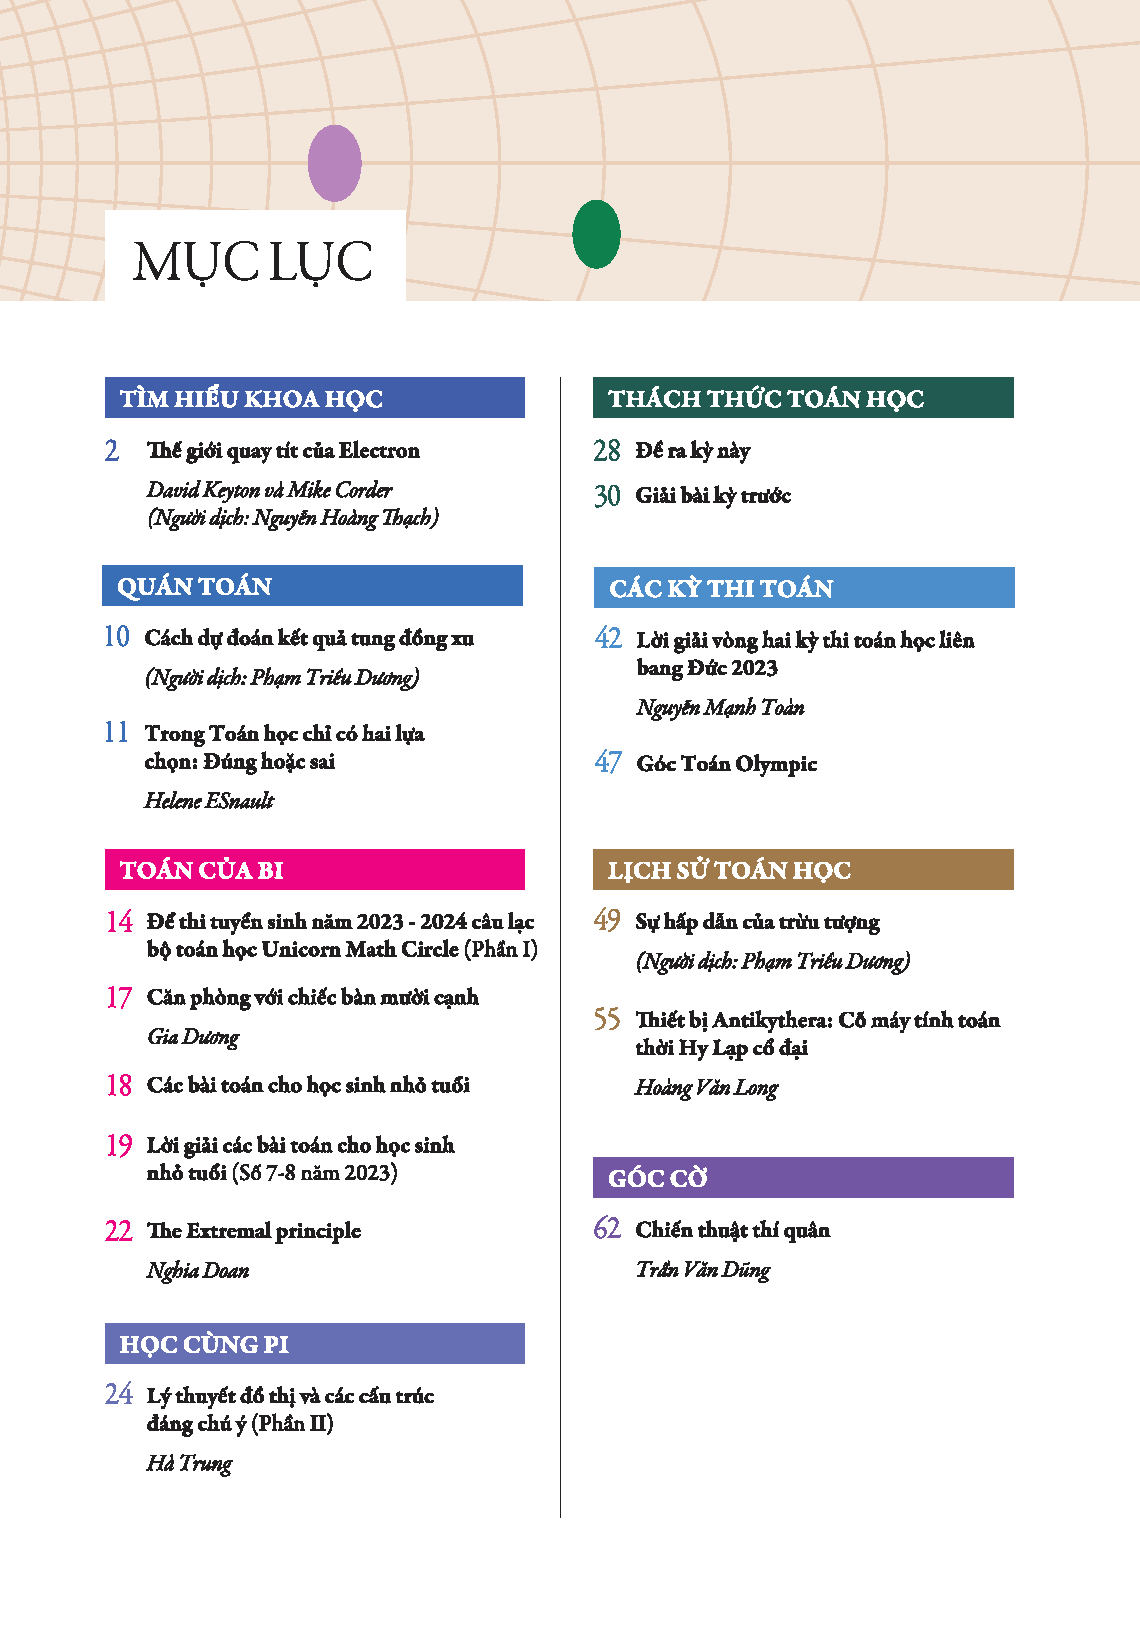
\includegraphics[scale=1]{ML.pdf}}}
%	 \centering
%	 \vspace*{0cm}
%	 \endgroup
%	 \newpage	  
%	 \pagestyle{empty}
%
%	\setcounter{page}{2}
%
	\setcounter{figure}{0}
	\thispagestyle{duongvaotoanhocnone}
\pagestyle{duongvaotoanhoc}
\everymath{\color{duongvaotoanhoc}}
\graphicspath{{../duongvaotoanhoc/pic2/}}
\blfootnote{$^*$\color{duongvaotoanhoc}Nguồn: https://www.quantamagazine.org/hobbyist-finds-maths-elusive-einstein-tile-20230404.}
\blfootnote{\color{duongvaotoanhoc}$^1$THPT chuyên Hà Nội -- Amsterdam.}
\begingroup
\AddToShipoutPicture*{\put(0,616){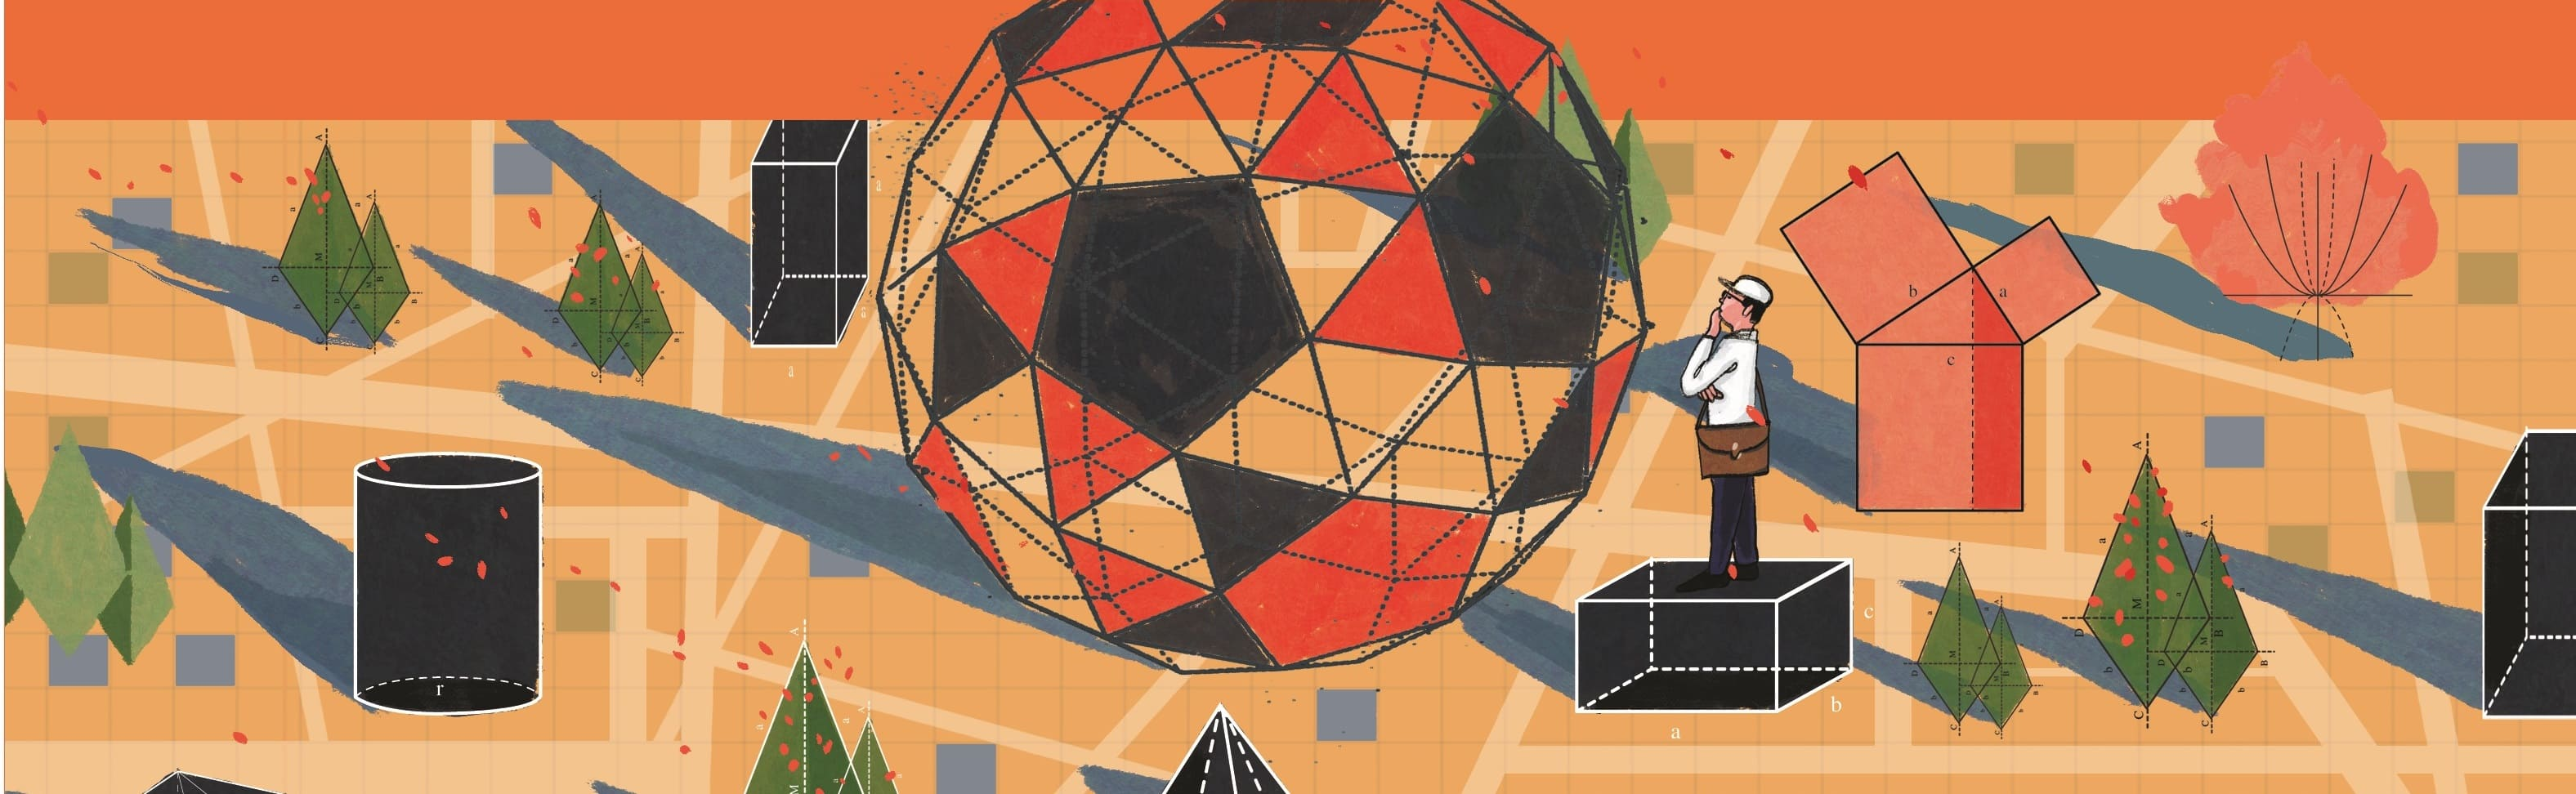
\includegraphics[width=19.3cm]{../bannerduongvao}}}
\AddToShipoutPicture*{\put(76,500){
\includegraphics[scale=1]{../tieude1.pdf}}}
\centering
\endgroup
\vspace*{208pt}

\begin{multicols}{2}	
	Giữa tháng $11$ năm $2022$, David Smith [$1$], một kỹ thuật viên in ấn đã nghỉ hưu có niềm vui thú với xếp hình, hình học fractal và bản đồ đường xá, đang làm việc mình yêu thích: chơi với những hình khối. Nhờ một phần mềm gọi là ``PolyForm Puzzle Solver" [$2$], ông đã dựng được một miếng gạch hình cái mũ trông khá khiêm tốn. Ông đã bắt đầu thử nghiệm xem có thể phủ kín được bao nhiêu phần màn hình với duy nhất viên gạch lát này, với điều kiện không để hai viên đè lên nhau hay để hở khoảng trống.
	\vskip 0.1cm
	Thường thì khi ông tạo ra loại gạch mới, chúng sẽ hoặc tạo thành một họa tiết lặp, hoặc chỉ lát được một phần nhỏ màn hình. Viên gạch mũ có vẻ không thuộc cả hai loại này. Thế là Smith cắt $30$ miếng giấy bìa màu hình viên gạch này và xếp chúng trên bàn. Rồi ông cắt thêm $30$ cái nữa và tiếp tục xếp. ``Tôi dần nhận ra rằng mỗi lần xếp là một cách lát tôi chưa thấy bao giờ," ông nói. ``Đó là một viên gạch lát ranh mãnh". Ông gửi mô tả về viên gạch tới Craig Kaplan [$3$], một nhà khoa học máy tính ông quen tại Đại học Waterloo, Canada. Kaplan ngay lập tức bắt đầu tìm hiểu các tính chất của nó.
	\vskip 0.1cm
	Ngày $20$ tháng $3$ vừa qua, Smith và Kaplan, cùng với $2$ nhà nghiên cứu nữa, đã công bố [$4$] rằng đây chính là thứ mà các nhà toán học đã tìm kiếm suốt hơn năm thập kỉ: một viên gạch duy nhất mà ta có thể dùng để lát toàn mặt phẳng, nhưng chỉ theo những họa tiết không lặp lại bất kỳ khối gạch nào. Các nhà toán học gọi những viên gạch, hoặc các bộ viên gạch, có tính chất đó là ``phi tuần hoàn" (aperiodic), trái với hình vuông hoặc lục giác là những hình có thể phủ cả mặt phẳng theo các họa tiết lặp lại (hay ``tuần hoàn").
	\vskip 0.1cm
	Viên gạch mũ ẩn chứa ``đủ sự phức tạp để bẻ gãy trật tự tuần hoàn theo mọi quy mô", các nhà nghiên cứu khẳng định trong bài báo. Hơn nữa, họ nhận ra rằng viên gạch mũ là một trong vô số viên gạch khác nhau có cùng tính chất này.
	\vskip 0.1cm
	``Tưởng xa tận chân trời mà gần ngay trước mắt,"  là những gì  Doris Schattschneider, giáo sư toán danh dự tại Đại học Moravian, Pennsylvania nói về viên gạch này.  Bà tả rằng bản thân đã ``sửng sốt" trước phát hiện này.
	\vskip 0.1cm
	Các nhà toán học đã bắt đầu tìm kiếm một viên gạch như viên gạch mũ từ những năm 60 thế kỷ trước, khi Robert Berger  [$5$] dựng ra $20426$ loại gạch cùng nhau lát mặt phẳng một cách phi tuần hoàn. Công trình này là phát súng mở màn cho một cuộc đua dựng ra các bộ gạch có thể lát mặt phẳng phi tuần hoàn bằng ít loại hơn, lên đến đỉnh điểm là khám phá của Roger Penrose vào thập niên $70$ với chỉ hai viên. Năm $1982$, Dan Shechtman [$6$] đã tìm ra những dạng đối xứng tương tự như của gạch lát Penrose trong tự nhiên, dưới hình hài các cấu trúc gọi là giả tinh thể (quasicrystal), qua đó giúp ông đạt giải Nobel Hóa học năm $2011$.
	\begin{figure}[H]
		\vspace*{-5pt}
		\centering
		\captionsetup{labelformat= empty, justification=centering}
		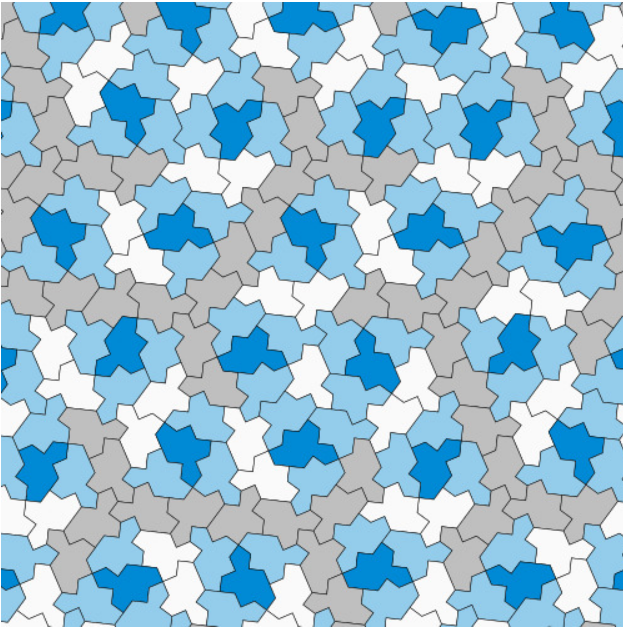
\includegraphics[width= 1\linewidth]{1}
		\caption{\small\textit{\color{duongvaotoanhoc}Viên gạch mũ chỉ là một trong một họ các viên gạch phi tuần hoàn}}
		\vspace*{-10pt}
	\end{figure}
	Từ ấy, các nhà toán học vẫn không ngừng tìm kiếm một loại gạch duy nhất có thể lát mặt phẳng $2$ chiều một cách phi tuần hoàn, mà không cho phép kẽ hở hay gạch đè lên nhau. Ludwig Danzer, một nhà hình học người Đức, đã tinh nghịch đặt tên cho loại gạch như thế là một ``einstein" -- chơi chữ của cụm từ tiếng Đức ``ein stein", nghĩa là ``một miếng".
	\vskip 0.1cm
	Vào những năm $1990$, hai nhóm khác nhau  [$7$] đã tìm ra cách chồng kề nhau một loại gạch $10$ cạnh để phủ mặt phẳng. Trong thập kỷ sau đó, Joan Taylor [$8$], một nhà toán học nghiệp dư ở Tasmania, đã khám phá ra một hình với nhiều miếng không liền  với nhau  [$9$]. Cùng với Joshua Socolar [$10$], một nhà vật lý tại Đại học Duke, họ đã chứng minh được hình này có thể lát mặt phẳng một cách phi tuần hoàn  [$11$]. Và mới năm ngoái, Rachel Greenfield [$12$] từ Viện Nghiên cứu Cao cấp Princeton và Terence Tao [$13$] từ Đại học California, Los Angeles đã phát hiện ra một hình trong không gian nhiều chiều [$14$] có thể lát không gian một cách phi tuần hoàn mà không cần quay hay lật.
	\vskip 0.1cm
	Nhưng chưa ai tìm được một ``einstein" đích thực -- một hình $2$ chiều đơn giản phủ mặt phẳng một cách phi tuần hoàn. Cuối cùng, giới toán học bắt đầu nghi ngờ sự tồn tại của chúng, theo lời Marjorie Senechal [$15$], một nhà nghiên cứu về lát gạch và giáo sư danh dự tại Đại học Smith. Bà cho biết thêm: việc một ``einstein" đơn giản như viên gạch mũ của Smith lù lù trước mắt, chờ đợi được tìm ra là một sự thật ``khó tin". 
	\vskip 0.1cm
	Theo bà phỏng đoán, có lẽ lý do viên gạch mũ tránh được sự tìm kiếm đến tận bây giờ là do nhiều nhà toán học đã tập trung vào các hình đối xứng kiểu ``cấm kỵ" -- những kiểu mà không thể có trong các loại gạch lát tuần hoàn. Chẳng hạn như gạch lát Penrose có ``đối xứng gấp $5$" (đối xứng qua phép quay $72$ độ quanh tâm), như ở các ngũ giác đều hay hình ngôi sao. Các ngũ giác đều không thể phủ mặt phẳng, nên bắt đầu từ các ``đối xứng gấp $5$" là khởi điểm khá tự nhiên. 
	\vskip 0.1cm
	Trái lại, viên gạch mũ chẳng có đối xứng nào cả, và ``đơn giản đến mức tầm thường", các tác giả bình luận. Cách lát này có quan hệ mật thiết với một cách lát tuần hoàn: lưới tổ ong hình lục giác. Ta có thể tạo ra cách lát hình mũ từ cách lát bằng lục giác như sau: trước hết nối các trung điểm các cặp cạnh đối của lục giác. Lục giác sẽ bị chia thành 6 hình ``cánh diều". Mỗi viên gạch mũ được cấu thành từ $8$ hình cánh diều liền nhau, kết hợp từ các lục giác kề nhau. Bất kỳ ai đầu tư chút sức lực, cùng một cái bút dạ và sàn nhà vệ sinh gạch hình lục giác cũng có thể viền được một cách phủ mặt phẳng bằng hình mũ.  
	\begin{figure}[H]
		\vspace*{-5pt}
		\centering
		\captionsetup{labelformat= empty, justification=centering}
		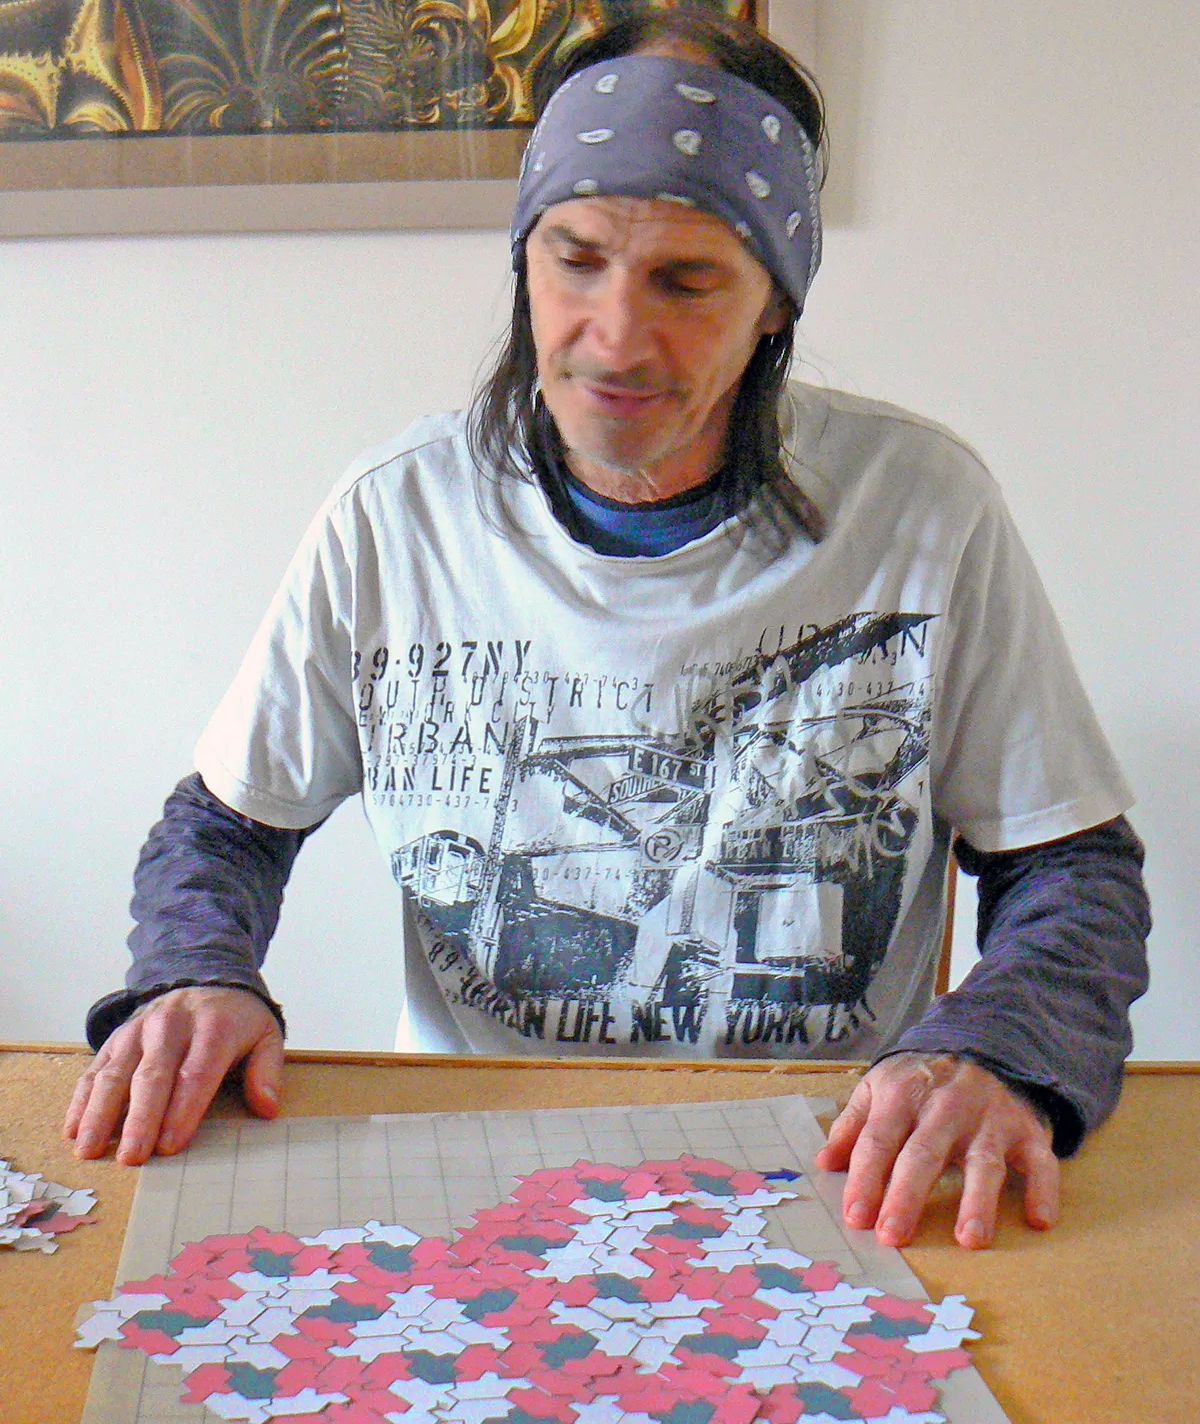
\includegraphics[width= 1\linewidth]{2}
		\caption{\small\textit{\color{duongvaotoanhoc}Khám phá của David Smith được coi là một khám phá khó tin.}}
		\vspace*{-10pt}
	\end{figure}
	Viên gạch mũ, Senechal nói, chỉ ra rằng sự liên kết giữa gạch lát tuần hoàn và phi tuần hoàn chặt chẽ hơn ta tưởng.
	\vskip 0.1cm
	Kể từ lúc thông báo phát hiện này, các nhà toán học và người yêu thích lát gạch đã đổ xô tìm tới những loại gạch mới này, cắt chúng ra từ giấy, in $3$--D, và làm trang trí họa tiết cho mũ và bánh quy của họ. Phong trào ấy đem lại một cảm giác ``hơi siêu thực" cho Smith, một cư dân tại thành phố ven biển Bridlington phía bắc nước Anh. ``Tôi không quen với mấy việc kiểu như thế này".
	\vskip 0.1cm
	Nhưng đây không phải là lần đầu tiên một cá nhân nghiệp dư với niềm đam mê to lớn tạo đột phá trong lát gạch. Robert Ammann, một nhân viên phân loại thư, đã độc lập tìm ra một trong các bộ gạch lát Penrose [$16$] vào những năm $70$. Marjorie Rice, một bà nội trợ ở California, tìm ra cả một họ gạch lát hình ngũ giác [$17$] vào năm $1975$. Và ta có Joan Taylor cùng gạch lát Socolar -- Taylor. Có lẽ những người như họ, khác với các nhà toán học, ``không biết về độ khó của bài toán, vì thế không bị áp lực tâm lý", Senechal nói.
	\vskip 0.1cm
	Với các viên gạch có thể lát mặt phẳng một cách tuần hoàn, thì dùng chúng để lát mặt phẳng một cách không tuần hoàn là tương đối đơn giản. Ví dụ như đặt ngang một vài quân domino trong khi các quân domino khác để dọc. ``Nghệ thuật thực sự là tìm một viên gạch với khả năng lát mặt phẳng, nhưng không thể làm vậy một cách tuần hoàn." Socolar nói.
	\vskip 0.1cm
	Ta không thể tạo ra một thuật toán xác định được liệu một tập hợp các viên gạch nào đó có thể lát mặt phẳng hay không (dù theo cách tuần hoàn hay phi tuần hoàn đi chăng nữa). Nên sau khi được Smith giới thiệu viên gạch mũ, Kaplan đã sử dụng một chương trình ông viết có khả năng đặt các viên gạch bao quanh một viên gốc và mở rộng dần dần từ đó. Ngoài các viên gạch lát mặt phẳng tuần hoàn, chưa ai từng tìm được loại gạch lát nào mà có thể lát quá $6$ vòng quanh viên gạch gốc. Lần này, chương trình cứ chạy và chạy mãi, và nó lát tới tận $16$ vòng gạch mũ trước khi Kaplan dừng chương trình vì đã thu thập đủ dữ liệu.
	\vskip 0.1cm
	Trong khi đó, trước sự kinh ngạc của Kaplan, Smith có một khám phá mới: một viên gạch thứ hai, hình dạng giống một con rùa, cũng thuộc loại phi tuần hoàn. ``Chỉ ra được $2$ einstein liên tiếp thật là ngoài sức tưởng tượng," nhóm nghiên cứu viết.
	\vskip 0.1cm
	Giữa tháng $1$, Smith và Kaplan đã tuyển dụng được $2$ nhà nghiên cứu nữa: Chaim Goodmain--Strauss [$18$], một nhà toán học ở Bảo tàng Toán học Quốc gia và Đại học Arkansas, và Joseph Samuel Myers [$19$], một kỹ sư phần mềm ở Cambridge, Anh, với bằng tiến sỹ tổ hợp. Myers dốc toàn bộ thời gian rảnh của mình cho viên gạch mũ, và chỉ trong hơn một tuần, ông đã chứng minh được nó phi tuần hoàn. ``Chúng tôi khá sốc bởi tốc độ ông ấy giải bài toán này," Kaplan nói.
	\begin{figure}[H]
		\vspace*{5pt}
		\centering
		\captionsetup{labelformat= empty, justification=centering}
		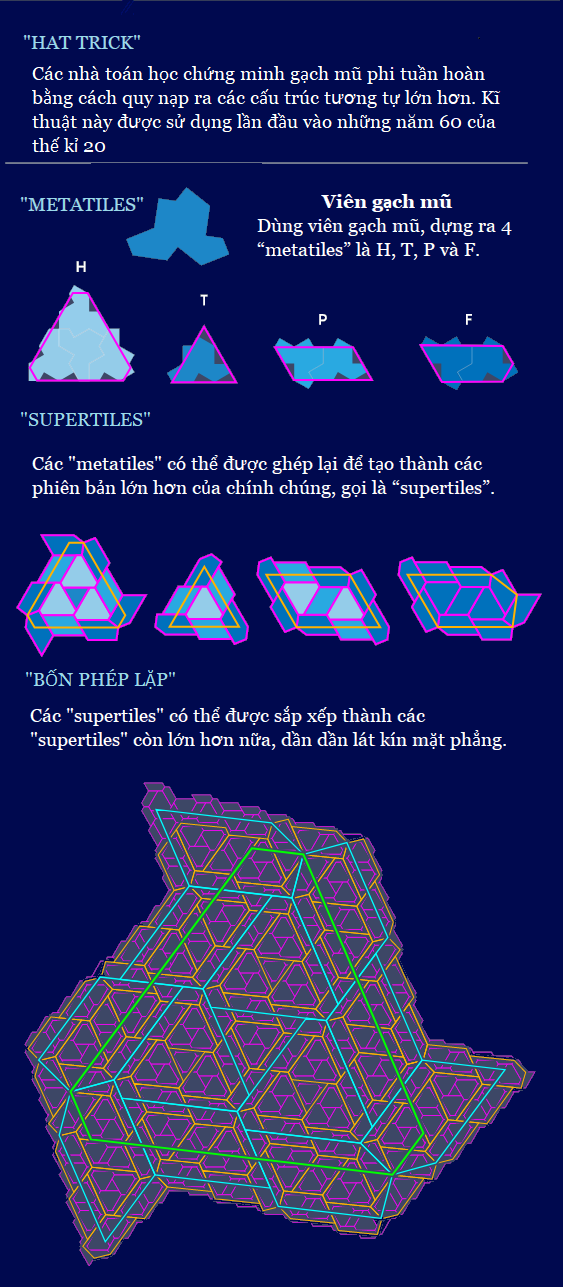
\includegraphics[width= 1\linewidth]{3}
		%		\caption{\small\textit{\color{}}}
		\vspace*{-20pt}
	\end{figure}
	Chứng minh này được biến tấu từ một phương pháp của Berger vào những năm $1960$. Phương pháp đó bao gồm việc ghép một số viên gạch lại với nhau, tạo thành những phiên bản lớn hơn của chính chúng, hình thành một cấu trúc phân chia đẳng cấp. Đầu tiên, Myers xác định bốn hình trung gian được tạo từ viên gạch mũ, gọi là $H$, $T$, $P$ và $F$. Ví dụ, viên gạch $H$ được tạo ra từ $4$ viên gạch mũ, ghép lại thành một hình hao hao một tam giác cụt ở các góc. Myers chứng minh rằng có thể ghép $4$ hình lại với nhau để tạo ra vẫn $4$ hình đó với kích thước lớn hơn. Chẳng hạn, có thể tạo ra một viên gạch $H$ lớn bằng cách xếp ba viên gạch $H$ quanh một viên gạch $T$, rồi ghép các viên gạch $P$ và $F$ xung quanh hình vừa tạo.
	\vskip 0.1cm
	Phương pháp này giúp ta dựng ra những viên gạch lớn dần. Có thể bắt đầu với bất kỳ loại gạch nào, chẳng hạn như viên gạch $H$, phóng to nó lên, và lấp đầy các khe hở  bằng $4$ hình trung gian $H$, $T$, $P$, $F$. Ta có thể lặp đi lặp lại việc này vô số lần để tạo ra một cấu trúc phân cấp từ những hình này, từ đó lát kín mặt phẳng. Đơn vị cơ bản của cấu trúc chính là những viên gạch mũ. 
	\vskip 0.1cm
	Họ đã chứng minh được cách lát hình thành từ các cấu trúc phân cấp này không bao giờ tuần hoàn. Đồng thời họ cũng chỉ ra rằng đó là cách duy nhất để phủ mặt phẳng bằng các hình mũ. Vì thế nên cách phủ mặt phẳng bằng các viên gạch mũ không thể tuần hoàn. ``Một kết quả rất tuyệt vời", Socolar cho hay.
	\vskip 0.1cm
	Vậy là còn lại loại gạch lát thứ hai Smith phát hiện: con rùa. Liệu chăng việc một người đàn ông khám phá ra tận hai loại lát gạch phi tuần hoàn cùng lúc, trong khi phần còn lại của nhân loại bó tay trong suốt 50 năm, đơn thuần là một sự trùng hợp tuyệt diệu? Viên gạch mũ và ``con rùa" nhìn giống nhau đến bất ngờ, khiến các nhà nghiên cứu nghi ngờ rằng con rùa cũng là một viên gạch phi tuần hoàn. Nhưng nghi ngờ vẫn chỉ là nghi ngờ, không phải chứng minh.
	\vskip 0.1cm
	Thế rồi Myers có một khám phá: hóa ra, cả cái mũ và con rùa đều thuộc về một họ gồm vô số viên gạch lát mặt phẳng theo cùng một cách.
	\vskip 0.1cm
	Mỗi viên gạch mũ có $13$ cạnh: $6$ dài, $6$ ngắn tương ứng với các cạnh hình cánh diều, cộng với một cạnh ghép từ hai cạnh cánh diều ngắn. Bằng cách thay đổi kích cỡ độ dài các cạnh của viên gạch mũ, ta có thể thu được vô hạn không đếm được các viên gạch phi tuần hoàn. Tưởng tượng một thanh trượt: di sang trái khiến cạnh ngắn (cùng với một cạnh ghép kể trên) ngắn đi; di sang phải thì cạnh dài nhỏ lại. ``Con rùa" nằm về bên phải so với viên gạch mũ, nhưng đồng thời cũng có vô số hình khác thuộc kiểu tương tự.
	\vskip 0.1cm
	Nếu ta đẩy thanh trượt hết nấc về bên trái, cạnh ngắn sẽ biến mất, viên gạch lúc này có hình chữ $V$ $6$ cạnh;  đẩy hết nấc sang phải thì cạnh dài biến mất và ta được một hình bảy cạnh được đặt tên là ``sao chổi".  Khác với viên gạch mũ, gạch hình chữ $V$ và hình sao chổi có thể được dùng để lát mặt phẳng một cách tuần hoàn. Hình ở trung tâm thanh trượt, tức cạnh dài và cạnh ngắn bằng nhau, cũng có tính chất này.
	\begin{figure}[H]
		\vspace*{-5pt}
		\centering
		\captionsetup{labelformat= empty, justification=centering}
		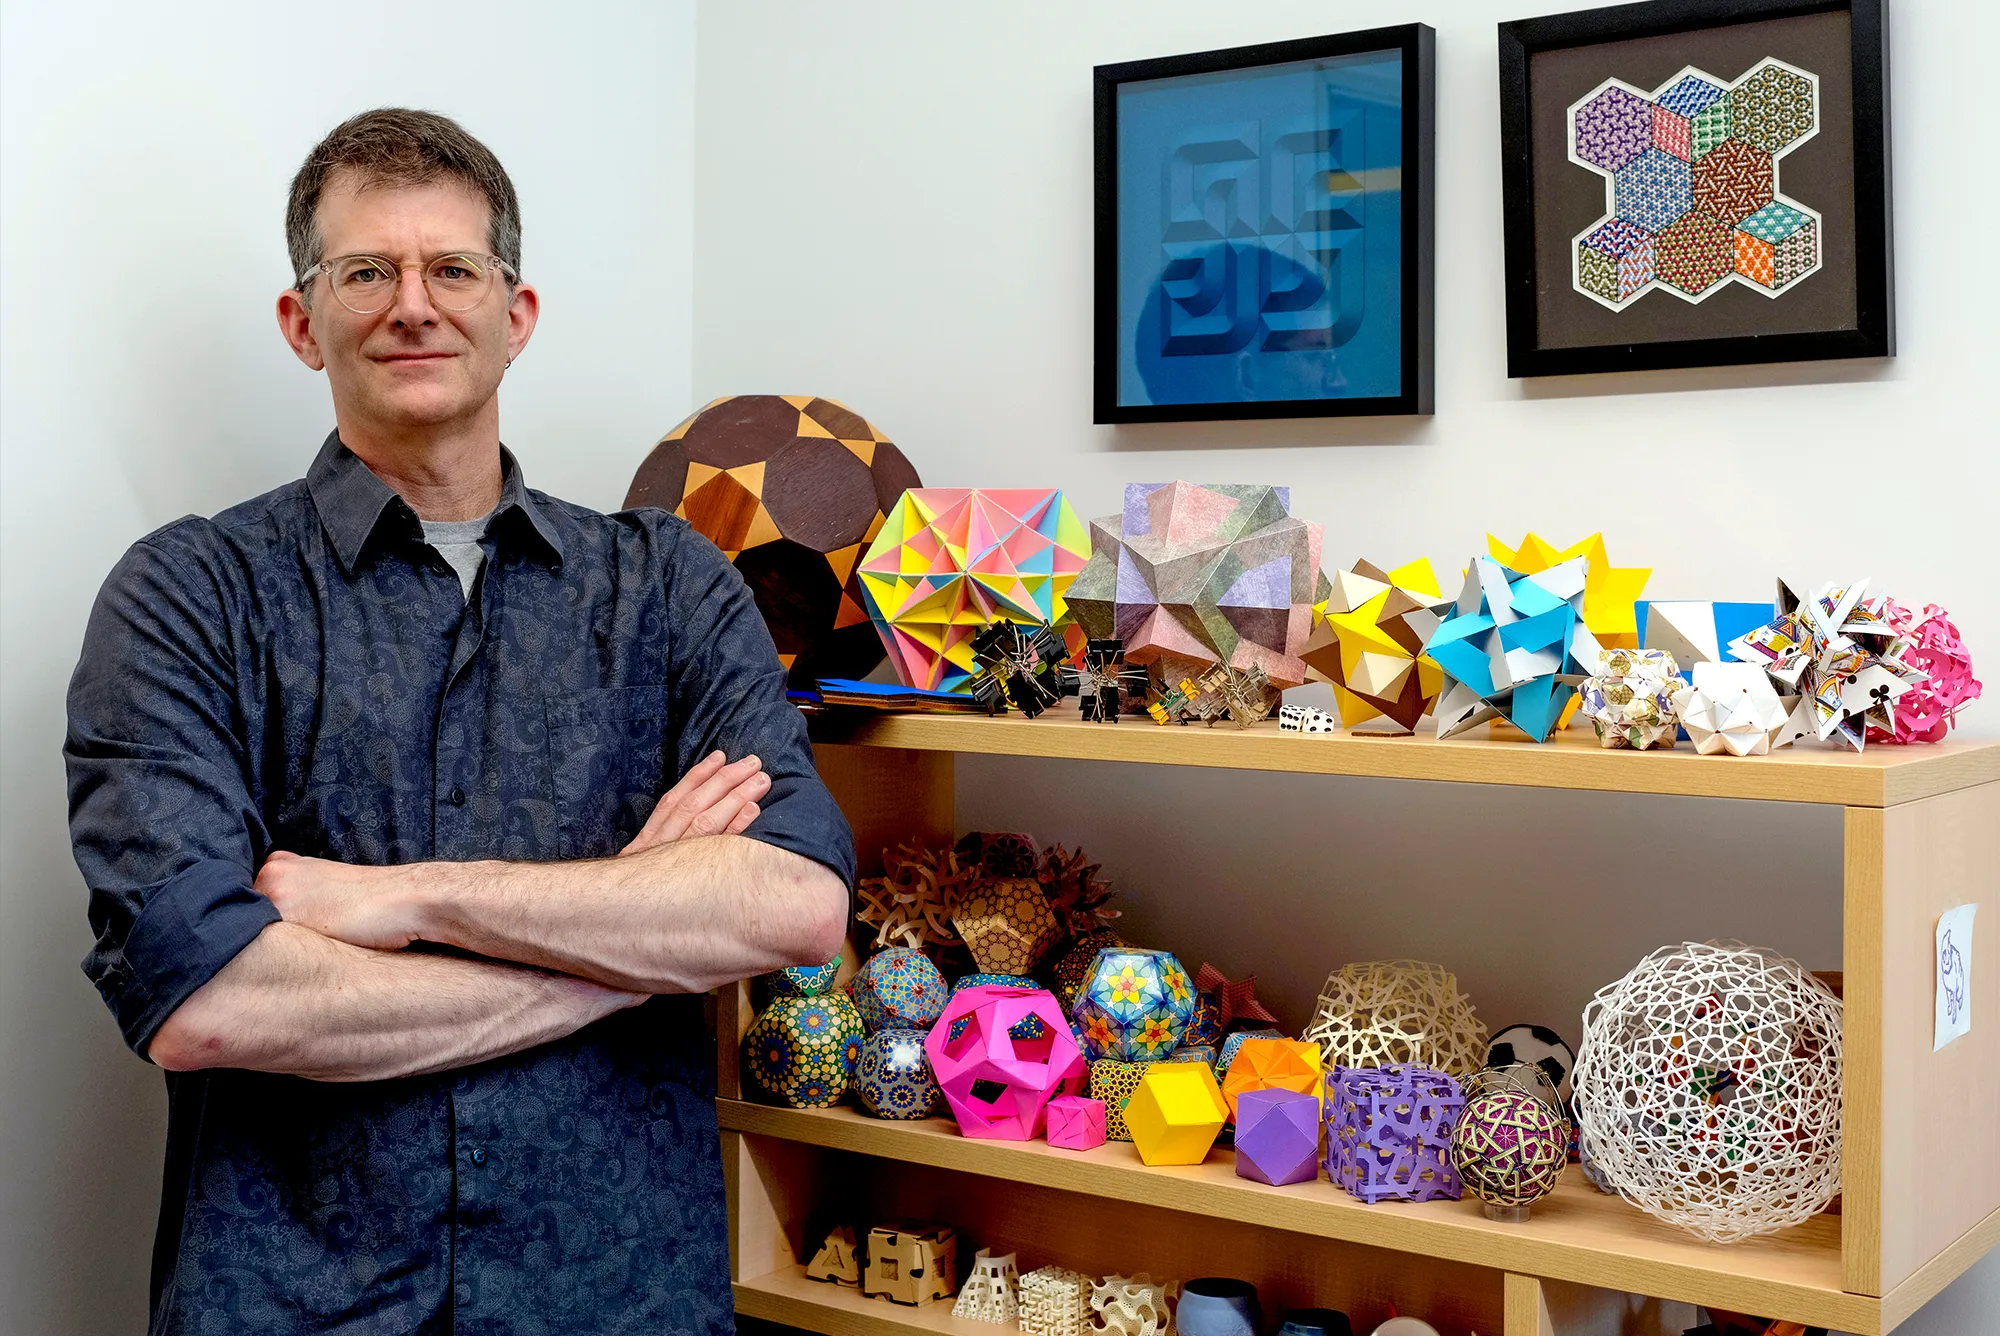
\includegraphics[width= 1\linewidth]{6}
		\caption{\small\textit{\color{duongvaotoanhoc}Craig Kaplan, nhà khoa học máy tính ở đại học Waterloo, Canada.}}
		\vspace*{-10pt}
	\end{figure}
	Myers còn nhận ra rằng mình có thể sử dụng đặc tính hình học của viên gạch chữ $V$ và sao chổi để chứng minh là tất cả các hình dọc theo thanh trượt, trừ hai đầu và trung điểm, đều là gạch loại phi tuần hoàn. Lập luận này, được Kaplan gọi là ``một nước đi thiên tài của Toán học", hoàn toàn mới lạ với bộ môn lát gạch. Trước đây, lĩnh vực này chỉ có $3$ cách tiếp cận chính để chứng minh tính phi tuần hoàn, theo lời Goodman-Strauss. ``Giờ ta có cách thứ tư." 
	\vskip 0.1cm
	Các nhà toán học đang cố gắng thấm phương pháp chứng minh mới này. ``Tôi phải ngồi lại và nghiêm túc dành thời gian cho thứ này," Senechal nói. 
	\vskip 0.1cm
	Một câu hỏi tự nhiên, Greenfield nói, là liệu rằng có thể tìm được một nguồn nào đó tạo ra các cách lát mới không. Năm $1981$, Nicholaas de Brujin [$20$] đã chứng minh được các cách lát Penrose là hình chiếu xuống không gian $2$ chiều của các viên gạch lát tuần hoàn mặt phẳng $5$ chiều. ``Nếu tương tác hoặc cấu trúc của những cách lát (mới) này tương ứng với một cách lát gạch tuần hoàn trên không gian nhiều chiều hơn, điều ấy sẽ thực sự thú vị để tìm hiểu." Greenfield nói.
	\vskip 0.1cm
	Với tư cách một nhà vật lý, Socolar đã bắt đầu khám phá tính chất vật liệu của cách lát mới này. Ông thấy rằng: kiểu nhiễu xạ khi ánh sáng chiếu qua loại gạch lát này có những đỉnh dốc tương tự như ở giả tinh thế. Kể cả khi ấy, cách lát bằng gạch hình mũ vẫn ``trông khác hẳn với tất cả những thứ tôi từng thấy trước đây", ông khẳng định.
	\vskip 0.1cm
	Trong lúc ấy, Smith chưa xong việc với viên gạch ranh mãnh của ông. Ông hiện dự định khám phá tiềm năng nghệ thuật và cách phối màu để làm nổi bật họa tiết của các viên gạch này. ``Dường như nó có thái độ riêng," ông nói. ``Tôi nghĩ ta nên tôn trọng khi làm việc với nó."
	\vskip 0.1cm
	Bình luận của các dịch giả: Có ý kiến cho rằng cái mũ chưa thể được tính là ``einstein" do thực chất chúng ta cần dùng tới cả cái mũ và viên gạch đối xứng trục với nó để lát toàn mặt phẳng, và hai viên gạch có thể tính là khác nhau. Tuy nhiên, đúng như lời hứa, David Smith đã có một phát hiện mới: một trong các họ hàng đặc biệt của cái mũ, gọi là Tile($1, 1$), có thể lát mặt phẳng một cách phi tuần hoàn nếu như ta cấm úp ngược viên gạch lại để ghép. Bằng cách điều chỉnh các cạnh của Tile($1, 1$), ông thu được một họ các viên gạch gọi là bóng ma. Lần này, mỗi bóng ma đều tự nó lát được mặt phẳng phi tuần hoàn, kể cả khi cho phép úp ngược viên gạch này để ghép. Bài báo về phát hiện này [$21$] được đăng lên arXiv vào cuối tháng $5$ năm $2023$, tại thời điểm đăng bài hiện chúng tôi chưa rõ tính xác thực.
	\vskip 0.1cm
	\textbf{\color{duongvaotoanhoc}Các liên kết trong bài viết}
	\vskip 0.1cm 
	[$1$] https://the-orangery.weebly.com/
	\vskip 0.1cm
	[$2$] https://www.jaapsch.net/puzzles/polysol\\
	ver.htm
	\vskip 0.1cm
	[$3$] https://cs.uwaterloo.ca/~csk/
	\vskip 0.1cm
	[$4$] https://arxiv.org/abs/2303.10798
	\vskip 0.1cm
	[$5$] https://www.ams.org/books/memo/00\\
	66/
	\vskip 0.1cm
	[$6$] https://www.engineering.iastate.edu/peo\\
	ple/profile/dannys/
	\vskip 0.1cm
	[$7$] https://link.springer.com/article/10.1007/\\
	BF00239998
	\vskip 0.1cm
	[$8$] http://taylortiling.com/
	\vskip 0.1cm
	[$9$] https://sfb701.math.uni-bielefeld.de/prep\\
	rints/sfb10015.pdf
	\vskip 0.1cm
	[$10$] https://scholars.duke.edu/person/socolar
	\vskip 0.1cm
	[$11$] https://arxiv.org/abs/1003.4279v2
	\vskip 0.1cm
	[$12$] https://www.math.ias.edu/~rgreenfeld/
	\vskip 0.1cm
	[$13$] https://www.math.ucla.edu/~tao/
	\vskip 0.1cm
	[$14$]https://www.quantamagazine.org/nasty-geometry-breaks-decades-old-tiling-conjectur\\
	e-20221215/
	\vskip 0.1cm
	[$15$] http://www.science.smith.edu/~senechal/
	\vskip 0.1cm
	[$16$] https://link.springer.com/article/10.1007\\
	/BF02985414
	\vskip 0.1cm
	[$17$] https://www.quantamagazine.org/marjo\\
	rie-rices-secret-pentagons-20170711/
	\vskip 0.1cm
	[$18$]https://fulbright.uark.edu/departments/\\
	math/directory/index/uid/strauss/name/Chai\\m+Goodman-strauss/
	\vskip 0.1cm
	[$19$] https://www.polyomino.org.uk/
	\vskip 0.1cm
	[$20$] https://www.sciencedirect.com/science/\\
	article/pii/1385725881900172?via\%3Dihub
	\vskip 0.1cm
	[$21$]
	https://arxiv.org/abs/2305.17743
\end{multicols}
	\newpage

	\setcounter{figure}{0}
	\thispagestyle{duongvaotoanhocnone}
\pagestyle{duongvaotoanhoc}
\everymath{\color{duongvaotoanhoc}}
\graphicspath{{../duongvaotoanhoc/pic/}}
\blfootnote{$^*$\color{duongvaotoanhoc}Xuất bản lần đầu trong: The Mathematical Intelligencer $10$, Springer, Berlin Heidelberg New York ($1975$) và được trích lại trong [$1$]}
\begingroup
\AddToShipoutPicture*{\put(0,616){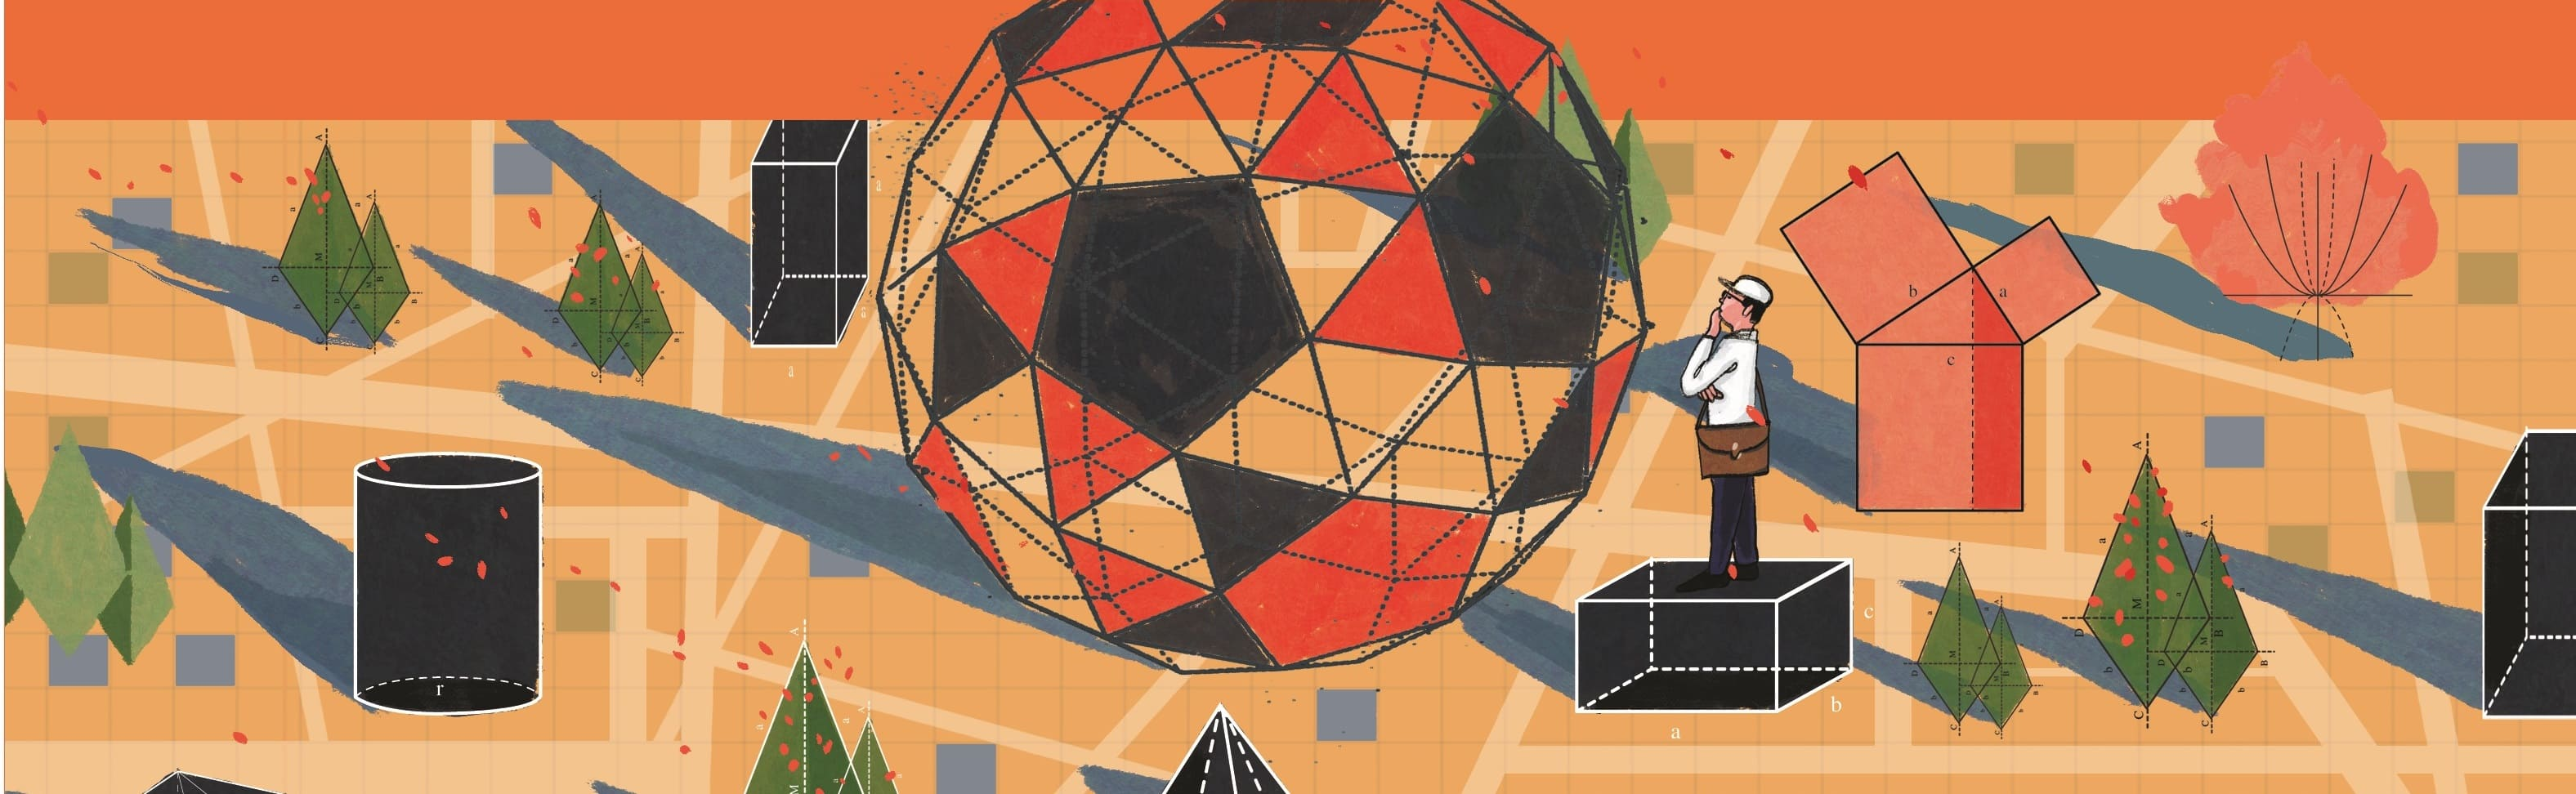
\includegraphics[width=19.3cm]{../bannerduongvao}}}
\AddToShipoutPicture*{\put(80,528){
\includegraphics[scale=1]{../tieude.pdf}}}
\centering
\endgroup

\vspace*{180pt}

\begin{multicols}{2}	
	Câu chuyện của ``các giả thuyết Weil" là một ví dụ kỳ diệu của trí tưởng tượng toán học, và là một trong những thí dụ đáng ngạc nhiên nhất biểu lộ sự thống nhất cơ bản của toán học. Những ý tưởng cốt lõi dẫn tới chứng minh của chúng tới từ sáu người: E. Artin, F. K. Schmidt, H. Hasse, A. Weil, A. Grothendieck, và P. Deligne, trong khoảng năm mươi năm ($1923-1973$).
	\vskip 0.1cm
	$\pmb{1.}$ \textbf{\color{duongvaotoanhoc}Số nghiệm của phương trình đồng dư}
	\vskip 0.1cm
	Một cách đủ thích hợp, câu chuyện, như mọi vấn đề trong lý thuyết số, bắt đầu từ Gauss. Trong công trình về luật thuận nghịch bình phương của mình, ông đưa ra cái ngày nay được gọi là tổng Gauss (phổ biến nhất là tổng $\sum_{x=0}^{p-1} \mathrm{exp}(2\pi i x^2/p)$ với $p$ nguyên tố); để tính các tổng này, bằng một số lập luận sơ cấp, ông suy ra cần tính số nghiệm của các phương trình đồng dư có các dạng 
	\begin{align*}
			&ax^3 - by^3 \equiv 1 \ (\mathrm{mod} \ p),\\ 
			& ax^4 - by^4 \equiv 1 \ (\mathrm{mod} \ p), \tag{$1$}\\ 
			&y^2 \equiv ax^4 - 1 \ (\mathrm{mod} \ p)  
	\end{align*}
	trong đó $a,b$ là các số nguyên cố định không chia hết cho $p$, nghiệm $(x,y)$ được xét theo đồng dư modulo $p$ (như vậy các phương trình đồng dư $(1)$ được xem như các phương trình trong trường $\mathbb{F}_p$); và $p$ \textit{chạy} trong một tập vô hạn các số nguyên tố; chúng ta đi tìm những biểu diễn \textit{tiệm cận} (dưới dạng những hàm đơn giản của $p$) của số lượng các nghiệm. Một thời gian ngắn sau, Jacobi nhận xét rằng, ngược lại, bằng cách sử dụng các tính chất cơ bản của tổng Gauss, ta có thể thu được một đánh giá tốt về số nghiệm trong các trường hợp tổng quát hơn, ở đó các phương pháp sơ cấp trở nên cồng kềnh. Sau Jacobi, gần như không có nhiều tiến triển trong chủ đề này cho tới khi Hardy và Littlewood, trong khi nghiên cứu bài toán Waring để đưa ra các tính chất của ``chuỗi kỳ dị", thấy rằng cần phải đưa ra một đánh giá tiệm cận cho số nghiệm của phương trình đồng dư
	\begin{align*}
		x_1^k + ... + x_r^k \equiv 0 \ (\mathrm{mod} \ p), \tag{$2$}
	\end{align*}
	trong đó $p$ là một số nguyên tố chạy tới $+\infty$. Hai ông đã sử dụng phương pháp của Jacobi cho mục đích này; tổng quát hơn, năm $1949$, cả Hua-Vandier và A. Weil đã độc lập chứng minh rằng phương pháp này có thể đánh giá số nghiệm $N$ của những phương trình
	\begin{align*} 
		a_0x_0^{k_0} \!+\! ... \!+\! a_r x_r^{k_r} \!=\! 0 \ (a_0,...,a_r \neq 0)\tag{$3$}
	\end{align*}
	trong mọi \textit{trường hữu hạn} $\mathbb{F}_{q}$ với $q = p^m$ phần tử; kết quả được đưa ra
	\begin{align*}
		N = q^r + O(q^{(r+1)/2}). \tag{$4$}
	\end{align*}
	Kết quả tương tự được đưa ra bởi Davenport $(1931)$ và Mordell $(1933)$ cho các phương trình dạng $y^m = P_n(x)$ trên $\mathbb{F}_p$, trong đó $P_n$ là một đa thức bậc $n$; với một số giá trị $m,n$ nhỏ, họ thu được các đánh giá có dạng $N  = p + O(p^{\phi(m,n)})$ trong đó $1/2 < \phi(m,n) < 1$.
	\vskip 0.1cm
	$\pmb{2.}$ \textbf{\color{duongvaotoanhoc}Về hàm Zêta}
	\vskip 0.1cm
	Hãy để chúng tôi nhắc lại các tính chất cổ điển của hàm zêta Riemann: nó xác định với $\mathscr{R}(s) > 1$ bởi chuỗi $\zeta(s) = \sum_{n=1}^{\infty} n^{-s}$, và thỏa mãn phương trình Euler
	\begin{align*}
		\zeta(s) = \prod_p (1 - p^{-s})^{-1} \tag{$5$}
	\end{align*}
	trong đó tích chạy trên tập tất cả các số nguyên tố. Riemann chứng minh rằng $\zeta$ có thể thác triển thành một hàm phân hình trên mặt phẳng phức với một cực duy nhất tại $s=1$, và nếu đặt
	\begin{align*} 
		\xi = \frac{1}{2}s(s-1)\pi^{-s/2}\Gamma(s/2)\zeta(s),
	\end{align*}
	thì $\xi$ là một hàm chỉnh hình trên toàn bộ mặt phẳng phức và thỏa mãn phương trình hàm $\xi(s) = \xi(1-s)$. Hơn nữa ông đề xuất \textit{giả thuyết Riemann} (vẫn chưa được chứng minh) rằng mọi nghiệm của $\xi$ nằm trên đường thẳng $\mathscr{R}(s)=1/2$. 
	\vskip 0.1cm
	Một thời gian ngắn sau, Dedekind mở rộng lý thuyết của Riemann lên một trường số $K$ (mở rộng hữu hạn của $\mathbb{Q}$), bằng cách định nghĩa $\zeta_K(s) = \sum_{\mathfrak{a}}(N\mathfrak{a})^{-s}$, trong đó $\mathfrak{a}$ chạy trên tất cả các ideal của vành $\mathfrak{o}$ các số đại số nguyên trong $K$, \textit{chuẩn} $N\mathfrak{a}$ là số phần tử của vành $\mathfrak{o}/\mathfrak{a}$. Ông mở rộng công thức Euler thành
	\begin{align*}
		\zeta_K(s) = \prod_{\mathfrak{p}} (1-  (N\mathfrak{p})^{-s})^{-1}, \tag{$6$}
	\end{align*}
	trong đó tích chạy trên tất cả các ideal nguyên tố $\mathfrak{p}$ của $\mathfrak{o}$; rất nhiều năm sau Hecke chứng minh rằng $\zeta_K$ có thể thác triển thành một hàm phân hình và thỏa mãn một phương trình hàm tương tự như phương trình hàm Riemann cho $\xi$. 
	\vskip 0.1cm
	Một cách hình thức, ta thấy rằng phương trình ($6$) chỉ dùng hai tính chất của vành $\mathfrak{o}$: $1)$ $\mathfrak{o}$ là một vành Dedekind: $2)$ trường $\mathfrak{o}/\mathfrak{p}$ là hữu hạn với mọi ideal nguyên tố $\mathfrak{p}$: thật vậy, nếu $\mathfrak{a} = \mathfrak{p}_1^{v_1}...\mathfrak{p}_r^{v_r}$ là một phân tích thành các ideal nguyên tố của ideal $\mathfrak{a}$ thì $\mathfrak{o}/\mathfrak{a}$ đẳng cấu với tích trực tiếp của các $\mathfrak{o}/\mathfrak{p}_i^{v_i}$, và với mọi ideal nguyên tố $\mathfrak{p}$, mỗi $(\mathfrak{o}/\mathfrak{p})$--module $\mathfrak{p}^h/\mathfrak{p}^{h+1}$ đẳng cấu với $\mathfrak{o}/\mathfrak{p}$; điều đó chứng tỏ rằng chuẩn là nhân tính, từ đó suy ra ($6$) một cách hình thức (chứng minh tính hội tụ của tích vô hạn cần một số ước lượng đơn giản về số các ideal nguyên tố với chuẩn cho trước). Năm $1923$, E. Artin nhận xét rằng các tính chất này đúng cho các vành định nghĩa theo cách sau: bắt đầu với một trường hữu hạn $\mathbb{F}_q$, xét trường $K_0 = \mathbb{F}_q(T)$ các phân thức hữu tỷ, và một mở rộng toàn phương $K = K_0(v)$ với $v^2=P(T)$, trong đó $P$ là một đa thức không có nghiệm bội. Khi đó bao đóng nguyên $\mathfrak{o}$ của $\mathbb{F}_q[T]$ trong $K$ thỏa mãn các tính chất $1)$ và $2)$, $\mathfrak{o}/\mathfrak{p}$ là một \textit{mở rộng hữu hạn} của $\mathbb{F}_q$ với mỗi ideal nguyên tố $\mathfrak{p}$; rất dễ để chứng minh chuỗi và tích vô hạn trong định nghĩa của $\zeta_K$ hội tụ với $\mathscr{R}(s)>1$. Hơn nữa Artin còn thấy rằng lý thuyết này đơn giản hơn của Dedekind rất nhiều, lý do là các hàm của ông có thể viết dưới dạng $Z(q^{-s})$ trong đó $Z(u)$ là một \textit{hàm hữu tỷ} với hệ số trong $\mathbb{Q}$; phương trình hàm biểu diễn thương $Z(1/qu)/Z(u)$ bởi một hàm hữu tỷ với không điểm và cực cho trước; ông ấy sau đó giả thuyết rằng không điểm của $Z(u)$ tất cả đều nằm trên đường tròn $\left| u \right| = q^{1/2}$ và tự kiểm chứng giả thuyết này với rất nhiều đa thức $P$ bậc nhỏ. 
	\vskip 0.1cm
	Bây giờ các ideal nguyên tố $\mathfrak{p}$ sao cho $\mathfrak{o}/\mathfrak{p} \cong \mathbb{F}_q$ ($N\mathfrak{p}=q$) tương ứng một-một với các đồng cấu $\mathfrak{o} \to \mathbb{F}_q$; mọi đồng cấu như vậy gửi $(T,v)$ tới $(a,b) \in \mathbb{F}_q^2$ thỏa mãn $b^2=P(a)$. Nói cách khác số nghiệm của phương trình $y^2 = P(x)$ trong $\mathbb{F}_q^2$ chính là số lượng $N_1$ các ideal nguyên tố kiểu này; tuy nhiên từ phương trình Euler ($6$) suy ra luôn rằng 
	\begin{align*} 
		\log Z(u) = N_1 u + \cdots 
	\end{align*}
	gần $u=0$, như vậy nghiên cứu $Z(u)$ giúp ta hiểu về $N_1$. ``Giả thuyết Riemann" của Artin sinh ra đánh giá
	\begin{align*}  
		\left|N_1 -q \right| \leq  c \cdot q^{1/2}, \tag{$7$}
	\end{align*}
	và như vậy làm chặt hơn những kết quả trước đó của ông về bài toán đồng dư của Gauss. 
	\vskip 0.1cm
	$\pmb{3.}$ \textbf{\color{duongvaotoanhoc}Bước vào hình học đại số}
	\vskip 0.1cm
	Cho $k$ là một trường giao hoán bất kỳ, người ta cố gắng hình dung tập nghiệm $(x_1,...,x_r) \in k^r$ của một phương trình $P(x_1,...,x_r)=0$, với $P$ là một đa thức bất khả quy trong $k[T_1,...,T_r]$ xem như một ``siêu mặt đại số affine" (``đường cong" với $r=2$, ``mặt" với $r=3$) trong ``không gian affine" $k^r$, Hơn nữa, với mọi mở rộng trường $K \supset k$, ta có thể xét các nghiệm của $P(y_1,...,y_r)$ với giá trị $y_i$ trong trường $K$ \textit{lớn hơn}, như vậy ta có một ``siêu mặt đại số" $V$ trong ``không gian affine" $K^r$; việc các hệ số của $P$ nằm trong $k$ giờ được thay bởi việc nói $V$ \textit{xác định} trên $k$. Kinh nghiệm cho thấy việc chuyển đổi giữa ngôn ngữ hình học và trực giác sang những đa tạp ``trừu tượng"chỉ có ích khi $K$ là \textit{đóng đại số} (hãy thử nghĩ về $x_1^2+x_2^2+1=0$ khi $k=\mathbb{R}$). Ta sẽ hạn chế sự quan tâm xuống trường hợp $K=\overline{k}$, bao đóng đại số của $k$; hơn nữa, ta chỉ xét các siêu mặt $V$ không kỳ dị trong $\overline{k}^r$, i.e. tại các điểm mà ``siêu phẳng tiếp xúc" được định nghĩa duy nhất theo nghĩa thông thường (có nghĩa là tất cả các đạo hàm riêng không đồng thời triệt tiêu trong $V$). Với mọi điểm $x=(x_1,...,x_r) \in V$, toạ độ $x_i$ nằm trong $\overline{k}$, do đó có một mở rộng hữu hạn nhỏ nhất $k(x)$ của $k$ chứa tất cả $x_j$ và $[k(x):k]=\mathrm{deg}(x)$ được gọi là \textit{bậc} của điểm $x$. Nếu $\mathfrak{m}$ là hạt nhân của đồng cấu $k[T_1,...,T_r] \to \overline{k}$ gửi mỗi $T_i$ tới $x_i$ thì $\mathfrak{m}$ là một ideal cực đại của $k[T_1,....,T_r]$ và $k[T_1,...,T_r]/\mathfrak{m}$ đẳng cấu với $k(x)$; ta viết $k(\mathfrak{m})=k(x)$ và $\mathrm{deg}(\mathfrak{m}) =\mathrm{deg}(x)$; có thể chứng minh rằng mọi ideal cực đại $\mathfrak{m}$ của $k[T_1,...,T_r]$ chứa $P(T_1,...,T_r)$ ứng với một điểm $x$ của $V$ với bậc $\mathrm{deg}(\mathfrak{m})$. 
	\vskip 0.1cm
	Khi $k=\mathbb{F}_q$, đặt
	\begin{align*}
		Z_V(u) = \prod_{P \in \mathfrak{m}}(1 - u^{\mathrm{deg}(\mathfrak{m})})^{-1}; \tag{$8$}
	\end{align*}
	hàm $Z(u)$ định nghĩa bởi E. Artin bằng với hàm $Z_C(u)$, trong đó $C$ là ``đường cong affine" $x_2^2 - P(x_1) = 0$ xác định trên $\mathbb{F}_q$. Một cách tổng quát ta gọi $Z_V$ là \textit{hàm zêta} của $V$. Các điểm của $V$ trong $(\mathbb{F}_q)^r$ là các điểm mà $\mathrm{deg}(x)$ là ước của $n$; hiển nhiên số lượng các điểm như vậy $\leq q^{nr}$, như vậy số lượng các ideal cực đại $\mathfrak{m}$ mà $P \in \mathfrak{m}$, tương ứng với các điểm này, có ước lượng \textit{tiên nghiệm} $\leq q^{nr}$, điều này chứng tỏ rằng ($8$) hội tụ với $u$ nhỏ; hơn nữa, với $u$ nhỏ ta có thể viết
	\begin{align*}
			uZ'_V(u)/Z_V(u) & = \sum_{P \in \mathfrak{m}} \frac{\mathrm{deg}(\mathfrak{m}) u^{\mathrm{deg}(\mathfrak{m})}}{1 - u^{\mathrm{deg}(\mathfrak{m})}} \\ 
			& = \sum_{v=1}^{\infty} \sum_{P \in \mathfrak{m}} \mathrm{deg}(\mathfrak{m}) u^{v\mathrm{deg}(\mathfrak{m})} \\
			&= \sum_{v=1}^{\infty} N_v u^v\tag{$9$}
	\end{align*}
	trong đó $N_v$ là số điểm của $V$ trong $(\mathbb{F}_{q^v})^r$.  
	\vskip 0.1cm
	Cách định nghĩa này có thể mở rộng cho các dạng đa tạp không kỳ dị khác, không nhất thiết phải bị nhúng trong ``không gian affine" $\overline{k}^r$. Nói một cách theo lịch sử, ngôn ngữ của hình học đại số trong lý thuyết của các hàm zêta được giới thiệu vào năm $1931$ bởi F. K. Schmidt, người nghiên cứu các \textit{đường cong xạ ảnh} không kỳ dị trên trường hữu hạn $\mathbb{F}_q$. Ông chứng minh rằng lý thuyết Dedekind--Weber của đường cong đại số trên $\mathbb{C}$ (bao gồm định nghĩa về giống và định lý Riemann--Roch) có thể mở rộng cho đường cong xạ ảnh trên một trường đóng đại số $\overline{k}$ bất kỳ; điều này cho phép ông chứng minh rằng với mọi đường cong xạ ảnh không kỳ dị $C$ với giống $g$ định nghĩa trên $\mathbb{F}_q$, hàm zêta có thể biểu diễn dưới dạng
	\begin{align*} 
		Z_C(u) = P_{2g}(u)/(1-u)(1-qu) \tag{$10$}
	\end{align*}
	trong đó tử số là một đa thức bậc $2g$ với hệ số nguyên và ta có một phương trình hàm
	\begin{align*} 
		Z_C(1/qu) = (qu^2)^{1-g}Z_C(u). \tag{$11$}
	\end{align*}
	``Giả thuyết Riemann" cho $C$ do đó nói rằng các không điểm của $P_{2g}$ nằm trên đường tròn $\left|u \right|=q^{1/2}$; dễ thấy điều này tương đương với bất đẳng thức
	\begin{align*} 
		\left|N_v \!-\! q^v\!-\! 1\right| \!\leq\! 2g \!\cdot\! q^{1/2} \ \text{với mọi} \ v \geq 1. \tag{$12$}
	\end{align*}
	$\pmb{4.}$ \textbf{\color{duongvaotoanhoc}Mơ mộng về Tôpô đại số}
	\vskip 0.1cm
	Quay lại trường hợp siêu mặt $V$ trong $(\overline{\mathbb{F}}_q)^r$, nhận xét rằng các phần tử của $\overline{\mathbb{F}}_q$ thuộc $\mathbb{F}_{q^n}$ chính là những phần tử mà $t^{q^n}=t$. Xét ánh xạ
	\begin{align*}
		\Phi: (x_1,...,x_r) \mapsto (x_1^{q},...,x_r^q)
	\end{align*}
	từ $(\overline{\mathbb{F}}_q)^r$ vào chính nó. Do hệ số của $P$ nằm trong $\mathbb{F}_q$, do đó thỏa mãn $t^q = t$, ta có
	\begin{align*}
		P(\Phi(x)) = (P(x))^q,
	\end{align*}
	do đó $\Phi$ ánh xạ $V$ lên chính nó; hạn chế của $\Phi$ lên $V$ được gọi là cấu xạ Frobenius của $V$. Năm $1936$, Hasse nhận thấy rằng với một đường cong $C$, số $N_v$ chính là số điểm $x \in C$ thỏa mãn $\Phi^v(x) = x$; i.e. $x$ là một \textit{điểm bất động} của $\Phi^v$. Bây giờ, chúng ta hãy bỏ qua chuỗi các sự kiện mang tính niên đại mà giả vờ rằng ta đang làm việc với các đa tạp đại số không kỳ dị ``cổ điển" $X$ trong một không gian xạ ảnh phức. Từ thời của Picard và  Poincaré người ta đã nhận thấy rằng hầu hết các tính chất của các đa tạp đại số được liên hệ chặt chẽ với các tính chất \textit{đồng điều}. Trong phiên bản hiện thời (chủ yếu từ các công trình của Lefschetz và Hodge), với một đa tạp xạ ảnh không kỳ dị bất khả quy $X$ chiều $d$ trên $\mathbb{C}$ (do đó là một đa tạp khả vi chiều $2d$), các tính chất này xoay quanh \textit{đại số đối đồng điều} $H^{\bullet}(X) = \bigoplus_i H^i(X)$ của $X$ trên trường $K$ với \textit{đặc số} $0$; nó là một đại số phân bậc trên $K$, thỏa mãn các tính chất sau:
	\vskip 0.1cm
	($A$) $1.$ Mỗi $H^i(X)$ là một $K$--không gian vector hữu hạn chiều, bằng $0$ ngoại trừ $0 \leq i \leq 2d$;
	\vskip 0.1cm
	$2.$ Tồn tại một đẳng cấu tự nhiên $H^{2d}(X) \overset{\sim}{\longrightarrow} K$, và với mỗi $i$, phép nhân trên $H^{\bullet}(X)$ cho ta một phép ghép cặp không kỳ dị $H^{i}(X) \times H^{2d-i}(X) \to H^{2d}(X) \overset{\sim}{\longrightarrow} K$ (đối ngẫu Poincaré) cho phép ta đồng nhất $H^{2d-i}(X)$ với 
	\begin{align*} 
		H_i(X) = \mathrm{Hom}_K(H^i(X),K),
	\end{align*} 
	\textit{đồng điều} của $K$ tại chiều $i$.
	\vskip 0.1cm
	$3.$ Với các đa tạp không kỳ dị $X, Y$, tồn tại một đẳng cấu tự nhiên của các đại số phân bậc 
	\begin{align*} 
		&H^{\bullet}(X) \otimes H^{\bullet}(Y) \cong H^{\bullet}(X \times Y) \\
		&\text{(công thức Kunneth)}.
	\end{align*}
	($B$) Mọi cấu xạ $f: X \to X$ định nghĩa tự nhiên, với mỗi $i$, một đồng cấu tuyến tính $f^{(i)}:H^i(X) \to H^i(X)$, sao cho các $f^{(i)}$ với $0 \leq i \leq 2d$ cảm sinh một đồng cấu $f^{\bullet}:H^{\bullet}(X) \to H^{\bullet}(X)$ của các đại số phân bậc. Các \textit{điểm bất động} của $f$ là phép chiếu lên $X$ của giao của đồ thị $\Gamma$ của $f$ và đường chéo $\Delta$ của $X \times X$; nếu $\Gamma$ giao \textit{hoành} với $\Delta$ tại mỗi điểm (nghĩa là các không gian tiếp xúc của chúng có giao chỉ là một điểm), số lượng điểm bất động của $f$ được tính bởi \textit{công thức vết Lefschetz}
		\begin{align*} \label{eq:13}
			N  = \sum_{i=0}^{2d} (-1)^i \mathrm{Tr}(f^{(i)}). \tag{$13$}
		\end{align*}
	($C$) Nếu $Y$ là một đa tạp con không kỳ dị của $X$ với chiều $d-1$, các ánh xạ tuyến tính tự nhiên $H^i(X) \to H^i(Y)$ là song ánh với $i \leq d-2$ và đơn ánh với $i = d-1$. 
	\vskip 0.1cm
	($D$) Lấy $h \in H^2(X)$ từ đối ngẫu Poincaré ứng với lớp đồng điều trong $H_{2d-2}(X)$ của một lát cắt siêu phẳng của $X$, và xét $L: a \to ha$ là phép nhân trái bởi $h$ trong $H^{\bullet}(X)$; khi đó $L^{d-i}: H^i(X) \to H^{2d-i}(X)$ là một đẳng cấu với $i \leq d$.
	\vskip 0.1cm
	Một lập luận đại số đơn giản cho thấy nếu một cấu xạ $f: X \to X$ thỏa mãn $f^{(2)}(h) = q \cdot h$ với $q > 0$ là một số hữu tỷ, và nếu $g_i = q^{-i/2}f^{(i)}$ (xem như một tự đồng cấu của $H^{i}(X) \otimes_K \overline{K}$), $g_i$ là song ánh, và $g_i^{-1}$ được đồng nhất với $\text{}^tg_{2d-i}$ bởi đối ngẫu Poincaré. Điều này suy ra rằng nếu $\alpha_{ij}$ là các giá trị riêng của $f^{(i)}$ trong $\overline{K}$, tập các phần tử $q^{i/2}\alpha_{ij}$ trùng với tập các phần tử $\alpha_{2d-i,j}/q^{d-(i/2)}$.
	\vskip 0.1cm
	($E$) Trong mỗi $H^i(X)$ với $i \leq d$ có một không gian con $A^i(X)$ ổn định dưới tác động của $f^{(i)}$ với mọi cấu xạ $f: X \to X$, và trên mỗi $A^i(X)$, ta có thể trang bị một cấu trúc không gian vector trên trường các số hữu tỷ cùng một \textit{tích vô hướng} không kỳ dị, sao cho: với mỗi $f$ thỏa mãn ($D$) thì mỗi $g_i$ là ánh xạ \textit{unita} với tích vô hướng này; điều này suy ra tất cả các giá trị riêng của $f^{(i)}$ (là các phần tử của $\overline{\mathbb{Q}}$) có giá trị tuyệt đối là $q^{1/2}$.
	\vskip 0.1cm
	Quay lại với siêu mặt $V$ xác định trên $\mathbb{F}_q$, \textit{giả sử} ta có thể gán với nó một đại số phân bậc $H^{\bullet}(V)$ có tất cả các tính chất vừa nêu, hơn nữa $\Phi^{(2)}(h) = q \cdot h$ trong đó $\Phi$ là đồng cấu Frobenius. Dễ thấy đồ thị của $\Phi^v$ giao hoành với $\Delta$; do đó, nếu $\alpha_{ij}$ là các giá trị riêng của $(\Phi^v)^{(i)}$, số $N_v$ có thể cho bởi công thức
	\begin{align*} 
		N_v = \sum_i (-1)^i \sum_j \alpha_{ij}^v;\tag{$14$}
	\end{align*}
	và do đó ta có (với $d= r-1=\mathrm{dim}(V)$)
	\begin{align*} \label{eq:15}
		Z_V(u) = \frac{P_1(u)P_3(u)...P_{2d-1}(u)}{P_0(u)P_2(u)...P_{2d}(u)} \tag{$15$}
	\end{align*}
	trong đó $P_i(u) = \mathrm{deg}(1 - u \cdot \Phi^{(i)})$ là một đa thức với hệ số nguyên. Nói riêng, $Z_V(u)$ là một hàm \textit{hữu tỷ}; hơn nữa $Z_V(1/q^d u)$ nên có không điểm và cực giống với $Z_V(u)$ ngoại trừ khi $u=0$, và ta nên có $\left|\alpha_{ij}\right|=q^{1/2}$. Cuối cùng, nếu tất cả hệ số của $V$ là các lớp đồng dư mod $p$ của các số nguyên, hệ số của một phương trình của một đa tạp không kỳ dị $V_0$ trong $\overline{\mathbb{Q}}^r$, bậc của mỗi $P_i$ sẽ bằng số Betti thứ $i$ của $V_0$. 
	\vskip 0.1cm
	Các phát biểu trên là \textit{các giả thuyết Weil} cho $Z_V$.
	\vskip 0.1cm
	$\pmb{5.}$ \textbf{\color{duongvaotoanhoc}Những ``phương án thay thế" cho đối đồng điều của Hasse và Weil} 
	\vskip 0.1cm
	Để hiểu tại sao Weil đã có thể đi tới những khái niệm táo bạo như vậy, ta phải quay lại những ý tưởng đầu tiên của Hasse trong việc chứng minh ``giả thuyết Riemann" cho các đường cong \textit{giống} $1$ trên $\mathbb{F}_q$. Trong lý thuyết cổ điển của các đường cong không kỳ dị trên trường số phức, mỗi đường cong $C$ được gán với \textit{jacobian} $J = J(C)$, có thể xem như đối ngẫu Pontrjagin của nhóm đồng điều $H_1(C,\mathbb{Z})$; đối ngẫu này được dẫn ra từ dạng song tuyến tính $(\gamma,\omega) \mapsto \int_{\gamma}\omega$ định nghĩa trên các chu trình $\gamma$ và các dạng vi phân abel chỉnh hình $\omega$ trên diện Riemann $C$ (``chu kỳ" của $\omega$ trên $\gamma$). Nếu $C$ có giống $g$ thì $J(C)$ là một xuyến phức $\mathbb{C}^g/\Delta$ trong đó $\Delta$ là một nhóm con rời rạc với hạng $2g$, thỏa mãn các điều kiện song tuyến tính Riemann cổ điển. Ta có thể định nghĩa $J$ một cách đại số, bằng cách xét các nhóm cộng $G/G_i$ của các lớp của các ước bậc $0$ trên $C$, modulo quan hệ tương đương tuyến tính: ta gắn mỗi ước $D$ bậc $0$, vốn có thể viết dưới dạng $\partial \gamma$ với $1$-xích $\gamma$ trên diện Riemann, một lớp $\phi(D)$ trong $\mathbb{C}^g/\Delta$ của vector $\left(\int_{\gamma}\omega_1,...\int_{\gamma}\omega_g\right)$, trong đó các $\omega_j$ lập thành một cơ sở của không gian các dạng vi phân chỉnh hình; định lý Abel-Jacobi nói rằng phép tương ứng này là toàn ánh và có hạt nhân $G_i$. Từ đó có thể trang bị cho $J$ một cấu trúc \textit{nhóm đại số} (một trường hợp cụ thể của nhóm đại số trên $\mathbb{C}$ được biết đến như \textit{các đa tạp abel}) với sự giúp đỡ của các điều kiện (siêu việt) song tuyến tính Riemann. Cuối cùng, nếu $x_0$ là một điểm trên $C$,
	\begin{align*}
		x \mapsto \phi((x) - (x_0))
	\end{align*}
	là một cấu xạ từ $C$ vào $J$ và là đẳng cấu nếu $g=1$.
	\vskip 0.1cm
	Phương pháp đầu tiên của Hasse để làm việc với các đường cong $C$ giống $1$ xác định trên $\mathbb{F}_q$ là ``nâng" $C$ thành một đường cong $C_0$ ``cổ điển" giống $1$ xác định trên trường các số hữu tỷ $\mathbb{Q}$: nếu $E$ là trường các hàm hữu tỷ trên $C$, ông chứng minh rằng ta có thể xác định $C_0$ sao cho, nếu $\omega_1,\omega_2$ là các hàm chu kỳ của các hàm elliptic ứng với $C_0$ (nên trường $E_0$ của các hàm này là trường các hàm hữu tỷ trên $C_0$), $\omega_1/\omega_2$ phải sinh ra một trường toàn phương ảo $K$ trên $\mathbb{Q}$, và $E$ sẽ là trường thặng dư của vành các số nguyên của $K$ modulo một ideal nguyên tố khéo chọn nào đó. Hasse từ đó đã có thể dùng các kết quả cổ điển về ``các phép nhân phức" của $C_0$ (i.e. tự đồng cấu của jacobian $J(C_0)$) để xác định số điểm của $C$ với bậc $1$, và chứng minh ``giả thuyết Riemann" cho $C$.
	\vskip 0.1cm
	Một thời gian ngắn sau, Hasse từ bỏ phương pháp trên và thay thế bằng một phương pháp có tính nội tại hơn: như đã nói ở trên, $J(C)$ có thể định nghĩa một cách đại số như một nhóm ``trừu tượng", và cấu xạ Frobenius định nghĩa tự nhiên một tự đồng cấu của nhóm đó; Hasse chứng minh rằng tử số của hàm zêta $Z_C$ trong ($10$) (trong trường hợp này là một đa thức bậc $2$) được đồng nhất với đa thức đặc trưng của tự đồng cấu đó. Công cụ mà ông giới thiệu cho mục đích này là một số nguyên $v(\lambda)$ gắn với mỗi tự toàn cấu $\lambda$ của $J(C)$: nếu $E$ là trường các hàm hữu tỷ của $C$, $\lambda$ định nghĩa một ``đối cấu xạ" (comorphism) $R(\lambda)$, một tự đẳng cấu của $E$ và $v(\lambda)$ là bậc $[E:R(\lambda)(E)]$, hữu hạn khi $\lambda$ là toàn cấu. Hasse chứng minh rằng với mọi số nguyên $a,b$ thì
	\begin{align*} v(a.1 + b.\lambda) = a^2 + \sigma(\lambda)ab + v(\lambda)b^2
	\end{align*} 
	với mọi tự toàn cấu $\lambda$ của $J(C)$, tính xác định dương của dạng toàn phương này cho ông chứng minh của ``giả thuyết Riemann". 
	\vskip 0.1cm
	Việc mở rộng những ý tưởng này cho các đường cong $C$ giống $g$ bất kỳ trên $\mathbb{F}_q$ là không hề hiển nhiên: lý thuyết cổ điển chứng minh rằng $J(C)$ nên là một nhóm đại số $g$ chiều (thay vì đẳng cấu với $C$ như một đa tạp đại số trong trường hợp của Hasse), và cho tới tận năm $1940$ không ai mở rộng lý thuyết của các nhóm đại số trên trường đặc số $p>0$ sang hình học đại số, và nói riêng lý thuyết của các đa tạp abel. Điều này đã được thực hiện một mình bởi A. Weil, người đầu tiên phải phát triển, trong cuốn sách nổi tiếng \textit{Foundations of algebraic geometry}, các tính chất cơ bản của các số giao một cách độc lập mà không viện tới tôpô đại số. Sau đó ông đã có thể nghiên cứu cấu trúc vành của các tự đồng cấu của một đa tạp abel $A$; với mọi tự toàn cấu $\lambda$ của $A$, Weil định nghĩa số nguyên $v(\lambda)$ như Hasse, (bây giờ $E$ là trường các hàm hữu tỷ trên $A$) và lần này chứng minh
	\begin{align*}
		&v(a \cdot 1 + b \cdot \lambda) \\
		= \,&a^{2g} + \sigma(\lambda)a^{2g-1}b +...+ v(\lambda)b^{2g}.
	\end{align*}
	Bất biến $\sigma(\lambda)$ được xem như một ``thay thế" đóng vai trò của $\mathrm{Tr}(f^{(1)})$ khi $\lambda$ là tự đồng cấu của $J(C)$ ứng với một cấu xạ $f$ của $C$. Một ``thay thế" cho đối ngẫu Poincaré được phát hiện trong một đối ngẫu tổng quát cho các đa tạp abel mà có thể định nghĩa nghĩa hoàn toàn đại số (trong trường hợp cổ điển người ta định nghĩa nó bởi đối ngẫu Pontrjagin); cuối cùng, nếu $\lambda'$ là ``chuyển vị" của một tự đồng cấu $\lambda$ trong đối ngẫu này thì ta có thể chứng minh $\sigma(\lambda \lambda') > 0$ với $\lambda \neq 0$, tính chất này (xem như một ``thay thế" cho tính xác định dương của tích vô hướng Hodge) cho phép Weil đưa ra chứng minh của ``giả thuyết Riemann" cho đường cong có giống bất kỳ.
	\vskip 0.1cm
	Trong tất cả các công trình này, Weil đã không ngừng giữ trong trí óc ông lý thuyết cổ điển của các ``tương ứng" phát triển bởi Hurwicz: một tương ứng trên $C$ có thể xem như một cấu xạ ``đa trị", mà cụ thể hơn như một đường cong $\Gamma$ trên diện $C \times C$; tốt hơn nữa, nó được định nghĩa như một ước (tổ hợp tuyến tính của các đường cong) trên $C \times C$. Một tương ứng $\Gamma$ gắn một cách tự nhiên (bắt chước phiên bản lý thuyết tập hợp) mỗi ước $D$ trên $C$ (tổ hợp tuyến tính của các điểm) một ước khác $\Gamma(D)$, một lần nữa điều này định nghĩa một tự đồng cấu của $J(C)$; ngược lại có thể chỉ ra rằng mọi tự đồng cấu của $J(C)$ đều thu được từ cách định nghĩa này. Trong trường hợp cổ điển, công thức Lefschetz ($13$) có thể được mở rộng để cho số giao của một tương ứng $\Gamma$ với ``tương ứng đồng nhất", i.e. đường chéo $\Delta$ của $C \times C$, và thực tế điều này đã được chứng minh bởi Hurwicz vào năm $1866$, sử dụng lý thuyết tích phân abel; sự thật là Weil đã có thể chứng minh một công thức tương tự bằng các công cụ thuần túy đại số, điều đã dẫn ông đến chỗ đề xuất các giả thuyết mang tên mình.
	\vskip 0.1cm
	$\pmb{6.}$ \textbf{\color{duongvaotoanhoc}Đối đồng điều \'etale và định lý của Deligne}
	\vskip 0.1cm
	Sử dụng kết quả của mình cho các đường cong, Weil đã chứng minh được các giả thuyết của chính ông với các siêu mặt dạng ($3$), cũng như cho những đa tạp khác như các đa tạp Grassman. Nhưng tại thời điểm đó không có một lý thuyết đối đồng điều nào đủ ``tốt" đã được định nghĩa. Khoảng năm $1953$, Cartan và Serre đã dùng đối đồng điều Leray với hệ số là các bó như một công cụ cực kỳ hữu hiệu để nghiên cứu các đa tạp phức, và Serre đã chỉ ra làm cách nào để chuyển các kỹ thuật này sang các đa tạp đại số trên một trường đóng đại số với đặc số $p$. Nhưng khi $p>0$, những nhóm đối đồng điều mới đó được định nghĩa hiển nhiên không thể được sử dụng bởi công thức Lefschetz ($13$), trong đó vế trái bắt buộc phải là một số nguyên, mà không phải một phần tử của một trường có đặc số $p$. Chỉ sau khi Grothendieck xây dựng lý thuyết lược đồ mà, từ một lưu ý của Serre, thì cậu ấy đã có thể mở rộng ý tưởng ban đầu theo cả hai hướng ``tôpô" và ``bó", gắn mỗi đa tạp (hoặc lược đồ) $X$ một đại số đối đồng điều $H^{\bullet}(X_{et},\mathbb{Q}_l)$ trên trường $l$--adic $\mathbb{Q}_l$, trong đó $l$ là một số nguyên tố khác với đặc số của trường ban đầu (sự can thiệp của các trường $l$--adic trong những câu hỏi này đã được nhận ra bởi Weil và Deuring).
	\vskip 0.1cm
	Độ sâu sắc và phức tạp của các kỹ thuật liên quan trong định nghĩa của ``đối đồng điều \'etale" $H^{\bullet}(X_{et})$ như thể để loại trừ mọi khả năng trong việc đưa ra bất kỳ một chi tiết nào nữa trong định nghĩa của nó. Hãy để chúng tôi chỉ ra Grothendieck (với sự giúp đỡ của M. Artin (con trai của E. Artin) và J. L. Verdier) đã có thể chứng minh các tính chất ($A$), ($B$), ($C$) \footnote[1]{\color{duongvaotoanhoc}Trước khi đối đồng điều $l$--adic được định nghĩa, Dwork đã chứng minh, bằng cách khéo léo sử dụng các hàm giải tích $p$--adic, rằng hàm zêta $Z_V(u)$ là \textit{hữu tỷ}.} ở trên và gần đây Deligne đã chứng minh ($D$) cũng đúng với mọi đa tạp trên một trường hữu hạn $\mathbb{F}_q$; tuy nhiên không một tính chất nào tương tự như ($E$) đã được chứng minh cho đối đồng điều \'etale (hoặc bất kỳ một lý thuyết đối đồng điều nào được đưa ra gần đây). Các tính chất ($A$), ($B$), ($C$) là đủ để chứng minh ($15$), cũng như phương trình hàm
	\begin{align*}
		Z_V(1/q^d u) = \pm q^{n\chi/2} u^{\chi}Z_V(u)
	\end{align*}
	trong đó
	\begin{align*}
		\chi = \sum_{i=0}^{2d} (-1)^i \mathrm{dim} \ H^i(X_{et},\mathbb{Q}_l).
	\end{align*}
	Tuy nhiên, chỉ đến gần đây người ta mới biết rằng các hệ số của $P_j$ trong ($15$) là độc lập với số nguyên tố $l$. Điều này cuối cùng cũng được chứng minh bởi Deligne năm $1973$, cùng với phần cuối và khó nhất của các giả thuyết Weil là $\left|\alpha_{ij}\right|=q^{1/2}$.
	\vskip 0.1cm
	Ở đây lần nữa, cần nhớ rằng không thể mô tả một cách chi tiết các chứng minh cực kỳ khéo léo, điều này hơi khác với chứng minh của Hasse và Weil, do nó không thể dựa trên một lập luận ``tính dương". Ta hạn chế bài toán xuống trường hợp $i=d$ (i.e. đối đồng điều ``trung tâm" $H^d(X)$); việc chứng minh rằng $\left|\alpha_{dj}\right|=q^{d/2}$ thì tương đương với
	\begin{align*} \label{eq:18}
		q^{(d-1)/2} \leq \left|\alpha_{dj}\right| \leq q^{(d+1)/2} \tag{$18$}
	\end{align*}
	bởi vì nếu ta áp dụng kết quả này với tích $X^k$, và sử dụng công thức Kunneth, ta có
	\begin{align*} 
		q^{(kd-1)/2} \leq \left|\alpha_{dj}^k \right| \leq q^{(kd+1)/2}
	\end{align*}
	sau đó cho $k$ tiến tới $+\infty$ và thu được kết quả. Thậm chí trong ($18$) ta có thể giả sử là $d$ chẵn và sau đó có thể chứng minh bằng quy nạp theo số chẵn $d$; đây là một bước sâu sắc và khó trong chứng minh, dựa trên kỹ thuật ``đơn đạo" cũ từ Picard và Lefschetz: kỹ thuật này hoàn toàn mang tính tôpô trong trường hợp cổ điển, nhưng nó cũng đã được chuyển sang đối đồng điều \'etale bởi Grothendieck và những người cùng trường phái của cậu ấy.
	\vskip 0.1cm
	Như thường thấy trong toán học, sự đột phá này mở ra một con đường trong việc khai phá các vấn đề mới; nhưng chừng nào bài toán ban đầu của Gauss còn được quan tâm, nó là điểm cuối của vấn đề, vì định lý của Deligne suy ra rằng, số các điểm bậc $1$ của một siêu mặt xạ ảnh không kỳ dị $d$ chiều thỏa mãn đánh giá
	\begin{align*} 
		\left| N - (1 + q+...+q^d )\right| \leq bq^{d/2}
	\end{align*}
	trong đó thậm chí hằng số $b$ có thể tính cụ thể: nó là số Betti thứ $d$ của các siêu mặt trên $\mathbb{C}$ có cùng bậc với $V$.
	\vskip 0.1cm
	\textbf{\color{duongvaotoanhoc}Tài liệu tham khảo}
	\vskip 0.1cm
	[$1$] Eberhard Freitag and Reinhardt Kiehl. \textit{Étale cohomology and the Weil conjecture}, volume $13$ of \textit{Ergebnisse der Mathematik und ihrer Grenzgebiete ($3$) [Results in Mathematics and Related
	Areas ($3$)]}. Springer--Verlag, Berlin, $1988$. Translated from the German by Betty S. Waterhouse and William C. Waterhouse, With an historical introduction by J. A. Dieudonné.
\end{multicols}
\vspace*{-10pt}
{\rule{1\linewidth}{0.1pt}}
\vskip 0.25cm
\centerline{\LARGE\textbf{\color{duongvaotoanhoc}LỜI GIẢI, ĐÁP ÁN}}
\begin{multicols}{2}
		\textbf{\color{duongvaotoanhoc}Đố vui}
		\vskip 0.1cm
		Hãy hình dung khối lập phương bao gồm tám khối lập phương đơn vị.
		\begin{figure}[H]
				\vspace*{-10pt}
				\centering
				\captionsetup{labelformat= empty, justification=centering}
				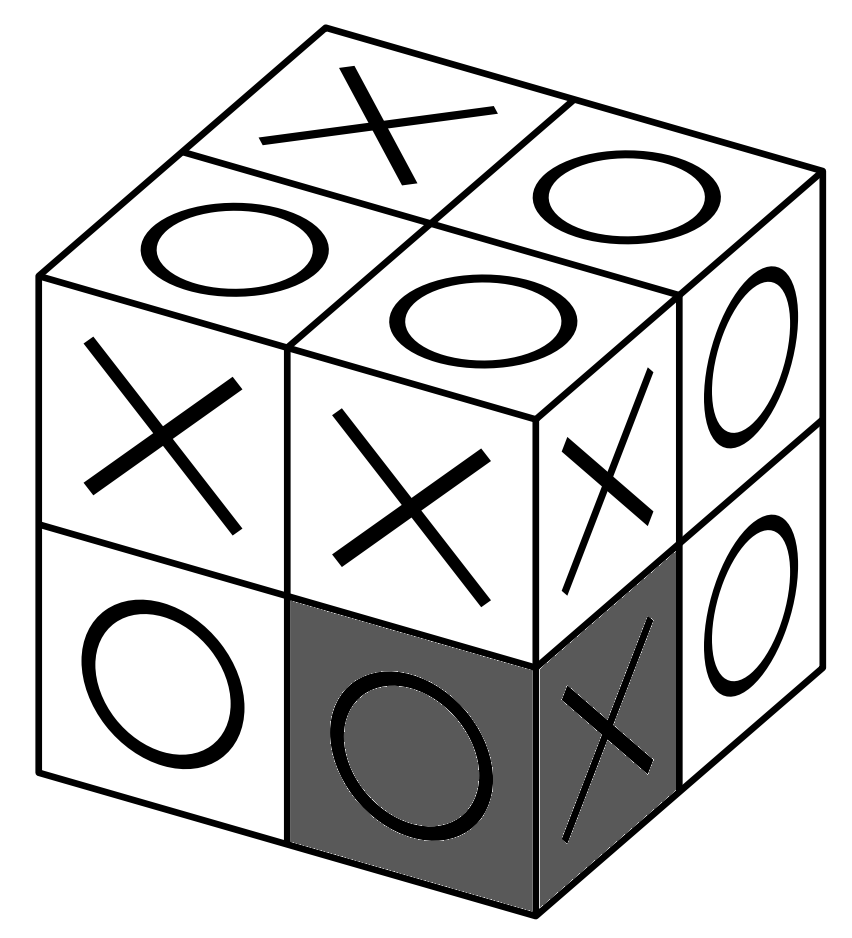
\includegraphics[width= 0.65\linewidth]{lgdovui}
		%		\caption{\small\textit{\color{}}}
				\vspace*{-5pt}
			\end{figure}
		Hãy quan sát khối lập phương đơn vị được tô màu xám như trong hình. Cho dù Bi có điền dấu gì ở mặt bên dưới của khối lập phương này thì cũng không thỏa mãn yêu cầu của thầy giáo: nếu bạn điền dấu $X$ thì mặt chứa dấu $O$ sẽ được bao quanh bởi $3$ ô có dấu $X$ và $1$ ô có dấu $O$, còn nếu bạn điền dấu $O$ thì mặt chứa dấu $X$ sẽ được bao quanh bởi $3$ ô có dấu $O$ và $1$ ô có dấu $X$!
\end{multicols}
	\newpage

%
%	\thispagestyle{empty}
%	\begingroup 
%	\AddToShipoutPicture*{\put(0,0){\includegraphics[width=19.5cm]{MV.pdf}}}
%	\centering
%	\vspace*{0cm}
%	\endgroup
%	\newpage	
%	\pagestyle{empty}
%
	\setcounter{figure}{0}
	\thispagestyle{quantoannone}
\pagestyle{quantoan}
\everymath{\color{quantoan}}
\graphicspath{{../quantoan/pic2/}}
\blfootnote{\color{quantoan}$^1$Viện Vật lý.}
\begingroup
\AddToShipoutPicture*{\put(0,616){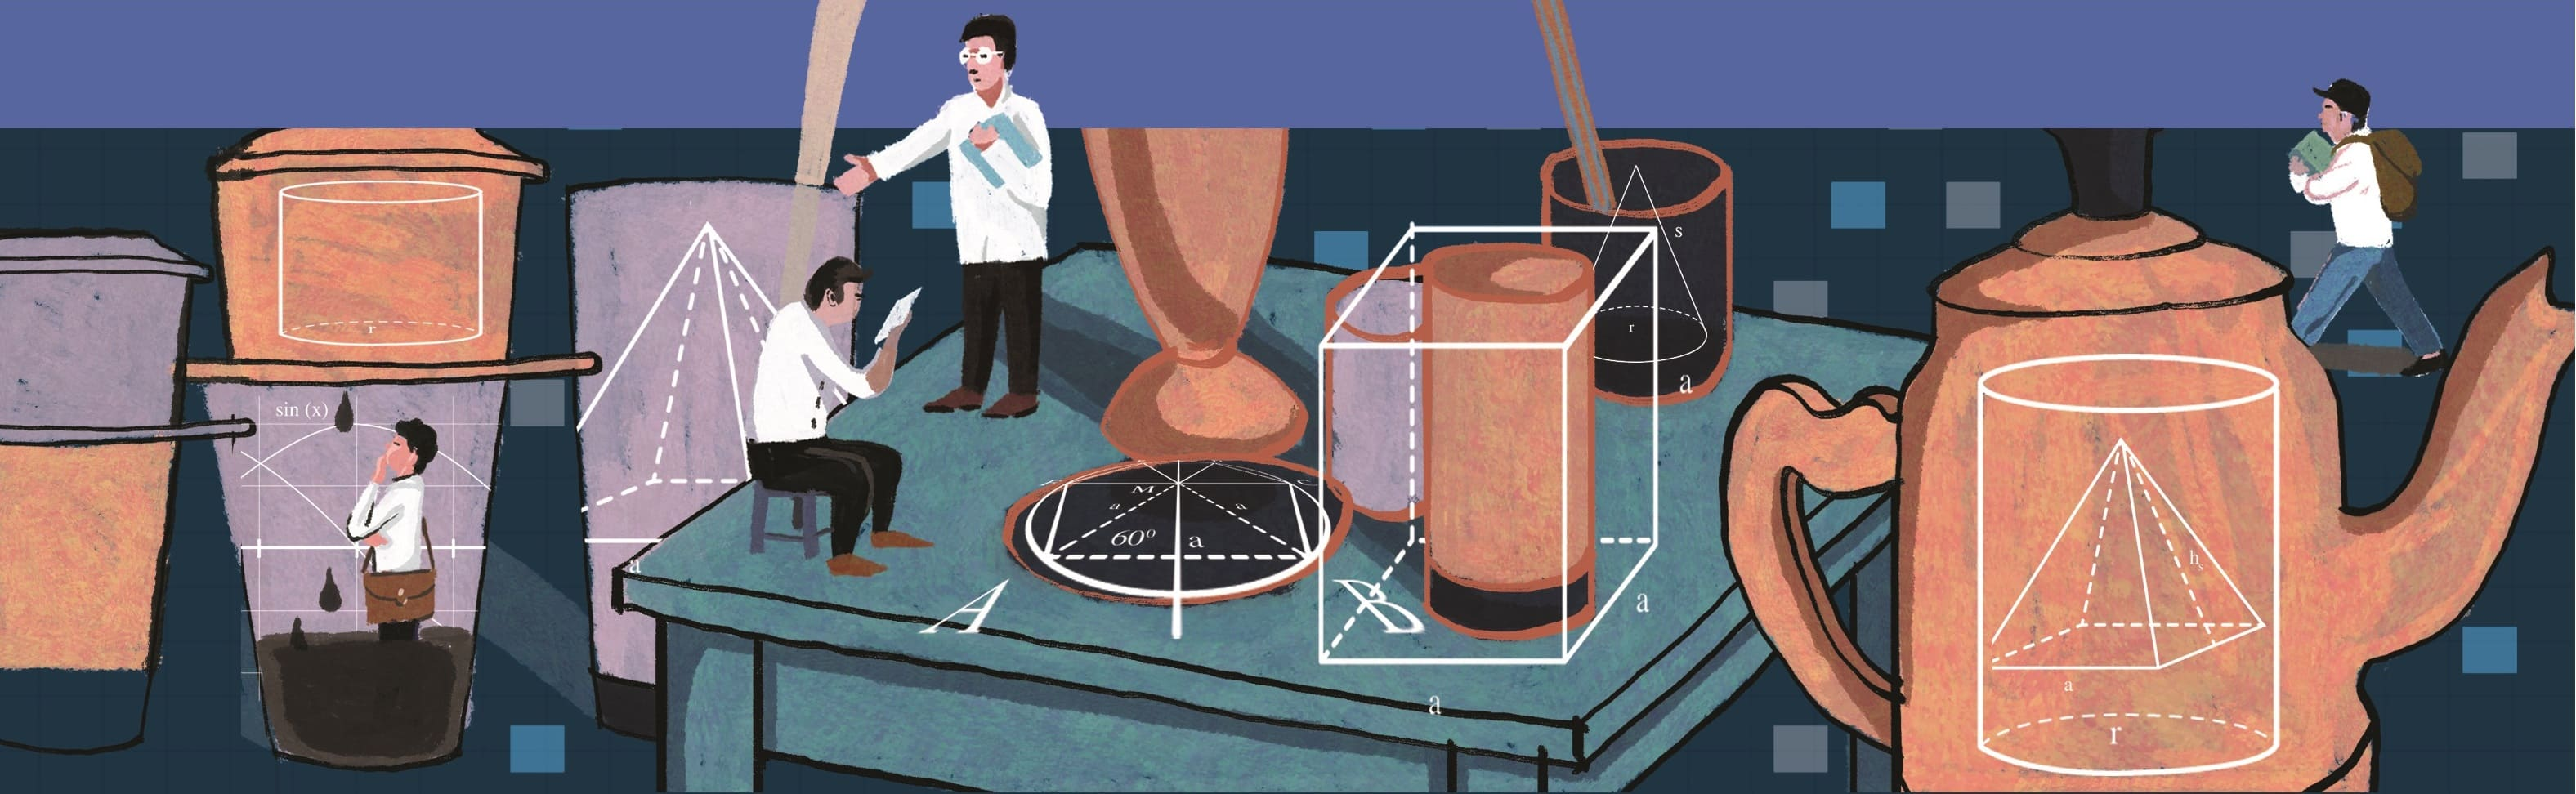
\includegraphics[width=19.3cm]{../bannerquantoan}}}
\AddToShipoutPicture*{\put(132,550){
\includegraphics[scale=1]{../tieude2.pdf}}}
\centering
\endgroup
\vspace*{160pt}

\begin{multicols}{2}
	Richard Feynman ($1918-1988$, Mỹ) nổi tiếng là người trung thực không khoan nhượng và đam mê đến tận cùng. Về tính trung thực, người ta hay nhắc đến vụ ông trình diễn trực tiếp trên TV một ``thí nghiệm nhỏ", bỏ vòng cao su vào cốc nước đá, minh chứng rằng cao su mất tính đàn hồi ở nhiệt độ thấp, qua đó chỉ ra nguyên nhân dẫn đến thảm họa tàu vũ trụ con thoi ``Challenger", vạch trần chiến dịch tung hỏa mù của NASA về nguyên nhân của thảm họa này. Để công bố với người dân Mỹ sự thật ấy, Feynman đã phải vượt qua sức ép khủng khiếp từ các cơ quan công quyền Mỹ, trong đó có CIA và NASA. 
	\vskip 0.1cm
	Feynman lắm đam mê. Đam mê vật lý, Feynman nhận giải Nobel Vật lý năm $1965$. Đam mê chơi trống, vở ba--lê do ông đệm trống nhận giải nhất trong cuộc thi ba--lê toàn nước Mỹ và giải nhì trong cuộc thi quốc tế tại Paris. Đam mê vẽ, ông đã có triển lãm tranh riêng. Không rõ ông biết những ngôn ngữ nào, chỉ biết thăm Brazil ông dạy bằng tiếng Bồ, thăm Nhật ông giao du bằng tiếng Nhật. Rồi có lần bạn bè định ``cho ông một vố", họ nhờ một cô Hoa kiều đón tiếp ông bằng tiếng Trung, Feynman đáp lại và cô ấy kêu trời, vì ông nói tiếng Quảng Đông, còn cô chỉ nói tiếng Bắc Kinh. Rất nhiều ``đam mê" kiểu như vậy được kể trong cuốn ``Feynman, chuyện thật như đùa" (NXB Trẻ) và hầu như tất cả đều có kết cục mỹ mãn, kiểu như giải Nobel. Có thể bạn nghĩ chắc ông này ``con nhà nòi", học ``trường quốc tế" từ nhỏ! Xin thưa, bố của Feynman là người bán rong bán quần áo, còn mẹ thì nội trợ. 
	\begin{figure}[H]
		\vspace*{-5pt}
		\centering
		\captionsetup{labelformat= empty, justification=centering}
		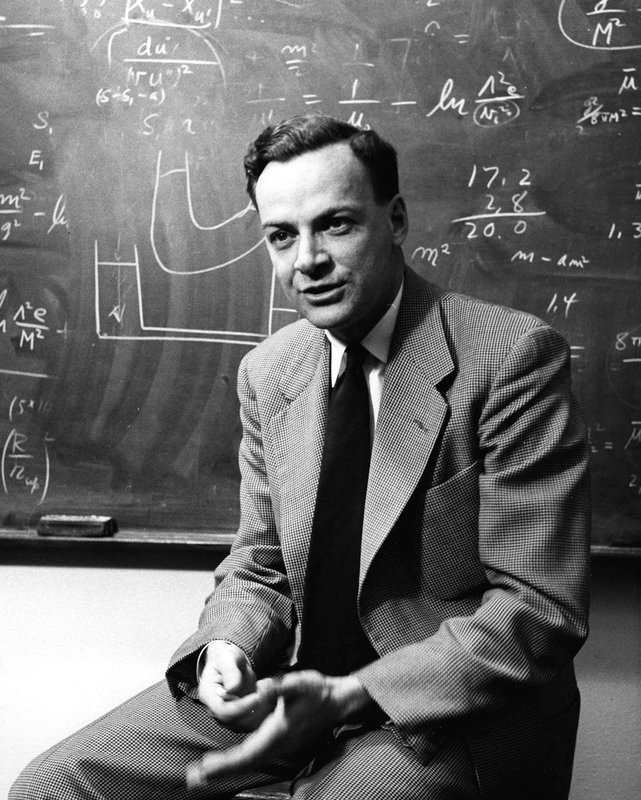
\includegraphics[width= 1\linewidth]{1a}
		\caption{\small\textit{\color{quantoan}Richard Feynman (ảnh từ bộ sưu tập của Viện Công nghệ California -- CalTech).}}
		\vspace*{-10pt}
	\end{figure}
	Ông chơi trống bongo cực giỏi, nhưng chưa bao giờ học nhạc lý. Ông vốn vẽ rất kém, tự nhận chẳng thể vẽ nổi cái gì ngoại trừ cái kim tự tháp chỉ gồm mấy đường thẳng. Để học vẽ, Feynman ``đổi công" với một họa sỹ: ông dạy vật lý cho họa sỹ còn họa sỹ dạy vẽ cho ông. Hãy tưởng tượng một giáo sư nổi tiếng thế giới ngồi trong lớp vẽ cùng các cháu $8-9$ tuổi học cách gọt bút chì. Đam mê như thế chỉ có ở Feynman. Và, với ông đam mê chính là nguồn cội của thành công, chứ chẳng phải ``con nhà nòi" hay ``trường quốc tế" nào cả. Tiền bạc và chứng chỉ đầy người, mà không đam mê gì, thì làm sao có thành quả! 
	\begin{figure}[H]
		\vspace*{-5pt}
		\centering
		\captionsetup{labelformat= empty, justification=centering}
		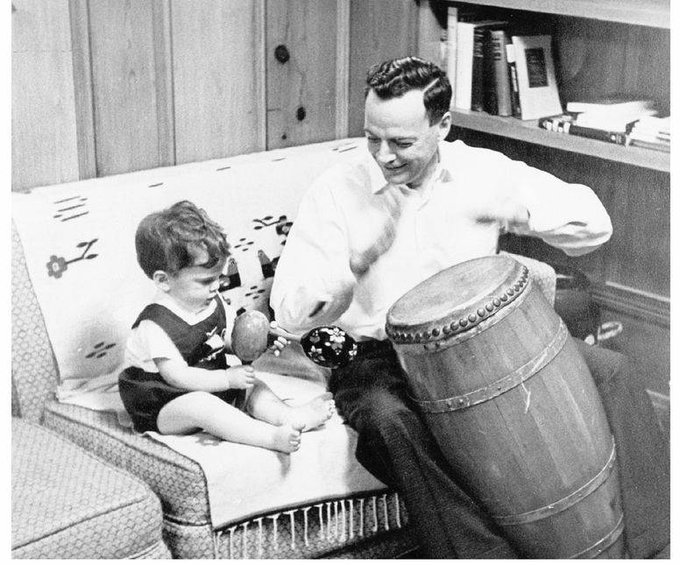
\includegraphics[width= 1\linewidth]{2a}
		\caption{\small\textit{\color{quantoan}Feynman chơi trống bên con trai (ảnh từ Internet).}}
		\vspace*{-10pt}
	\end{figure}
	Duy có đam mê cuối cùng, Feynman đã không kịp nhìn thấy những gì mình muốn, trước khi về cõi vĩnh hằng. Đó là ``Cuộc phiêu lưu cuối cùng của Feynman"\footnote[2]{\color{quantoan}Xem thêm: Cuộc phiêu lưu cuối cùng của Feynman, in lần $2$, NXB Trẻ, $2023$.}. Cuộc phiêu lưu khởi đầu bằng một con tem có xuất xứ từ một nơi gọi là Tannu Tuva, mà Feynman có được từ khi còn nhỏ. Cái tên ``Tuva" xa lạ nằm yên trong đầu Feynman, cho đến một ngày hè $1977$ nó trở thành mục tiêu cho ``cuộc phiêu lưu" kéo dài hơn $10$ năm cuối của cuộc đời ông. Tôi cược là nhiều bạn chưa biết Tuva là địa danh nào và ở đâu. Để đỡ tra cứu, xin ``bật mí" ngay: đó là tên một quốc gia nhỏ nằm giáp phía Tây Bắc của Mông Cổ, vốn độc lập, nhưng đã sáp nhập vào Liên Xô cũ (và Nga ngày nay). Thủ đô của Tuva là Kyzyl. Tuva có gì đặc biệt mà khiến Feynman mê mệt đến vậy?
	\vskip 0.1cm
	Bạn có biết đâu là trọng tâm của châu Á (lục địa thôi chứ không tính các đảo)? Lấy tấm bìa cứng phẳng, vẽ lên đó bản đồ châu Á, cắt theo đường biên để được miếng bìa hình châu Á lục địa. Dùng một chiếc bút đầu nhọn chống phía dưới tấm bìa, di di đầu bút, để tìm vị trí mà tấm bìa nằm cân bằng trên chiếc bút thẳng đứng. Vị trí đó rơi vào Kyzyl, trọng tâm của châu Á. Tất nhiên, các nhà khoa học xác định điểm này bằng các phương pháp chính xác hơn, và ngày nay ở Kyzyl có tấm bia lớn khẳng định vị trí đặc biệt của thành phố này. Nhưng, chỉ chừng ấy thì không đủ để Feynman mất tới cả chục năm tìm cách tới thăm Tuva.
	\begin{figure}[H]
		\vspace*{-5pt}
		\centering
		\captionsetup{labelformat= empty, justification=centering}
		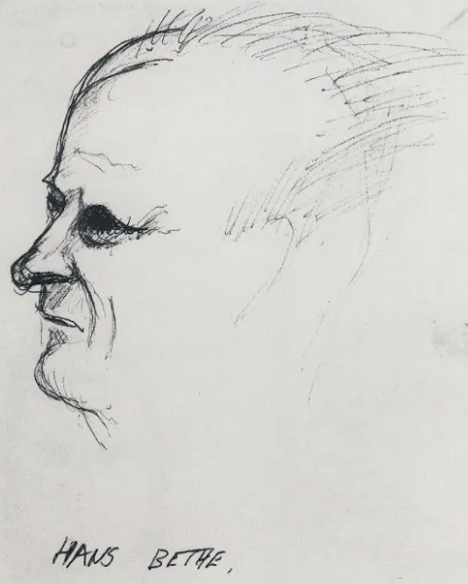
\includegraphics[width= 1\linewidth]{3a}
		\caption{\small\textit{\color{quantoan}Feyman vẽ Hans Bethe (giải Nobel Vật lý $1967$).}}
		\vspace*{-10pt}
	\end{figure}
	Cái chính là ở quốc gia tí xíu bao bọc bởi những dãy núi cao ấy, thời gian gần như ngừng trôi: tất cả vẫn nguyên sơ như $500$ hay $1000$ năm trước. Thảo nguyên hoang dại. Những đàn tuần lộc hay bò Tây Tạng cũng dường như hoang dại. Cuộc sống du mục không thể tự nhiên hơn. Một nền văn hóa xa xưa và kỳ thú với kiểu hát hai giọng chỉ có ở Tuva, với thứ văn tự không thể tìm thấy trong bất cứ tự điển nào, với các tập tục rất lạ điều hành bởi các tù trưởng uy nghi và bí ẩn v.v. Tiếc là ít người biết Tuva, chứ không, người ta đã gọi quốc gia này là ``Thảo nguyên Xanh" cuối cùng của hành tinh Trái Đất (như Congo là Hành tinh Xanh cuối cùng). Đam mê Tuva, Feynman tìm đọc mọi tài liệu về Tuva, tìm hiểu văn tự Tuva, học cách hát của dân du mục Tuva, ăn mặc và trang trí như tù trưởng Tuva \ldots Và, nhất là, ông tìm mọi cách để có thể đến thăm Tuva.
	\vskip 0.1cm
	Đó là thời Chiến tranh Lạnh, lại nghe nói, gần Tuva có một cơ sở nghiên cứu bom nguyên tử, nên nơi đây là ``vùng cấm" với khách du lịch, nhất là khách nước ngoài. Thực ra, Viện Hàn lâm Khoa học Liên Xô sẵn sàng mời Feynman sang Moscow  đọc bài giảng rồi đi ``tham quan Kyzyl" theo kiểu mặc com--lê ở khách sạn có người bảo vệ v.v. Nhưng Feynman không thích như vậy, mà muốn tự mình mang ba--lô đến thảo nguyên, ngủ lều, uống sữa tuần lộc và hát hai giọng cùng dân bản xứ. Ấy thế cho nên ông mất cả chục năm tìm kiếm một giấy mời như mình muốn. Và, đầu tháng Ba $1988$, một giấy mời như thế đã gửi đến địa chỉ của Feynman, chỉ tiếc là hai tuần trước đó, vào ngày $15$ tháng Hai, ông đã ra đi mãi mãi, nên chỉ có thể trải nghiệm ``Cuộc phiêu lưu cuối cùng" của mình trong tâm trí và trái tim của những người ở lại. Không rõ, ở Thế giới bên kia Feynman đang đam mê gì?
	\begin{figure}[H]
		\vspace*{-5pt}
		\centering
		\captionsetup{labelformat= empty, justification=centering}
		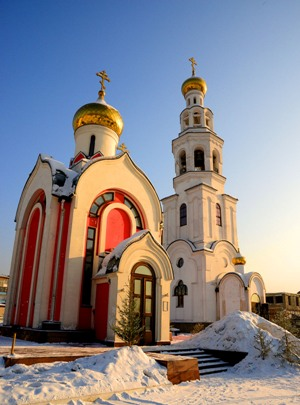
\includegraphics[width= 1\linewidth]{4a}
		\caption{\small\textit{\color{quantoan}Nhà thờ Phục sinh ở Kyzyl, Tuva (ảnh từ Internet).}}
%		\vspace*{-10pt}
	\end{figure}
\end{multicols}
\vspace*{-10pt}
{\rule{1\linewidth}{0.1pt}}
\vskip 0.25cm
\centerline{\LARGE\textbf{\color{quantoan}LỜI GIẢI, ĐÁP ÁN}}
\begin{multicols}{2}
	\textbf{\color{quantoan}Tìm ra người đặc biệt}
	\vskip 0.1cm
	$a)$ Ta sẽ chỉ ra chiến thuật dẫn tới mục đích phát hiện ra nhân viên $Z$ sau đúng $(n-1)$ câu hỏi. Đầu tiên, Xuân Phong chọn hai người tuỳ ý là $A$ và $B$. Xuân Phong hỏi nhân viên $A$ câu hỏi: ``Anh có biết $B$  không?" Nếu câu trả lời là ``Có" thì $B$ không phải là $Z$. Còn nếu câu trả lời là ``Không" thì $A$ không phải là $Z$. Như vậy, với một câu hỏi được đưa ra thì một người sẽ loại ra, tiếp theo không cần phải hỏi anh ta và cũng không cần hỏi về anh ta nữa. Cứ tiếp tục kiểu như vậy, ta loại đi $(n-1)$ người sau khi hỏi $(n-1)$ câu hỏi. Còn lại đúng một người. Anh ta chính là nhân viên $Z$.
	\vskip 0.1cm
	$b)$ Ta sẽ chỉ ra Xuân Phong phải hỏi không ít hơn $(n-1)$ câu hỏi. 
	\vskip 0.1cm
	Giả sử tại một bước nào đó của cuộc điều tra, Xuân Phong hỏi một nhân viên $A$, anh ta có biết nhân viên $B$ hay không. Trong trường hợp câu trả lời ``có", ta sẽ coi $B$ là được đánh dấu, còn trong trường hợp câu trả lời là ``không", ta sẽ coi $A$ là được đánh~dấu.
	\vskip 0.1cm
	\hfill (\textit{Xem tiếp trang} $64$)
\end{multicols}
	\newpage
%
%	\thispagestyle{empty}
%	\begingroup 
%	\AddToShipoutPicture*{\put(0,0){\includegraphics[width=19.45cm]{QC}}}
%	\centering
%	\vspace*{0cm}
%	\endgroup
%	\newpage	 
%	\pagestyle{empty}
%
%	\setcounter{figure}{0}
%	\thispagestyle{toancuabinone}
\pagestyle{toancuabi}
\everymath{\color{toancuabi}}
\blfootnote{$^*$\color{toancuabi}Nguồn: Câu lạc bộ Toán học Unicorn (UMC)}
\graphicspath{{../toancuabi/pic/}}
\begingroup
\AddToShipoutPicture*{\put(0,616){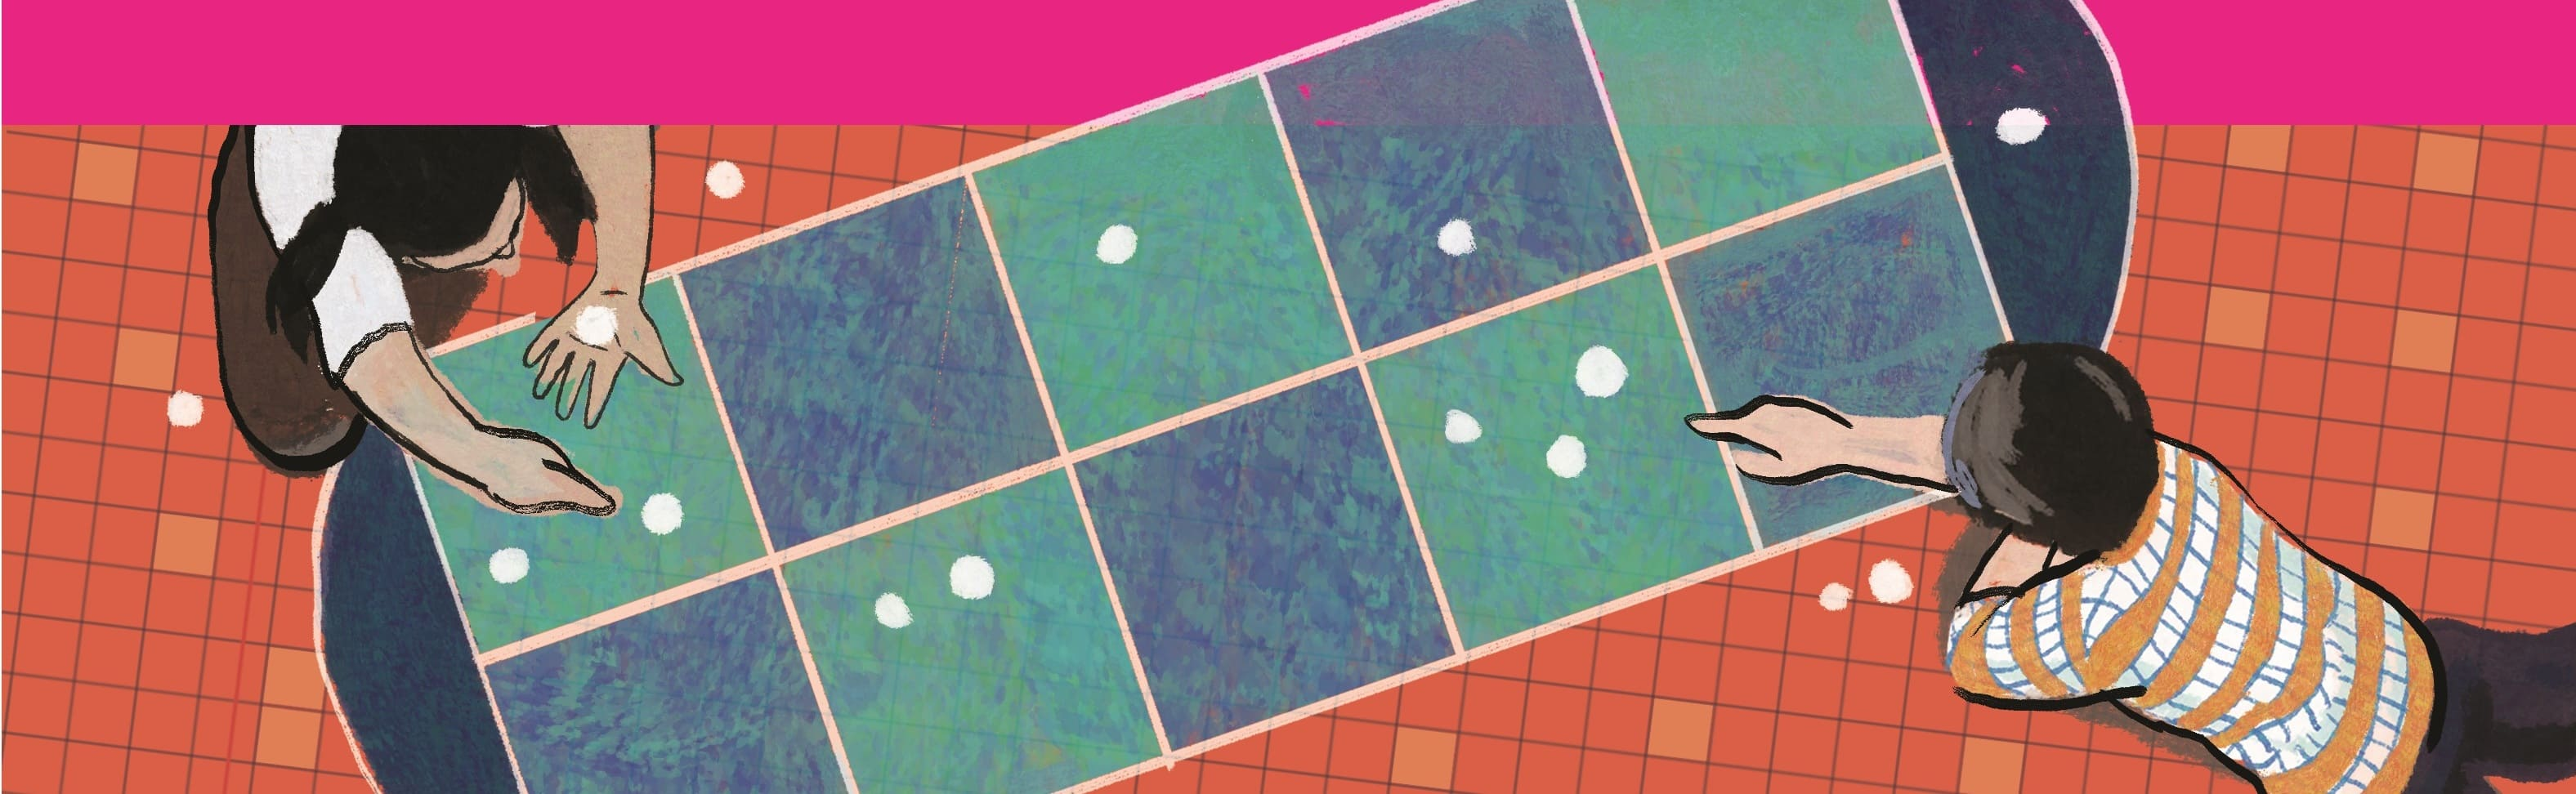
\includegraphics[width=19.3cm]{../bannertoancuabi}}}  
\AddToShipoutPicture*{\put(62,512){
\includegraphics[scale=1]{../tieude1.pdf}}}  
\centering
\endgroup
\vspace*{195pt} 

\definecolor{bulgarianrose}{rgb}{0.28, 0.02, 0.03}
\begin{multicols}{2}
	Trong số này, tạp chí Pi tiếp tục giới thiệu đến với bạn đọc đề thi tuyển sinh năm $2023-2024$ dành cho các bạn học sinh lớp $5$. Các bạn có thể thử sức làm của mình trong khoảng thời gian $90$ phút.
	\vskip 0.1cm
	\textbf{\color{toancuabi}Bài $\pmb1$.} 
	Dựa vào quy luật, hãy cho biết có bao nhiêu dấu thăng trong hình thứ tám của dãy hình sau.
	\begin{figure}[H]
		\vspace*{-5pt}
		\centering
		\captionsetup{labelformat= empty, justification=centering}
		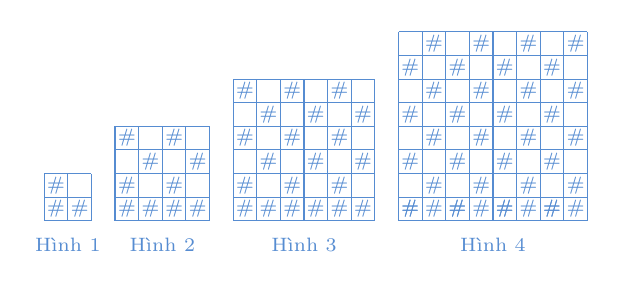
\begin{tikzpicture}[cackithi,scale=0.3,node font=\scriptsize]
			\draw (0,0) grid (2,2);	
			\draw (3,0) grid (7,4);
			\draw (8,0) grid (14,6);
			\draw (15,0) grid (23,8);
			\draw (0.5,0.5) node {$\#$};
			\draw (1.5,0.5) node {$\#$};
			\draw (0.5,1.5) node {$\#$};
			\draw (3.5,0.5) node {$\#$};
			\draw (4.5,0.5) node {$\#$};
			\draw (5.5,0.5) node {$\#$};
			\draw (6.5,0.5) node {$\#$};
			\draw (3.5,1.5) node {$\#$};
			\draw (5.5,1.5) node {$\#$};
			\draw (4.5,2.5) node {$\#$};
			\draw (6.5,2.5) node {$\#$};
			\draw (3.5,3.5) node {$\#$};
			\draw (5.5,3.5) node {$\#$};
			\draw (8.5,0.5) node {$\#$};
			\draw (9.5,0.5) node {$\#$};
			\draw (10.5,0.5) node {$\#$};
			\draw (11.5,0.5) node {$\#$};
			\draw (12.5,0.5) node {$\#$};
			\draw (13.5,0.5) node {$\#$};
			\draw (8.5,1.5) node {$\#$};
			\draw (10.5,1.5) node {$\#$};
			\draw (12.5,1.5) node {$\#$};
			\draw (9.5,2.5) node {$\#$};
			\draw (11.5,2.5) node {$\#$};
			\draw (13.5,2.5) node {$\#$};
			\draw (8.5,3.5) node {$\#$};
			\draw (10.5,3.5) node {$\#$};
			\draw (12.5,3.5) node {$\#$};
			\draw (9.5,4.5) node {$\#$};
			\draw (11.5,4.5) node {$\#$};
			\draw (13.5,4.5) node {$\#$};
			\draw (8.5,5.5) node {$\#$};
			\draw (10.5,5.5) node {$\#$};
			\draw (12.5,5.5) node {$\#$};
			\draw (15.5,0.5) node {$\#$};
			\draw (16.5,0.5) node {$\#$};
			\draw (17.5,0.5) node {$\#$};
			\draw (18.5,0.5) node {$\#$};
			\draw (19.5,0.5) node {$\#$};
			\draw (20.5,0.5) node {$\#$};
			\draw (21.5,0.5) node {$\#$};
			\draw (22.5,0.5) node {$\#$};
			\draw (15.5,0.5) node {$\#$};
			\draw (17.5,0.5) node {$\#$};
			\draw (19.5,0.5) node {$\#$};
			\draw (21.5,0.5) node {$\#$};
			\draw (16.5,1.5) node {$\#$};
			\draw (18.5,1.5) node {$\#$};
			\draw (20.5,1.5) node {$\#$};
			\draw (22.5,1.5) node {$\#$};
			\draw (15.5,2.5) node {$\#$};
			\draw (17.5,2.5) node {$\#$};
			\draw (19.5,2.5) node {$\#$};
			\draw (21.5,2.5) node {$\#$};
			\draw (16.5,3.5) node {$\#$};
			\draw (18.5,3.5) node {$\#$};
			\draw (20.5,3.5) node {$\#$};
			\draw (22.5,3.5) node {$\#$};
			\draw (15.5,4.5) node {$\#$};
			\draw (17.5,4.5) node {$\#$};
			\draw (19.5,4.5) node {$\#$};
			\draw (21.5,4.5) node {$\#$};
			\draw (16.5,5.5) node {$\#$};
			\draw (18.5,5.5) node {$\#$};
			\draw (20.5,5.5) node {$\#$};
			\draw (22.5,5.5) node {$\#$};
			\draw (15.5,6.5) node {$\#$};
			\draw (17.5,6.5) node {$\#$};
			\draw (19.5,6.5) node {$\#$};
			\draw (21.5,6.5) node {$\#$};
			\draw (16.5,7.5) node {$\#$};
			\draw (18.5,7.5) node {$\#$};
			\draw (20.5,7.5) node {$\#$};
			\draw (22.5,7.5) node {$\#$};
			\draw (1,-1) node {Hình $1$};
			\draw (5,-1) node {Hình $2$};
			\draw (11,-1) node {Hình $3$};
			\draw (19,-1) node {Hình $4$};
		\end{tikzpicture}
		\vspace*{-15pt}
	\end{figure}
	\textbf{\color{toancuabi}Bài $\pmb2$.} Bạn Tâm xếp các số $0, 0, 1, 1, 2, 2, 2, 3$ vào các ô vuông trong hình dưới đây (mỗi ô một số) để tạo thành phép trừ của hai số có $4$ chữ số. Hỏi hiệu nhận được lớn nhất có thể là bao nhiêu? 
	\vskip 0.1cm
	Chú ý: \textit{một số có bốn chữ số không được bắt đầu bằng số $0$.}
	\begin{figure}[H]
		\vspace*{-5pt}
		\centering
		\captionsetup{labelformat= empty, justification=centering}
		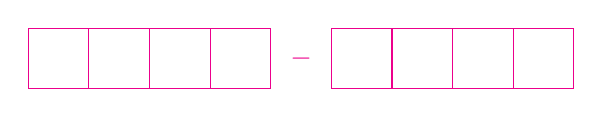
\begin{tikzpicture}[toancuabi,scale=0.77]
			\draw (0,0) grid (4,1);
			\draw (4.5,0.5) node {$-$};
			\draw (5,0) grid (9,1);
		\end{tikzpicture}
		\vspace*{-10pt}
	\end{figure}
	\textbf{\color{toancuabi}Bài $\pmb3$.} Diện tích của hình được tô đậm bên dưới bằng bao nhiêu?
	\begin{figure}[H]
		\vspace*{5pt}
		\centering
		\captionsetup{labelformat= empty, justification=centering}
		\definecolor{zzttqq}{rgb}{0.6,0.2,0.}
		\begin{tikzpicture}[toancuabi, scale=0.9]
			\fill[color=cackithi,fill=cackithi!40] (1.,0.) -- (2.,5.) -- (3.,0.) -- cycle;
			\fill[color=zzttqq,fill=cackithi!40] (1.,0.) -- (4.,5.) -- (3.,0.) -- (0.,5.) -- cycle;
			\draw  (1.,0.)-- (2.,5.);
			\draw  (2.,5.)-- (3.,0.);
			\draw  (3.,0.)-- (1.,0.);
			\draw  (1.,0.)-- (4.,5.);
			\draw  (4.,5.)-- (3.,0.);
			\draw  (3.,0.)-- (0.,5.);
			\draw  (0.,5.)-- (1.,0.);
			\draw[dashed]  (-1.,5.)-- (5.,5.);
			\draw[dashed]  (-1.,2.5)-- (5.,2.5);
			\draw[dashed]  (-1.,0.)-- (5.,0.);
			\draw[-stealth]  (4.5,5.)-- (4.5,2.5);
			\draw[-stealth]  (4.5,2.5)-- (4.5,0.);
			\draw[-stealth]  (1,-0.4)-- (3.,-0.4);
			
			\draw[-stealth]  (4.5,2.5) -- (4.5,5.);
			\draw[-stealth]  (4.5,0.) -- (4.5,2.5);
			\draw[-stealth]  (3.,-0.4) -- (1,-0.4);
			\draw[color=black] (4.21498164902576,3.87946061896495) node {$5$};
			\draw[color=black] (4.143071467449243,1.3626042637868525) node {$5$};
			\draw[color=black] (2.039698656336115,-0.709930933849792) node {$4$};
		\end{tikzpicture}
		\vspace*{-10pt}
	\end{figure}
	\textbf{\color{toancuabi}Bài $\pmb4$.} Trong bảng ô vuông cỡ $4\times 4$ có điền các số khác $0$ sao cho tích của $4$ số trong mỗi hàng, mỗi cột đều bằng nhau. Cho biết các số trong $9$ ô như hình vẽ, hỏi số ở ô có dấu $*$ bằng bao nhiêu?
	\begin{figure}[H]
		\vspace*{-5pt}
		\centering
		\captionsetup{labelformat= empty, justification=centering}
		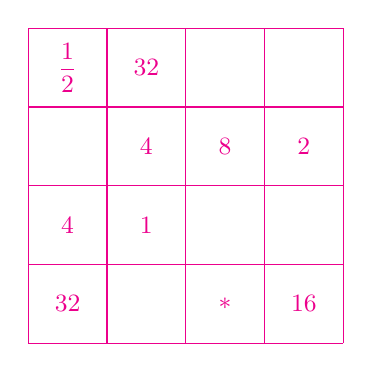
\begin{tikzpicture}[toancuabi, node font=\small]
			\draw (0,0) grid (4,4);
			\draw (0.5,0.5) node {$32$};
			\draw (0.5,1.5) node {$4$};
			\draw (0.5,3.5) node {$\dfrac{1}{2}$};
			\draw (1.5,1.5) node {$1$};
			\draw (1.5,2.5) node {$4$};
			\draw (1.5,3.5) node {$32$};
			\draw (2.5,0.5) node {$*$};
			\draw (3.5,0.5) node {$16$};
			\draw (2.5,2.5) node {$8$};
			\draw (3.5,2.5) node {$2$};
		\end{tikzpicture}
		\vspace*{-5pt}
	\end{figure}
	\textbf{\color{toancuabi}Bài $\pmb5$.} Khu vườn của gia đình Tâm được minh họa bằng hình chữ nhật trong hình dưới đây. Biết rằng khu vườn có diện tích $120 \,m^2$ và được chia thành ba luống hình chữ nhật. Phần trồng hoa rộng $2\,m$, diện tích $20 \,m^2$, phần trồng dâu rộng $3\, m$. Hỏi diện tích phần trồng rau là bao nhiêu?
	\begin{figure}[H]
		\vspace*{-5pt}
		\centering
		\captionsetup{labelformat= empty, justification=centering}
		\begin{tikzpicture}[scale=0.4,toancuabi]
			\draw (0,0) rectangle (12,10);
			\draw (2,0) -- (2,10) (2,3) -- (12,3);
			\draw (1,10) node[below] {$2\,m$};
			\draw (1,5) node {Hoa};
			\draw (7,1.5) node {Dâu};
			\draw (7,6.5) node {Rau};
			\draw (12,1.5) node[right] {$3\,m$};
		\end{tikzpicture}
		\vspace*{-5pt}
	\end{figure}
	\textbf{\color{toancuabi}Bài $\pmb6$.} Ba bạn An, Bình, Chi chia đều nhau $30$ chiếc kẹo. An ăn một số chiếc kẹo; Bình ăn một số kẹo bằng với số kẹo mà An còn; Chi ăn số kẹo bằng với tổng số kẹo mà An và Bình đã ăn. Hỏi còn lại bao nhiêu chiếc kẹo?
	\vskip 0.1cm
	\textbf{\color{toancuabi}Bài $\pmb7$.} Một bác nông dân chở một xe ô tô quất cảnh ra chợ Tết để bán. Sau khi bán hết cây quất cuối cùng với giá $230$ nghìn đồng, bác tính nhẩm lại thấy mình đã bán số cây quất với giá trung bình là $245$ nghìn đồng/cây. Nhưng người mua cây quất cuối quay trở lại và chỉ cho bác thấy cành quất bị rụng quá nhiều lá, nên ông ta chỉ đồng ý mua với giá $158$ nghìn đồng. Bác chấp thuận và bán cây quất đó. Khi nhẩm tính lại, bác nông dân thấy giá trung bình của xe quất bây giờ là $242$ nghìn đồng. Hỏi bác đã bán được bao nhiêu cây quất?
	\vskip 0.1cm
	\columnbreak
	\textbf{\color{toancuabi}Bài $\pmb8$.} Có bao nhiêu cách xếp $5$ viên bi giống hệt nhau vào các ô hình vuông ở hình vẽ sau sao cho mỗi ô có không quá $1$ viên bi và không có $2$ viên bi nào trên cùng $1$ hàng hoặc $1$ cột?
	\begin{figure}[H]
		\vspace*{-10pt}
		\centering
		\captionsetup{labelformat= empty, justification=centering}
		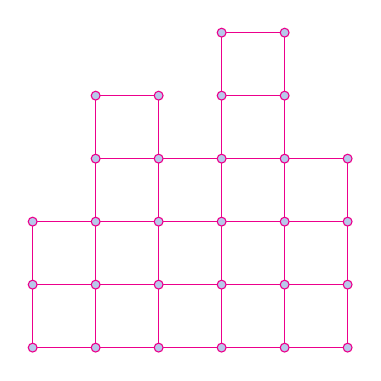
\begin{tikzpicture}[toancuabi,scale=0.8]
			\draw  (0.,1.)-- (5.,1.);
			\draw  (5.,1.)-- (5.,4.);
			\draw  (5.,4.)-- (1.,4.);
			\draw  (1.,4.)-- (1.,3.);
			\draw  (1.,3.)-- (0.,3.);
			\draw  (0.,3.)-- (0.,1.);
			\draw  (1.,1.)-- (1.,3.);
			\draw  (1.,2.)-- (5.,2.);
			\draw  (5.,3.)-- (1.,3.);
			\draw  (1.,4.)-- (1.,5.);
			\draw  (1.,5.)-- (2.,5.);
			\draw  (2.,5.)-- (2.,1.);
			\draw  (3.,1.)-- (3.,6.);
			\draw  (3.,6.)-- (4.,6.);
			\draw  (4.,6.)-- (4.,1.);
			\draw  (0.,2.)-- (1.,2.);
			\draw  (3.,5.)-- (4.,5.);
			
			\draw [fill=cackithi!40] (0.,1.) circle (2.0pt);
			\draw [fill=cackithi!40] (5.,1.) circle (2.0pt);
			\draw [fill=cackithi!40] (5.,4.) circle (2.0pt);
			\draw [fill=cackithi!40] (1.,4.) circle (2.0pt);
			\draw [fill=cackithi!40] (1.,3.) circle (2.0pt);
			\draw [fill=cackithi!40] (0.,3.) circle (2.0pt);
			\draw [fill=cackithi!40] (1.,1.) circle (2.0pt);
			\draw [fill=cackithi!40] (1.,2.) circle (2.0pt);
			\draw [fill=cackithi!40] (5.,2.) circle (2.0pt);
			\draw [fill=cackithi!40] (5.,3.) circle (2.0pt);
			\draw [fill=cackithi!40] (1.,5.) circle (2.0pt);
			\draw [fill=cackithi!40] (2.,5.) circle (2.0pt);
			\draw [fill=cackithi!40] (2.,1.) circle (2.0pt);
			\draw [fill=cackithi!40] (3.,1.) circle (2.0pt);
			\draw [fill=cackithi!40] (3.,6.) circle (2.0pt);
			\draw [fill=cackithi!40] (4.,6.) circle (2.0pt);
			\draw [fill=cackithi!40] (4.,1.) circle (2.0pt);
			\draw [fill=cackithi!40] (2.,4.) circle (2.0pt);
			\draw [fill=cackithi!40] (3.,4.) circle (2.0pt);
			\draw [fill=cackithi!40] (4.,4.) circle (2.0pt);
			\draw [fill=cackithi!40] (4.,5.) circle (2.0pt);
			\draw [fill=cackithi!40] (3.,5.) circle (2.0pt);
			\draw [fill=cackithi!40] (4.,3.) circle (2.0pt);
			\draw [fill=cackithi!40] (3.,3.) circle (2.0pt);
			\draw [fill=cackithi!40] (2.,3.) circle (2.0pt);
			\draw [fill=cackithi!40] (2.,2.) circle (2.0pt);
			\draw [fill=cackithi!40] (3.,2.) circle (2.0pt);
			\draw [fill=cackithi!40] (4.,2.) circle (2.0pt);
			\draw [fill=cackithi!40] (0.,2.) circle (2.0pt);
		\end{tikzpicture}
		\vspace*{-5pt}
	\end{figure}
	\textbf{\color{toancuabi}Bài $\pmb9$.} Mỗi ô trong hình bên được điền một số sao cho: số được ghi trong mỗi ô ở $3$ hàng trên cùng bằng tổng $2$ số ở hai ô ngay bên dưới nó. 
	Cho biết trước $3$ số như trong hình vẽ, hỏi số nào phải được điền vào ô có chữ $x$?
	\begin{figure}[H]
		\vspace*{-5pt}
		\centering
		\captionsetup{labelformat= empty, justification=centering}
		\begin{tikzpicture}[xscale=2,scale=0.8,toancuabi]
			\draw (0,0) grid (4,1);
			\draw (1,2) grid (3,3);
			\draw (0.5,1) rectangle (3.5,2);
			\draw (1.5,3) rectangle (2.5,4);
			\draw (1.5,1) --(1.5,2) (2.5,1) --(2.5,2);
			\draw (0.5,0.5) node {$10$};
			\draw (3.5,0.5) node {$12$};
			\draw (2,1.5) node {$x$};
			\draw (2,3.5) node {$100$};
		\end{tikzpicture}
		\vspace*{-5pt}
	\end{figure}
	\textbf{\color{toancuabi}Bài $\pmb{10}$.} Sau khi sạc điện thoại di động, bạn Kiên nhận ra mình đã quên mã PIN (mã gồm $4$ chữ số). Kiên nhớ là mã PIN bắt đầu bằng số $1$, kết thúc bằng số $3$ và các chữ số trong mã đều khác nhau.
	Có bao nhiêu số khác nhau cho mã PIN của Kiên?
	\end{multicols}
	\newpage
	\begin{multicols}{2}
	\textbf{\color{toancuabi}Đáp án}
	\vskip 0.1cm
	\textbf{\color{toancuabi}Bài $\pmb1$.} Nhận thấy Hình thứ $n$ trong dãy là một hình vuông có các đặc điểm sau:
	\vskip 0.1cm
	-- Cạnh hình vuông có kích thước là: $2\times n$;
	\vskip 0.1cm
	-- Hàng cuối có $2\times n$ dấu $\#$ và các hàng còn lại có $n$ dấu $\#$.
	\vskip 0.1cm
	Như vậy số dấu $\#$ trong Hình thứ $8$ là:
	\begin{align*}
		15\times 8 + 16 = 136. 
	\end{align*}
	\textbf{\color{toancuabi}Bài $\pmb2$.} Để hiệu nhận được là lớn nhất thì số bị trừ là số lớn nhất có $4$ chữ số và số trừ sẽ nhỏ nhất có $4$ chữ số tạo từ các số đã cho.
	\vskip 0.1cm
	Do đó số bị trừ là $3222$ và số trừ là $1001$ và ta có hiệu lớn nhất có thể là:
	\begin{align*}
		3222 - 1001 = 2221.
	\end{align*}
	\textbf{\color{toancuabi}Bài $\pmb3$.} Ta viết tên các điểm như trong hình vẽ dưới đây.
	\begin{figure}[H]
		\vspace*{5pt}
		\centering
		\captionsetup{labelformat= empty, justification=centering}
		\definecolor{zzttqq}{rgb}{0.6,0.2,0.}
		\begin{tikzpicture}[toancuabi, scale=0.9]
			\fill[color=cackithi,fill=cackithi!40] (1.,0.) -- (2.,5.) -- (3.,0.) -- cycle;
			\fill[color=zzttqq,fill=cackithi!40] (1.,0.) -- (4.,5.) -- (3.,0.) -- (0.,5.) -- cycle;
			\draw  (1.,0.)-- (2.,5.);
			\draw  (2.,5.)-- (3.,0.);
			\draw  (3.,0.)-- (1.,0.);
			\draw  (1.,0.)-- (4.,5.);
			\draw  (4.,5.)-- (3.,0.);
			\draw  (3.,0.)-- (0.,5.);
			\draw  (0.,5.)-- (1.,0.);
			
			\draw [fill=cackithi!40] (0.5,2.5) circle (2.0pt) node[anchor=north east] {$D$};
			\draw [fill=cackithi!40] (1.5,2.5) circle (2.0pt) node[above] {$E$};
			\draw [fill=cackithi!40] (2.5,2.5) circle (2.0pt) node[above] {$F$};
			\draw [fill=cackithi!40] (3.5,2.5) circle (2.0pt) node[anchor = north west] {$G$};
			\draw [fill=cackithi!40] (4.,5.) circle (2.0pt) node[above] {$C$};
			\draw [fill=cackithi!40] (0.,5.) circle (2.0pt) node[above] {$A$};
			\draw [fill=cackithi!40] (2.,5.) circle (2.0pt) node[above] {$B$};
			\draw [fill=cackithi!40] (1.,0.) circle (2.0pt) node[anchor=north east] {$K$};
			\draw [fill=cackithi!40] (3.,0.) circle (2.0pt) node[anchor = north west] {$H$};
			
			\draw[dashed]  (-1.,5.)-- (5.,5.);
			\draw[dashed]  (-1.,2.5)-- (5.,2.5);
			\draw[dashed]  (-1.,0.)-- (5.,0.);
			\draw[-stealth]  (4.5,5.)-- (4.5,2.5);
			\draw[-stealth]  (4.5,2.5)-- (4.5,0.);
			\draw[-stealth]  (1,-0.4)-- (3.,-0.4);
			
			\draw[-stealth]  (4.5,2.5) -- (4.5,5.);
			\draw[-stealth]  (4.5,0.) -- (4.5,2.5);
			\draw[-stealth]  (3.,-0.4) -- (1,-0.4);
			\draw[color=black] (4.21498164902576,3.87946061896495) node {$5$};
			\draw[color=black] (4.143071467449243,1.3626042637868525) node {$5$};
			\draw[color=black] (2.039698656336115,-0.709930933849792) node {$4$};
		\end{tikzpicture}
		\vspace*{-10pt}
	\end{figure}
	Nhận thấy phần tô đậm có diện tích bằng tổng diện tích của các tam giác sau.
	$BKH,$ $ADE,$ $DEK,$ $CFG$ và $FGH.$
	\vskip 0.1cm
	Tam giác $BKH$ có đáy $KH = 4$ và chiều cao bằng $10$, do đó có diện tích là: \begin{align*}
		\dfrac{1}{2} \times 4 \times 10 = 20.
	\end{align*}
	Các tam giác $ADE$, $DEK$, $CFG$ và $FGH$ có các đáy $DE=EF=FG = 2$ và chiều cao bằng $5$, do đó có cùng diện tích là: 
	\begin{align*}
		\dfrac{1}{2} \times 2\times 5 = 5.
	\end{align*}
	Vậy diện tích của phần tô đậm là:
	\begin{align*}
		20 + 4\times 5 = 40 \text{ (đơn vị diện tích)}
	\end{align*}
	\textbf{\color{toancuabi}Bài $\pmb4$.} Do tích của mỗi hàng và mỗi cột đều bằng nhau nên tích các số của cột thứ $2$ và hàng thứ $4$ bằng nhau. Vì cột $2$ và hàng $4$ chung nhau một ô nên tích của $3$ số còn lại bằng nhau. Từ đó, ta có
	\begin{align*}
		32\times 4\times 1 = 32\times * \times 16.
	\end{align*}
	Giải ra ta được số ở ô có dấu $*$ là $\dfrac{1}{4}$.
	\vskip 0.1cm
	\textbf{\color{toancuabi}Bài $\pmb5$.} Điền tên các đỉnh trong hình như sau.
	\begin{figure}[H]
		\vspace*{-5pt}
		\centering
		\captionsetup{labelformat= empty, justification=centering}
		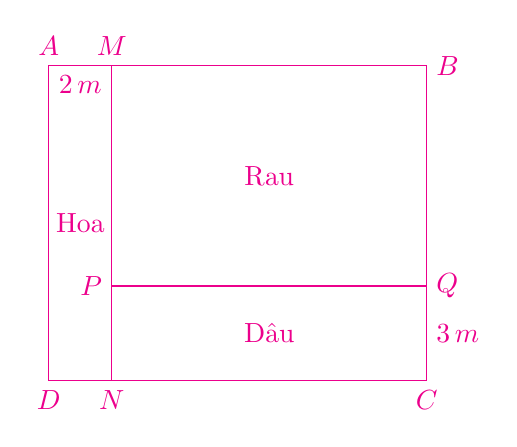
\begin{tikzpicture}[scale=0.4,toancuabi]
			\draw (0,0) rectangle (12,10);
			\draw (2,0) -- (2,10) (2,3) -- (12,3);
			\draw (0,0) node[below] {$D$};
			\draw (2,0) node[below] {$N$};
			\draw (12,0) node[below] {$C$};
			\draw (2,3) node[left] {$P$};
			\draw (12,3) node[right] {$Q$};
			\draw (12,10) node[right] {$B$};
			\draw (2,10) node[above] {$M$};
			\draw (0,10) node[above] {$A$};
			\draw (1,10) node[below] {$2\,m$};
			\draw (1,5) node {Hoa};
			\draw (7,1.5) node {Dâu};
			\draw (7,6.5) node {Rau};
			\draw (12,1.5) node[right] {$3\,m$};
		\end{tikzpicture}
		\vspace*{-10pt}
	\end{figure}
	Phần trồng hoa là hình chữ nhật $AMND$ có diện tích là $20\,m^2$. Hình chữ nhật AMND có cạnh $AM=2\,m$ nên cạnh còn lại $AD=10\,m$.
	\vskip 0.1cm
	Khu vườn là hình chữ nhật $ABCD$ có diện tích $120\, m^2$. Hình chữ nhật $ABCD$ có cạnh $AD=10\,m$ nên cạnh $DC = 12\,m$.
	\vskip 0.1cm
	Ta có
	$DC = 12 = DN + NC = 2 + NC$. Do đó $NC=10$.
	\vskip 0.1cm
	Từ đó, phần trồng dâu là hình chữ nhật $PQCN$ có hai cạnh $NC=10$ và $QC=3$. Do đó diện tích của phần trồng dâu là: $30\,m^2$.
	\vskip 0.1cm
	Vậy diện tích của phần trồng rau là: $120 - 20 - 30 = 70\,m^2$. 
	\vskip 0.1cm
	\textbf{\color{toancuabi}Bài $\pmb6$.}
	Mỗi bạn được chia $30: 3=10$ chiếc kẹo.
	\vskip 0.1cm
	Do Bình ăn một số kẹo bằng với số kẹo mà An còn nên tổng số kẹo mà An và Bình ăn là $10$ chiếc. Vì thế tổng số kẹo mà An, Bình và Chi ăn là $10+10=20$ chiếc. Do vậy, còn lại $30-20=10$ chiếc kẹo.
	\vskip 0.1cm
	\textbf{\color{toancuabi}Bài $\pmb7$.} Gọi số cây quất là $n$. Khi đó tổng tiền bán được của lần bán đầu khi cây cuối có giá $230$ nghìn là $245\times n$ và tổng tiền thu được khi bán cây cuối với giá $158$ nghìn là $242\times n$. Ta thấy chênh lệch giữa giá bán cây cuối ở $2$ lần bằng $3\times n$. Do số tiền chênh lệch giữa hai lần bán là: 
	\begin{align*}
		230-158=72 \text{ nghìn}
	\end{align*}
	nên bác nông dân đã bán được 
	\begin{align*}
		72:3 = 24 \text{ cây quất.}
	\end{align*}
	\textbf{\color{toancuabi}Bài $\pmb8$.} Ta thấy
	Cột $1$ có $2$ cách xếp bi;
	\vskip 0.1cm
	Cột $3$ có $2$ cách xếp bi;
	\vskip 0.1cm
	Cột $5$ có $1$ cách xếp  bi;
	\vskip 0.1cm
	Cột $2$ có $1$ cách xếp  bi;
	\vskip 0.1cm
	Cột $4$ có $1$ cách xếp  bi.
	\vskip 0.1cm
	Do đó, số cách xếp bi là: $2\times 2\times 1\times 1\times 1 = 4$ (cách)
	\vskip 0.1cm
	\textbf{\color{toancuabi}Bài $\pmb9$.} Gọi hai số còn khuyết ở hàng cuối là $a$ và $b$. Do mỗi ô ở hàng trên bằng tổng hai ô ngay bên dưới nên ta điền được các số như sau.
	\begin{figure}[H]
		\vspace*{-5pt}
		\centering
		\captionsetup{labelformat= empty, justification=centering}
		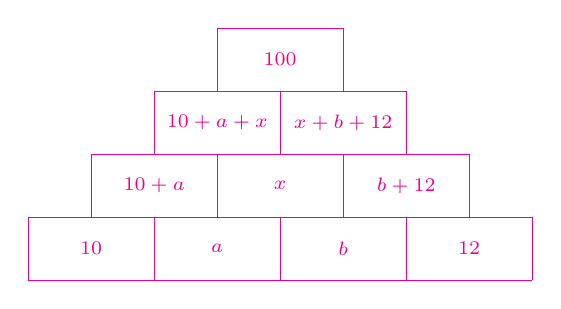
\begin{tikzpicture}[xscale=2, toancuabi,scale=0.8, node font=\scriptsize]
			\draw (0,0) grid (4,1);
			\draw (1,2) grid (3,3);
			\draw (0.5,1) rectangle (3.5,2);
			\draw (1.5,3) rectangle (2.5,4);
			\draw (1.5,1) --(1.5,2) (2.5,1) --(2.5,2);
			\draw (0.5,0.5) node {$10$};
			\draw (1.5,0.5) node {$a$};
			\draw (2.5,0.5) node {$b$};
			\draw (3.5,0.5) node {$12$};
			\draw (1,1.5) node {$10 + a $};
			\draw (2,1.5) node {$x$};
			\draw (3,1.5) node {$b+ 12$};
			\draw (1.5,2.5) node {$10 + a + x$};
			\draw (2.5,2.5) node {$x + b + 12$};
			\draw (2,3.5) node {$100$};
		\end{tikzpicture}
		\vspace*{-10pt}
	\end{figure}
	Vậy $100 = a + 10 + x + b + 12 + x = a + b + 2×x + 22$.
	\vskip 0.1cm
	Do $x = a + b$ nên $100 = 3\times x + 22$.
	\vskip 0.1cm
	Giải ra ta được $x = 26$.
	\vskip 0.1cm
	\textbf{\color{toancuabi}Bài $\pmb{10}$.} Mã PIN của bạn Kiên có dạng: $1ab3$, với $a$, $b$ là hai chữ số khác nhau và khác hai chữ số $1$, $3$.
	\vskip 0.1cm
	Ta thấy có $8$ cách chọn chữ số $a$ và $7$ cách chọn chữ số $b$.
	\vskip 0.1cm
	Do đó có $8\times 7 = 56$ cách chọn $2$ chữ số $a$ và $b$ hay có $56$ số khác nhau cho mã PIN của bạn Kiên.
\end{multicols}
%\newpage
%\graphicspath{{../toancuabi/pic/}}
%\begingroup
%\AddToShipoutPicture*{\put(106,650){
\includegraphics[scale=1]{../tieude.pdf}}}  
%\centering
%\endgroup
%\vspace*{55pt} 
%\begin{multicols}{2}
%	Thám tử Xuân Phong đôi khi phải đột nhập vào những nơi hoang vắng, kỳ bí để tìm ra được dấu tích của những kẻ gây án. Một lần nọ, sau bao ngày cải trang để bám sát, theo dõi manh mối, thám tử biết tên trùm tội phạm đang trốn tránh trong một ngôi nhà hẻo lánh ở ngoại ô. Vừa đến trước cửa của ngôi nhà gỗ cổ kính, Xuân Phong gặp một bà lão với đôi mắt tinh anh nhìn mình với vẻ bí mật ``thám tử đó phải không, tôi nhận ngay ra ngài, dù ngài đã cải trang rất kỹ. Phải chăng thám tử đang đi tìm tên trùm? Hắn đang ngồi dưới kia, trong căn phòng cùng những người trong Hiệp hội Thương Gia, nhưng vô cùng nguy hiểm nếu ngài dùng vũ lực ở đây để bắt hắn. Tôi mách ngài nhé, ở dưới đó, có $10$ người, trong đó có lão trùm và những kẻ đồng phạm của lão. Bọn họ là những kẻ luôn nói dối, nhưng cũng có thể có cả những người lương thiện, luôn nói thật, ở ngay bên cạnh. Ngài hãy dùng trí thông minh của mình, chỉ được hỏi rất hạn chế câu hỏi để phán đoán ra những kẻ phạm tội là ai. Ngài hỏi nhiều câu hơn sẽ nguy hiểm cho cả những thương gia lương thiện có thể có mặt ở đó. Và ngài hãy hứa với bà lão này sẽ đảm bảo an toàn cho tôi và gia đình, vì tôi đã liều mình thông báo tin mật này với thám tử".
%	\vskip 0.1cm
%	Theo lời bà lão mách bảo, Xuân Phong lần theo một chiếc cầu thang cũ nát và đi xuống một căn phòng khuất dưới tầng hầm. Vừa mở cửa ra, thám tử đã thấy có $10$ người ăn mặc chỉnh tề như nhau, ngồi nghiêm trang quanh một chiếc bàn mười cạnh, mỗi người ngồi tại đỉnh của hình mười cạnh. Ánh sáng lờ mờ trong phòng đủ chiếu rõ dòng chữ ``Cuộc họp thường niên Hiệp hội Thương gia -- Khu vực Duyên Hải". Thật khó để xác định ai là kẻ nói dối trong số họ, vì vẻ ngoài họ đều giống như những thương Gia thường gặp: quyền lực, sắc sảo và oai vệ.
%	\begin{figure}[H]
%		\centering
%		\vspace*{-5pt}
%		\captionsetup{labelformat= empty, justification=centering}
%		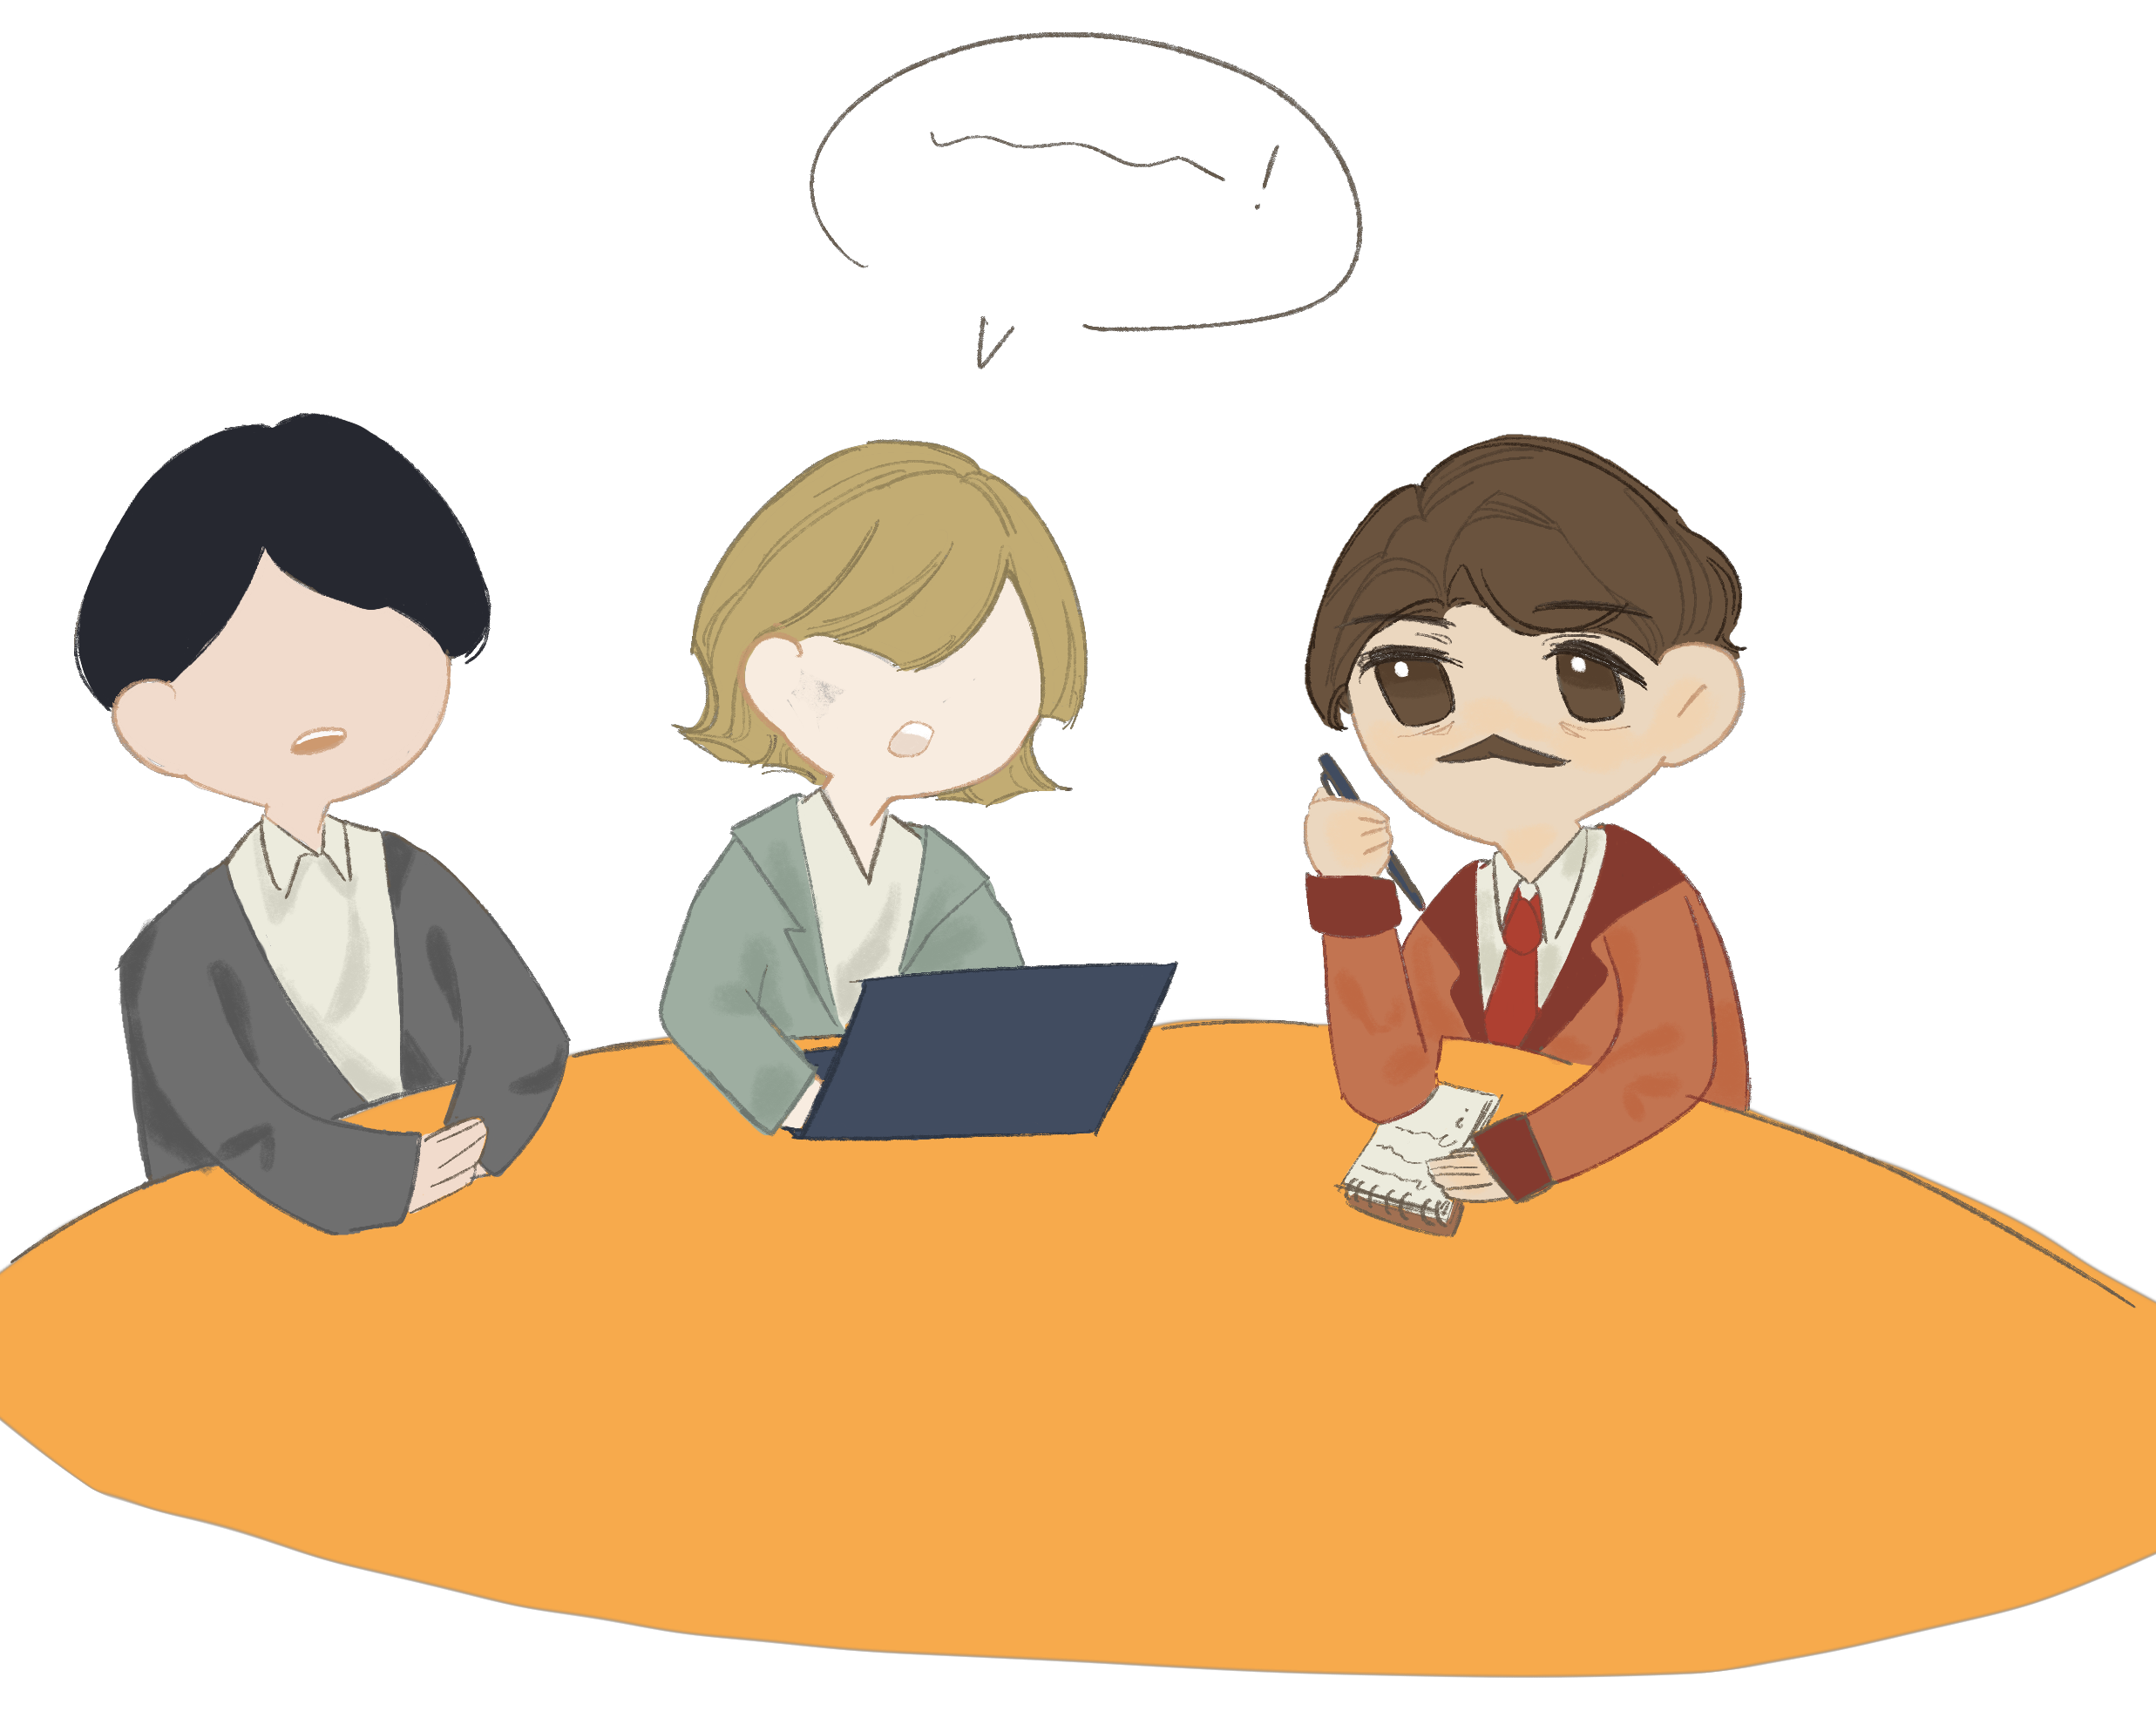
\includegraphics[width=1\linewidth]{xp}
%		\vspace*{-15pt}
%	\end{figure}
%	Theo quy định của Hiệp hội Thương gia dành cho những người ngoài, qua lời của bà lão, thám tử có thể đứng dậy bước tới một nơi bất kỳ nào đó trong căn phòng và chỉ được hỏi câu hỏi ``Khoảng cách từ chỗ tôi đứng đến người nói dối gần nhất trong số các anh là bao nhiêu?" cho tất cả những người trong phòng. Sau đó, mỗi người trong số $10$ người ngồi xung quanh bàn sẽ trả lời thám tử, lúc này đã cải trang thành một thương gia muốn gia nhập Hiệp hội. thám tử không được phép đứng lên mặt bàn và tất cả mọi người, kể cả thám tử, đều được phép dùng thước để đo khoảng cách tuỳ ý. Ta cũng được biết rằng ngoài $10$ người và thám tử, trong phòng không còn có người lạ nào khác, hơn nữa $10$ người đều biết rõ ai trong số họ là nói thật và ai trong số họ là nói dối. Em hãy cho biết Xuân Phong có thể sử dụng ít nhất bao nhiêu câu hỏi như trên để biết chắc chắn ai trong số những người ngồi quanh bàn là nói~dối?
%\end{multicols}
%\newpage
%\begingroup
%\AddToShipoutPicture*{\put(115,670){
\includegraphics[scale=1]{../tieude11.pdf}}} 
%\centering
%\endgroup
%\vspace*{35pt}
%
%\begin{multicols}{2}
%	$\pmb{1.}$ Tuấn và Tú cùng tham gia một giải thi đấu cờ vua cùng các bạn học sinh khác trong trường. Hai bạn tổng cộng ghi được $6{.}5$ điểm, trong khi tất cả các bạn học sinh còn lại đều ghi được số điểm bằng nhau. Hỏi có tất cả bao nhiêu học sinh tham gia giải cờ vua đó? (Biết rằng trong giải thi đấu, mỗi người tham gia thi đấu đúng một ván với mỗi người còn lại, ghi được $1$ điểm sau mỗi trận thắng, $0{.}5$ điểm sau mỗi trận hoà và $0$ điểm sau mỗi trận thua).
%	\begin{figure}[H]
%		\centering
%		\vspace*{-5pt}
%		\captionsetup{labelformat= empty, justification=centering}
%		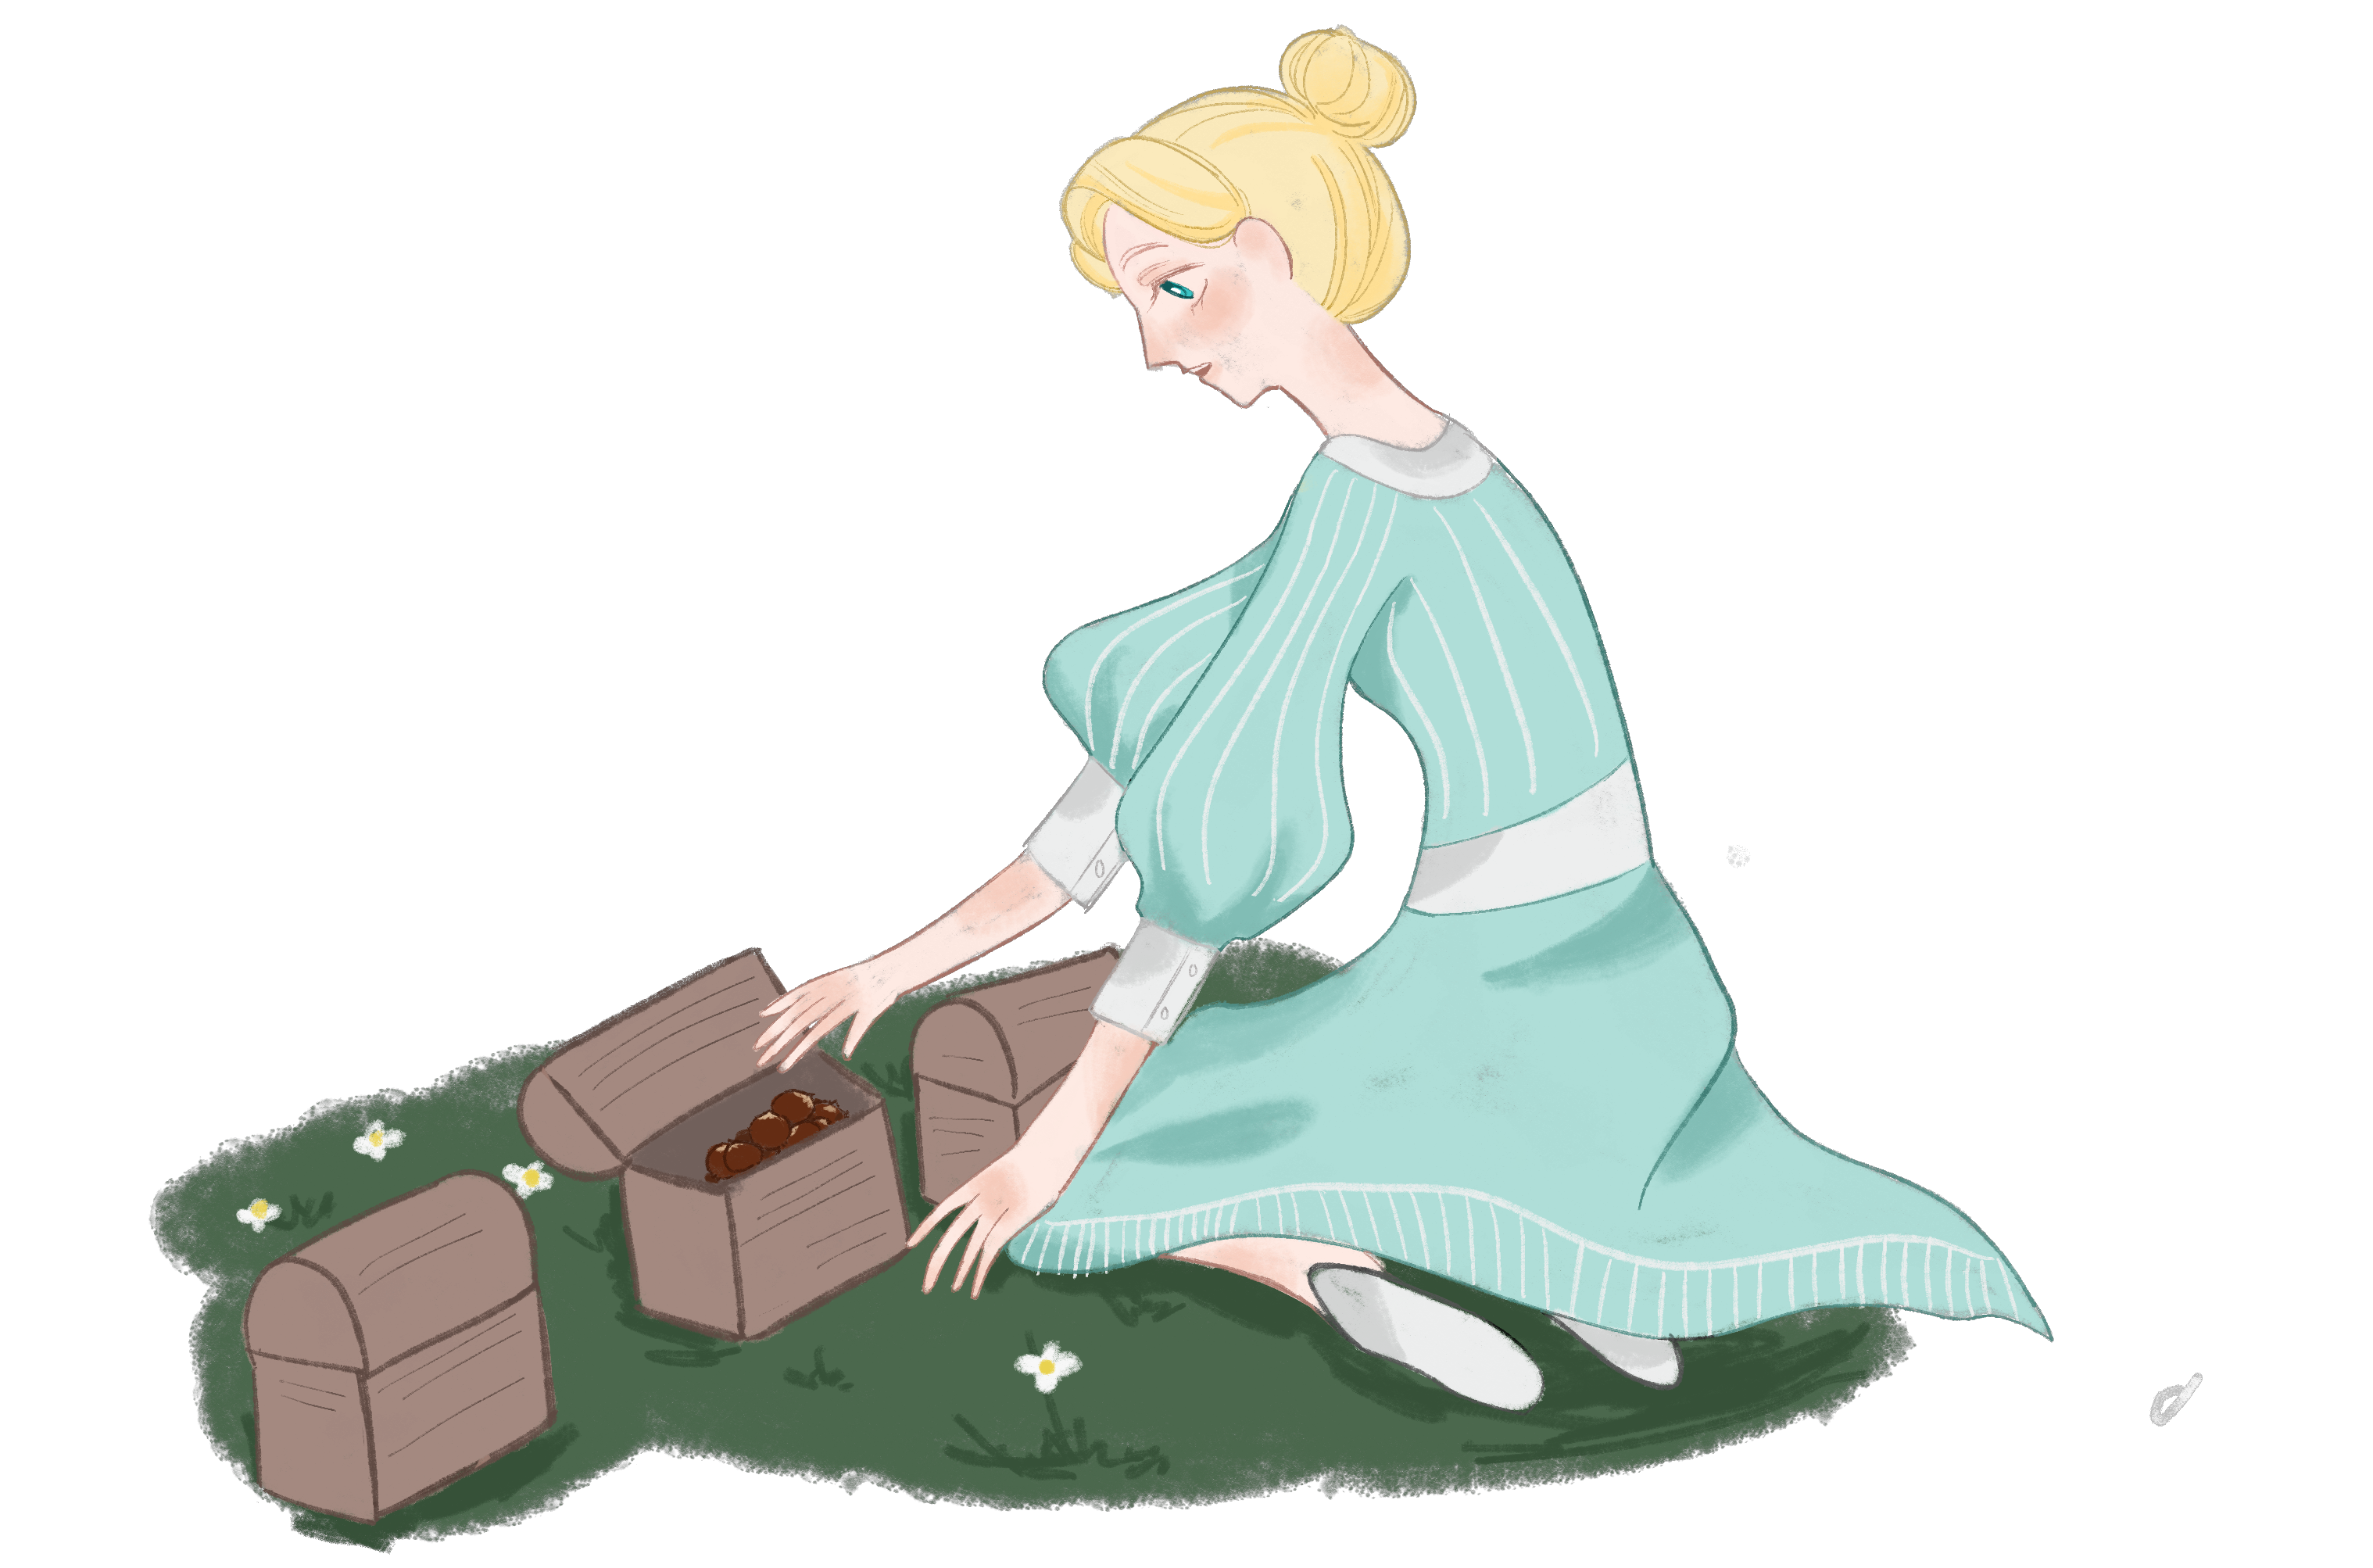
\includegraphics[width=1\linewidth]{Hinh1}
%		\vspace*{-20pt}
%	\end{figure}
%	$\pmb{2.}$ 	Lớp $6$A gồm $22$ bạn chia thành hai đội: Xanh gồm các bạn nam và Đỏ gồm các bạn nữ để tổ chức thi tài đối đáp, trả lời thông minh. Đầu tiên, bạn Hoa ở nhóm Đỏ đối đáp với $6$ bạn nam ở nhóm Xanh và giành chiến thắng. Tiếp theo, bạn Mai ở nhóm Đỏ đối đáp với $7$ bạn nam ở nhóm Xanh và cũng giành chiến thắng. Tiếp tục bạn Huệ ở nhóm Đỏ cũng chiến thắng $8$ bạn nam ở nhóm Xanh. Cứ tiếp tục như vậy, cuối cùng bạn Hà ở nhóm Đỏ đã đối đáp thông minh với toàn bộ các bạn nam ở nhóm Xanh và giành chiến thắng chung cuộc. Hỏi trong lớp có tất cả bao nhiêu bạn nam?
%	\begin{figure}[H]
%		\centering
%		\vspace*{-5pt}
%		\captionsetup{labelformat= empty, justification=centering}
%		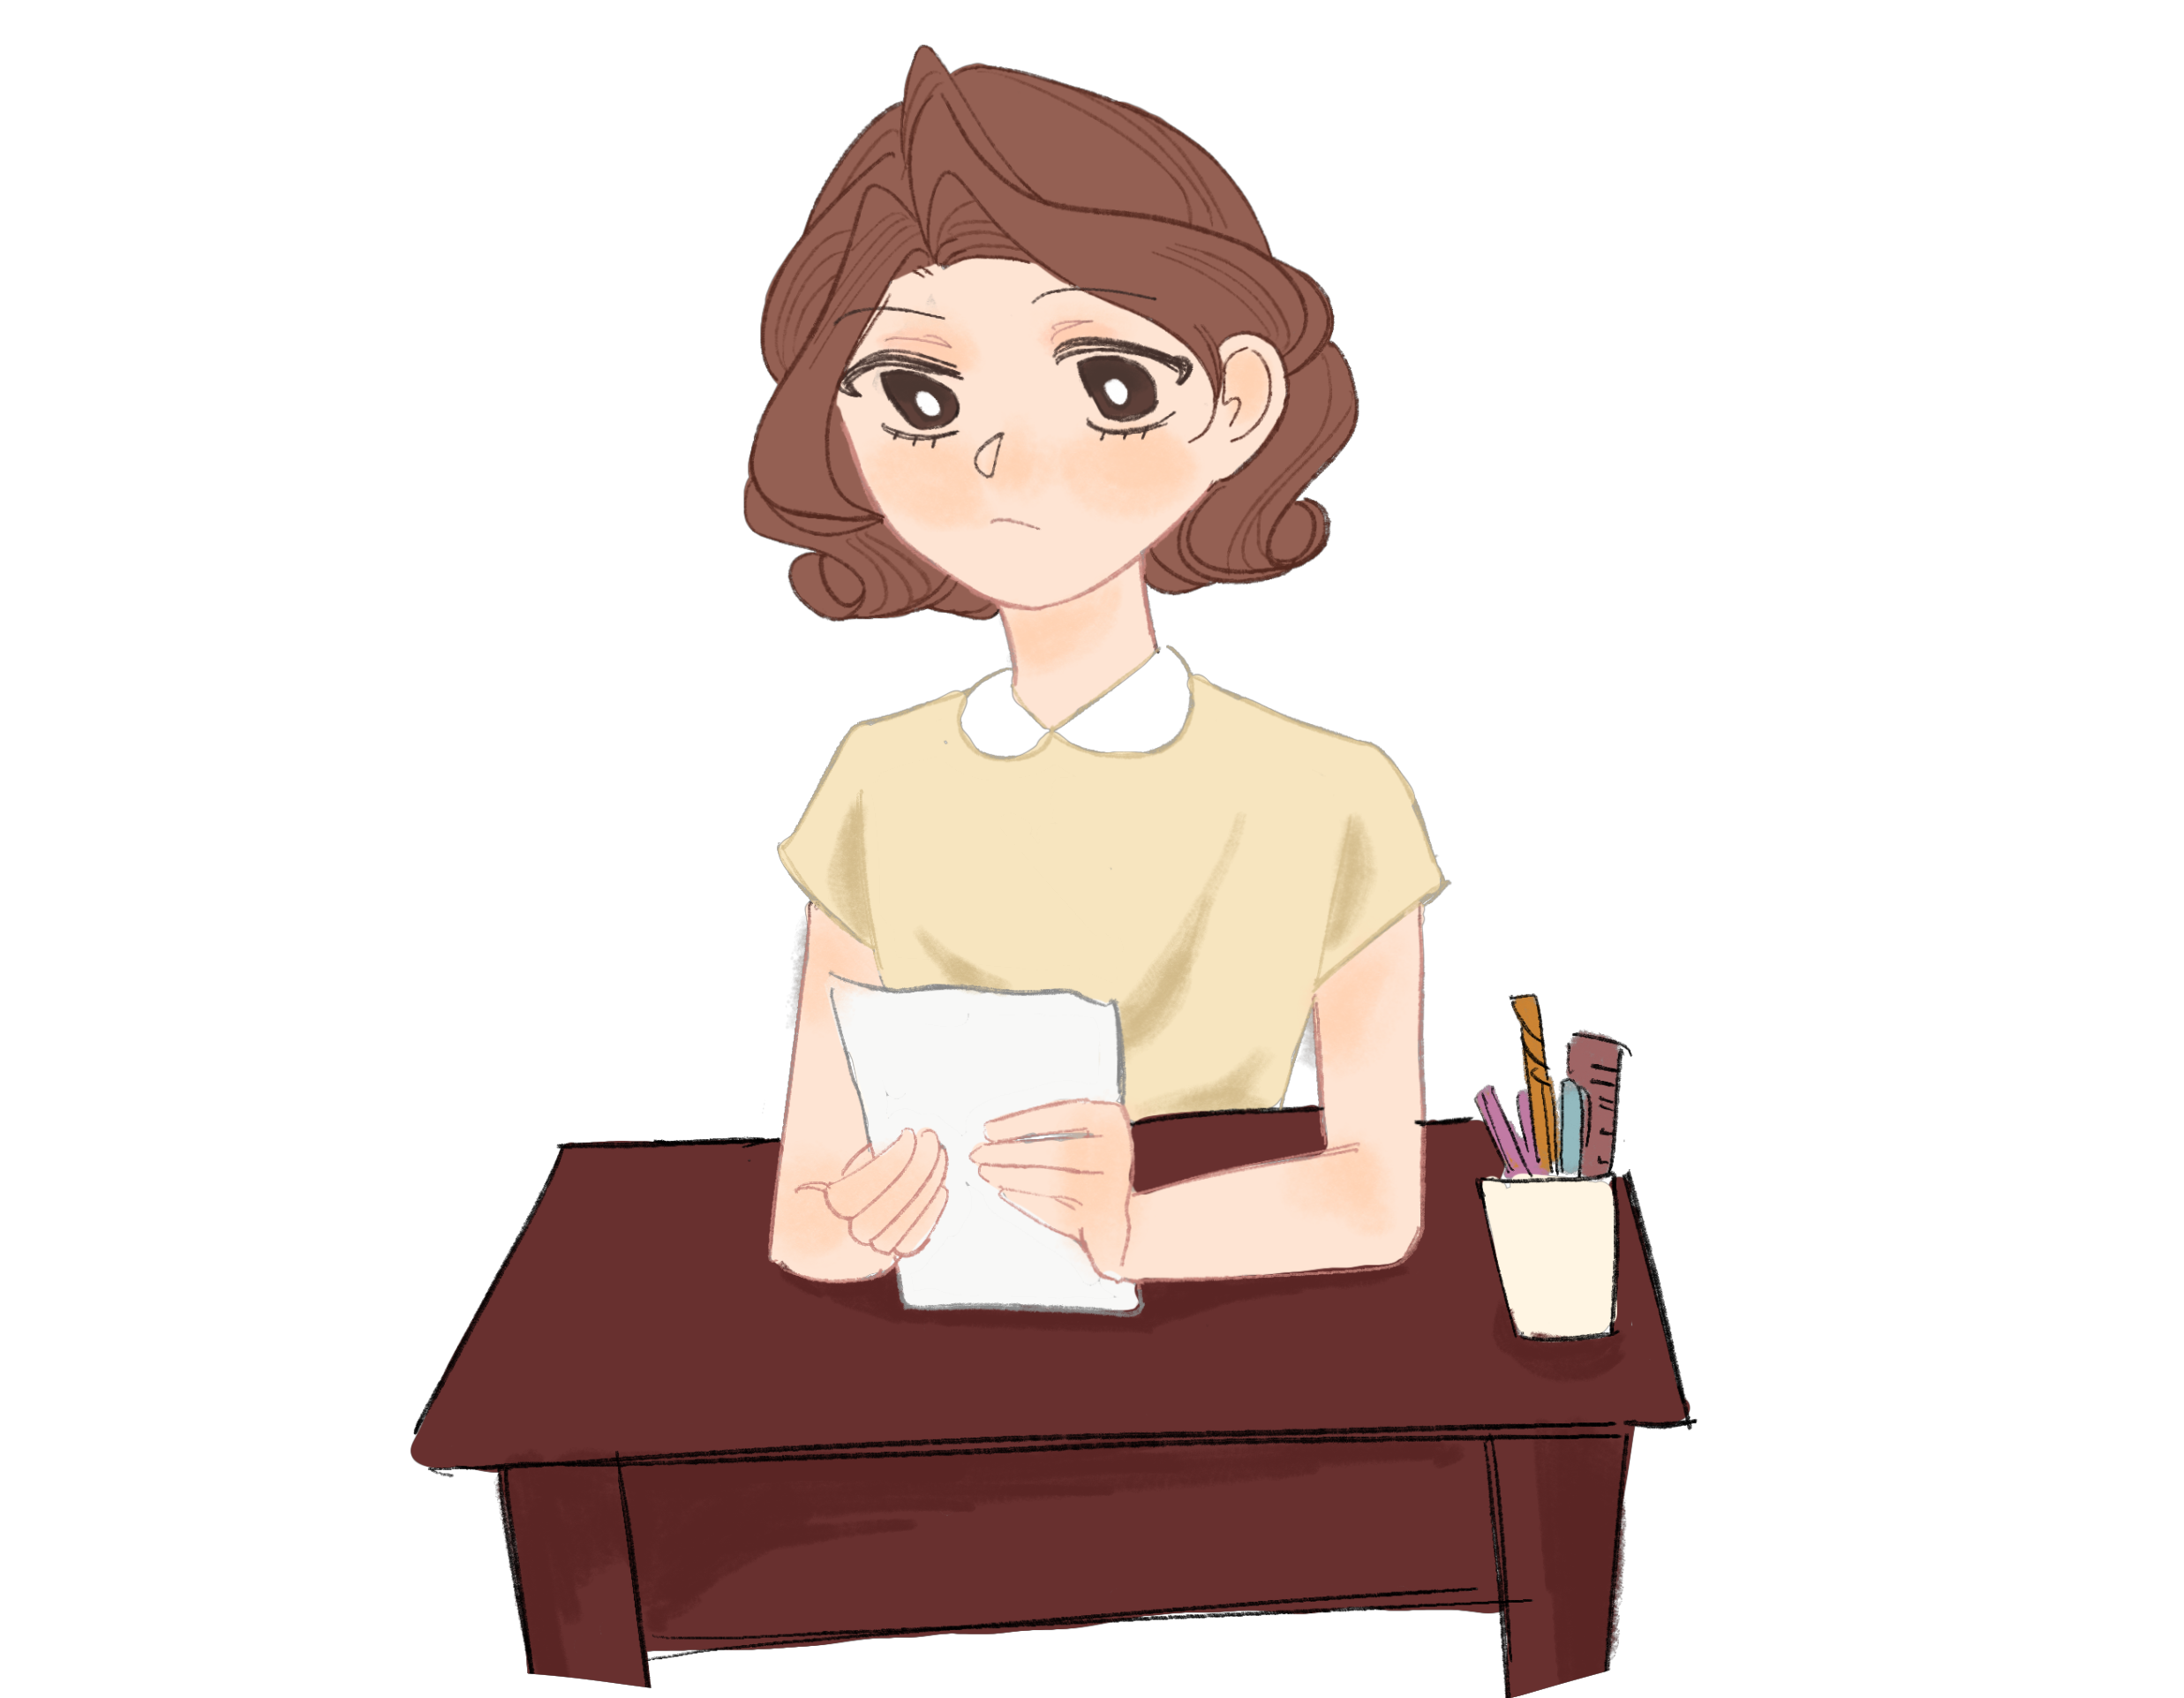
\includegraphics[width=1.01\linewidth]{Hinh2}
%		\vspace*{-5pt}
%	\end{figure}
%	$\pmb{3.}$ 	Có bốn chủ doanh nghiệp tới thăm trường học cũ của mình, mang theo một số món quà với dự định sẽ trao tặng cho các học sinh đang học ở đó. Khi tất cả $252$ em học sinh được mời xếp thành một hàng ngang, chủ doanh nghiệp thứ nhất tặng quà cho mỗi em đứng thứ tư trong hàng (các em ở số thứ tự $4,8,12,$ \ldots). Chủ doanh nghiệp thứ hai lại tặng quà cho mỗi em đứng thứ bảy (các em ở số thứ tự $7,14,21$, \ldots). Chủ doanh nghiệp thứ ba trao tặng quà cho mỗi em đứng thứ mười một (các em ở số thứ tự $11,22,33$, \ldots). Chủ doanh nghiệp thứ tư sẽ tặng quà cho các em còn lại. Hỏi có bao nhiêu em học sinh nhận được quà từ mỗi chủ doanh nghiệp?
%	\begin{figure}[H]
%		\centering
%		\vspace*{-5pt}
%		\captionsetup{labelformat= empty, justification=centering}
%		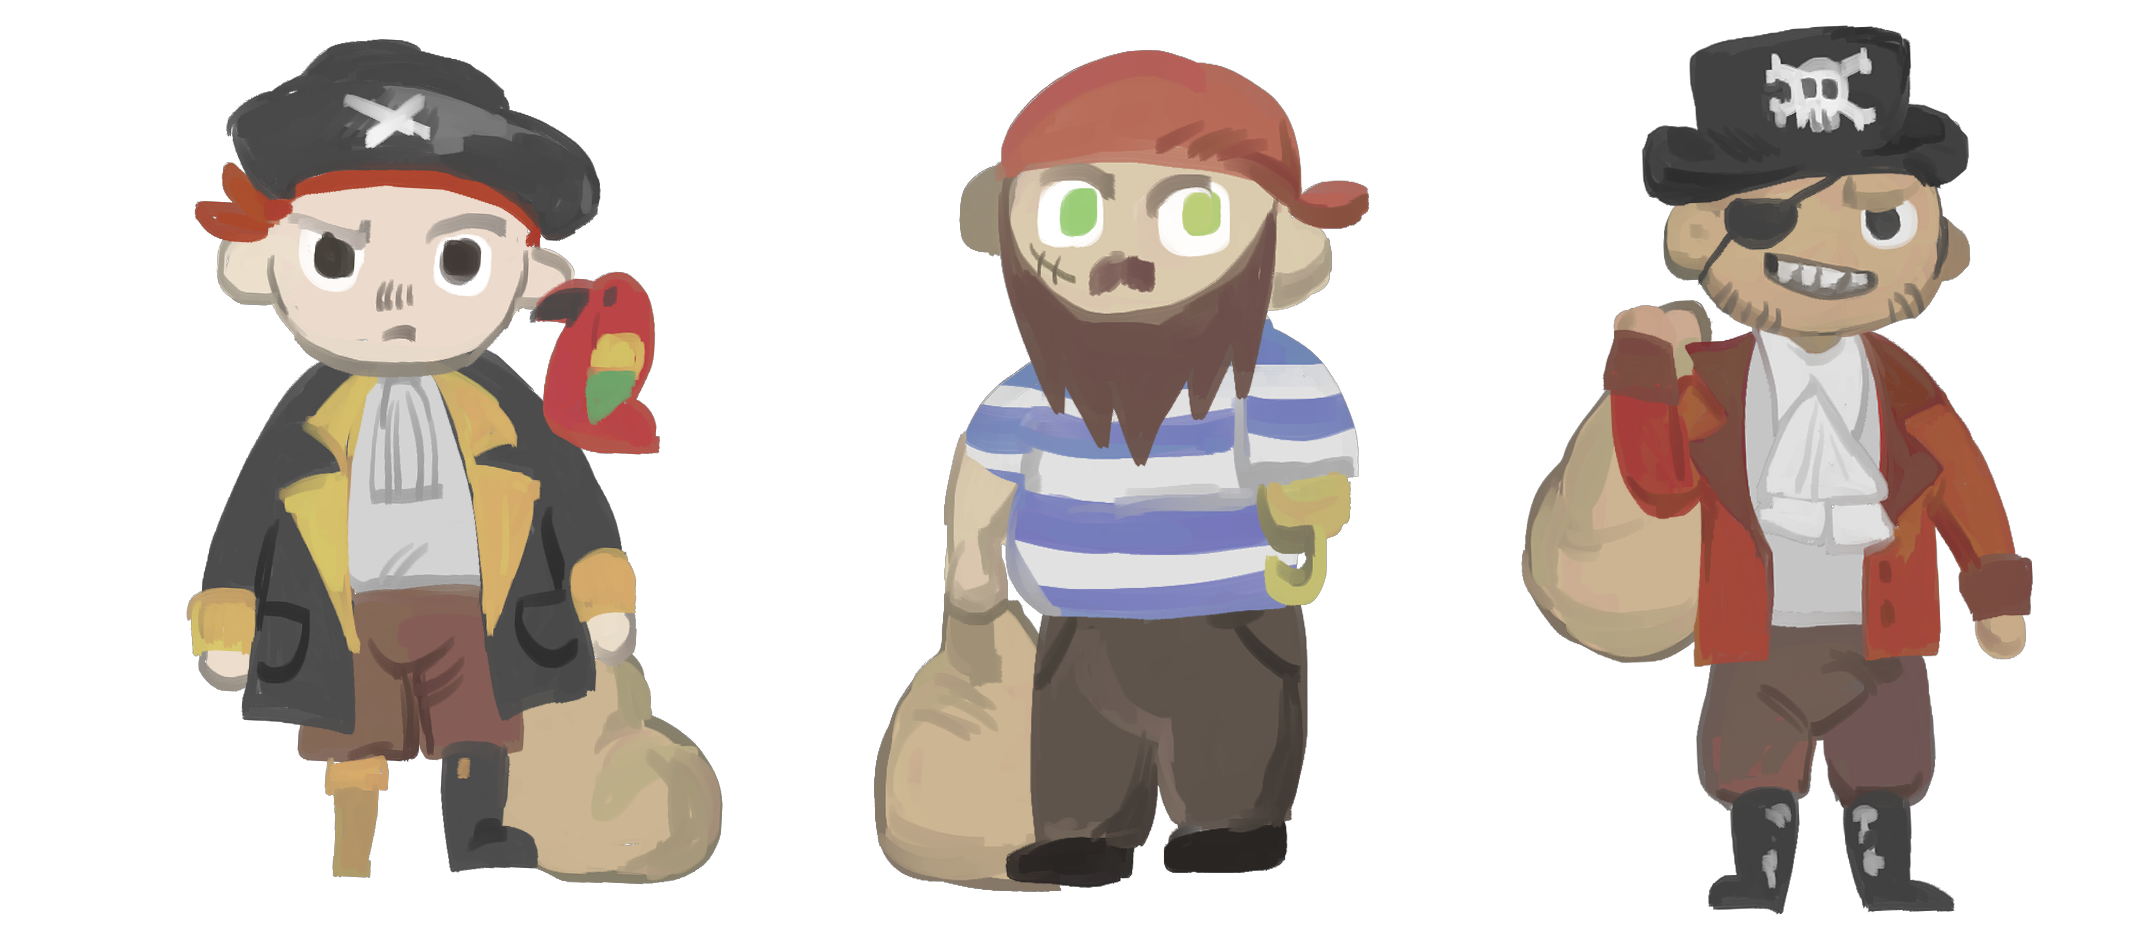
\includegraphics[width=1\linewidth]{Hinh3}
%		\vspace*{-15pt}
%	\end{figure}
%	$\pmb{4.}$ 	Có ba nhà tài trợ quyết định giúp đỡ một tạp chí khoa học thường thức với tên gọi là Phi. Nhà tài trợ Quốc trao tặng một khoản tiền tính bằng dollar gồm có $4$ chữ số: $2$ chữ số đứng trước dấu phẩy, và hai chữ số sau dấu phẩy, trong đó số cent lẻ (tức là hai chữ số đứng sau dấu phẩy) bằng với đúng số dollar chẵn (tức là hai chữ số đứng trước dấu phẩy; ta nhớ lại $100$ cent $= 1$ dollar). Nhà tài trợ Minh tặng số tiền với số dollar chẵn lớn hơn $3$ dollar so với số dollar chẵn mà nhà tài trợ Quốc đã tặng nhưng số cent lẻ lại ít hơn $8$ lần số cent lẻ của nhà tài trợ Quốc. Nhà tài trợ Vũ hào phóng đem tặng số tiền bằng $1/7$ tổng số tiền của hai nhà tài trợ Quốc và Minh đã trao cộng lại. Hỏi số tiền ủng hộ của ba nhà tài trợ cho tạp chí Phi là bao nhiêu?
%	\begin{figure}[H]
%		\centering
%%		\vspace*{-5pt}
%		\captionsetup{labelformat= empty, justification=centering}
%		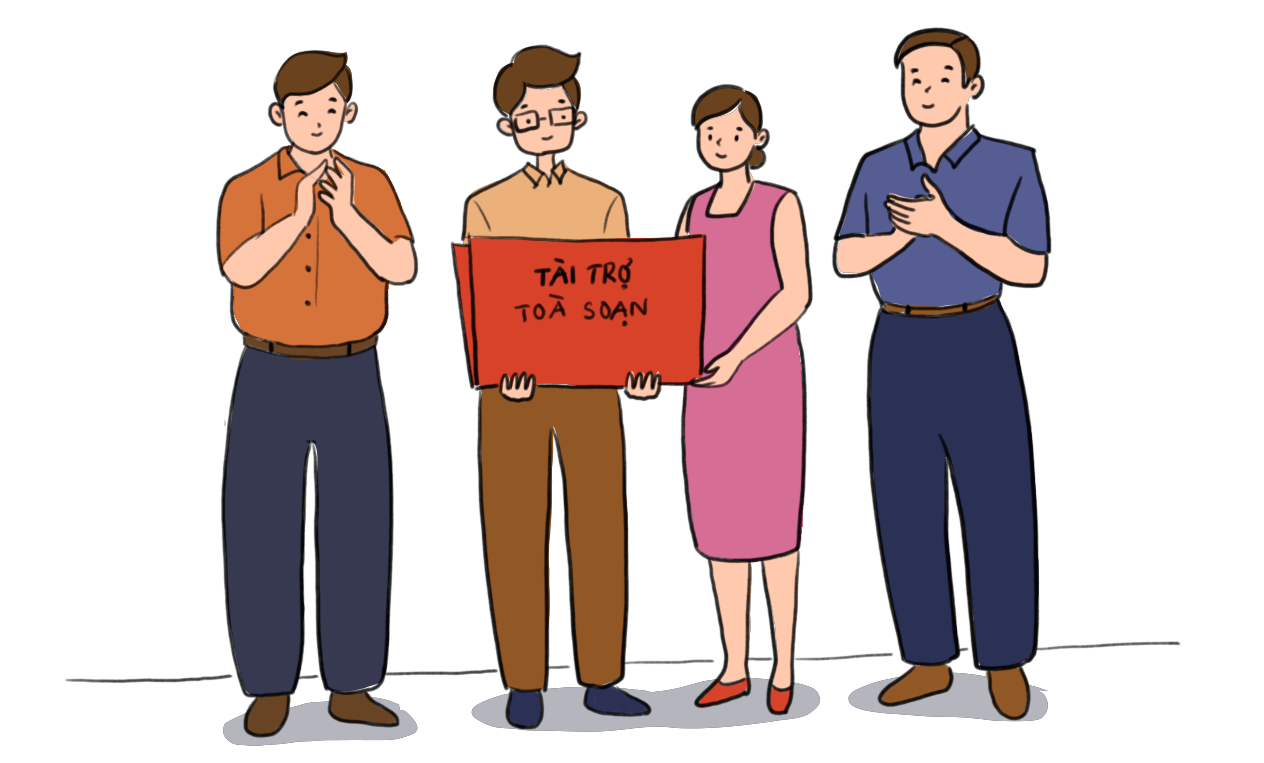
\includegraphics[width=0.8\linewidth]{Hinh4}
%		\vspace*{-10pt}
%	\end{figure}
%	\vskip 0.1cm
%	$\pmb{5.}$ 	Trên hòn đảo Ngọc ở giữa một đại dương xanh ngắt có $100$ thổ dân sinh sống, một số người trong họ luôn nói dối, còn những người còn lại luôn nói thật. Mỗi một thổ dân thờ phụng đúng một trong ba vị thần: thần Mặt trời, thần Mặt trăng hoặc thần Đất. Người ta hỏi mỗi thổ dân ba câu hỏi sau đây:
%	\begin{figure}[H]
%		\centering
%		\vspace*{-5pt}
%		\captionsetup{labelformat= empty, justification=centering}
%		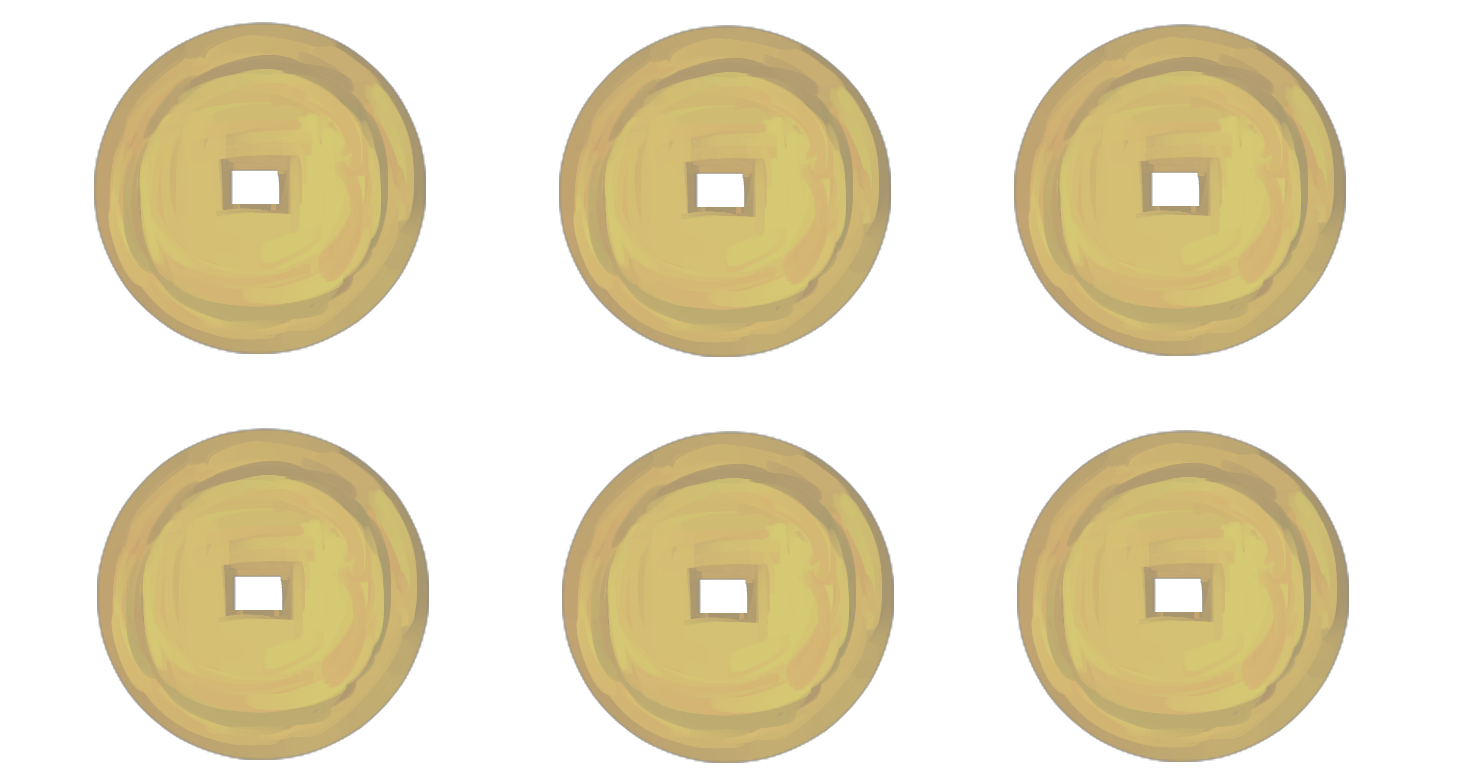
\includegraphics[width=1\linewidth]{Hinh5}
%		\vspace*{-20pt}
%	\end{figure}
%	$1.$ Ông (bà) có thờ phụng thần Mặt trời hay không?
%	\vskip 0.1cm
%	$2.$ Ông (bà) có thờ phụng thần Mặt trăng hay không?
%	\vskip 0.1cm
%	$3.$ Ông (bà) có thờ phụng thần Đất hay không?
%	\vskip 0.1cm
%	Có $60$ người trả lời khẳng định ``có" với câu hỏi thứ nhất, $40$ người trả lời khẳng định ``có" với câu hỏi thứ hai và $30$ người trả lời khẳng định ``có" với câu hỏi thứ ba. Hỏi trên đảo Ngọc có bao nhiêu thổ dân nói dối?
%	\vskip 0.1cm
%	$\pmb{6.}$ 	Có $100$ em học sinh được mời tới buổi tổng kết cuối năm học của nhà trường. Các ghế trong phòng họp được xếp ngay ngắn thẳng hàng theo dạng một hình vuông với $10$ dãy ghế, mỗi dãy có đúng $10$ chiếc ghế. Buổi họp phải diễn ra muộn hơn do bị cắt điện, vì thế các em học sinh bắt đầu bàn luận trao đổi với các bạn bên cạnh về kết quả điểm trung bình của mình. Em học sinh nào thấy trong tất cả những bạn ngồi kề sát mình: bên trái, bên phải, đằng sau, đằng trước và theo các đường chéo, chỉ có tối đa một bạn có điểm trung bình cao hơn hoặc bằng điểm trung bình của  mình, sẽ tự coi mình là ``có thành tích".
%	\begin{figure}[H]
%		\centering
%		\vspace*{-10pt}
%		\captionsetup{labelformat= empty, justification=centering}
%		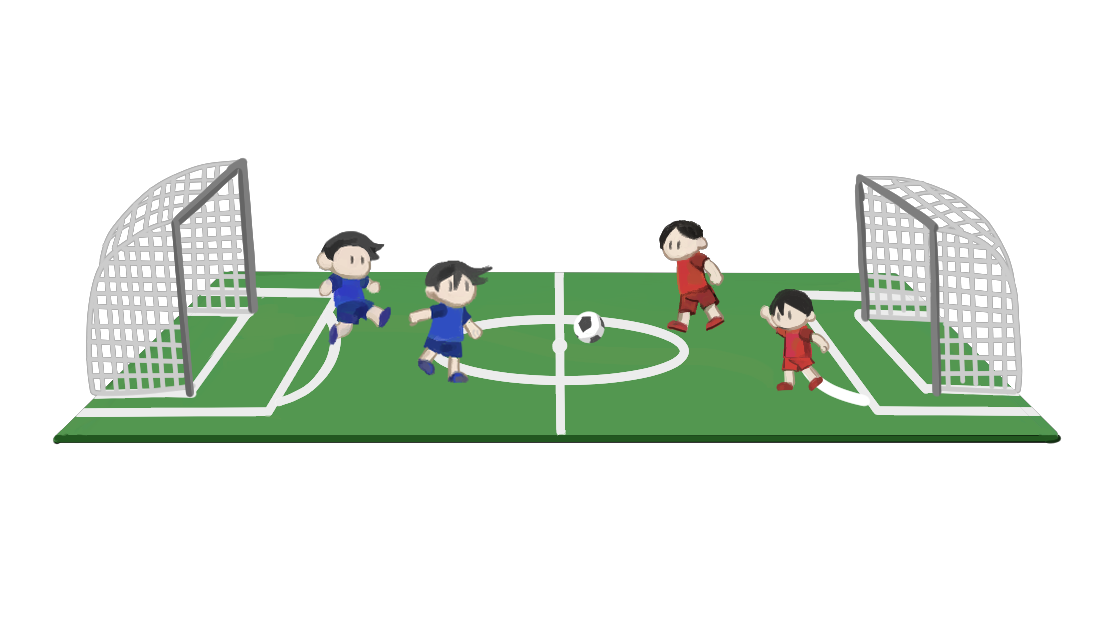
\includegraphics[width=0.85\linewidth]{Hinh6}
%		\vspace*{-10pt}
%	\end{figure}
%	Hỏi trong buổi họp đó có thể có tối đa bao nhiêu em học sinh đã tự coi mình là ``có thành tích" trong học tập?
%\end{multicols}
%\vspace*{-10pt}
%{\color{toancuabi}\rule{1\linewidth}{0.1pt}}
%\begingroup
%\AddToShipoutPicture*{\put(114,178){
\includegraphics[scale=1]{../tieude2.pdf}}} 
%\centering
%\endgroup
%\vspace*{75pt}
%
%\begin{multicols}{2}
%	$\pmb{1.}$ Các bạn nam mang kẹo tới lớp để tặng cho các bạn nữ. Bạn Phúc nói rằng mình đã mang tới đúng một nửa tổng số kẹo. Bạn Kiên nói rằng mình đã mang tới đúng một phần ba tổng số kẹo và chỉ chia kẹo của mình cho Mai và Tuyết, hơn nữa Mai được nhiều hơn so với Tuyết là $3$ chiếc kẹo. Em hãy chứng tỏ rằng có một bạn trong số Phúc và Kiên đã \linebreak nhầm lẫn.\\
%	\textit{Lời giải.} Giả sử cả hai bạn Phúc và Kiên đều không nhầm lẫn. Do Phúc không nhầm, nên tổng số kẹo được mang tới lớp phải là số chẵn (gấp $2$ lần số kẹo mà Phúc mang tới). Do Kiên cũng mang tới một số kẹo là số nguyên, bằng $1/3$ của một số chẵn, nên Kiên cũng mang tới một số kẹo là số chẵn. Theo lời của Kiên, số kẹo mà cậu đã tặng cho các bạn nữ là một số lẻ, do số kẹo mà Mai và Tuyết nhận được khác tính chẵn lẻ (hơn kém nhau là $3$ chiếc, mà $3$ là một số lẻ), mà tổng của hai số khác tính chẵn lẻ là một số lẻ. Ta nhận được mâu thuẫn. Suy ra có ít nhất một bạn nam trong số Phúc và Kiên đã nhầm lẫn.
%	\begin{figure}[H]
%			\centering
%		\vspace*{-5pt}
%		\captionsetup{labelformat= empty, justification=centering}
%		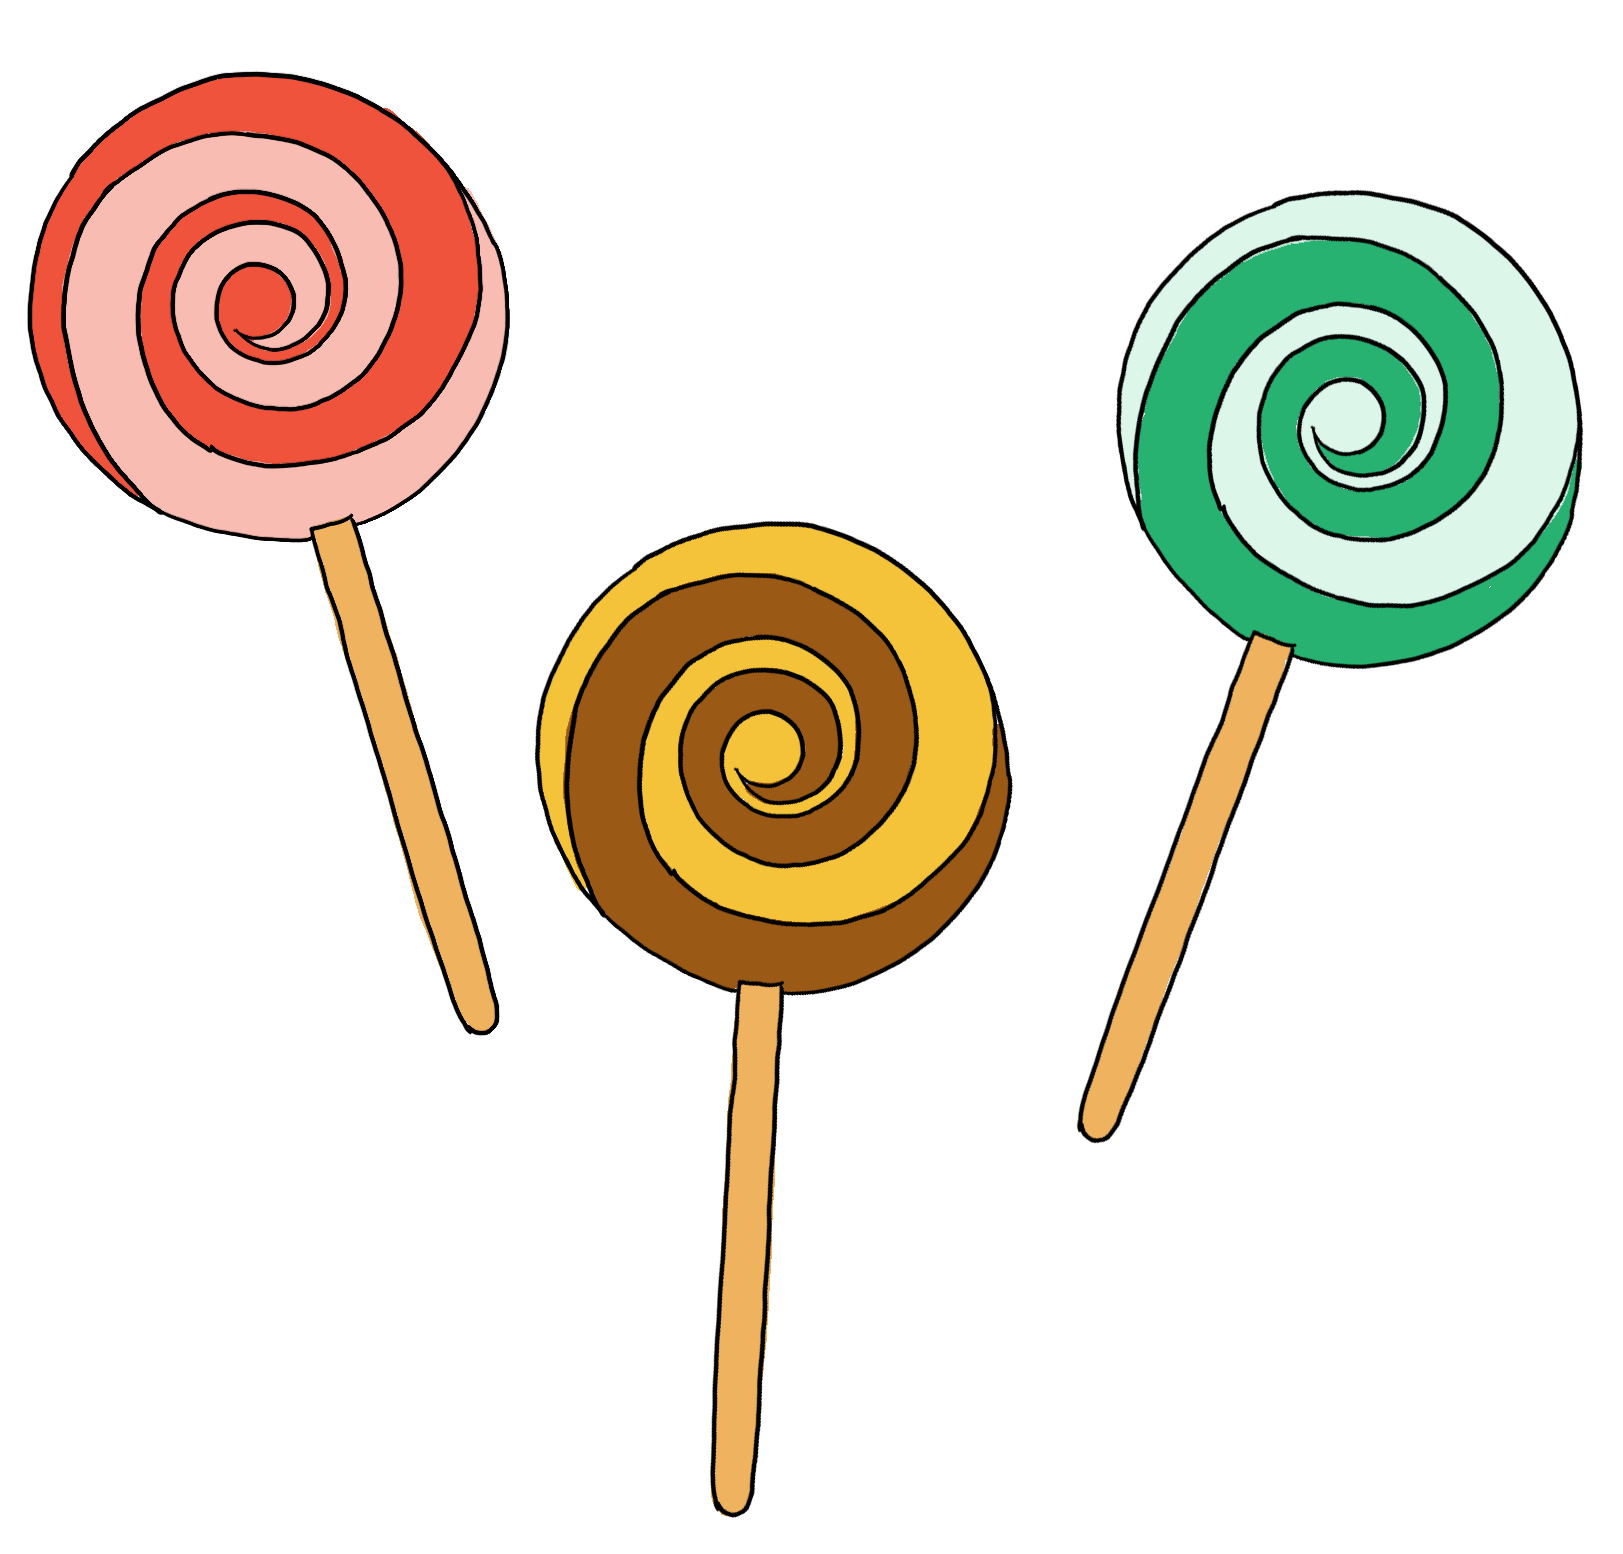
\includegraphics[width=0.6\linewidth]{Pi7_bai1}
%		\vspace*{-10pt}
%	\end{figure}
%	$\pmb{2.}$ Ba người thợ cùng đào một chiếc hố. Họ luân phiên lần lượt làm việc, mỗi người làm việc trong một thời gian nhất định. Nếu trong khi một người làm việc hai người còn lại cũng đồng thời đào hố thì hai người này sẽ đào được đúng một nửa hố. Hỏi nếu cả ba người cùng đồng thời đào thì họ sẽ làm nhanh hơn được bao nhiêu lần so với cách làm luân phiên ban đầu?
%	\begin{figure}[H]
%		\centering
%		\vspace*{-5pt}
%		\captionsetup{labelformat= empty, justification=centering}
%		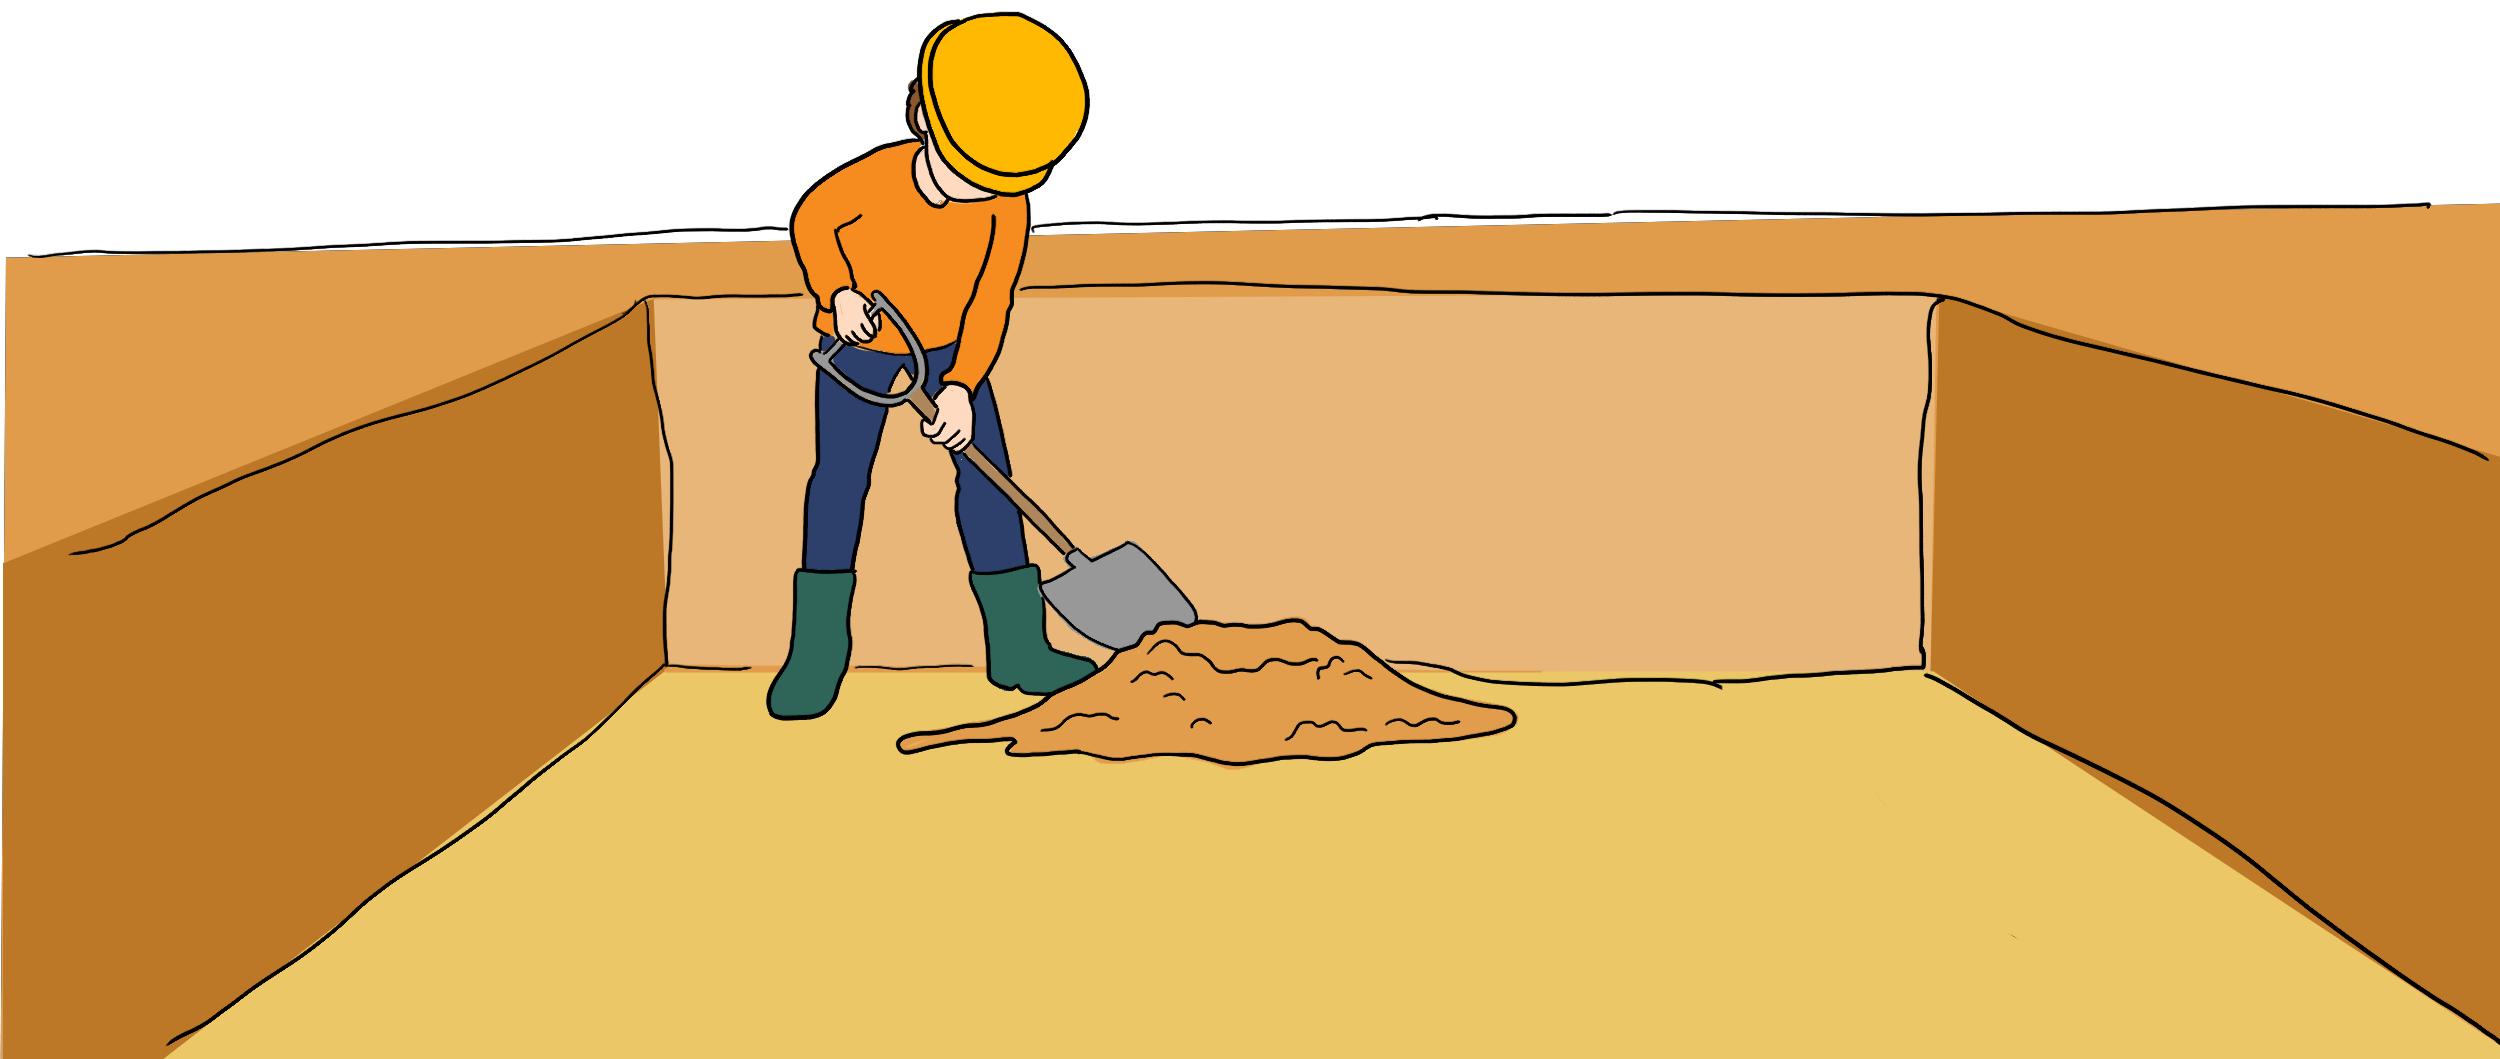
\includegraphics[width=1\linewidth]{Pi7_bai2}
%		\vspace*{-20pt}
%	\end{figure}
%	\textit{Lời giải.} 	Giả sử trong thời gian mỗi người đào ở chiếc hố ban đầu, hai người còn lại sẽ đi đào một chiếc hố bổ sung thêm khác. Như vậy khi kết thúc công việc, cùng với chiếc hố ban đầu, họ sẽ đào thêm được $3\cdot 0{.}5 = 1{.}5$ chiếc hố. Do đó, nếu cả ba người cùng làm công việc đào, thì trong cùng số thời gian như ban đầu, họ sẽ đào được $1+1{.}5=2{.}5$ (hố). Vậy, nếu cả ba người cùng đào thì họ sẽ làm nhanh hơn được $2{.}5$ lần so với cách đào luân phiên lần lượt như ban đầu.
%	\vskip 0.1cm
%	$\pmb{3.}$ Ba bạn Gấu, Thỏ và Mèo cùng quyết định xây một con đường từ nhà tới bờ suối với chiều dài $160m$. Các bạn thoả thuận sẽ đầu tư cho dự án mở đường quan trọng này với công sức đều như nhau. Cuối cùng khi dự án hoàn thành, hoá ra bạn Thỏ đã xây được $60$ mét đường, bạn Mèo xây được $100$ mét đường, còn bạn Gấu mải ngủ đông nên không xây được mét nào. Tuy nhiên, Gấu mang tới đóng góp bằng tiền cho dự án là $16$ triệu đồng từ số mật ong bán được của mình. Hỏi hai bạn Mèo và bạn Thỏ cần phải phân chia số tiền cho nhau như thế nào?
%	\begin{figure}[H]
%		\centering
%		\vspace*{-5pt}
%		\captionsetup{labelformat= empty, justification=centering}
%		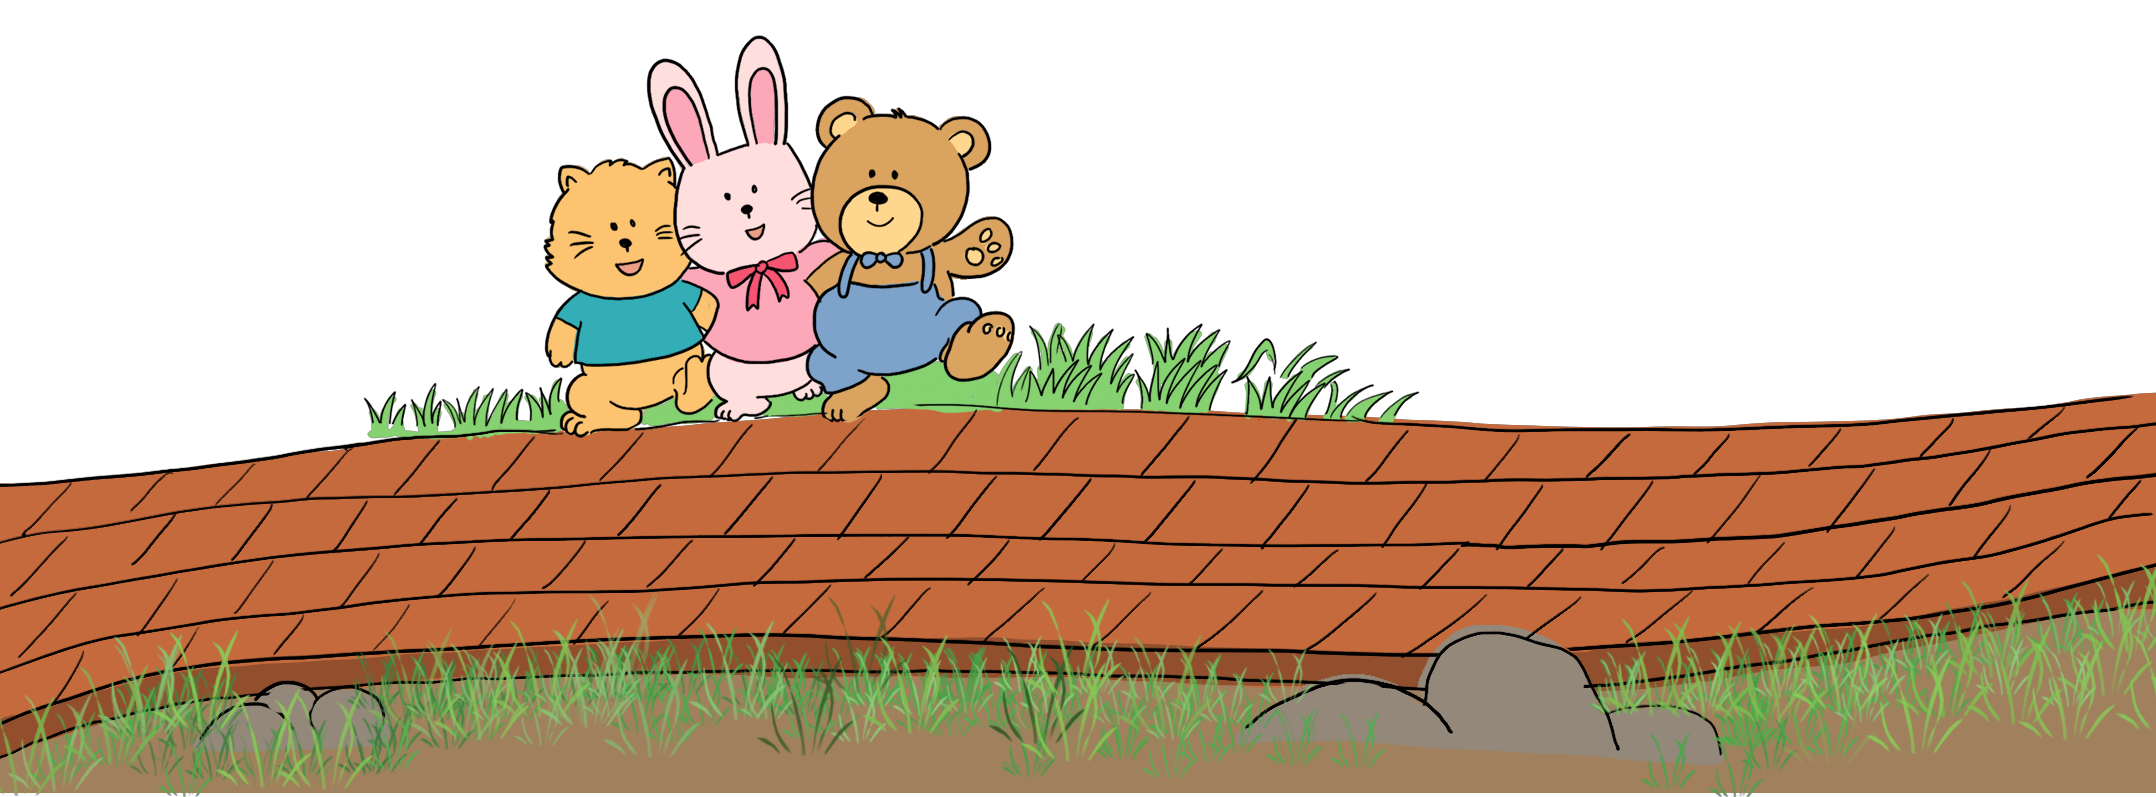
\includegraphics[width=1\linewidth]{Pi7_bai3}
%		\vspace*{-15pt}
%	\end{figure}
%	\textit{Lời giải.} 	Mỗi bạn theo kế hoạch phải xây đúng $\dfrac{160}{3} = 53\dfrac{1}{3}$  mét đường. Thỏ xây được $60$ (m) và Gấu xây được $100$ (m). Như vậy bạn Thỏ đã xây thay cho bạn Gấu số mét đường là
%	\begin{align*}
%		60 - 53 \frac{1}{3} = 6 \frac{2}{3}= \frac{20}{3} \text{ (m)},
%	\end{align*}
%	còn bạn Mèo đã xây thay cho bạn Gấu số mét đường
%	\begin{align*}
%		100- 53 \frac{1}{3} = 46 \frac{2}{3}=\frac{140}{3} \text{ (m).}
%	\end{align*}
%	Vì vậy số tiền mà bạn Gấu mang tới phải chia cho Thỏ và Mèo theo tỷ lệ $2: 14$, tức là Mèo được $14$ triệu đồng, còn Thỏ được $2$ triệu đồng từ số tiền đóng góp công sức của Gấu.
%	\vskip 0.1cm
%	$\pmb{4.}$ Bé Ly phải đi trồng hoa vào một hàng các chậu rất dài đặt thành hàng dọc ở công viên. Bé được giao nhiệm vụ là phải trồng hai loại hoa khác nhau vào hai chiếc chậu nếu giữa hai chậu này có đúng hai chiếc chậu, hoặc đúng ba chiếc chậu, hoặc đúng năm chiếc chậu khác. Hỏi bé Ly phải cần ít nhất bao nhiêu loại hoa để thực hiện được nhiệm vụ?
%	\begin{figure}[H]
%		\centering
%		\vspace*{-5pt}
%		\captionsetup{labelformat= empty, justification=centering}
%		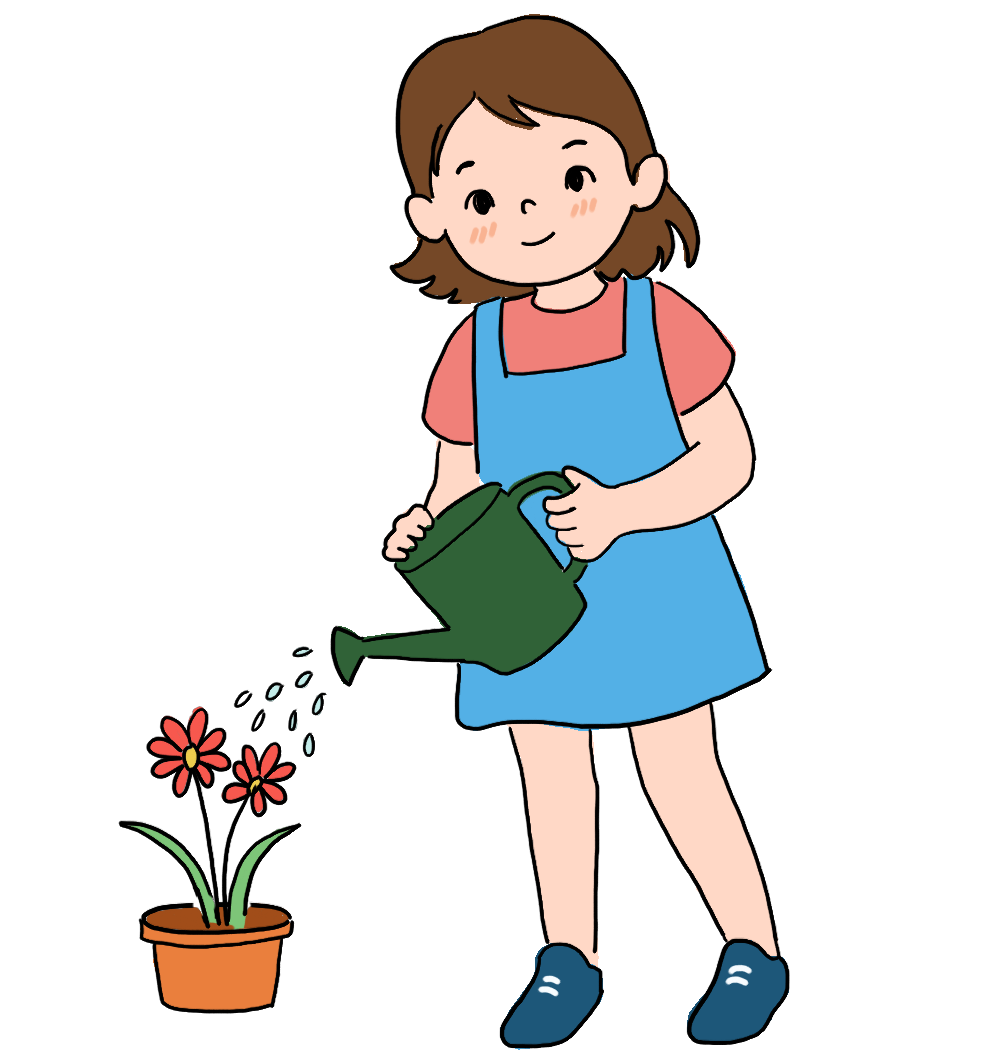
\includegraphics[width=0.45\linewidth]{Pi7_bai4}
%		\vspace*{-10pt}
%	\end{figure}
%	\textit{Lời giải.} Trước tiên ta thấy rằng bé Ly có thể chỉ cần $3$ loại hoa là thực hiện được nhiệm vụ. Thật vậy, giả sử Ly có $3$ loại là $A, B, C$. Khi đó nếu Ly trồng $3$ chậu đầu tiên trong hàng bằng loại $A$, $3$ chậu tiếp theo bằng loại $B$, $3$ chậu tiếp loại $C$ và lại $3$ chậu tiếp theo quay lại bằng loại $A$, vv \ldots thì rõ ràng yêu cầu đặt ra được thực hiện. 
%	\vskip 0.1cm
%	Bây giờ giả sử Ly chỉ có $2$ loại hoa là $A$ và $B$. Nếu Ly trồng ở chậu thứ nhất bằng hoa loại $A$ (không mất tính tổng quát), suy ra các chậu có số thứ tự tiếp theo là $4, 5, 7$ phải được trồng bằng hoa loại $B$. Nhưng khi đó giữa hai chậu số $4$ và số $7$ đều được trồng cùng loại hoa $B$ nhưng giữa chúng có đúng hai chậu khác là số $5$ và số $6$, suy ra mâu thuẫn với yêu cầu.
%	\vskip 0.1cm
%	Vậy Ly cần ít nhất $3$ loại hoa để trồng theo yêu cầu đặt ra.
%	 \vskip 0.1cm
%	$\pmb{5.}$ Trước một trận bóng đá giữa hai đội Xóm Đông và Xóm Bắc có $5$ dự đoán kết quả được đưa ra:
%	\vskip 0.1cm
%	$a)$	Sẽ không có tỷ số hoà;
%	\vskip 0.1cm
%	$b)$	Đội Xóm Đông sẽ bị thủng lưới;
%	\vskip 0.1cm
%	$c)$	Đội Xóm Bắc sẽ thắng;
%	\vskip 0.1cm
%	$d)$	Đội Xóm Bắc sẽ không thua;
%	\vskip 0.1cm
%	$e)$	Trong trận bóng sẽ có đúng $3$ bàn thắng được ghi.
%	\vskip 0.1cm
%	Sau khi trận bóng kết thúc, hoá ra chỉ có đúng $3$ dự đoán là chính xác. Vậy trận đấu đã kết thúc với tỷ số như thế nào?
%	\begin{figure}[H]
%		\centering
%%		\vspace*{-5pt}
%		\captionsetup{labelformat= empty, justification=centering}
%		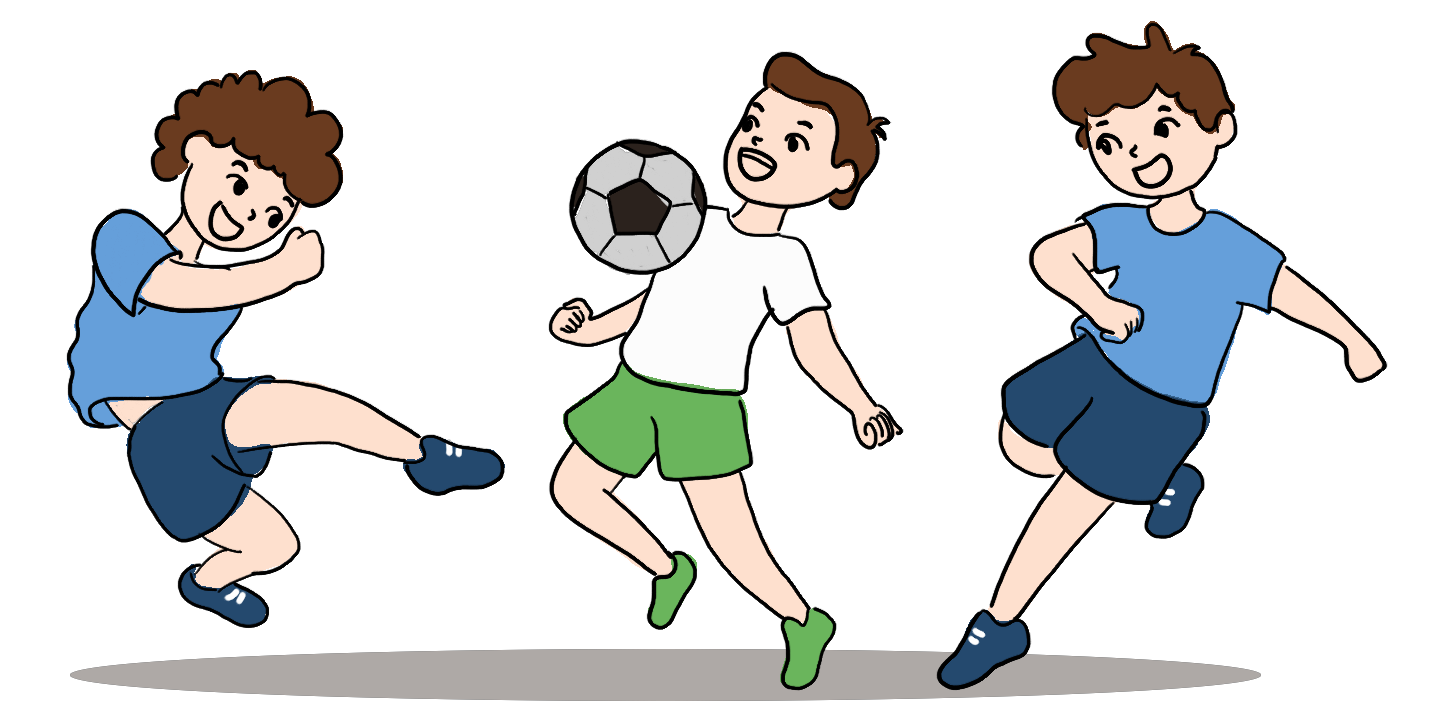
\includegraphics[width=0.85\linewidth]{Pi7_bai5}
%		\vspace*{-10pt}
%	\end{figure}
%	\textit{Lời giải.} Giả sử là đội Xóm Bắc thắng. Khi đó $4$ dự đoán $a)$, $b)$ $c)$ và $d)$ đều đúng, mâu thuẫn với điều kiện đặt ra.
%	\vskip 0.1cm
%	Tiếp theo, giả sử trận đấu kết thúc với tỷ số hoà. Khi đó ta lại có các dự đoán $a)$, $c)$ và $e)$ đều sai, điều này cũng mâu thuẫn với điều kiện đã cho.
%	\vskip 0.1cm
%	Vì vậy, trong trận bóng này đội Xóm Bắc đã thua. Khi đó các dự đoán $c)$ và $d)$ đều sai, và $3$ dự đoán còn lại là đúng. Có nghĩa là: trận đấu không có tỷ số hoà, có ít nhất một trái bóng được đưa vào lưới của đội Xóm Đông, và trong trận bóng có đúng $3$ bàn thắng được ghi. Điều đó có nghĩa là trận bóng kết thúc với tỷ số $1:2$ nghiêng về phía đội Xóm Đông.
%	\vskip 0.1cm
%	$\pmb{6.}$ 	Tại trại hè có $20$ em học sinh tham gia trò chơi Điệp viên tí hon diễn ra trong $2$ tuần. Mỗi Điệp viên tí hon sẽ theo dõi và viết báo cáo tỉ mỉ về sở thích cá nhân của $10$ em khác trong số $20$ em này để nộp cho Sở chỉ huy. Em hãy chứng tỏ rằng có ít nhất $10$ cặp Điệp viên tí hon đã theo dõi lẫn nhau và viết báo cáo về nhau.
%	\begin{figure}[H]
%		\centering
%		\vspace*{-5pt}
%		\captionsetup{labelformat= empty, justification=centering}
%		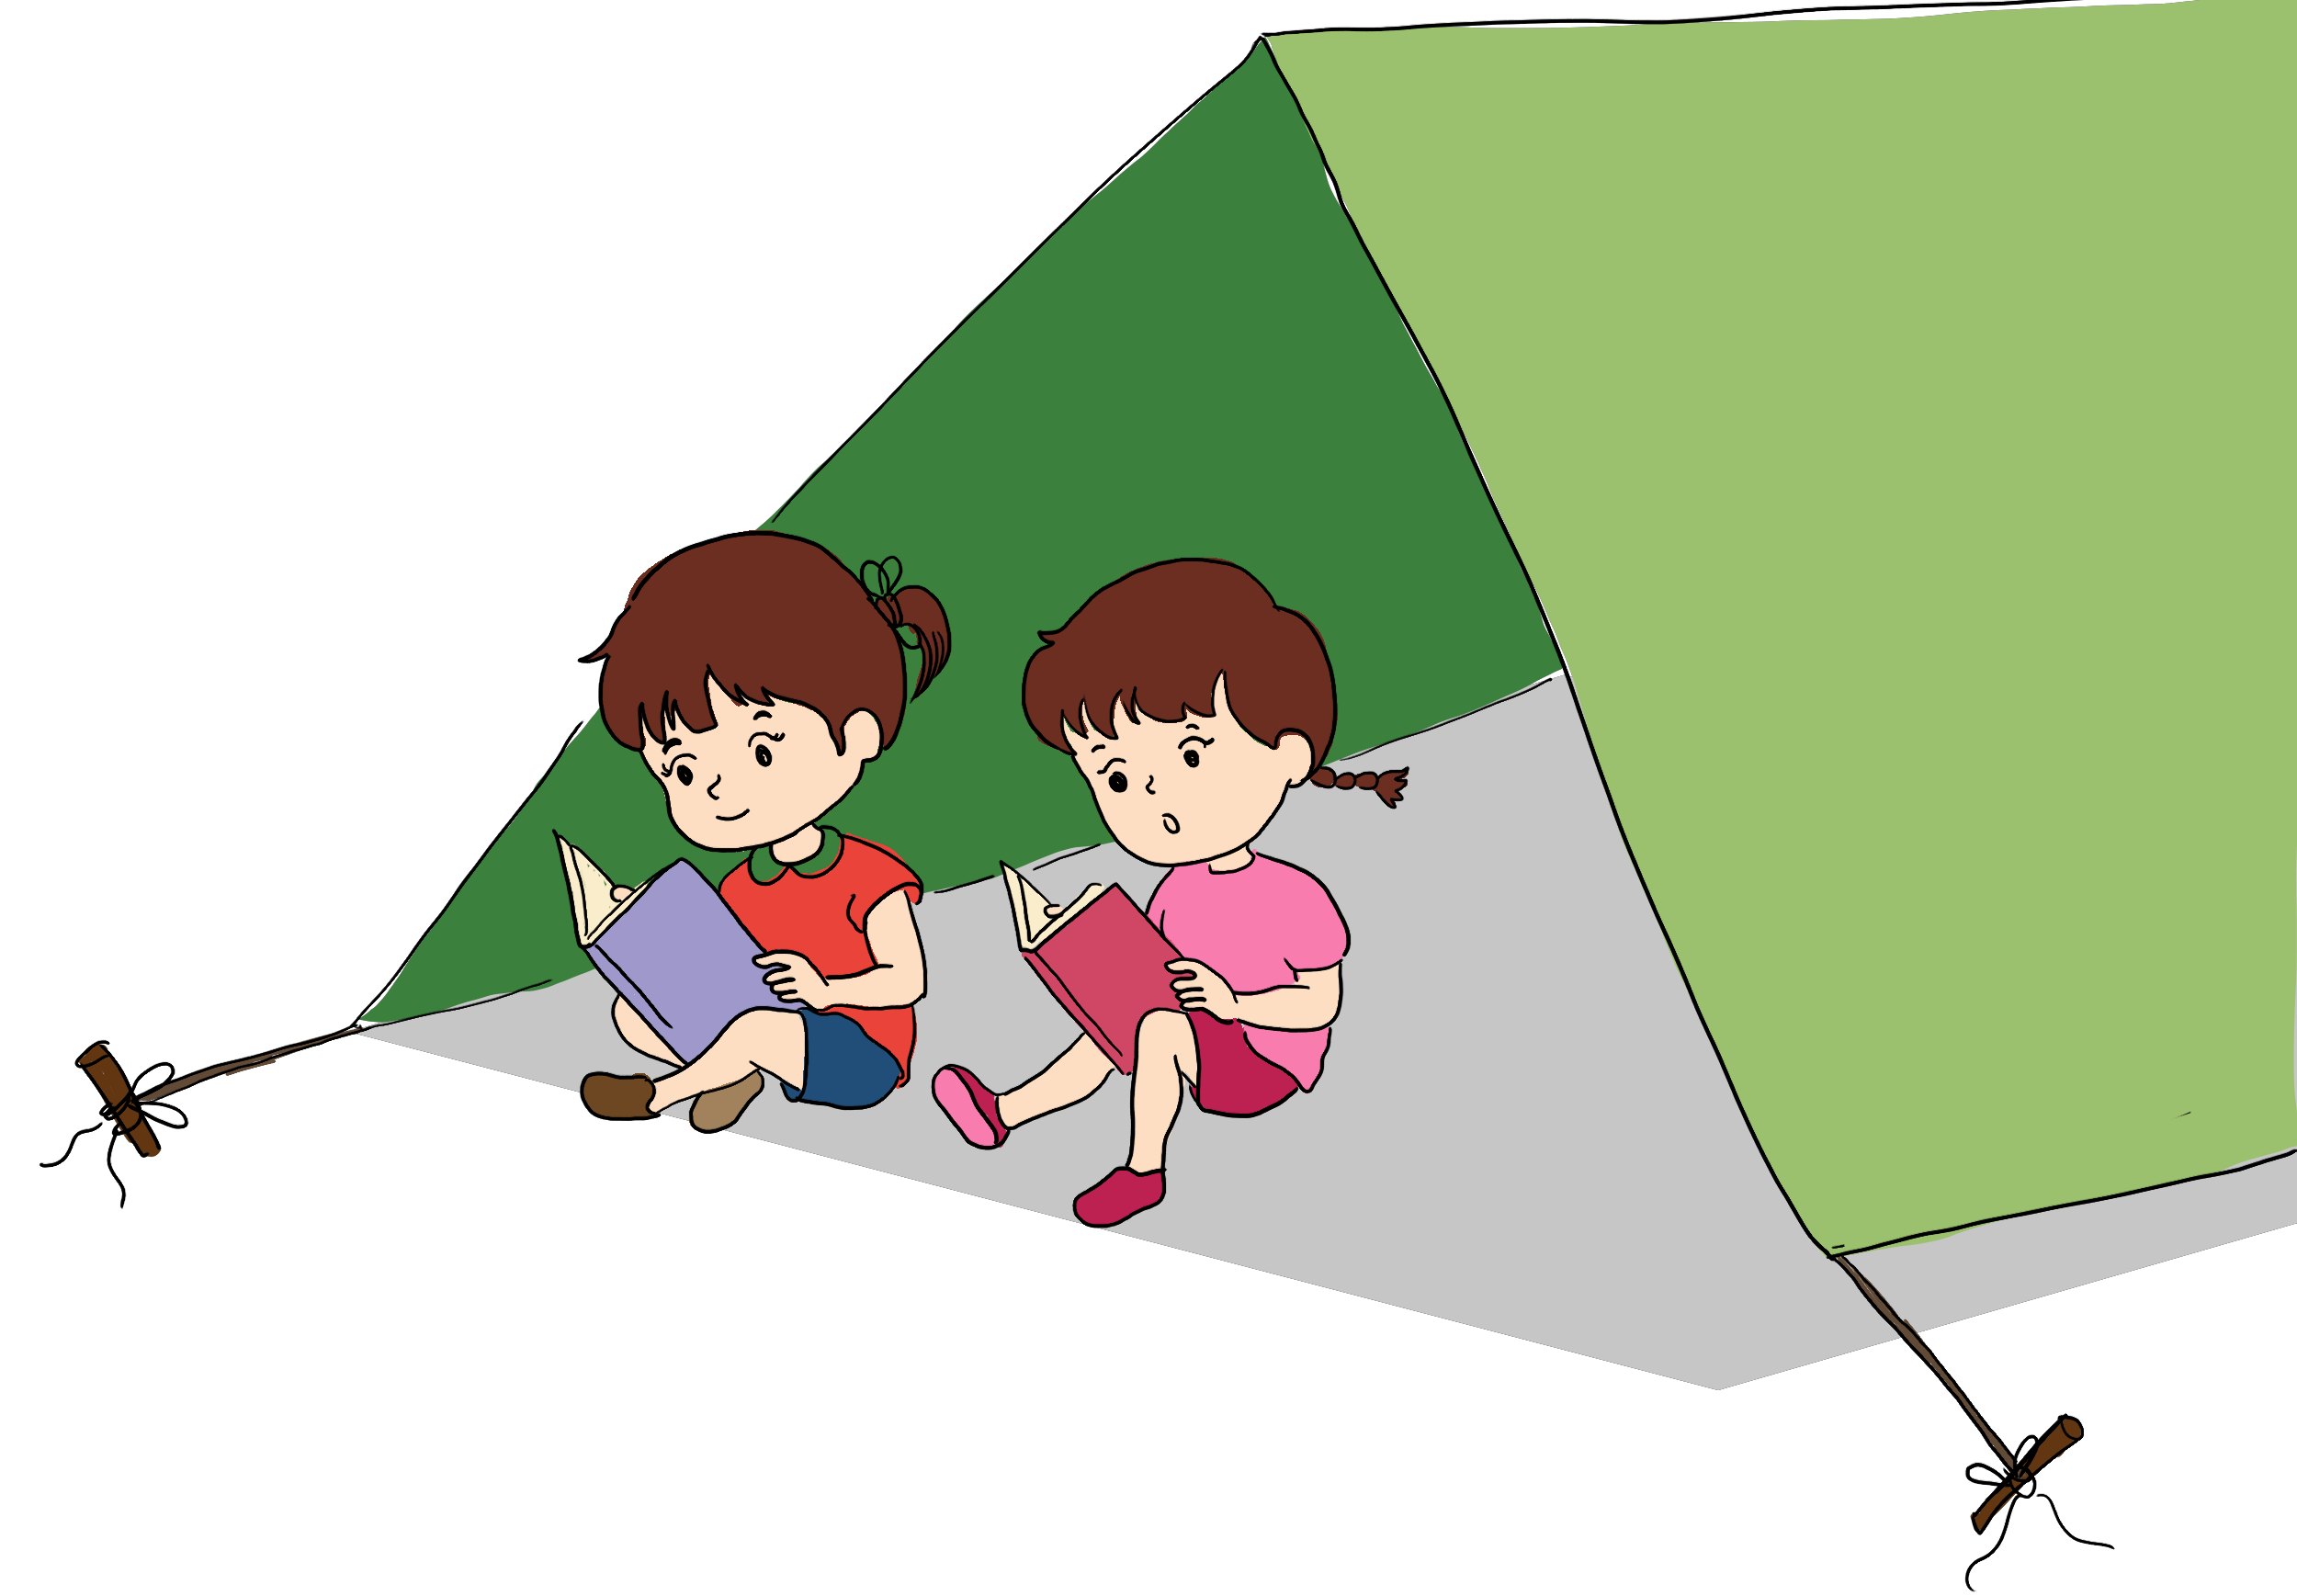
\includegraphics[width=0.75\linewidth]{Pi7_bai6}
%		\vspace*{-15pt}
%	\end{figure}
%	\textit{Lời giải.} Số các cặp Điệp viên tí hon là $\dfrac{20\times 19}{2} = 190$ (cặp). Có tất cả $10\times 20=200$ báo cáo được gửi về Sở chỉ huy vào cuối đợt chơi, suy ra phải có ít nhất $10$ cặp Điệp viên mà hai người trong mỗi cặp báo cáo lẫn nhau về Sở chỉ huy.
%\end{multicols}
%
\newpage
\graphicspath{{../toancuabi/toantienganh/}}
\begingroup
\thispagestyle{toancuabinone}
\blfootnote{$^1$\color{toancuabi}Ottawa, Canada.}
\AddToShipoutPicture*{\put(60,733){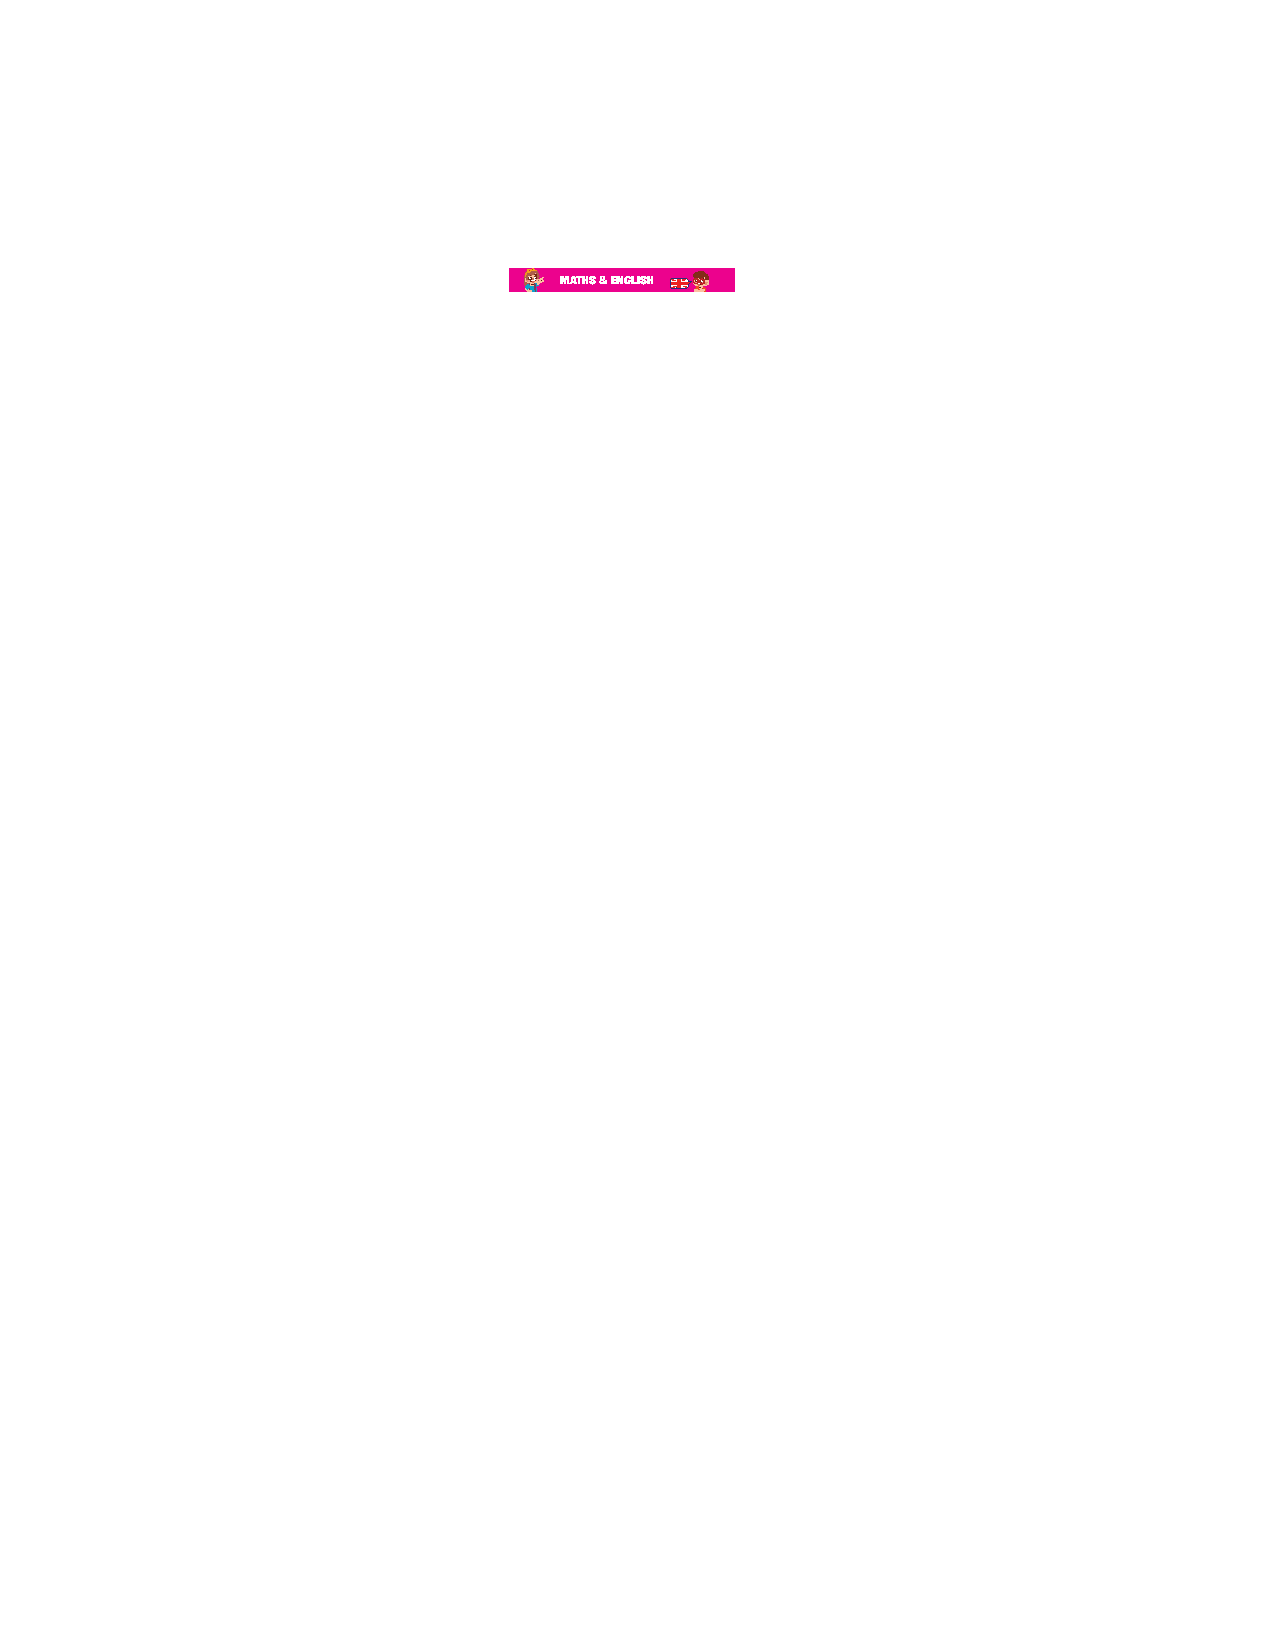
\includegraphics[width=17.2cm]{../mathc.pdf}}}
%\AddToShipoutPicture*{\put(-2,733){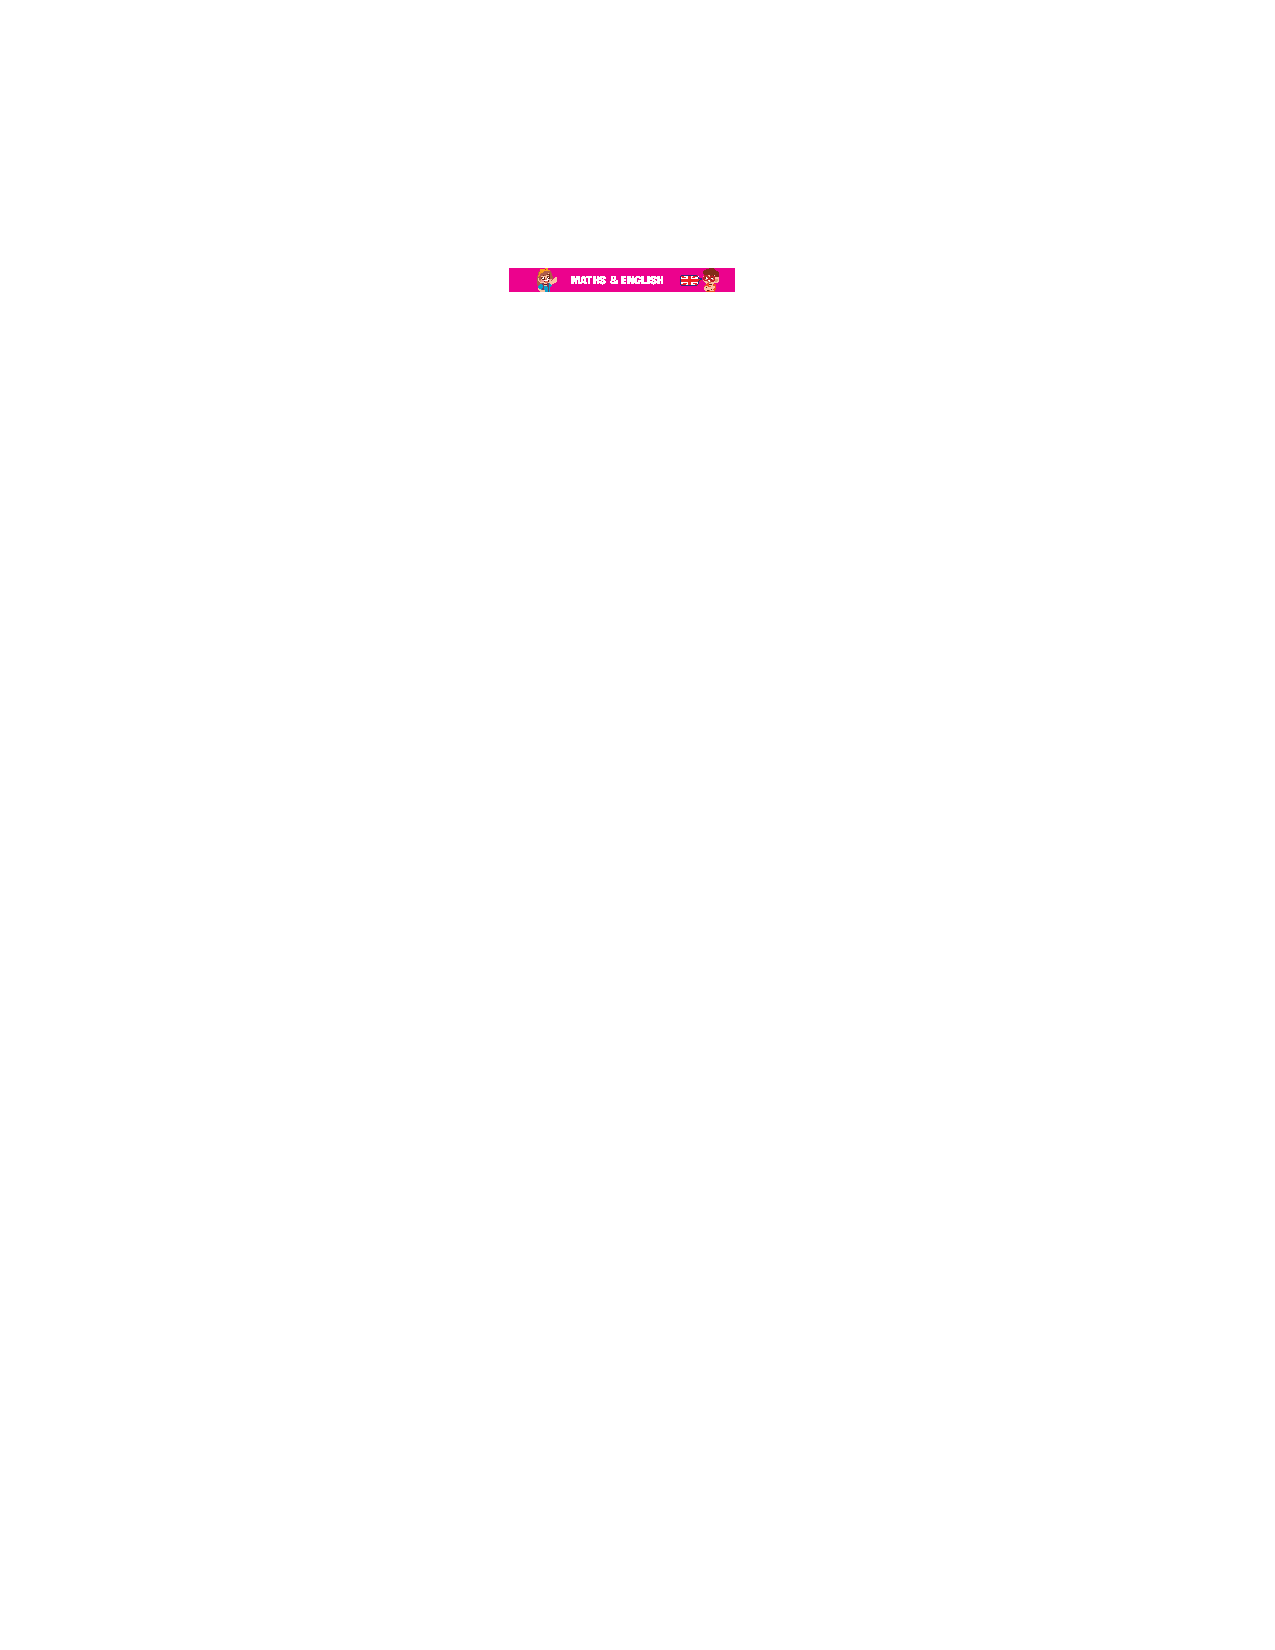
\includegraphics[width=17.2cm]{../mathl.pdf}}} 
\AddToShipoutPicture*{\put(106,675){
\includegraphics[scale=1]{../tieudeb.pdf}}} 
\centering
\endgroup
\vspace*{35pt}

\begin{multicols}{2}
	\setlength{\abovedisplayskip}{6pt}
	\setlength{\belowdisplayskip}{6pt}
	In this article, we will investigate a number of ways to \textit{prove area equality without writing lengthy proof.}
	While it sounds simple, easy, and exciting, it is important that you need to improve your creating thinking in order to 
	first understand the examples, and then use them as tools, guidelines, or ideas to solve the problems.
	\vskip 0.2cm
	\PIbox{
	\textbf{\color{toancuabi}Example $\pmb1$.}
	$E$ is an arbitrary point inside the parallelogram $ABCD,$ prove that
	\begin{align*}
		[AEB] + [CED] = \half [ABCD].
	\end{align*}}
	\begin{figure}[H]
		\vspace*{-5pt}
		\centering
		\captionsetup{labelformat= empty, justification=centering}
		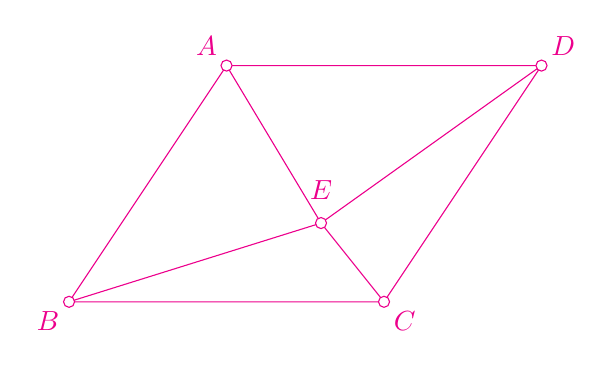
\begin{tikzpicture}[toancuabi]
			\draw (0,0) -- (4,0) -- (6,3) -- (2,3) -- (0,0) -- (3.2,1) -- (4,0) (2,3) -- (3.2,1) -- (6,3);
			\draw[fill=white] (3.2,1) circle (2pt) node [above=5pt] {$E$};
			\draw[fill=white] (2,3) circle (2pt) node [anchor = south east] {$A$};
			\draw[fill=white] (0,0) circle (2pt) node [anchor = north east] {$B$};
			\draw[fill=white] (4,0) circle (2pt) node [anchor = north west] {$C$};
			\draw[fill=white] (6,3) circle (2pt) node [anchor = south west] {$D$};
		\end{tikzpicture}
		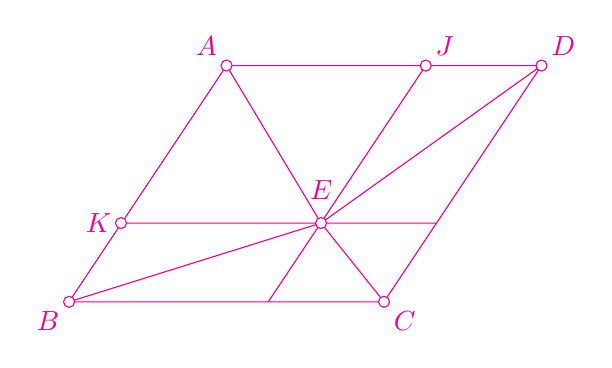
\begin{tikzpicture}[toancuabi]
			\draw (0,0) -- (4,0) -- (6,3) -- (2,3) -- (0,0) -- (3.2,1) -- (4,0) (2,3) -- (3.2,1) -- (6,3) (2.53,0) -- (4.53,3) (0.66,1) --(4.66,1);
			\draw[fill=white] (3.2,1) circle (2pt) node [above=5pt] {$E$};
			\draw[fill=white] (2,3) circle (2pt) node [anchor = south east] {$A$};
			\draw[fill=white] (0,0) circle (2pt) node [anchor = north east] {$B$};
			\draw[fill=white] (4,0) circle (2pt) node [anchor = north west] {$C$};
			\draw[fill=white] (6,3) circle (2pt) node [anchor = south west] {$D$};
			\draw[fill=white] (4.53,3) circle (2pt) node [anchor = south west] {$J$};
			\draw[fill=white] (0.66,1) circle (2pt) node [left] {$K$};
		\end{tikzpicture}
		\vspace*{-10pt}
	\end{figure}
%	\begin{figure}[H]
%		\vspace*{-10pt}
%		\centering
%		\captionsetup{labelformat= empty, justification=centering}
%		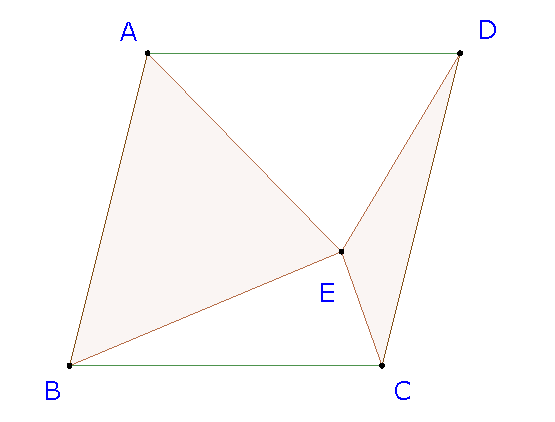
\includegraphics[width= 1\linewidth]{23-24-s3-i-p1.pdf}
%		\vspace*{-20pt}
%	\end{figure}
	\textit{Solution.}
	Draw lines through $E,$ parallel with sides of $ABCD,$ dividing the parallelogram into four smaller parallelograms.
	Any of the smaller parallelogram, say $AKEJ$, consists of a brown triangle from the shaded triangle and a green triangles with the same area.
	Thus, the area of the shaded triangles is the sum of the area of all smaller brown triangles, which is half of the sum of the area of all smaller parallelograms,
	of half of the $ABCD$ parallelogram.
	\vskip 0.1cm
	\textbf{\color{toancuabi}Remark.} Here's how we use the techniques:
	\vskip 0.1cm
	$1.$ First, divide the given figure into smaller figures.
	\vskip 0.1cm
	$3$. Deal with each of them, iif they have the same shape, then work in the same way.
	\vskip 0.1cm
	$3.$ Use all partial results to arrive at the overall result.
	\vskip 0.2cm
%	\begin{figure}[H]
%		\vspace*{-5pt}
%		\centering
%		\captionsetup{labelformat= empty, justification=centering}
%		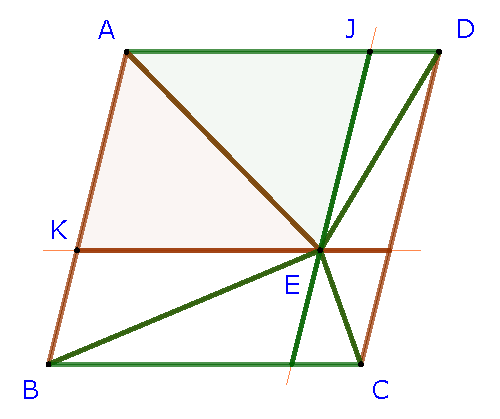
\includegraphics[width= 0.9\linewidth]{23-24-s3-i-p1-s.pdf}
%		\vspace*{-15pt}
%	\end{figure}
	\PIbox{\textbf{\color{toancuabi}Example $\pmb2$.}
	$E$ and $F$ are midpoints of $BC$ and $DA$ in the convex quadrilateral $ABCD,$ prove that
	\begin{align*}
		[AECF] = \half [ABCD].
	\end{align*}}
\begin{figure}[H]
	\vspace*{-5pt}
	\centering
	\captionsetup{labelformat= empty, justification=centering}
	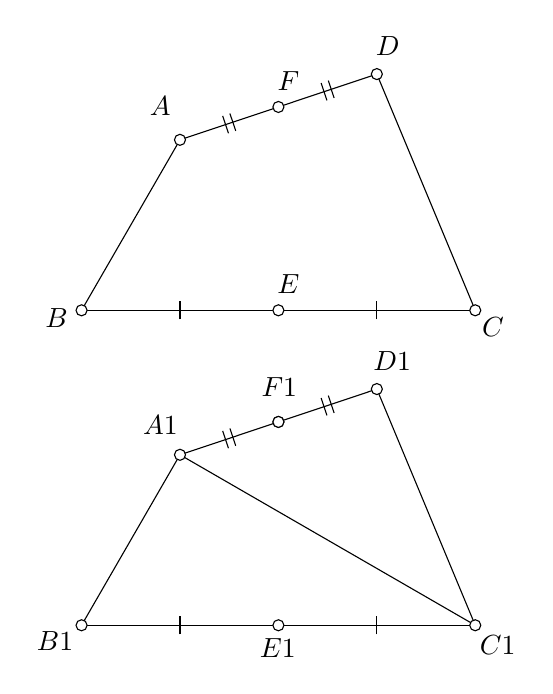
\begin{tikzpicture}
		\draw  (5.,0.)-- (3.75,3.);
		\draw  (5.,-4.)-- (3.75,-1.);
		\draw  (0.,0.)-- (1.25,2.165063509461097);
		\draw  (1.25,2.165063509461097)-- (2.5,2.5825317547305486);
		\draw  (1.7922093978532345,2.468742834111641) -- (1.8658796296660776,2.248156500157986);
		\draw  (1.884120370333924,2.499438764033659) -- (1.957790602146767,2.278852430080004);
		\draw  (2.5,2.5825317547305486)-- (3.75,3.);
		\draw  (3.0422093978532336,2.8862110793810927) -- (3.1158796296660767,2.6656247454274378);
		\draw  (3.134120370333923,2.9169070093031104) -- (3.207790602146766,2.6963206753494555);
		\draw  (5.,-4.)-- (2.5,-4.);
		\draw  (3.75,-4.11628159117254) -- (3.75,-3.8837184088274594);
		\draw  (2.5,-4.)-- (0.,-4.);
		\draw  (1.25,-4.11628159117254) -- (1.25,-3.8837184088274594);
		\draw  (0.,-4.)-- (1.25,-1.8349364905389032);
		\draw  (1.25,-1.8349364905389032)-- (5.,-4.);
		\draw  (5.,0.)-- (2.5,0.);
		\draw  (3.75,-0.11628159117254047) -- (3.75,0.11628159117254047);
		\draw  (2.5,0.)-- (0.,0.);
		\draw  (1.25,-0.11628159117254047) -- (1.25,0.11628159117254047);
		\draw  (1.25,-1.8349364905389032)-- (2.5,-1.4174682452694516);
		\draw  (1.7922093978532345,-1.53125716588836) -- (1.8658796296660776,-1.7518434998420143);
		\draw  (1.884120370333924,-1.5005612359663414) -- (1.957790602146767,-1.7211475699199956);
		\draw  (2.5,-1.4174682452694516)-- (3.75,-1.);
		\draw  (3.0422093978532336,-1.1137889206189073) -- (3.1158796296660767,-1.3343752545725616);
		\draw  (3.134120370333923,-1.0830929906968887) -- (3.207790602146766,-1.303679324650543);
			\draw [fill=white] (0.,0.) circle (2.0pt);
			\draw (-0.3177952991732108,-0.09743478291470092) node {$B$};
			\draw [fill=white] (5.,0.) circle (2.0pt);
			\draw (5.224960546717885,-0.21371637408724142) node {$C$};
			\draw [fill=white] (2.5,0.) circle (2.0pt);
			\draw (2.6280050105311474,0.3289310513846141) node {$E$};
			\draw [fill=white] (1.25,2.165063509461097) circle (2.0pt);
			\draw (1.0000627341155812,2.5964220792491535) node {$A$};
			\draw [fill=white] (3.75,3.) circle (2.0pt);
			\draw (3.8877222482336693,3.3522524218706664) node {$D$};
			\draw [fill=white] (2.5,2.5825317547305486) circle (2.0pt);
			\draw (2.6280050105311474,2.906506322375928) node {$F$};
			\draw [fill=white] (0.,-4.) circle (2.0pt);
			\draw (-0.33717556436863416,-4.206051004344464) node {$B1$};
			\draw [fill=white] (5.,-4.) circle (2.0pt);
			\draw (5.283101342304154,-4.244811534735311) node {$C1$};
			\draw [fill=white] (3.75,-1.) circle (2.0pt);
			\draw (3.94586304381994,-0.6400822083865565) node {$D1$};
			\draw [fill=white] (2.5,-4.) circle (2.0pt);
			\draw (2.492343154163184,-4.283572065126157) node {$E1$};
			\draw [fill=white] (1.25,-1.8349364905389032) circle (2.0pt);
			\draw (1.0000627341155812,-1.4540533465943397) node {$A1$};
			\draw [fill=white] (2.5,-1.4174682452694516) circle (2.0pt);
			\draw (2.5117234193586073,-0.9695467167087544) node {$F1$};
			\draw [fill=white] (2.5,-1.4174682452694516) circle (2.0pt);
	\end{tikzpicture}
	\vspace*{-10pt}
\end{figure}

	\textit{Solution.}
	Connect $AC.$ Since $E$ is midpoint of $BC,$ thus the triangles $ABE$ and $AEC$ have the same area.
	Similarly triangles $CDF$ and $CFA$ have the same area. Thus the area of $AECF$ is half of $ABCD.$
	\vskip 0.2cm
%	\begin{figure}[H]
%		\vspace*{-5pt}
%		\centering
%		\captionsetup{labelformat= empty, justification=centering}
%		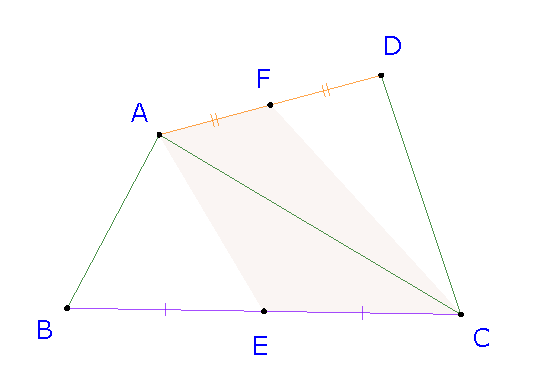
\includegraphics[width= 1\linewidth]{23-24-s3-i-p2-s.pdf}
%		\vspace*{-10pt}
%	\end{figure}
	\PIbox{\textbf{\color{toancuabi}Example $\pmb3$.}
		$I$ is an arbitrary point on the diagonal $BD$ in parallelogram $ABCD.$
		Lines through $I$ parallel with the sides of $ABCD$ intersect $AB,$ $BC,$ $CD,$ and $DA$ at $E, F, G,$ and $H,$ respectively.
		\begin{align*}
			[AEIH] = [FCGI].
		\end{align*}}
	\begin{figure}[H]
		\vspace*{-5pt}
		\centering
		\captionsetup{labelformat= empty, justification=centering}
		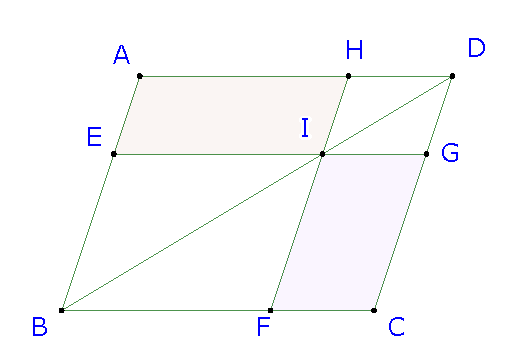
\includegraphics[width= 1\linewidth]{23-24-s3-i-p3.pdf}
		\vspace*{-10pt}
	\end{figure}
	\textit{Solution.}
	First, since $BD$ is the diagonal in parallelogram $ABCD,$ $[ABD] = [BCD].$
	Now, $BEIF$ is also a parallelogram, thus $[BEI] = [BFI],$ similarly $[HID] = [IGD].$
	Therefore 
	\begin{align*}
		[AEIH] &= [ABD] - [BEI] - [HID] \\
		&= [BCD] - [BFI] - [IGD] \\
		&= [FCGI].
	\end{align*}
	\begin{figure}[H]
		\vspace*{-5pt}
		\centering
		\captionsetup{labelformat= empty, justification=centering}
		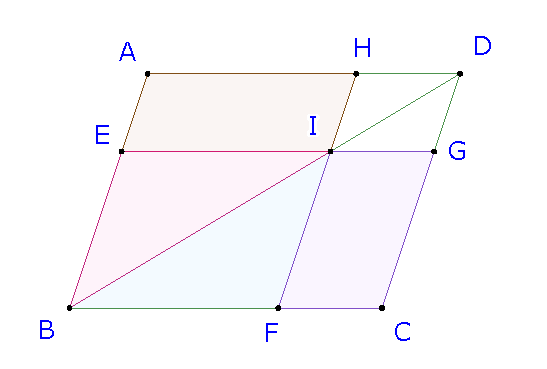
\includegraphics[width= 1\linewidth]{23-24-s3-i-p3-s.pdf}
		\vspace*{-10pt}
	\end{figure}
	\PIbox{\textbf{\color{toancuabi}Example $\pmb4$.} 
	$G, H$ are midpoints of $BC, CD$ in th regular hexagon $ABCDEF.$
	$EG$ and $FH$ intersect at $I.$ Prove that
	\begin{align*}
		[GCHI] = [EFI].
	\end{align*}}
	\begin{figure}[H]
		\vspace*{-5pt}
		\centering
		\captionsetup{labelformat= empty, justification=centering}
		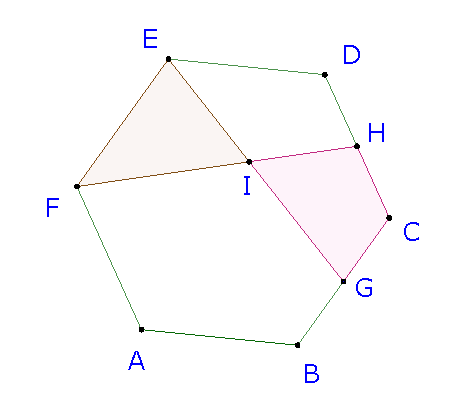
\includegraphics[width= 1\linewidth]{23-24-s3-i-p4.pdf}
		\vspace*{-10pt}
	\end{figure}
	\textit{Solution.}
		It is easy to see that the quadrilaterals $GCDE$ and $HDEF$ are congruent, thus have the same area, or $[GCDE] = [HDEF].$
		Taking $HDEI$ away, we have $[GCHI] = [EFI].$ 
	\vskip 0.2cm
	\PIbox{\textbf{\color{toancuabi}Example $\pmb5$.}
		$E, F, G,$ and $H$ are midpoints the sides in the convex quadrilateral $ABCD.$
		Prove that
		\begin{align*}
			[EFGH] = \half [ABCD].
		\end{align*}}
	\begin{figure}[H]
		\vspace*{-5pt}
		\centering
		\captionsetup{labelformat= empty, justification=centering}
		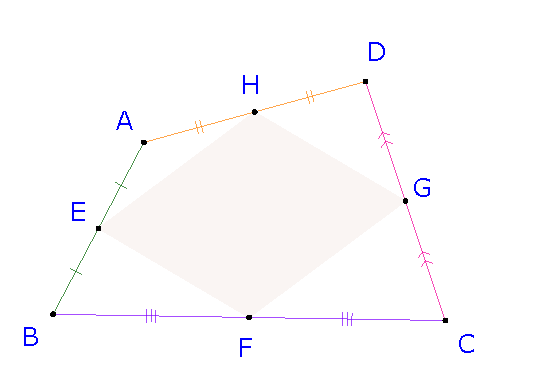
\includegraphics[width= 1\linewidth]{23-24-s3-i-p5.pdf}
		\vspace*{-10pt}
	\end{figure}
	\textit{Solution.}
		$EH$ is the mid-segment (the segment connecting two midpoints) in $\triangle ABD,$ therefore $[AEH] = \frac{1}{4}[ABD].$
		Similarly $[BEF] = \frac{1}{4}[ABC],$ $[CFG] = \frac{1}{4}[BCD],$ and $[GDH] = \frac{1}{4}[CDA],$ therefore:
		\begin{align*}
			&[AEH] + [BEF] + [CFG] + [GDH] \\
			&= \half [ABCD]\\
			 \Rightarrow  &[EFGH] = \half [ABCD].
		\end{align*} 
\end{multicols}

%	\newpage 
%
	\setcounter{figure}{0}
	\thispagestyle{hoccungpinone}
\pagestyle{hoccungpi}
\everymath{\color{hoccungpi}}
\graphicspath{{../hoccungpi/pic/}}
\blfootnote{$^{1}$\color{hoccungpi}Lớp $12$ Toán $1$, Trường THPT Amsterdam, Hà Nội.}
\blfootnote{$^{2}$\color{hoccungpi}Khoa Toán -- Tin, Đại học Sư Phạm Hà Nội.}
\begingroup
\AddToShipoutPicture*{\put(0,616){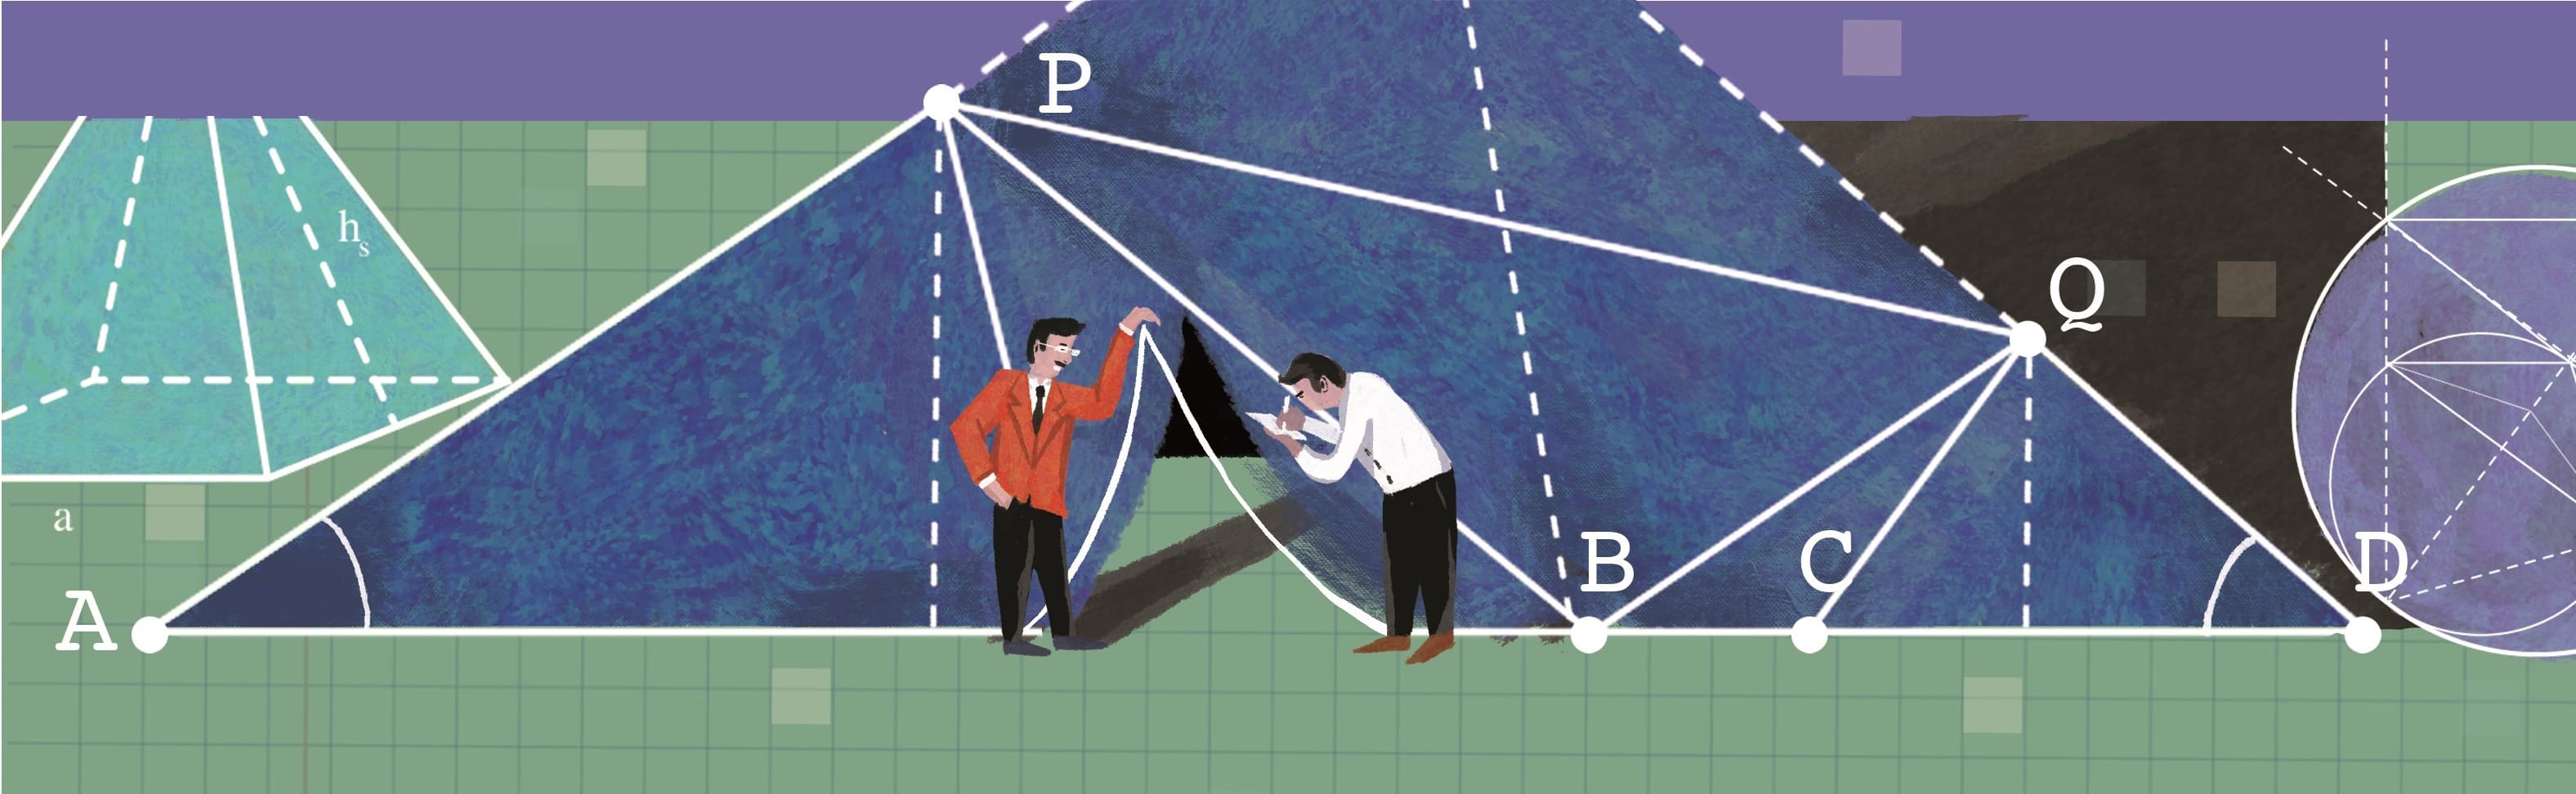
\includegraphics[width=19.3cm]{../bannerhoccungpi}}}
\AddToShipoutPicture*{\put(80,550){
\includegraphics[scale=1]{../tieude1.pdf}}}
\centering
\endgroup

\vspace*{160pt}

\begin{multicols}{2}
$\pmb{1.}$ \textbf{\color{hoccungpi}Giới thiệu}
\vskip 0.1cm
Định lý Fermat lớn nói về sự không tồn tại bộ ba số nguyên $a,b,c$ khác $0$ sao cho $a^n+b^n=c^n$ với $n\ge 3$ là số nguyên dương, đã được Andrew Wiles [$5$] chứng minh vào năm $1995$, nhưng ít ai biết rằng có một định lý ``Fermat" tương tự cho đa thức đã được chứng minh trước đó hàng chục năm trước, tức không tồn tại ba đa thức $f(x),g(x),h(x)$ với hệ số thực, ít nhất một đa thức khác đa thức hằng, đôi một không có nghiệm chung sao cho $f(x)^n+g(x)^n=h(x)^n,$ với $ n\ge 3$ là một số nguyên dương cho trước.
\vskip 0.1cm
Định lý Fermat cho đa thức là hệ quả của Định lý Mason -- Stothers, đầu tiên được Stothers [$4$] chứng minh vào năm $1981$, và Mason [$3$] độc lập phát hiện ra sau đó ít lâu. Các chứng minh đó nhìn chung là phức tạp, không sơ cấp. Năm $2000$, Snyder [$2$] đã đưa ra một chứng minh mới, chỉ với các kiến thức toán phổ thông cho định lý này. Trong bài viết này, chúng tôi giới thiệu chứng minh của Snyder và sau đó áp dụng Định lý Mason--Stothers để chứng minh Định lý Fermat cho đa thức và một số kết quả liên quan khác.
\vskip 0.1cm 
$\pmb{2. }$ \textbf{\color{hoccungpi}Định lý Mason -- Stothers}
\vskip 0.1cm
	\textbf{\color{hoccungpi}Định lý} $\pmb{1}$ (Mason -- Stothers)\textbf{\color{hoccungpi}.} 
\textit{	Cho $a(x),$ $b(x)$ và $c(x)$ là các đa thức khác đa thức hằng, với hệ số thực, đôi một không có nghiệm phức chung và thỏa mãn: $a(x) + b(x) = c(x)$. Khi đó
	\begin{align*}
		\deg(c) \le n_0{(abc)} - 1,
	\end{align*}
	trong đó ta ký hiệu $n_0(f)$ là số nghiệm phức phân biệt của đa thức $f(x)$ và $\deg(f)$ là bậc của đa thức $f(x).$}
	\vskip 0.1cm
	Để chứng minh Định lý này, ta cần Bổ đề sau:
	\vskip 0.1cm
	\textbf{\color{hoccungpi}Bổ đề} $\pmb{1.}$
	\textit{Cho $f(x)$ là một đa thức với hệ số thực, khác đa thức $0$.  Khi đó,
	\begin{align*}
		\deg(f) \le \deg(f,f') + n_0(f),
	\end{align*}
	trong đó ta ký hiệu $(f,f')$ là ước chung lớn nhất của hai đa thức $f(x)$ và $f'(x)$ ($f'(x)$ là đa thức đạo hàm của đa thức $f(x)$).} 
	\vskip 0.1cm
	\textit{Chứng minh.}
	Gọi $\alpha_1, \alpha_2, \ldots,  \alpha_m $ là các nghiệm phức phân biệt của $f(x)$ với các bội $a_1, a_2, \ldots , a_m$ tương ứng. Khi đó, ta có phân tích
	\begin{align*}
		f(x) \!=\! a(x \!-\! \alpha_1)^{a_1}(x \!-\! \alpha_2)^{a_2}\ldots (x \!-\! \alpha_m)^{a_m},
	\end{align*}
	với $a\in \mathbb{R}$ và $a_1+a_2+\cdots+a_m=\deg f(x).$
	Ta có, theo công thức Leibniz, đạo hàm của $f(x)$ được cho bởi:
	\begin{align*}
		&f'(x) \\
		=\,\,& aa_1(x - \alpha_1)^{a_1-1}(x - \alpha_2)^{a_2} \ldots (x - \alpha_m)^{a_m}  \\
		&\!+  a(x - \alpha_1)^{a_1} [(x - \alpha_2)^{a_2}\ldots(x - \alpha_m)^{a_m}]'.
	\end{align*}
	Suy ra, với mỗi $i=1, 2, \ldots, m$, đa thức $(x-\alpha_i)^{a_i-1}$ cùng là ước của $f(x)$ và $f'(x)$.
	Do đó 
	\begin{align*}
		&(x - \alpha_1)^{a_1 - 1}(x - \alpha_2)^{a_2 - 1} \ldots \\
		&(x - \alpha_m)^{a_m - 1} \mid (f,f').
	\end{align*} 
	Vì $f(x)$ là đa thức khác đa thức hằng nên $f'(x)$ khác đa thức $0$ và do đó $(f, f')$ cũng khác đa thức $0$. Suy ra
	\begin{align*}
		&\deg((x - \alpha_1)^{a_1 - 1}(x - \alpha_2)^{a_2 - 1}\ldots \\
		&(x - \alpha_m)^{a_m - 1}) \leq \deg(f,f'),
	\end{align*} 
	hay 
	\begin{align*}
		&(a_1-1)+(a_2-1)+\cdots+(a_m-1)\\
		\leq \,&\deg (f,f').
	\end{align*}
	Suy ra
	\begin{align*}
		\deg(f) - n_0(f) \leq \deg(f,f').
	\end{align*}
	Vậy bổ đề được chứng minh
	\vskip 0.1cm
	\textit{Chứng minh Định lý} $1.$
	Từ giả thiết 
	\begin{align*}
		a + b = c, \tag{$1$} 
	\end{align*}
	bằng cách lấy đạo hàm hai vế, ta được
	\begin{align*}
		a' + b' = c'. \tag{$2$}
	\end{align*}
	Nhân ($1$) với $a'$ và nhân ($2$) với $a$ và trừ vế với vế, ta được
	\begin{align*}
		a'b - ab' = a'c - ac'.
	\end{align*}
	Suy ra $(a,a'), (b,b')$ và $(c,c')$ đều là ước của $a'b - ab'$.
	\vskip 0.1cm
	Do các đa thức $a,b,c$ đôi một không có nghiệm phức chung nên các đa thức $(a,a'), (b,b')$ và $(c,c')$ cũng đôi một không có nghiệm phức chung. Suy ra
	\begin{align*}
		(a,a')(b,b')(c,c') \mid a'b - ab'.
	\end{align*}
	Hơn nữa, ta có $a'b - ab'\ne 0$. Thật vậy, nếu $ a'b - ab'= 0$ thì $\left(\dfrac{a}{b}\right)'=0$ hay $\dfrac{a}{b}$ là hằng số. Do đó $a$ và $b$ có nghiệm chung (mâu thuẫn với giả thiết).
	Vì vậy, 
	\begin{align*}
		\deg ((a,a')(b,b')(c,c'))\leq \deg(a'b - ab').
	\end{align*} 
	Mặt khác, hiển nhiên ta có 
	\begin{align*}
		\deg(a'b-ab')&\leq \max\{\deg(a'b),\deg(ab')\}\\
			&=\deg(a)+\deg(b)-1.
	\end{align*}
	Vì thế,
	\begin{align*}
		&\deg(a,a') + \deg(b,b') + \deg(c,c') \\
		\leq \,&\deg(a) + \deg(b) - 1.
	\end{align*}
	Chuyển vế bất đẳng thức này và cộng với $\deg (c)$ vào hai vế, ta được 
	\begin{align*}
		\deg(c) \leq& \deg(a) - \deg(a,a') + \deg(b) \\
		&\!\!\!-\! \deg(b,b') \!+\! \deg(c) \!-\! \deg(c,c')\!-\!1.
	\end{align*} 
	Cuối cùng, áp dụng Bổ đề $1$, ta có:
	\begin{align*}
		&\deg(a) - \deg(a,a') \leq n_0{(a)},\\
		&\deg(b) - \deg(b,b') \leq n_0{(b),}\\
		&\deg(c) - \deg(c,c') \leq n_0{(c)},
	\end{align*}
	Từ đó suy ra 
	\begin{align*}
		\deg(c) &\le n_0{(a)} + n_0{(b)} + n_0{(c)} - 1 \\
		&= n_0{(abc)} - 1.
	\end{align*}
	$\pmb{3.}$ \textbf{\color{hoccungpi}Định lý Fermat cho đa thức}
	\vskip 0.1cm
	Áp dụng Định lý Mason -- Stothers, chúng ta có một số kết quả đáng lưu ý. Trước hết, ta có kết quả sau đây:
	\vskip 0.1cm
	\textbf{\color{hoccungpi}Định lý} $\pmb{2}$  (Davenport [$1$])\textbf{\color{hoccungpi}.} \textit{Cho $f(x),g(x)$ là các đa thức với hệ số thực, khác đa thức hằng, đôi một không có nghiệm phức chung. Đặt $h(x)=(f(x))^3-(g(x))^2$ và giả sử $h(x)$ khác là đa thức $0$. Khi đó, $\deg (f) \leq 2\deg (h)-2$.}
	\vskip 0.1cm
	\textit{Chứng minh.}
	Do $f(x)$ và $g(x)$ là các đa thức không có nghiệm chung và $h = f^3 - g^2$ nên $h, f^3$ và $g^2$ đôi một không có nghiệm chung.  Áp dụng Định lý Mason -- Stothers cho ba đa thức $ g^2, h$ và $f^3,$ ta có:
	\begin{align*}
		\deg(f^3) \leq n_0{(g^2hf^3)} - 1,
	\end{align*}
	hay 
	\begin{align*}
		3\deg (f)\leq n_0{(ghf)}-1\leq \deg(ghf) - 1.
	\end{align*}
	Mà $\deg(ghf)= \deg(g) + \deg(h) +\deg(f)$, nên 
	\begin{align*}
		&3\deg(f)\\
		\leq \, &\deg(g) + \deg(h) +\deg(f)-1. \tag{$3$}
	\end{align*}
	Chứng minh tương tự, ta có:
	\begin{align*}
		&2\deg(g) \\
		\leq \, &\deg(g) + \deg(h) +\deg(f) - 1.\tag{$4$}
	\end{align*}
	Kết hợp ($3$) và ($4$), ta được
	\begin{align*}
		&3\deg(f) + 2\deg(g) \\
		\leq \,&2(\deg(g) + \deg(h) +\deg(f) - 1)
	\end{align*}
	hay $\deg(f) \leq 2\deg(h) - 2.$ Ta có điều phải chứng minh.
	\vskip 0.1cm
	\textbf{\color{hoccungpi}Hệ quả} $\pmb{1.}$
	\textit{Không tồn tại hai đa thức với hệ số thực $f(x)$ và $g(x)$, khác đa thức hằng sao cho $f^3-g^2$ là đa thức hằng khác đa thức $0$.}
	\vskip 0.1cm
	Như đã đề cập đến trong phần đầu của bài viết, định lý Mason--Stothers có thể được sử dụng để chứng minh phiên bản đa thức của định lý Fermat lớn.
	\vskip 0.1cm
	\textbf{\color{hoccungpi}Định lý} $\pmb{3}$ (Định lý Fermat cho đa thức)\textbf{\color{hoccungpi}.} \textit{Với mọi nguyên $n\ge 3$, không tồn tại ba đa thức $f(x),g(x),h(x)$, với hệ số thực, đôi một không có nghiệm phức chung, trong đó ít nhất một đa thức khác đa thức hằng, sao cho $f^n+g^n=h^n$.}
	\vskip 0.1cm
	\textit{Chứng minh.}
	Giả sử ngược lại, $f^n+g^n=h^n$. Áp dụng định lý Mason--Stothers cho $3$ đa thức $f^n, g^n$ và $h^n$, ta có:
	\begin{align*}
		&\max\{\deg(f^n), \deg(g^n), \deg(h^n)\} \\
		\le\, &n_0{(f^ng^nh^n)} - 1 = n_0{(fgh)} - 1 \\
		\le\, &\deg(f) + \deg(g) + \deg(h) - 1.
	\end{align*}
	Để ý rằng
	\begin{align*}
		&\dfrac{n}{3}(\deg(f) + \deg(g) + \deg(h)) \\
		=    \,&\dfrac{1}{3}(\deg(f^n) + \deg(g^n) + \deg(h^n)) \\
		\le\,& \max\{\deg(f^n), \deg(g^n), \deg (h^n).
	\end{align*}
	Do đó, nếu ta đặt $d=\deg(f) + \deg(g) + \deg(h)$ thì bằng cách kết hợp với bất đẳng thức thu được ở trên, ta có:
	\begin{align*}
		\dfrac{nd}{3} \le d - 1.
	\end{align*}
	Suy ra, $3 < d(3-n).$ Do ít nhất một trong các đa thức $f, g, h$ khác hằng nên $d >0$; điều này, kết hợp với giả thiết $n\ge 3$, dẫn đến $3\le 0$, mâu thuẫn. 
	\vskip 0.1cm
	Với chứng minh tương tự, ta có thể chỉ ra được hệ quả sau đây, mà nội dung của nó là một bài toán trong tuyển tập Các kỳ thi Toán Rumani (RMC) năm $2019$.
	\vskip 0.1cm
	\textbf{\color{hoccungpi}Hệ quả} $\pmb{2.}$ \textit{Cho các số nguyên $m,n\ge 3$ và $f,g$ là các đa thức khác hằng với hệ số thực, trong đó ít nhất một đa thức có bậc lớn hơn hoặc bằng $2$. Giả sử $\deg (f^m-g^n)<\min \{m,n\}$. Khi đó $f^m=g^n$.}
	\vskip 0.1cm
	\textbf{\color{hoccungpi}Nhận xét.}
	Định lý Mason -- Stothers cũng đúng khi ta xét các đa thức với hệ số phức. Từ đó ta suy ra Định lý Davenport và Định lý Fermat cho đa thức cũng đúng với đa thức với hệ số phức.
	\vskip 0.1cm
	Để kết thúc, chúng ta trình bày một mở rộng của Định lý $3$.
	\vskip 0.1cm
	\textbf{\color{hoccungpi}Định lý} $\pmb{4.}$ \textit{Cho các số nguyên dương $m,n,p$ thỏa mãn $m\leq n\leq p$. Khi đó phương trình đa thức $f(x)^m+g(x)^n=h(x)^p$ có nghiệm $f,g,h$ là các đa thức với hệ số phức, đôi một không có nghiệm chung, ít nhất một trong ba đa thức khác đa thức hằng nếu và chỉ nếu $(m,n,p)$ có một trong dạng sau: $(1,a,b), a,b\ge 1$; $(2,2,a), a\ge 2$; $(2,3,3); (2,3,4); (2,3,5)$.}
	\vskip 0.1cm
	\textit{Chứng minh.}
	Trước hết, dễ thấy rằng nếu trong $m, n, p$ có một số bằng $1$ thì phương trình rõ ràng có nghiệm, chẳng hạn nếu $m=1$, với $g(x),h(x)$ là hai đa thức khác đa thức hằng tùy ý, không có nghiệm chung thì bằng cách đặt $f(x)=h(x)^p-g(x)^m$, ta có $f(x), g(x), h(x)$ thỏa mãn phương trình.
	\vskip 0.1cm
	Vì vậy, ta chỉ cần xét trường hợp $ 2 \le m \le n \le p$. Gọi $a, b, c$ lần lượt là bậc của các đa thức $f, g$ và $h$. Khi đó, theo Định lý Mason -- Stothers, ta có
	\begin{align*}
		ma \le a + b + c - 1, \tag{$5$}\\
		nb \le a + b + c - 1, \tag{$6$}\\
		pc \le a + b + c - 1. \tag{$7$}
	\end{align*}
	Cộng vế với vế của ($5$), ($6$) và ($7$) ta được
	\begin{align*}
		m(a+ b + c) &\le ma + nb + pc \\
		&\le 3(a + b + c) - 3.
	\end{align*}
	Suy ra, $m < 3.$ Mặt khác, $2 \le m$ nên $m = 2.$ Khi này, bất đẳng thức ($5$) trở thành:
	\begin{align*}
		a \le b + c - 1. \tag{$8$} 
	\end{align*}
	Cộng các bất phương trình ($6$), ($7$) và  ($8$) theo vế, ta có:
	\begin{align*}
		nb + pc \le 3(b + c) + a - 3. \tag{$9$}
	\end{align*}
	Mặt khác, vì $n \le p$ nên từ bất đẳng thức ($8$) và ($9$), ta có:
	\begin{align*}
		n(b + c) &\le nb + pc \le 3(b + c) + a - 3 \\
		&\le 4(b + c) - 4. \tag{$10$}
	\end{align*}
	Từ đó, $n < 4$. Kết hợp với $n \ge 2$,  ta suy ra $n = 2$ hoặc $n = 3.$
	\vskip 0.1cm
	Với $n = 2$, ta thấy rằng với mọi giá trị của $p\ge 2$ thì tồn tại ba đa thức $f, g, h$ thỏa mãn phương trình của định lý. Chẳng hạn, với
	\begin{align*}
		&f(x) = \dfrac{x^p+1}{2},\\
		& g(x) = -i\left( \dfrac{x^p-1}{2}\right),\\
		&h(x) = x^2,
	\end{align*}
	thì $f^2+g^2=h^p.$
	\vskip 0.1cm
	Với $n = 3$ thì bất đẳng thức ($6$) trở thành
	\begin{align*}
		2b \le a + c - 1. \tag{$11$}
	\end{align*}
	Kết hợp ($8$) và ($11$), ta được 
	$b \le 2c - 2.$ Từ đó,  ($8$) dẫn đến $a\le 3c - 3.$ Từ đó, ($7$) dẫn đến
	\begin{align*}
		pc &\le a + b + c - 1\\
		&\le 3c - 3 + 2c - 2 + c -1=6c-6.
	\end{align*}
	Suy ra $p \le 5.$ Mà $p\ge n$ nên $p\in \{3;4;5\}.$
	\vskip 0.1cm
	Với $p = 3$, ta có thể chọn
	\begin{align*}
		&f(x) = \sqrt[4]{432}e^{\frac{i\pi}{4}}(x^5-x),\\
		&g(x) = x^4  -2i\sqrt{3}x^2 + 1,\\
		&h(x) = x^4 + 2i\sqrt{3} x^2+ 1
	\end{align*}
	để có $f^2+g^3=h^3.$
	\vskip 0.1cm
	Với $p = 4$, ta có thể chọn 
	\begin{align*}
		&f(x) = x^{12} - 33x^8 - 33x^4 + 1,\\
		&g(x) = -(x^8 + 14x^3 + 1),\\
		&h(x) = \sqrt[4]{108} e^{\frac{i\pi}{4}} (x^5 - x)
	\end{align*}
	để có $f^2+g^3=h^4.$
	\vskip 0.1cm
	Với $p = 5$, ta có thể chọn 
	\begin{equation*}
		\begin{array}{l}
			\resizebox{1\linewidth}{!}{$f(x) =\frac{x^{30} +1+ 522(x^{25} - x^5)-10005(x^{20} + x^{10}) }{24\sqrt{3}},$}\\[2ex]
			\resizebox{0.92\linewidth}{!}{$g(x) =\frac{-(x^{20}+1) + 228(x^{15}-x^5)-494x^{10}}{12},$}\\[2ex]
			\resizebox{0.68\linewidth}{!}{$h(x) = x(x^{10} + 11x^5 - 1).$}
		\end{array}
	\end{equation*}
	Khi đó $f^2+g^3=h^5.$
	Vậy định lý đã được chứng minh.
	\vskip 0.1cm
	\textbf{\color{hoccungpi}Tài liệu tham khảo} 
	\vskip 0.1cm
	[$1$] V. V. Prasolov, \emph{Essay on Numbers and Figures}, Mathematical World, American Mathematical Society, $2000$.
	\vskip 0.1cm
	[$2$] N. Snyder, \emph{An alternate proof of Mason's theorem}, Elemente der Mathematik, $55$ ($3$): $93-94$, $2000$.
	\vskip 0.1cm
	[$3$] R. C. Mason, \emph{Diophantine Equations over Function Fields}, London Mathematical Society Lecture Note Series, vol. $96$, Cambridge, England: Cambridge University Press, $1984$.
	\vskip 0.1cm
	[$4$] W.W. Stothers, \emph{Polynomial identities and hauptmoduln}, Quarterly J. Math. Oxford, $2$, $32$: $349-370$, $1981$.
	\vskip 0.1cm
	[$5$] A. Willes, \emph{Modular elliptic curves and Fermat’s Last Theorem}, Ann.
	Math., $141$, pp. $443-551$, $1995$.
\end{multicols}


	\newpage
%	
%	\setcounter{figure}{0}
%	\thispagestyle{thachthuctoanhocnone}
\pagestyle{thachthuctoanhoc}
\everymath{\color{thachthuctoanhoc}}
\graphicspath{{../thachthuctoanhoc/pic/}}
\begingroup
\AddToShipoutPicture*{\put(0,616){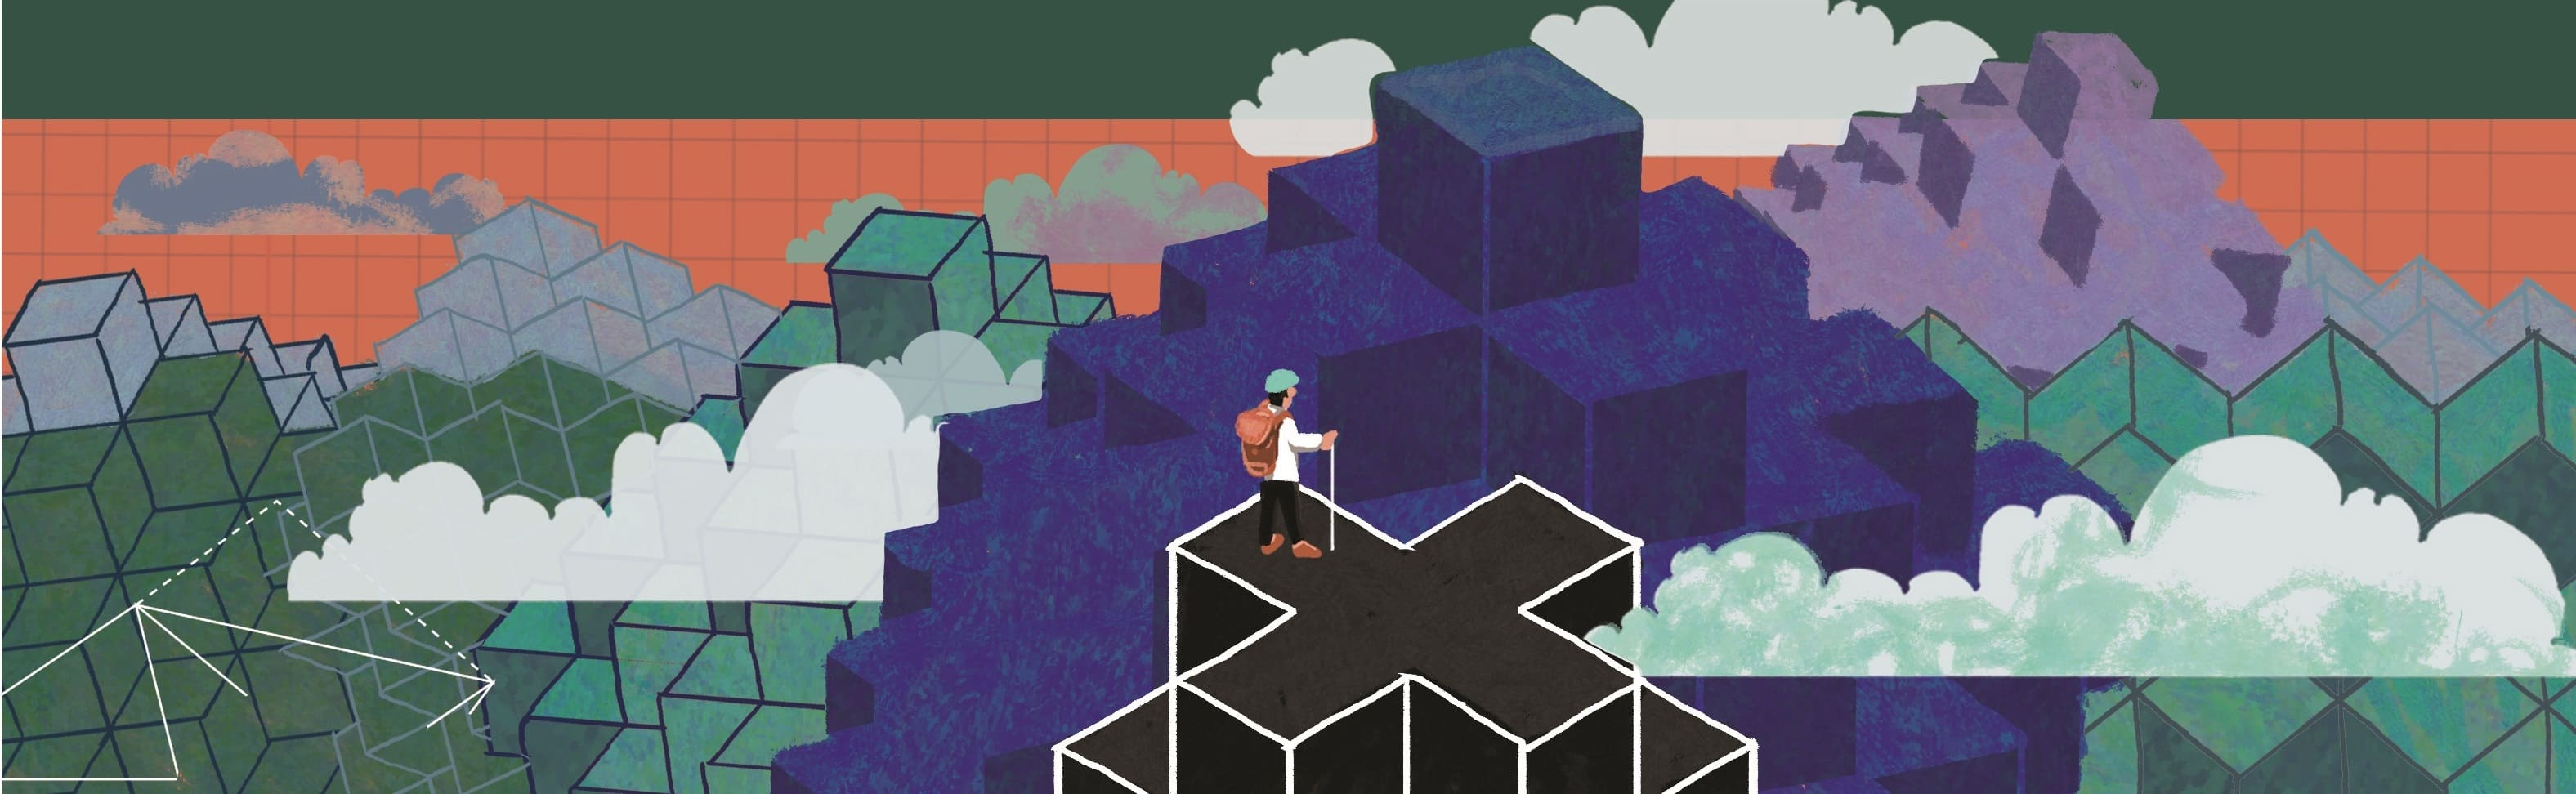
\includegraphics[width=19.3cm]{../thachthuctoanhoc/bannerthachthuc}}}
\centering
\vspace*{4cm}
\endgroup
\vspace*{-8pt}
\begin{tBox}
	\begin{itemize}[leftmargin = 13pt, itemsep = 1.0pt] 
		\item Mỗi bài toán đề xuất (kèm theo lời giải) cần được nêu rõ là bài sáng tác hay bài sưu tầm.
		%		\item Mỗi bài toán đề xuất (kèm theo lời giải) cần được nêu rõ là bài sáng tác hay bài sưu tầm (nếu là bài sưu tầm, cần ghi rõ nguồn).
		\item Bài giải cho mỗi bài toán cần được trình bày trong một file riêng hoặc
		một tờ giấy riêng.
		\item  Người đề xuất bài toán hoặc gửi bài giải cho các bài toán trong mục ``Thách thức kỳ này" cần ghi rõ họ, đệm, tên và nơi làm việc/học tập, số điện thoại liên hệ. Nếu là học sinh (hoặc sinh viên) cần ghi rõ là học sinh lớp mấy (hoặc sinh viên năm thứ mấy).
		\item Các bài toán trong mục Thách thức kỳ này hướng tới các độc giả là học sinh phổ thông; được phân chia thành các mức độ $B$, $A$, và được sắp xếp theo độ khó tăng dần, theo đánh giá chủ quan của Ban biên tập. Các bài toán mức độ $B$ không đòi hỏi các kiến thức vượt quá chương trình môn Toán cấp THCS; các bài toán mức độ $A$ không đòi hỏi các kiến thức vượt quá chương trình môn Toán cấp THPT.
		\item Cách thức gửi bài toán đề xuất hoặc lời giải: gửi file thu được bằng cách scan, ảnh chụp (rõ nét) của bản viết tay, hoặc được soạn thảo bằng các phần mềm Latex, Word tới \url{bbt@pi.edu.vn} hoặc gửi qua đường bưu điện tới Tòa soạn (xem địa chỉ tại bìa $2$).
		\item Hạn gửi lời giải cho các bài toán P$761$--P$770$: trước ngày $15/1/2024$.
	\end{itemize}
\end{tBox}
\begin{center}
	\vspace*{-5pt}
	\textbf{\color{thachthuctoanhoc}\color{thachthuctoanhoc}\color{thachthuctoanhoc}\color{thachthuctoanhoc}\color{thachthuctoanhoc}THÁCH THỨC KỲ NÀY}
	\vspace*{-5pt}
\end{center}
\begin{multicols}{2}
	\setlength{\abovedisplayskip}{4pt}
	\setlength{\belowdisplayskip}{4pt}
	{\color{thachthuctoanhoc}{\usefont{T5}{qag}{b}{n} P761.}}
	(Mức $B$) Mỗi  bạn An, Bình, Huệ, Nga đều có một món tiền tiết kiệm. Biết rằng tổng số tiền tiết kiệm của hai bạn bất kì trong $4$ bạn đó là $1900, 2070, 2110, 2330, 2500$ và $x$ nghìn đồng. Tìm $x$.
	\begin{flushright}
		\textit{Hoàng Việt Vương, Hà Nội}
	\end{flushright}
	{\color{thachthuctoanhoc}{\usefont{T5}{qag}{b}{n} P762.}}
	(Mức $B$) Cho đa giác đều có $2024$ đỉnh, tại mỗi đỉnh ta viết một số nguyên dương không vượt quá $1011$ (mỗi đỉnh viết một số). Chứng minh rằng tồn tại $4$ đỉnh $A,B,C,D$ của đa giác sao cho $ABCD$ là hình chữ nhật, và  $a+b=c+d$, trong đó $a,b,c,d$ tương ứng là các số lần lượt được viết tại các đỉnh $A,B,C,D$. 
	\begin{flushright}
		\textit{Nguyễn Đức Tấn, Tp. Hồ Chí Minh (st)}
	\end{flushright}
	{\color{thachthuctoanhoc}{\usefont{T5}{qag}{b}{n} P762.}}
	(Mức $B$) Cho tam giác $A B C$ có trọng tâm $G$. Dựng ra phía ngoài tam giác đó các tam giác $ABM$ và $ACN$ sao cho $\angle B A M=45^{\circ}$, $A B=3\sqrt2 A M$,  $\angle N A C=90^{\circ}$ và $A C=3 A N$. Chứng minh rằng $\angle G M N=90^{\circ}$.
	\begin{figure}[H]
		\vspace*{-10pt}
		\centering
		\captionsetup{labelformat= empty, justification=centering}
		\definecolor{qqzzcc}{rgb}{0,0.6,0.8}
		\definecolor{qqqqff}{rgb}{0,0,1}
		\definecolor{qqqqffa}{rgb}{1,1,1}
		\definecolor{cqcqcq}{rgb}{0.7529411764705882,0.7529411764705882,0.7529411764705882}
		\begin{tikzpicture}[thachthuctoanhoc,scale=0.58]
			\draw (-1.790333665478168,4.460157886210201) -- (-1.6004915516883682,4.669824220732033) -- (-1.8101578862102001,4.859666334521832) -- (-2,4.65) -- cycle; 
			\draw [shift={(-2,4.65)}] (0,0) -- (-151.55958953937227:0.7) arc (-151.55958953937227:-106.55958953937227:0.7) -- cycle;
			\draw [color=qqzzcc] (-2,4.65)-- (-3.68,-1);
			\draw [color=qqzzcc] (-3.68,-1)-- (4.24,-1);
			\draw [color=qqzzcc] (4.24,-1)-- (-2,4.65);
			\draw  (-3.2216666666666667,3.9883333333333337)-- (-3.68,-1);
			\draw  (-3.2216666666666667,3.9883333333333337)-- (-2,4.65);
			\draw  (-2,4.65)-- (-0.11666666666666714,6.73);
			\draw  (-0.11666666666666714,6.73)-- (4.24,-1);
			\draw  (-3.2216666666666667,3.9883333333333337)-- (-0.48,0.8833333333333334);
			\draw  (-0.48,0.8833333333333334)-- (-0.11666666666666714,6.73);
			\draw  (-0.11666666666666714,6.73)-- (-3.2216666666666667,3.9883333333333337);
			\draw (-2.65,4.55) node[anchor=north west] {\tiny$45^\circ$};
			\draw [fill = white] (-2,4.65) circle (1.5pt);
			\draw[color=qqqqff] (-2.12,5.08) node {$A$};
			\draw [fill = white] (-3.68,-1) circle (1.5pt);
			\draw[color=qqqqff] (-3.92,-1.36) node {$B$};
			\draw [fill = white] (4.24,-1) circle (1.5pt);
			\draw[color=qqqqff] (4.18,-1.36) node {$C$};
			\draw [fill = white] (-3.2216666666666667,3.9883333333333337) circle (1.5pt);
			\draw[color=qqqqff] (-3.54,4.34) node {$M$};
			\draw [fill = white] (-0.11666666666666714,6.73) circle (1.5pt);
			\draw[color=qqqqff] (0.04,7.04) node {$N$};
			\draw [fill = white] (-0.48,0.8833333333333334) circle (1.5pt);
			\draw[color=qqqqff] (-0.52,0.44) node {$G$};
		\end{tikzpicture}
		\vspace*{-15pt}
	\end{figure}
	\begin{flushright}
		\textit{Trần Việt Anh, Nam Định}
	\end{flushright}
	{\color{thachthuctoanhoc}{\usefont{T5}{qag}{b}{n} P764.}}
	(Mức $B$) Tìm tất cả các bộ ba số thực $(x,y,z)$, với $x,y,z\in\left(0,\frac12\right)$ và  thoả mãn 
	\begin{align*}
		\begin{cases}
			\left(3x^2+y^2\right)\sqrt{1-4z^2}\ge z&\\
			\left(3y^2+z^2\right)\sqrt{1-4x^2}\ge x&\\
			\left(3z^2+x^2\right)\sqrt{1-4y^2}\ge y.
		\end{cases}
	\end{align*}
	\begin{flushright}
		\textit{Ngô Văn Trang, Bắc Ninh}
	\end{flushright}
	{\color{thachthuctoanhoc}{\usefont{T5}{qag}{b}{n} P765.}}
	(Mức $B$) Cho số nguyên dương $n$. Gọi $A$ là tích tất cả các số nguyên dương không vượt quá $2n+1$, $B$ là tích tất cả các số nguyên dương lẻ không vượt quá $2n+1$ và $C$ là tích tất cả các số nguyên dương chẵn không vượt quá $2n$. Chứng minh rằng $4A+(B-C-1)^2$ không phải là số chính phương.
	\begin{flushright}
		\textit{Hà Duy Hưng, Hà Nội}
	\end{flushright}
	{\color{thachthuctoanhoc}{\usefont{T5}{qag}{b}{n} P766.}}
	(Mức $B$) Cho $a,b,c$ là các số dương. Chứng minh rằng
	\begin{align*}
		&\dfrac{a^2}{a^2+3ab+2b^2}+\dfrac{b^2}{b^2+3bc+2c^2}\\
		&+\dfrac{c^2}{c^2+3ca+2a^2}\ge \dfrac12.
	\end{align*}
	\begin{flushright}
		\textit{Ngô Văn Thái, Thái Bình}
	\end{flushright}
	{\color{thachthuctoanhoc}{\usefont{T5}{qag}{b}{n} P767.}}
	(Mức $A$) Cho $x,y,z$ là các số thực không âm thoả mãn $x^2+y^2+z^2=3$. Chứng minh rằng
	\begin{align*}
		&3(x+y+x+xyz)\\
		\ge\, &4\sqrt{(x^2+yz)(y^2+zx)(z^2+xy)}.
	\end{align*}
	\begin{flushright}
		\textit{Hoàng Ngọc Minh, Hà Nội}
	\end{flushright}
	{\color{thachthuctoanhoc}{\usefont{T5}{qag}{b}{n} P768.}}
	(Mức $A$) Cho $a$ là một số nguyên dương lẻ và không phải là số chính phương. Chứng minh rằng
	\begin{align*}
		\left[m(a+\sqrt a)\right]\ne \left[n(a-\sqrt a)\right]
	\end{align*}
	với mọi số nguyên dương $m,n$. 
	\begin{flushright}
		\textit{Nguyễn Hoàng Duy, Thái Bình (st)}
	\end{flushright}
	\vskip 0.1cm
	\columnbreak
	{\color{thachthuctoanhoc}{\usefont{T5}{qag}{b}{n} P769.}}
	(Mức $A$) Cho tam giác không cân $ABC$ nội tiếp đường tròn $(O)$. $K$ là một điểm (khác $A$) trên tiếp tuyến tại $A$ của $(O)$. $\Delta$ là một đường thẳng đi qua $K$, cắt $BC, CA, AB$ lần lượt tại $D, E, F$. Chứng minh rằng tâm đẳng phương của các đường tròn: đường tròn đường kính $EF$, đường tròn đường kính $DK$, đường tròn $(O)$ thuộc đường thẳng $\Delta.$
	\begin{center}
		\definecolor{qqqqff}{rgb}{0,0,1}
		\definecolor{qqqqffa}{rgb}{1,1,1}
		\definecolor{cqcqcq}{rgb}{0.7529411764705882,0.7529411764705882,0.7529411764705882}
		\begin{tikzpicture}[thachthuctoanhoc, scale=0.54]
			\draw  (-4.38,5.01)-- (-5.56,-0.3);
			\draw  (-5.56,-0.3)-- (1.58,-0.3);
			\draw  (1.58,-0.3)-- (-4.38,5.01);
			\draw  (-1.99,1.6927777777777777) circle (4.08852825251397cm);
			\draw  (-7.256570958905223,2.93748144947073)-- (5.1899690781026155,-0.3);
			\draw  (1.58,-0.3)-- (5.1899690781026155,-0.3);
			\draw  (-7.256570958905223,2.93748144947073)-- (-4.38,5.01);
			\draw [fill = white] (-4.38,5.01) circle (1.5pt);
			\draw[color=qqqqff] (-4.44,5.5) node {$A$};
			\draw [fill = white] (-5.56,-0.3) circle (1.5pt);
			\draw[color=qqqqff] (-5.94,-0.5) node {$B$};
			\draw [fill = white] (1.58,-0.3) circle (1.5pt);
			\draw[color=qqqqff] (1.7,-0.73) node {$C$};
			\draw [fill = white] (-7.256570958905223,2.93748144947073) circle (1.5pt);
			\draw[color=qqqqff] (-7.72,3.06) node {$K$};
			\draw [fill = white] (5.1899690781026155,-0.3) circle (1.5pt);
			\draw[color=qqqqff] (5.14,-0.73) node {$D$};
			\draw [fill = white] (0.09149352555368925,1.0261693589446155) circle (1.5pt);
			\draw[color=qqqqff] (0.2,1.52) node {$E$};
			\draw [fill = white] (-4.972579921493512,2.343390353279194) circle (1.5pt);
			\draw[color=qqqqff] (-5.22,2.8) node {$F$};
		\end{tikzpicture}
	\end{center}
	\begin{flushright}
		\textit{Lưu Công Đông, Hà Nội}
	\end{flushright}
	{\color{thachthuctoanhoc}{\usefont{T5}{qag}{b}{n} P770.}}
	(Mức $A$) Cho phép thực hiện việc đổi chỗ các số hạng trong một hoán vị, theo qui tắc: Mỗi lần, lấy ra khỏi hoán vị tám số hạng tùy ý của nó, rồi lại xếp tám số hạng đó vào tám vị trí mà chúng đã nằm, nhưng theo thứ tự ngược lại.
	Hỏi, nhờ việc thực hiện liên tiếp một số hữu hạn lần phép đổi chỗ nói trên đối với hoán vị $(1,2,\ldots,2023)$ của $2023$ số nguyên dương đầu tiên, ta có thể nhận được hoán vị $(2023,2022,\ldots,1)$ hay không?
	\begin{flushright}
		\textit{Nguyễn Khắc Minh, Hà Nội}
	\end{flushright}
\end{multicols}
\newpage
\centerline{{\large{\textbf{\color{thachthuctoanhoc}\color{thachthuctoanhoc}\color{thachthuctoanhoc}GIẢI BÀI KỲ TRƯỚC}}}}
\vspace*{-5pt}
\begin{multicols}{2}
	\setlength{\abovedisplayskip}{5pt}
	\setlength{\belowdisplayskip}{5pt}
	{\color{thachthuctoanhoc}{\usefont{T5}{qag}{b}{n} P731.}}
	(Mức $B$) Ghép chín hình vuông thành một hình chữ nhật, như ở hình dưới đây. Biết rằng, hình vuông màu đen có cạnh bằng $1$. Tìm chiều dài và chiều rộng của hình chữ nhật.
	\begin{figure}[H]
		\vspace*{-5pt}
		\centering
		\captionsetup{labelformat= empty, justification=centering}
		\begin{tikzpicture}[thachthuctoanhoc,scale=0.15]
			\draw[fill=black] (0,0) rectangle (1,1);
			\draw  (0.,-9.)-- (9.,-9.);
			\draw  (9.,-9.)-- (9.,0.);
			\draw  (9.,0.)-- (0.,0.);
			\draw  (0.,0.)-- (0.,-9.);
			\draw  (1.,0.)-- (9.,0.);
			\draw  (9.,0.)-- (9.,8.);
			\draw  (9.,8.)-- (1.,8.);
			\draw  (1.,8.)-- (1.,0.);
			\draw  (-10.,-9.)-- (0.,-9.);
			\draw  (0.,-9.)-- (0.,1.);
			\draw  (0.,1.)-- (-10.,1.);
			\draw  (-10.,1.)-- (-10.,-9.);
			\draw  (-6.,1.)-- (1.,1.);
			\draw  (1.,1.)-- (1.,8.);
			\draw  (1.,8.)-- (-6.,8.);
			\draw  (-6.,8.)-- (-6.,1.);
			\draw  (-10.,1.)-- (-6.,1.);
			\draw  (-6.,1.)-- (-6.,5.);
			\draw  (-6.,5.)-- (-10.,5.);
			\draw  (-10.,5.)-- (-10.,1.);
			\draw  (-6.,8.)-- (9.,8.);
			\draw  (9.,8.)-- (9.,23.);
			\draw  (9.,23.)-- (-6.,23.);
			\draw  (-6.,23.)-- (-6.,8.);
			\draw  (-24.,-9.)-- (-10.,-9.);
			\draw  (-10.,-9.)-- (-10.,5.);
			\draw  (-10.,5.)-- (-24.,5.);
			\draw  (-24.,5.)-- (-24.,-9.);
			\draw  (-24.,5.)-- (-6.,5.);
			\draw  (-6.,5.)-- (-6.,23.);
			\draw  (-6.,23.)-- (-24.,23.);
			\draw  (-24.,23.)-- (-24.,5.);	
		\end{tikzpicture}
		\vspace*{-10pt}
	\end{figure} 
	\textbf{\color{thachthuctoanhoc}Lời giải} \textit{(dựa theo tất cả lời giải Tạp chí đã nhận được từ bạn đọc})\textbf{\color{thachthuctoanhoc}.}
	\vskip 0.05cm
	Đặt tên các hình vuông như ở hình vẽ dưới đây:
	\begin{figure}[H]
		\vspace*{-5pt}
		\centering
		\captionsetup{labelformat= empty, justification=centering}
		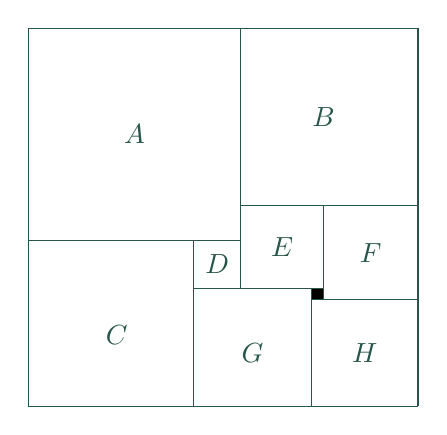
\begin{tikzpicture}[thachthuctoanhoc,scale=0.15]
			\draw[fill=black] (0,0) rectangle (1,1);
			\draw  (0.,-9.)-- (9.,-9.);
			\draw  (9.,-9.)-- (9.,0.);
			\draw (4.5,-4.5) node {$H$};
			\draw (5,4) node {$F$};
			\draw (-2.5,4.5) node {$E$};
			\draw (-5,-4.5) node {$G$};
			\draw (-8,3) node {$D$};
			\draw (1,15.5) node {$B$};
			\draw (-15,14) node {$A$};
			\draw (-16.5,-3) node {$C$};
			\draw  (9.,0.)-- (0.,0.);
			\draw  (0.,0.)-- (0.,-9.);
			\draw  (1.,0.)-- (9.,0.);
			\draw  (9.,0.)-- (9.,8.);
			\draw  (9.,8.)-- (1.,8.);
			\draw  (1.,8.)-- (1.,0.);
			\draw  (-10.,-9.)-- (0.,-9.);
			\draw  (0.,-9.)-- (0.,1.);
			\draw  (0.,1.)-- (-10.,1.);
			\draw  (-10.,1.)-- (-10.,-9.);
			\draw  (-6.,1.)-- (1.,1.);
			\draw  (1.,1.)-- (1.,8.);
			\draw  (1.,8.)-- (-6.,8.);
			\draw  (-6.,8.)-- (-6.,1.);
			\draw  (-10.,1.)-- (-6.,1.);
			\draw  (-6.,1.)-- (-6.,5.);
			\draw  (-6.,5.)-- (-10.,5.);
			\draw  (-10.,5.)-- (-10.,1.);
			\draw  (-6.,8.)-- (9.,8.);
			\draw  (9.,8.)-- (9.,23.);
			\draw  (9.,23.)-- (-6.,23.);
			\draw  (-6.,23.)-- (-6.,8.);
			\draw  (-24.,-9.)-- (-10.,-9.);
			\draw  (-10.,-9.)-- (-10.,5.);
			\draw  (-10.,5.)-- (-24.,5.);
			\draw  (-24.,5.)-- (-24.,-9.);
			\draw  (-24.,5.)-- (-6.,5.);
			\draw  (-6.,5.)-- (-6.,23.);
			\draw  (-6.,23.)-- (-24.,23.);
			\draw  (-24.,23.)-- (-24.,5.);	
		\end{tikzpicture}
		\vspace*{-10pt}
	\end{figure} 
	Gọi $a, b, c, d, e, g, h$ tương ứng là độ dài cạnh của các hình vuông $A, B, C, D, E, G, H$.
	\vskip 0.1cm
	Gọi $x$ là độ dài cạnh của hình vuông $F$.
	\vskip 0.1cm
	Khi đó, do hình vuông màu đen có cạnh bằng $1$, nên
	\begin{align*}
		&e = x - 1; b = e + x = 2x - 1;\\
		&h = x + 1; g = h + 1 = x + 2;\\
		&d = g - (e - 1) = (x + 2) - (x - 2) = 4;\\
		&c = g + d = (x + 2) + 4 = x + 6;\\
		&a = c + d = (x + 6) + 4 = x + 10.
	\end{align*}
	Từ đó, do $a + c = b + x + h$, nên ta có:
	\begin{align*}
		(x + 10) + (x + 6) = (2x - 1) + x + (x + 1).
	\end{align*}
	Suy ra, $2x + 16 = 4x$. Do đó, $x = 8$. Suy ra
	\begin{align*}
		&a = 8 + 10 = 18, b = 2\cdot8 - 1 = 15 \\
		\text{ và } &c = 8 + 6 = 14.
	\end{align*}
	Vì vậy, hình chữ nhật có chiều dài là:
	\begin{align*}
		18 + 15 = 33,
	\end{align*}
	và chiều rộng là: $18 + 14 = 32$.
	\vskip 0.05cm
	\textbf{\color{thachthuctoanhoc}Bình luận và Nhận xét}
	\vskip 0.05cm	
	Tất cả lời giải Tạp chí đã nhận được từ bạn đọc đều là lời giải đúng và hoàn chỉnh.
	\begin{flushright}
		\textbf{\color{thachthuctoanhoc}Hà Thanh}
	\end{flushright}
	{\color{thachthuctoanhoc}{\usefont{T5}{qag}{b}{n} P732.}}
	(Mức $B$) Xét bốn số thực (không nhất thiết đôi một khác nhau), mà mỗi số có trị tuyệt đối không vượt quá $\dfrac{1}{2}$, và tổng của ba số bất kỳ, trong bốn số đó, là một số nguyên. Tìm tất cả các giá trị có thể của tổng bốn số đó.
	\vskip 0.05cm
	\textbf{\color{thachthuctoanhoc}Lời giải} (\textit{phỏng theo cách giải của bạn Ngô Minh Chấn, lớp $9$A$3$, trường TH$\&$THCS Archimedes Đông Anh, Tp. Hà Nội})\textbf{\color{thachthuctoanhoc}.}
	\vskip 0.05cm
	Gọi $a, b, c, d$ là bốn số thực thỏa mãn các điều kiện đã nêu trong đề bài.
	\vskip 0.05cm
	Đặt $x = a \!+\! b \!+\! c$, $y = a \!+\! b \!+\! d$, $z = a \!+\! c \!+\! d$, $t = b + c + d$, và
	$s = a + b + c + d$.
	\vskip 0.05cm
	Khi đó, theo giả thiết của bài ra, ta có:
	\begin{align*}
		|a| \le \frac{1}{2}, |b| \le \frac{1}{2},|c| \le \frac{1}{2},|d| \le \frac{1}{2}; \tag{$1$}
	\end{align*}
	và $x, y, z, t$ là các số nguyên.        \hfill ($2$)
	\vskip 0.05cm
	Xét cặp số $x, y$.
	Do ($2$) nên $x - y$ là một số nguyên; hơn nữa
	\begin{align*}
		\left| {x - y} \right| &= \left| {c - d} \right| \le |c| + \left| {d} \right| \\
		&\le 1 \quad\text{(do ($1$))}. \tag{$3$}
	\end{align*}
	Vì thế, $\left| {x - y} \right| \in \left\{ {0;1} \right\}.$ \hfill ($4$)
	\vskip 0.05cm
	Nếu $|x - y| = 1$  thì theo ($3$), phải có:
	\begin{align*}
		\left| {c - d} \right| = |c| + \left| {d} \right| = 1.
	\end{align*}
	Điều vừa nêu trên tương đương với
	\begin{align*}
	\quad\quad	\begin{cases}
			cd \le 0\\
			|c| = |d| = \dfrac{1}{2} \text{ (do ($1$)).} \quad\quad\quad\quad \text{($5$)} 
		\end{cases}
	\end{align*}
	Suy ra, $c + d = 0$. Do đó, $z = a$ và $t = b$. Vì thế, $a,b \in \mathbb{Z}$  (do ($2$)). Từ đây và ($1$), suy ra $a = b = 0$.
	\vskip 0.05cm
	Vì vậy, $x = c$. Do đó,  $c \in \mathbb{Z}$. Từ đây và ($1$), suy ra $c = 0$, mâu thuẫn với ($5$).
	\vskip 0.05cm
	Mâu thuẫn nhận được ở trên cho thấy
	\begin{align*}
		|x - y| \ne 1.
	\end{align*}
	Do đó, từ ($4$) ta được $x = y$.
	\vskip 0.05cm
	Xét các cặp số $x, z$ và $x, t$, bằng cách hoàn toàn tương tự, ta sẽ được $x = z$ và $x = t$.
	\vskip 0.05cm
	Vì vậy, $x = y = z = t$. Suy ra
	\begin{align*}
		3s = x  + y + z + t = 4x;
	\end{align*}
	do đó, $s = \dfrac{4}{3}x$. \hfill ($6$)
	\vskip 0.05cm
	Tiếp theo, ta có:
	\begin{align*}
		|x| \le |a| + |b| + |c| \le \frac{3}{2} \quad\text{(do ($1$))}; 
	\end{align*}
	mà $|x| \in \mathbb{Z}$  (theo ($2$)), nên  $|x| \in \{0;1\}$. \hfill ($7$)
	\vskip 0.05cm
	Từ ($6$) và ($7$), suy ra $s \in \{-\dfrac{4}{3}; 0; \dfrac{4}{3}\}$.
	\vskip 0.05cm 
	Ngược lại, dễ thấy:
	\vskip 0.05cm
	$\bullet$ $a=b=c=d = -\dfrac{1}{3}$   là bốn số thực thỏa mãn các điều kiện của đề bài, và có tổng bằng $- \dfrac{4}{3}$;
	\vskip 0.05cm  
	$\bullet$  $a=b=c=d = 0$  là bốn số thực thỏa mãn các điều kiện của đề bài, và có tổng bằng $0$;
	\vskip 0.05cm
	$\bullet$ $a=b=c=d = \dfrac{1}{3}$   là bốn số thực thỏa mãn các điều kiện của đề bài, và có tổng bằng $\dfrac{4}{3}$;
	\vskip 0.05cm  
	Vậy, tất cả các giá trị có thể của tổng bốn số thỏa mãn các điều kiện của đề bài là:  $- \dfrac{4}{3}, 0, \dfrac{4}{3}$.
	\vskip 0.05cm  
	\textbf{\color{thachthuctoanhoc}Bình luận và Nhận xét}
	\vskip 0.05cm
	$\pmb{1.}$ Lời giải trên cho thấy, các bộ bốn số thực được liệt kê ở phần cuối của Lời giải là \textit{tất cả} các bộ bốn số thực thỏa mãn các điều kiện của đề bài.
	\vskip 0.05cm
	$\pmb{2.}$ Trong số các lời giải Tạp chí đã nhận được từ bạn đọc, rất tiếc, có hai lời giải sai, do người giải bài hoặc mới chỉ ra điều kiện cần (nhưng không đủ) cho giá trị của tổng bốn số đã vội kết luận đó là các giá trị có thể của tổng đó, hoặc đã chỉ ra sai các bộ bốn số thực thỏa mãn các điều kiện của đề bài. Bên cạnh đó, còn có một lời giải chưa đầy đủ, do người giải bài chưa xét hết các trường hợp có thể xảy~ra.
	\begin{flushright}
		\textbf{\color{thachthuctoanhoc}Hà Thanh}
	\end{flushright}
	{\color{thachthuctoanhoc}{\usefont{T5}{qag}{b}{n} P733.}}
	(Mức $B$)
	Tìm giá trị nhỏ nhất của biểu thức
	\begin{align*}
		S = \left\lfloor {\frac{{b + c}}{a}} \right\rfloor  + \left\lfloor {\frac{{c + a}}{b}} \right\rfloor  + \left\lfloor {\frac{{a + b}}{c}} \right\rfloor ,
	\end{align*}
	trong đó, $a, b, c$ là các biến nguyên dương.
	($\left\lfloor x \right\rfloor $  ký hiệu số nguyên lớn nhất không vượt quá $x$.)
	\vskip 0.05cm
	\textbf{\color{thachthuctoanhoc}Lời giải} (\textit{dựa theo lời giải của các bạn: Ngô Minh Chấn, lớp $9$A$3$, trường TH$\&$THCS Archimedes Đông Anh, Tp. Hà Nội; Lê Nguyễn Hoàng Nhật Đình, lớp $9$C, trường THCS Nguyễn Thái Bình, tỉnh Cà Mau; Trương Anh Dũng, lớp $10$A$1$ chuyên Toán, trường THPT chuyên Vĩnh Phúc, tỉnh Vĩnh Phúc})\textbf{\color{thachthuctoanhoc}.}
	\vskip 0.05cm
	Từ định nghĩa phần nguyên của một số thực dễ thấy, với mọi số thực $x$, ta đều có
	\begin{align*}
		\left\lfloor x \right\rfloor  > x -1.
	\end{align*}
	Vì vậy, với lưu ý $a, b, c$ là các số dương, ta có:
	\begin{align*}
			S &> \frac{{b + c}}{a} + \frac{{c + a}}{b} + \frac{{a + b}}{c} - 3 \\
			&= \left( {\frac{b}{a} + \frac{a}{b}} \right) + \left( {\frac{c}{a} + \frac{a}{c}} \right) + \left( {\frac{c}{b} + \frac{b}{c}} \right) - 3\\
			 &\ge 2\sqrt {\frac{b}{a} \!\cdot\! \frac{a}{b}}  \!+\! 2\sqrt {\frac{c}{a} \!\cdot\! \frac{a}{c}}  \!+\! 2\sqrt {\frac{c}{b} \!\cdot\! \frac{b}{c}}  \!-\! 3 \!=\! 3.
	\end{align*}
	Từ đó, do $S$ là số nguyên, suy ra $S \ge 4$.
	\vskip 0.05cm
	Hơn nữa, dễ thấy, với $a = 3, b = c = 4$, ta có $S = 4$.
	\vskip 0.05cm
	Vì vậy, giá trị nhỏ nhất của $S$ bằng $4$.
	\vskip 0.05cm
	\textbf{\color{thachthuctoanhoc}Bình luận và Nhận xét}
	\vskip 0.05cm
	$\pmb{1.}$ Lời giải trên cho thấy, kết quả của bài ra không thay đổi, khi thay giả thiết ``$a, b, c$ là các biến nguyên dương" bởi giả thiết ``$a, b, c$ là các biến thực dương".
	\vskip 0.05cm
	$\pmb{2.}$ Trong số các lời giải Tạp chí đã nhận được từ bạn đọc, rất tiếc, có một lời giải sai, do người giải bài đã mắc sai sót về kiến thức cơ bản, khi khẳng định ``$\left\lfloor x \right\rfloor  \ge x$  với mọi số thực $x$".
	\begin{flushright}
		\textbf{\color{thachthuctoanhoc}Lưu Thị Thanh Hà}
	\end{flushright}
	{\color{thachthuctoanhoc}{\usefont{T5}{qag}{b}{n} P734.}}
	(Mức $B$) Cho hình vuông $ABCD$. Gọi $E$ là trung điểm của $AD$; $H$ là hình chiếu vuông góc của $B$ trên $CE$. Trên đường chéo $AC$, lấy điểm $M$ sao cho $AM = \dfrac{3}{8}AC$. Chứng minh rằng, $ME$ song song với $DH$.
	\vskip 0.05cm
	\textbf{\color{thachthuctoanhoc}Lời giải} (\textit{dựa theo lời giải của bạn Nguyễn Nguyên Chinh, lớp $9$D, trường THCS Nguyễn Chí Thanh, tỉnh Phú Yên})\textbf{\color{thachthuctoanhoc}.}
	\begin{figure}[H]
		\vspace*{-5pt}
		\centering
		\captionsetup{labelformat= empty, justification=centering}
		\definecolor{qqwuqq}{rgb}{0.,0.39215686274509803,0.}
		\definecolor{uuuuuu}{rgb}{0.26666666666666666,0.26666666666666666,0.26666666666666666}
		\definecolor{qqqqff}{rgb}{0.,0.,1.}
		\begin{tikzpicture}[thachthuctoanhoc,scale=0.45]
			\draw [shift={(10.,5.)},pattern color=qqwuqq,fill=qqwuqq,fill opacity=0.10000000149011612] (0,0) -- (-116.56505117707799:0.8153190950798923) arc (-116.56505117707799:-90.:0.8153190950798923) -- cycle;
			\draw [shift={(10.,-4.)},pattern color=qqwuqq,fill=qqwuqq,fill opacity=0.10000000149011612] (0,0) -- (153.43494882292202:0.8153190950798923) arc (153.43494882292202:180.:0.8153190950798923) -- cycle;
			\draw[pattern color=qqwuqq,fill=qqwuqq,fill opacity=0.10000000149011612] (6.743768714703979,-2.3718843573519894) -- (6.915653072055969,-2.028115642648011) -- (6.57188435735199,-1.8562312852960212) -- (6.4,-2.2) -- cycle; 
			\draw[pattern color=qqwuqq,fill=qqwuqq,fill opacity=0.10000000149011612] (1.3843451073079143,-4.) -- (1.3843451073079143,-3.6156548926920857) -- (1.,-3.6156548926920857) -- (1.,-4.) -- cycle; 
			\draw  (1.,5.)-- (10.,5.);
			\draw  (1.,-4.)-- (10.,-4.);
			\draw  (10.,-4.)-- (10.,5.);
			\draw  (1.,5.)-- (10.,-4.);
			\draw [color=qqqqff] (1.,0.5)-- (4.375,1.625);
			\draw  (1.,0.5)-- (10.,-4.);
			\draw [color=qqqqff] (6.4,-2.2)-- (1.,-4.);
			\draw  (6.4,-2.2)-- (10.,5.);
			\draw  (1.,-7.)-- (1.,-4.);
			\draw [color=qqqqff] (1.,-7.)-- (10.,-4.);
			\draw (-0.44481130622791615,6.007702325581402) node[anchor=north west] {$A$};
			\draw (10.011222021831985,6.134879628750732) node[anchor=north west] {$B$};
			\draw (10.038399325001315,-3.477176480514691) node[anchor=north west] {$C$};
			\draw (-0.2002155777039485,-3.341289964668042) node[anchor=north west] {$D$};
			\draw (-0.2002155777039485,1.1157877551020416) node[anchor=north west] {$E$};
			\draw (5.934626546432524,-2.20639567157095424) node[anchor=north west] {$H$};
			\draw (4.30398835627274,2.55618482307652) node[anchor=north west] {$M$};
			\draw (0.44481130622791615,-6.92807467172924) node[anchor=north west] {$N$};
			\draw  (1.,0.5)-- (1.,5.);
			\draw  (0.8777021357380159,2.7024397194536727) -- (1.1222978642619836,2.7024397194536727);
			\draw  (0.8777021357380159,2.797560280546327) -- (1.1222978642619836,2.797560280546327);
			\draw  (1.,0.5)-- (1.,-4.);
			\draw  (1.1222978642619836,-1.7024397194536725) -- (0.8777021357380159,-1.7024397194536725);
			\draw  (1.1222978642619836,-1.7975602805463267) -- (0.8777021357380159,-1.7975602805463267);
				\draw [fill=qqqqff] (1.,5.) circle (1.5pt);
				\draw [fill=qqqqff] (10.,5.) circle (1.5pt);
				\draw [fill=qqqqff] (10.,-4.) circle (1.5pt);
				\draw [fill=qqqqff] (1.,-4.) circle (1.5pt);
				\draw [fill=uuuuuu] (1.,0.5) circle (1.5pt);
				\draw [fill=qqqqff] (4.375,1.625) circle (1.5pt);
				\draw [fill=uuuuuu] (6.4,-2.2) circle (1.5pt);
				\draw [fill=uuuuuu] (1.,-7.) circle (1.5pt);
		\end{tikzpicture}
		\vspace*{-10pt}
	\end{figure}
	Qua $C$, kẻ đường thẳng song song với $ME$, cắt đường thẳng $AD$ tại $N$.
	\vskip 0.05cm
	Khi đó, theo định lý Thales, ta có:
	\begin{align*}
		\frac{{AN}}{{AE}} = \frac{{AC}}{{AM}} = \frac{8}{3} \quad\text{(theo giả thiết).}
	\end{align*}
	Từ đó, với lưu ý $E$ là trung điểm của $AD$ (giả thiết), suy ra
	\begin{align*}
		\frac{{DN}}{{DE}} = \frac{{DN}}{{AE}} = \frac{{AN}}{{AE}} - \frac{{AD}}{{AE}} = \frac{8}{3} - 2 = \frac{2}{3}.
	\end{align*}
	Do đó
	\begin{align*}
		\frac{{NE}}{{ND}} &= \frac{{ND + DE}}{{ND}} = 1 + \frac{{DE}}{{ND}} \\
		&= 1 + \frac{3}{2} = \frac{5}{2}. \tag{$1$}
	\end{align*}
	Đặt $AD = a$. Từ giả thiết của bài ra, ta có $CD = a$ và
	\begin{align*}
		AE = \frac{{AD}}{2} = \frac{a}{2}.
	\end{align*}
	Vì vậy, áp dụng định lý Pithagoras cho tam giác vuông $CDE$, ta được:
	\begin{align*}
		C{E^2} &= C{D^2} + D{E^2} \\
		&= {a^2} + {\left( {\frac{a}{2}} \right)^2} = \frac{5}{4}{a^2}. \tag{$2$}
	\end{align*}
	Tiếp theo, do
	\begin{align*}
		\angle CBH = {90^{\rm{o}}} - \angle BCH = \angle DCE,
	\end{align*}
	nên tam giác vuông $BHC$ đồng dạng với tam giác vuông $CDE$. Do đó
	\begin{align*}
		\frac{{CH}}{{CB}} = \frac{{ED}}{{EC}};
	\end{align*}
	suy ra
	\begin{align*}
			\frac{{CH}}{{CE}} = \frac{{ED \cdot CB}}{{C{E^2}}} = \frac{{\dfrac{a}{2} \cdot a}}{{\dfrac{5}{4}{a^2}}}\quad\left( {{\rm{theo}}(2)} \right)\\
			 = \frac{2}{5} = \frac{{ND}}{{NE}}\quad\left( {{\rm{theo}}(1)} \right).
	\end{align*}
	Do đó, $DH \parallel NC$ (theo định lý Thales); mà $NC \parallel ME$, nên $DH \parallel ME$.
	\vskip 0.05cm
	Ta có điều phải chứng minh theo yêu cầu đề bài. 
	\vskip 0.05cm
	\textbf{\color{thachthuctoanhoc}Bình luận và Nhận xét}
	\vskip 0.05cm
	Trong số các lời giải Tạp chí đã nhận được từ bạn đọc, có một lời giải bằng phương pháp tọa độ. Rất tiếc, lời giải này được diễn đạt rất sai bằng ngôn ngữ Toán học; và vì thế, không thể coi là lời giải đúng.
	\begin{flushright}
		\textbf{\color{thachthuctoanhoc}Hạ Vũ Anh}
	\end{flushright}
	{\color{thachthuctoanhoc}{\usefont{T5}{qag}{b}{n} P735.}}
	(Mức $B$) Tìm tất cả các số nguyên dương $n$, để $n! + n$ là một lũy thừa với số mũ nguyên dương của một số nguyên tố.
	\vskip 0.05cm
	\textbf{\color{thachthuctoanhoc}Lời giải} (\textit{dựa theo đa số lời giải Tạp chí đã nhận được từ bạn đọc})\textbf{\color{thachthuctoanhoc}.}
	\vskip 0.05cm
	$\bullet$ Giả sử $n$ là số nguyên dương thỏa mãn yêu cầu đề bài.
	\vskip 0.05cm
	Khi đó, tồn tại số nguyên tố $p$ và số nguyên dương $\alpha$, sao cho
	\begin{align*}
		n! + n = {p^\alpha },
	\end{align*}
	hay  
	\begin{align*}
		n\left( {\left( {n - 1} \right)! + 1} \right) = {p^\alpha }. \tag{$1$}
	\end{align*}
	Do $\left( {n - 1} \right)! + 1 > 1$  nên từ ($1$) suy ra, tồn tại số tự nhiên $\beta < \alpha$, sao cho $n = p^{\beta}$  và
	\begin{align*}
		\left( {n - 1} \right)! + 1 = {p^{\alpha  - \beta }}. \tag{$2$}
	\end{align*}
	Vì  $\beta \in  \mathbb{N}, \alpha \in \mathbb{N^*}$   và $\beta < \alpha$, nên  $\alpha - \beta$ là một số nguyên dương. Do đó, từ ($2$) suy ra
	\begin{align*}
		\left( {n - 1} \right)! + 1 \equiv 0\left( {\bmod p} \right). \tag{$3$}
	\end{align*}
	Từ ($2$) và ($3$) suy ra $\beta \in \{0;1\}$, vì nếu ngược lại, $\beta \ge 2$,  thì
	\begin{align*}
		n - 1 \ge {p^2} - 1 > p \text{ (do $n = p^{\beta}$  và $p \ge 2$)};
	\end{align*}
	dẫn tới $\left( {n - 1} \right)! \,\,\vdots\,\, p,$  và do đó,  $1 \,\,\vdots\,\, p$ (theo ($3$)), là điều vô lý.
	\vskip 0.05cm
	Với $\beta= 0$, ta có $n = p^0 = 1$. \hfill ($4$)
	\vskip 0.05cm
	Với $\beta = 1$, ta có $n = p$; do đó
	\begin{align*}
		\left( {p - 1} \right)! + 1 = {p^{\alpha  - 1}}	\quad\text{(theo ($2$))}. \tag{$5$}
	\end{align*}                                                      
	Xét $p > 5$. Khi đó
	\begin{align*}
		\left( {p - 1} \right)! > \left( {p - 1} \right)\left( {p - 2} \right) > p.
	\end{align*}
	Vì thế, từ ($5$) suy ra $\alpha -1\ge 2$, hay $\alpha \ge 3$. Do vậy, từ ($5$) ta có:
	\begin{align*}
		&\left( {p - 1} \right)! = {p^{\alpha  - 1}} - 1 \\
		=\, &\left( {p - 1} \right)\left( {{p^{\alpha  - 2}} + {p^{\alpha  - 3}} +  \cdots  + p + 1} \right).
	\end{align*}
	Suy ra
	\begin{align*}
		\left( {p \!-\! 2} \right)! \!=\! {p^{\alpha  \!-\! 2}} \!+\! {p^{\alpha  \!-\! 3}} \!+\!  \cdots  \!+\! p \!+\! 1. \tag{$6$}
	\end{align*}
	Tiếp theo, do $p$ là số nguyên tố lớn hơn $5$ nên $p - 1$ là một hợp số lớn hơn $4$. Vì thế, tồn tại các số nguyên dương $a, b$, với $1 < a \le b$, sao cho $p - 1 = ab$.
	\vskip 0.05cm
	-- Nếu $a = b$ thì
	\begin{align*}
		4 < p - 1 = {a^2}. \tag{$7$}
	\end{align*}
	Do đó, $a > 2$; suy ra $p - 1 > 2a$. Vì thế, $p - 2 > 2a - 1$; mà $p - 2$ là số nguyên, nên $p - 2 \ge 2a$. Vì vậy
	\begin{align*}
	\left( {p - 2} \right)! &= 1 \cdot 2 \cdot  \cdots  \cdot a \cdot  \cdots  \cdot 2a \cdot  \cdots  \cdot \left( {p - 2} \right) \\
	&\equiv 0\left(\!\! {\bmod p - 1} \right)	\,\,\,\text{(do ($7$))}.
	\end{align*}
	-- Nếu $a < b$ thì do $a, b < p - 2$ nên
	\begin{align*}
		\left( {p - 2} \right)! &= 1 \cdot 2 \cdot  \cdots  \cdot a \cdot  \cdots  \cdot b \cdot  \cdots  \cdot \left( {p - 2} \right) \\
		&\equiv 0\left(\!\! {\bmod p - 1} \right) \,\,\,\text{(do $p - 1 = ab$).}
	\end{align*}
	Vì vậy, ta có
	\begin{align*}
		\left( {p - 2} \right)! \equiv 0\left( {\bmod p - 1} \right). \tag{$8$}
	\end{align*}
	Do $p \equiv 1\left( {\bmod p - 1} \right)$  nên từ ($6$) suy ra
	\begin{align*}
		\left( {p - 2} \right)! \equiv \alpha  - 1\left( {\bmod p - 1} \right). \tag{$9$}
	\end{align*}
	Từ ($8$) và ($9$), ta được:
	\begin{align*}
		\alpha  - 1 \equiv 0\left( {\bmod p - 1} \right);
	\end{align*}
	mà $\alpha - 1$ là số nguyên dương, nên $\alpha - 1 \ge p - 1$, hay $\alpha \ge p$. Vì thế, theo ($5$), ta có
	\begin{align*}
		\left( {p - 1} \right)! + 1 \ge {p^{p - 1}},
	\end{align*}
	là điều vô lý.
	\vskip 0.05cm
	Điều vô lý vừa nhận được ở trên cho thấy, $p \le 5$; mà $p$ là số nguyên tố, nên \linebreak$p \in \{2; 3; 5\}$. \hfill      ($10$)
	\vskip 0.05cm
	Do $n = p$ nên từ ($4$) và ($10$), ta được: \linebreak$n \in \{1; 2; 3; 5\}$. \hfill ($11$)
	\vskip 0.05cm
	$\bullet$ Ngược lại, với $n$ thỏa mãn ($11$), ta có
	\begin{align*}
		n! + n \in S = \{2; 4; 9; 125\}.
	\end{align*}
	Dễ thấy, mỗi số thuộc $S$ đều là một lũy thừa với số mũ nguyên dương của một số nguyên tố.
	\vskip 0.05cm
	$\bullet$ Vậy, tất cả các số nguyên dương cần tìm theo yêu cầu đề bài là: $1, 2, 3$ và $5$.
	\vskip 0.05cm 
	\textbf{\color{thachthuctoanhoc}Bình luận và Nhận xét}
	\vskip 0.05cm
	$\pmb{1.}$ Dễ thấy, trong Lời giải trên ẩn chứa chứng minh của kết quả sau:
	\vskip 0.05cm
	``\textit{Nếu $n$ là một hợp số lớn hơn $4$ thì}  
	\begin{align*}
		\left( {n - 1} \right)! \equiv 0\left( {\bmod n} \right)."
	\end{align*}
	$\pmb{2.}$ Trong số các lời giải Tạp chí nhận được từ bạn đọc, rất tiếc, có một lời giải sai (do người giải bài mắc một số sai sót trong các lập luận) và một lời giải chưa đầy đủ (do người giải bài chưa xét trường hợp $n = 1$).
	\begin{flushright}
		\textbf{\color{thachthuctoanhoc}Lưu Thị Thanh Hà}
	\end{flushright}
	{\color{thachthuctoanhoc}{\usefont{T5}{qag}{b}{n} P736.}}
	(Mức $B$) Bạn An có $8$ quả cân có tổng trọng lượng bằng $16$ kg, và trọng lượng mỗi quả, tính theo đơn vị kg, là một số nguyên dương không vượt quá $8$. Chứng minh rằng, có thể chia $8$ quả cân này thành hai nhóm, sao cho các tổng trọng lượng của các quả cân cùng nhóm bằng nhau.
	\vskip 0.05cm
	\textbf{\color{thachthuctoanhoc}Lời giải} (\textit{dựa theo cách giải của bạn Phạm Đức Minh, lớp $10$ Toán $2$, trường THPT chuyên Lê Hồng Phong, tỉnh Nam Định})\textbf{\color{thachthuctoanhoc}.}
	\vskip 0.05cm
	Dễ thấy, nếu cả $8$ quả cân có trọng lượng như nhau thì điều phải chứng minh theo yêu cầu đề bài là hiển nhiên.
	\vskip 0.05cm
	Xét trường hợp trong $8$ quả cân, tồn tại hai quả cân có trọng lượng khác nhau. Gọi $m_1, m_2$  ($m_1 \ne m_2$) là trọng lượng của hai quả cân này; và gọi $m_3, m_4, m_5,m_6,m_7,m_8$  là trọng lượng của sáu quả cân còn lại.
	\vskip 0.05cm
	Hiển nhiên, kết luận của bài ra tương đương với khẳng định ``tồn tại một nhóm gồm tối đa $7$ quả cân và tổng trọng lượng của các quả cân thuộc nhóm bằng $8$".
	\vskip 0.05cm
	Vì vậy, để chứng minh kết luận của bài ra, ta sẽ chỉ ra một nhóm gồm tối đa $7$ quả cân và tổng trọng lượng của các quả cân thuộc nhóm bằng $8$. Để tránh dài dòng trong diễn đạt, ta gọi nhóm quả cân có tính chất vừa nêu là nhóm ``\textit{tốt}".
	\vskip 0.05cm
	Đặt
	\begin{align*}
		&{S_1} = {m_1},{S_2} = {m_2},{S_3} = {m_1} + {m_2},\\
		&{S_4} = {m_1} \!+\! {m_2} \!+\! {m_3},
		{S_5} = {m_1} \!+\! {m_2} \!+\! {m_3} \!+\! {m_4},\\
		&{S_6} = {m_1} + {m_2} + {m_3} + {m_4} + {m_5},\\
		&{S_7} = {m_1} + {m_2} + {m_3} + {m_4} + {m_5} + {m_6},\\
		&{S_8} = {m_1} + {m_2} + {m_3} + {m_4} + {m_5} + {m_6} + {m_7}.
	\end{align*}
	Từ giả thiết của đề bài suy ra $S_1,S_2$  là các số nguyên dương không vượt quá $8$, và \linebreak$S_i, i = \overline{3,8}$,  là các số nguyên dương không vượt quá $15$.
	\vskip 0.05cm
	Xảy ra hai trường hợp sau:
	\vskip 0.05cm
	$\bullet$ \textit{Trường hợp} $1$: Tồn tại $i \in \{1; 2; \ldots; 8\}$ sao cho ${S_i} \equiv 0\left( {\bmod 8} \right).$
	\vskip 0.05cm 
	Khi đó, do $S_i \in \mathbb{N^*}$  và $1 \le S_i \le 15$,  nên $S_i = 8$.  Vì thế, nhóm gồm các quả cân có trọng lượng là các số hạng của tổng $S_i$  là một nhóm tốt.
	\vskip 0.05cm
	$\bullet$ \textit{Trường hợp} $2$: Với mọi $i \in \{1; 2; \ldots; 8\}$,  ${S_i}\not  \equiv 0\left( {\bmod 8} \right).$
	\vskip 0.05cm
	Trong trường hợp này, do phép chia cho $8$ chỉ có $7$ số dư khác $0$, nên theo nguyên lý Dirichlet, tồn tại các chỉ số $p$, $q$, với $1 \le p < q \le 8$, sao cho
	\begin{align*}
		{S_p} \equiv {S_q}\left( {\bmod 8} \right). \tag{$1$}
	\end{align*}
	Do ${S_1},{S_2} \in \left\{ {1;2; \ldots ;8} \right\}$ (giả thiết) và  ${S_1},{S_2}\not  \equiv 0\left( {\bmod 8} \right),$ nên ${S_1},{S_2} \in \left\{ {1;2; \ldots ;7} \right\}.$  Mà $S_1 \ne S_2$  (do  $m_1 \ne m_2$), nên ${S_1}\not  \equiv {S_2}\left( {\bmod 8} \right).$  Vì thế, không thể có đồng thời $p = 1$ và $q = 2$. \hfill    ($2$)
	\vskip 0.05cm
	Đặt  $T = S_q - S_p$.
	\vskip 0.05cm
	Do ($2$) và do $1 \le {S_p},{S_q} \le 15$  nên \linebreak$T \in \mathbb{N^*}, 1 \le T \le 14$,    và
	\begin{align*}
	\!T\!=\!	\begin{cases}
			m_2 + m_3 + \cdots + m_{q-1} \text{ nếu } p=1 \\
			m_1 + m_3 + \cdots + m_{q-1} \text{ nếu } p=2 \\
			m_p \!+\! m_{p\!+\!1} \!+\! \cdots \!+\! m_{q-1} \text{ nếu } 3 \!\le\! p \!\le\! 7.\\
		\end{cases}
	\end{align*}
	Do ($1$) nên  $T \equiv 0\left( {\bmod 8} \right);$ mà $1 \le T \le 14$ (theo trên), nên $T = 8$. Vì thế, nhóm gồm các quả cân có trọng lượng là các số hạng của tổng $T$ là một nhóm tốt.
	\vskip 0.05cm
	Kết quả xét hai trường hợp trên đây cho ta điều phải chứng minh theo yêu cầu đề bài.
	\vskip 0.05cm
	\textbf{\color{thachthuctoanhoc}Bình luận và Nhận xét}
	\vskip 0.05cm
	$\pmb{1.}$ Bài đã ra có thể được phát biểu dưới dạng tương đương sau:
	\vskip 0.05cm
	``\textit{Cho tám số nguyên dương (không nhất thiết đôi một khác nhau) không vượt quá $8$ và có tổng bằng $16$. Chứng minh rằng, tồn tại một nhóm gồm tối đa bảy số, trong tám số đó, mà tổng các số thuộc nhóm bằng $8$.}"
	\vskip 0.05cm
	Với các bài toán ``kiểu" trên, ý tưởng ``từ các số đã cho, thiết lập các tổng ``con", rồi xét các tổng đó theo một modulo thích hợp", là một ý tưởng tự nhiên và thông dụng.
	\vskip 0.05cm
	$\pmb{2.}$ Tất cả lời giải Tạp chí đã nhận được từ bạn đọc đều có ý tưởng giải là ý tưởng vừa nêu trên.
	\vskip 0.05cm
	\hfill	\textbf{\color{thachthuctoanhoc}Nguyễn Khắc Minh}
	\vskip 0.05cm
	{\color{thachthuctoanhoc}{\usefont{T5}{qag}{b}{n} P737.}}
	(Mức $A$) Xét các số thực dương $a, b, c$, thỏa mãn $a^2 + b^2 + c^2 =1$.  Tìm giá trị nhỏ nhất của biểu thức
	\begin{align*}
		S = 2\left( {{a^3} + {b^3} + {c^3}} \right) - \left( {a + b + c} \right).
	\end{align*}
	\textbf{\color{thachthuctoanhoc}Lời giải} (\textit{của người chấm bài})\textbf{\color{thachthuctoanhoc}.}
	\vskip 0.05cm
	Do $a, b, c > 0$ và $a^2 + b^2 + c^2 = 1$,  nên theo bất đẳng thức Cauchy -- Schwarz, ta có:
	\begin{align*}
		&{\left( {a + b + c} \right)^2} \\
		\le &\left( {1 + 1 + 1} \right)\left( {{a^2} + {b^2} + {c^2}} \right) = 3; \tag{$1$}\\
		&\left( {{a^3} + {b^3} + {c^3}} \right)\left( {a + b + c} \right) \\
		\ge &{\left( {{a^2} + {b^2} + {c^2}} \right)^2} = 1. \tag{$2$}
	\end{align*}
	Do $a, b, c > 0$ nên từ ($1$) suy ra
	\begin{align*}
		a + b + c \le \sqrt 3 . \tag{$3$}
	\end{align*}
	Lại do $a, b, c > 0$ nên từ ($2$) và ($3$), suy ra
	\begin{align*}
		{a^3} + {b^3} + {c^3} \ge \frac{1}{{a + b + c}} \ge \frac{1}{{\sqrt 3 }}. \tag{$4$}
	\end{align*}
	Từ ($3$) và ($4$), ta được:
	\begin{align*}
		S \ge 2 \cdot \frac{1}{{\sqrt 3 }} - \sqrt 3  =  - \frac{1}{{\sqrt 3 }}.
	\end{align*}
	Hơn nữa, dễ thấy, với $a = b = c = \frac{1}{{\sqrt 3 }},$  ta có $a^2 + b^2 + c^2 = 1$  và $S = - \dfrac{1}{\sqrt{3}}$.
	\vskip 0.05cm 
	Vì vậy, giá trị nhỏ nhất của $S$ bằng  $- \dfrac{1}{\sqrt{3}}$.
	\vskip 0.05cm 
	\textbf{\color{thachthuctoanhoc}Bình luận và Nhận xét}
	\vskip 0.05cm
	$\pmb{1.}$ Bài đã ra là một bài toán cơ bản, một ví dụ đơn giản minh họa việc sử dụng bất đẳng thức Cauchy -- Schwarz trong chứng minh bất đẳng thức.
	\vskip 0.05cm
	$\pmb{2.}$ Dù đã được nhắc rất nhiều lần trên Tạp chí, vẫn có quá nửa số lời giải, mà Tạp chí đã nhận được từ bạn đọc, mắc lỗi kiến thức cơ bản. Đó là, khẳng định giá trị nhỏ nhất của $S$ bằng  $-\dfrac{1}{\sqrt{3}}$, \textit{ngay sau khi mới chỉ chứng minh được} $S \ge - \dfrac{1}{\sqrt{3}}$.  
	\vskip 0.05cm
	\hfill	\textbf{\color{thachthuctoanhoc}Võ Quốc Bá Cẩn}
	\vskip 0.1cm
	{\color{thachthuctoanhoc}{\usefont{T5}{qag}{b}{n} P738.}}
	(Mức $A$) Cho tam giác $ABC$ ngoại tiếp đường tròn $(I)$. Gọi $J$ là tâm đường tròn bàng tiếp góc $A$ của tam giác đó. Trên cạnh $BC$, lấy điểm $D$ tùy ý, sao cho ba điểm $A, I, D$ không thẳng hàng. Đường thẳng $AD$ cắt các đường thẳng $IB$, $IC$, tương ứng, tại $E$, $F$. Gọi $H$ là trực tâm của tam giác $IEF$, và gọi $K$ là trung điểm của $AD$. Chứng minh ba điểm $K$, $H$, $J$ thẳng hàng.
	\vskip 0.05cm
	\textbf{\color{thachthuctoanhoc}Lời giải} (\textit{dựa theo Đáp án của BBT Tạp chí})\textbf{\color{thachthuctoanhoc}.}
	\vskip 0.05cm
	Gọi $G$ là giao điểm của $AJ$ và $BC$; và gọi $M$, $N$ tương ứng là giao điểm của $AD$ với các đường thẳng $BJ$, $CJ$.
	\begin{figure}[H]
		\vspace*{-20pt}
		\centering
		\captionsetup{labelformat= empty, justification=centering}
		\includegraphics[width= 0.98\linewidth]{P738}
%		\caption{\small\textit{\color{}}}
		\vspace*{-20pt}
	\end{figure}
	Do $I$ là tâm đường tròn nội tiếp và $J$  là tâm đường tròn bàng tiếp góc $A$ của tam giác $ABC$, nên $BI$, $BJ$ tương ứng là phân giác trong, phân giác ngoài của góc $ABG$. Do đó, $IB \bot BJ$, và  $\left( {AGIJ} \right) =  - 1.$ Từ đây, do phép chiếu xuyên tâm bảo toàn tỷ số kép, nên
	\begin{align*}
		(ADEM) = B(ADEM) = B(AGIJ)= -1.
	\end{align*}
	Vì thế, do $K$ là trung điểm của $AD$, nên theo hệ thức Newton, ta có:
	\begin{align*}
		K{D^2} = \overline {KE}  \cdot \overline {KM} . \tag{$1$}
	\end{align*}
	Bằng cách tương tự, ta cũng chứng minh được
	\begin{align*}
		K{D^2} = \overline {KF}  \cdot \overline {KN} . \tag{$2$}
	\end{align*}
	Từ ($1$) và ($2$), suy ra
	\begin{align*}
		\overline {KE}  \cdot \overline {KM}  = \overline {KF}  \cdot \overline {KN} ;
	\end{align*}
	do đó, $\dfrac{{\overline {KE} }}{{\overline {KN} }} = \dfrac{{\overline {KF} }}{{\overline {KM} }}.$ \hfill ($3$)
	\vskip 0.05cm
	Đặt $\dfrac{{\overline {KE} }}{{\overline {KN} }} = k$;  và ký hiệu $f$ là phép vị tự tâm $K$, tỷ số $k$.
	\vskip 0.05cm
	Từ ($3$) suy ra, $f$ biến điểm $N$ thành điểm $E$, và biến điểm $M$ thành điểm $F$. \hfill ($4$)
	\vskip 0.05cm
	Tiếp theo, do $H$ là trực tâm tam giác $IEF$ (giả thiết) nên $FH \bot IE$, hay $FH \bot IB$ (do $I$, $E$, $B$ thẳng hàng). Mà $BJ \bot IB$ (chứng minh trên), hay $MJ \bot IB$ (do $M, B, J$ thẳng hàng), nên $FH \parallel MJ$.   \hfill     ($5$)
	\vskip 0.05cm
	Bằng cách hoàn toàn tương tự, ta cũng chứng minh được $EH \parallel NJ$.  \hfill   ($6$)
	\vskip 0.05cm
	Từ ($4$), ($5$) và ($6$) suy ra, $f$ biến đường thẳng $MJ$ thành đường thẳng $FH$, và biến đường thẳng $NJ$ thành đường thẳng $EH$. Do đó, $f$ biến điểm $J$ thành điểm $H$. Mà $K$ là tâm của $f$, nên $K, J, H$ thẳng hàng. Ta có điều phải chứng minh theo yêu cầu đề bài.
	\vskip 0.05cm
	\textbf{\color{thachthuctoanhoc}Bình luận và Nhận xét}
	\vskip 0.05cm
	$\pmb{1.}$ Lời giải trên cho thấy, kết luận của bài ra vẫn đúng, khi thay giả thiết ``$D$ thuộc cạnh $BC$, sao cho $A$, $I$, $D$ không thẳng hàng" bởi giả thiết ``$D$ thuộc đường thẳng $BC$, sao cho $A$, $I$, $D$ không thẳng hàng".
	\vskip 0.05cm
	$\pmb{2.}$ Tất cả các lời giải Tạp chí nhận được từ bạn đọc là lời giải đúng.
	\begin{flushright}
		\textbf{\color{thachthuctoanhoc}Hạ Vũ Anh}
	\end{flushright}
	{\color{thachthuctoanhoc}{\usefont{T5}{qag}{b}{n} P739.}}
	(Mức $A$) Cho dãy số $\left(a_n\right)$  xác định bởi
	\begin{align*}
		{a_n} = \left\lfloor {\frac{n}{{\sqrt 2 }}} \right\rfloor  + \left\lfloor {\frac{n}{{\sqrt 3 }}} \right\rfloor , \text{ với mọi } n \in \mathbb{N^*}.
	\end{align*}
	Chứng minh rằng, trong dãy $\left(a_n\right)$  có vô hạn số chẵn và vô hạn số lẻ.
	\vskip 0.1cm
	($\left\lfloor x \right\rfloor $  ký hiệu số nguyên lớn nhất không vượt quá $x$.)
	\vskip 0.05cm
	\textbf{\color{thachthuctoanhoc}Lời giải} (\textit{dựa trên ý tưởng của bạn Huỳnh Nguyễn Khánh Duy, lớp $12$ Toán, trường THPT chuyên Tiền Giang, tỉnh Tiền Giang})\textbf{\color{thachthuctoanhoc}.}
	\vskip 0.05cm
	Ta có Nhận xét sau:
	\vskip 0.05cm
	\textit{Nhận xét.} Với mọi  $x,y \in \mathbb{R}$, do 
	\begin{align*}
		x - 1 < \left\lfloor x \right\rfloor  \le x  \text{ và } y - 1 < \left\lfloor y \right\rfloor  \le y,
	\end{align*}
	nên
	\begin{align*}
		x - y - 1 < \left\lfloor x \right\rfloor  - \left\lfloor y \right\rfloor  < x - y + 1.
	\end{align*}
	Với mỗi $n \in \mathbb{N^*}$,  đặt
	\begin{align*}
		&{u_n} = \left\lfloor {\frac{{n + 1}}{{\sqrt 2 }}} \right\rfloor  - \left\lfloor {\frac{n}{{\sqrt 2 }}} \right\rfloor \\
		\text{ và } &{v_n} = \left\lfloor {\frac{{n + 1}}{{\sqrt 3 }}} \right\rfloor  - \left\lfloor {\frac{n}{{\sqrt 3 }}} \right\rfloor .
	\end{align*}  
	Theo Nhận xét, với mọi $n \in \mathbb{N^*}$, ta có:
	\begin{align*}
		&- 1 + \frac{1}{{\sqrt 2 }} = \frac{{n + 1}}{{\sqrt 2 }} - \frac{n}{{\sqrt 2 }} - 1 \\
		<\, &{u_n} < \frac{{n + 1}}{{\sqrt 2 }} - \frac{n}{{\sqrt 2 }} + 1 = 1 + \frac{1}{{\sqrt 2 }};
	\end{align*}
	mà $u_n \in \mathbb{Z}$  nên
	\begin{align*}
		u_n \in \{0;1\}  \text{ với mọi } n \in \mathbb{N^*}. \tag{$1$}
	\end{align*}
	Bằng cách hoàn toàn tương tự, ta cũng chứng minh được: 
	\begin{align*}
		v_n \in \{0;1\},  \text{ với mọi } n \in \mathbb{N^*}. \tag{$2$}
	\end{align*}
	Xét số nguyên dương $k$ tùy ý.
	\vskip 0.05cm
	Theo Nhận xét, ta có:
	\begin{align*}
		\sum\limits_{i = k}^{k + 100} {{u_i}}  &= \sum\limits_{i = k}^{k + 100} {\left( {\left\lfloor {\frac{{i + 1}}{{\sqrt 2 }}} \right\rfloor  - \left\lfloor {\frac{i}{{\sqrt 2 }}} \right\rfloor } \right)}  \\
		&= \left\lfloor {\frac{{k + 101}}{{\sqrt 2 }}} \right\rfloor  - \left\lfloor {\frac{k}{{\sqrt 2 }}} \right\rfloor  \\
		&> \frac{{k + 101}}{{\sqrt 2 }} - \frac{k}{{\sqrt 2 }} - 1 = \frac{{101}}{{\sqrt 2 }} - 1 \\
		&> 70, \tag{$3$}\\
		\sum\limits_{i = k}^{k + 100} {{v_i}}  &= \sum\limits_{i = k}^{k + 100} {\left( {\left\lfloor {\frac{{i + 1}}{{\sqrt 3 }}} \right\rfloor  - \left\lfloor {\frac{i}{{\sqrt 3 }}} \right\rfloor } \right)}  \\
		&= \left\lfloor {\frac{{k + 101}}{{\sqrt 3 }}} \right\rfloor  - \left\lfloor {\frac{k}{{\sqrt 3 }}} \right\rfloor \\
		& < \frac{{k + 101}}{{\sqrt 3 }} - \frac{k}{{\sqrt 3 }} + 1 = \frac{{101}}{{\sqrt 3 }} + 1\\
		& < 60. \tag{$4$}
	\end{align*}
	\vskip 0.1cm
	\columnbreak
	Từ ($1$) và ($3$) suy ra, trong $101$ số ${u_k},{u_{k \!+\! 1}},\! \ldots \!,{u_{k \!+\! 100}}$ có ít nhất $71$ số bằng $1$.
	\vskip 0.05cm
	Từ ($2$) và ($4$) suy ra, trong $101$ số ${v_k},{v_{k + 1}}, \ldots ,{v_{k + 100}}$  có tối đa $59$ số bằng $1$.
	\vskip 0.05cm
	Vì vậy, tồn tại $m \in \{k; k + 1; \ldots; k + 100\}$ sao cho $u_m = 1$  và $v_m = 0$.
	\vskip 0.05cm 
	Ta có:
	\begin{align*}
		&{a_{m + 1}} - {a_m}\\
		= &\left\lfloor {\frac{{m + 1}}{{\sqrt 2 }}} \right\rfloor  + \left\lfloor {\frac{{m + 1}}{{\sqrt 3 }}} \right\rfloor  - \left\lfloor {\frac{m}{{\sqrt 2 }}} \right\rfloor  - \left\lfloor {\frac{m}{{\sqrt 3 }}} \right\rfloor  \\
		= \,\,&{u_m} + {v_m} = 1.
	\end{align*}
	Suy ra, ${a_m}\not  \equiv {a_{m + 1}}\left( {\bmod 2} \right).$  Từ đây, do tính tùy ý của số nguyên dương $k$, suy ra, trong $101$ số hạng liên tiếp tùy ý của dãy $\left(a_n\right)$  luôn có đồng thời cả số chẵn và số lẻ. Mà $\left(a_n\right)$  là dãy vô hạn, nên trong dãy đó có vô hạn số chẵn và vô hạn số lẻ. Ta có điều phải chứng minh theo yêu cầu đề bài.
	\vskip 0.05cm
	\textbf{\color{thachthuctoanhoc}Bình luận và Nhận xét}
	\vskip 0.05cm
	Lời giải của bạn \textit{Huỳnh Nguyễn Khánh Duy} là lời giải duy nhất Tạp chí nhận được từ bạn đọc, và là một lời giải đúng.
	\begin{flushright}
		\textbf{\color{thachthuctoanhoc}Lưu Thị Thanh Hà}
	\end{flushright}
	{\color{thachthuctoanhoc}{\usefont{T5}{qag}{b}{n} P740.}}
	(Mức $A$) Cho bảng ô vuông kích thước $2023 \times 2023$. Tìm số nguyên dương $n$ nhỏ nhất, sao cho có thể đặt $n$ viên bi vào các ô vuông con của bảng, đảm bảo các điều kiện sau được đồng thời thỏa mãn:
	\vskip 0.05cm
	$i/$ Ở mỗi ô vuông con chỉ có tối đa một viên bi;
	\vskip 0.05cm
	$ii/$ Với mỗi ô vuông con không có bi, tổng số viên bi ở hàng và cột chứa ô đó không nhỏ hơn $2023$.
	\vskip 0.05cm
	\textbf{\color{thachthuctoanhoc}Lời giải} (\textit{dựa theo cách giải của bạn Nguyễn Gia Khánh, lớp $12$ Toán $1$, trường THPT chuyên Hưng Yên, tỉnh Hưng Yên})\textbf{\color{thachthuctoanhoc}.}
	\vskip 0.05cm
	Đánh số thứ tự các hàng của bảng đã cho, từ trên xuống dưới, lần lượt bởi $1, 2, \ldots, 2023$; và đánh số thứ tự các cột của bảng đó, từ trái qua phải, lần lượt bởi $1, 2, \ldots, 2023$.
	\vskip 0.05cm
	Với mỗi $i \in  \{1; 2; \ldots; 2023\}$, ta gọi hàng được đánh số thứ tự $i$ là hàng $i$, và gọi cột được đánh số thứ tự $i$ là cột $i$.
	\vskip 0.05cm
	Với $i, j \in \{1; 2; \ldots; 2023\}$, ký hiệu ô vuông con nằm ở giao của hàng thứ $i$ và cột thứ $j$ bởi $(i, j)$.
	\vskip 0.05cm
	Giả sử $n$ là số nguyên dương sao cho có thể đặt $n$ viên bi vào các ô vuông con của bảng, đảm bảo các điều kiện $i/$ và $ii/$ được đồng thời thỏa mãn.
	\vskip 0.05cm
	Xét một cách đặt bi tùy ý, thỏa mãn các yêu cầu của đề bài.
	\vskip 0.05cm
	Với mỗi $i \in \{1; 2; \ldots; 2023\}$, gọi $a_i$  là số viên bi được đặt vào hàng $i$, và  $b_i$ là số viên bi được đặt vào cột $i$.
	\vskip 0.05cm
	Do tổng số viên bi được đặt vào bảng bằng $n$, nên
	\begin{align*}
		\sum\limits_{i = 1}^{2023} {{a_i}}  = \sum\limits_{i = 1}^{2023} {{b_i}}  = n. \tag{$1$}
	\end{align*}
	Đặt $m = 2023^2 -n$. \hfill    ($2$)
	\vskip 0.05cm
	Do số bi ở mỗi ô tối đa là $1$ và trong bảng có $n$ viên bi, nên trong bảng có đúng $n$ ô có bi. Vì thế, trong bảng có đúng $m$ ô không có bi. Giả sử các ô này là $(p_1,q_1), (p_2,q_2), \ldots, (p_m,q_m)$.
	\vskip 0.05cm 
	Theo giả thiết của bài ra, với mọi\linebreak $i \in \{1; 2; \ldots; m\}$, đều có
	\begin{align*}
		{a_{{p_i}}} + {b_{{q_i}}} \ge 2023. \tag{$3$}
	\end{align*}
	Với mỗi $k \in \{1; 2; \ldots; 2023\}$, do trong hàng $k$ có đúng $2023 - a_k$  ô không có bi, và trong cột $k$ có đúng $2023-b_k$  ô không có bi, nên số $k$ xuất hiện đúng $2023- a_k$  lần trong dãy $p_1,p_2,\ldots,p_m$  và xuất hiện đúng $2023-b_k$  lần trong dãy $q_1, q_2,\ldots,q_m$.
	\vskip 0.05cm 
	Vì vậy
	\begin{align*}
		\sum\limits_{i = 1}^m {{a_{{p_i}}}} & = \sum\limits_{k = 1}^{2023} {\left( {2023 - {a_k}} \right){a_k}} \\
		& = 2023 \cdot \sum\limits_{k = 1}^{2023} {{a_k}}  - \sum\limits_{k = 1}^{2023} {a_k^2}  \\
		&= 2023 \cdot n - \sum\limits_{k = 1}^{2023} {a_k^2} \quad\text{(do ($1$))}; \tag{$4$}\\
		\sum\limits_{i = 1}^m {{b_{{q_i}}}}  &= \sum\limits_{k = 1}^{2023} {\left( {2023 - {b_k}} \right){b_k}}  \\
		&= 2023 \cdot \sum\limits_{k = 1}^{2023} {{b_k}}  - \sum\limits_{k = 1}^{2023} {b_k^2}  \\
		&= 2023 \cdot n - \sum\limits_{k = 1}^{2023} {b_k^2} \quad\text{(do ($1$))}. \tag{$5$}
	\end{align*}
	Từ ($3$), ($4$) và ($5$), với lưu ý tới ($2$), suy ra
	\begin{align*}
		&2023\left( {{{2023}^2} - n} \right) \le \sum\limits_{i = 1}^m {\left( {{a_{{p_i}}} + {b_{{q_i}}}} \right)}  \\
		= \,&2 \cdot 2023n - \sum\limits_{k = 1}^{2023} {\left( {a_k^2 + b_k^2} \right)} .
	\end{align*}
	Do đó
	\begin{align*}
			3 \cdot 2023n &\ge {2023^3} + \sum\limits_{k = 1}^{2023} {\left( {a_k^2 + b_k^2} \right)}  \\
			&\ge {2023^3} + \sum\limits_{k = 1}^{2023} {\frac{{{{\left( {{a_k} + {b_k}} \right)}^2}}}{2}} \\
			 &\ge {2023^3} + \frac{{{{\left( {\sum\limits_{k = 1}^{2023} {\left( {{a_k} + {b_k}} \right)} } \right)}^2}}}{{2 \cdot 2023}} \\
			 &= {2023^3} + \frac{{{{\left( {2n} \right)}^2}}}{{2 \cdot 2023}} \quad\left( {{\rm{do}}(1)} \right).
	\end{align*}
	Suy ra
	\begin{align*}
		2{n^2} - 3 \cdot {2023^2} \cdot n + {2023^4} \le 0.
	\end{align*}
	Vì vậy
	\begin{align*}
		n \ge \frac{{{{2023}^2}}}{2} &= \frac{{2\left( {{{1011}^2} + {{1012}^2}} \right) - 1}}{2} \\
		&= {1011^2} + {1012^2} - \frac{1}{2}.
	\end{align*}
	Từ đó, do $n \in \mathbb{N^*}$,  suy ra  $n \ge {1011^2} + {1012^2}$.
	\vskip 0.05cm
	Xét cách đặt $1011^2 + 1012^2$  viên bi vào bảng, như sau:
	\vskip 0.05cm
	Đặt vào mỗi ô vuông con của bảng con $1011 \times 1011$, tạo bởi các hàng $1, 2, \ldots, 1011$ và các cột $1, 2, \ldots, 1011$, một viên bi; và đặt vào mỗi ô vuông con của bảng con $1012 \times 1012$, tạo bởi các hàng $1012, 1013, \ldots, 2023$ và các cột $1012, 1013, \ldots, 2023$, một viên bi.
	\vskip 0.05cm
	Dễ thấy, ở cách đặt trên, với mỗi ô vuông con không có bi, tổng số viên bi ở hàng và cột chứa ô đó đúng bằng $2023$. Vì thế, cách đặt đó thỏa mãn tất cả các điều kiện của đề bài.
	\vskip 0.05cm
	Vì vậy, $n = 1011^2 + 1012^2$ là số nguyên dương nhỏ nhất thỏa mãn yêu cầu đề bài.
	\vskip 0.05cm
	\textbf{\color{thachthuctoanhoc}Bình luận và Nhận xét}
	\vskip 0.05cm
	$\pmb{1.}$ Có thể phát biểu bài đã ra một cách đơn giản hơn, như sau:
	\vskip 0.05cm
	``Cho bảng ô vuông kích thước $2023 \times 2023$. Tìm số nguyên dương $n$ nhỏ nhất, để có thể đánh dấu $n$ ô vuông con của bảng, sao cho với mỗi ô vuông con không được đánh dấu, tổng số ô được đánh dấu ở hàng và cột chứa ô đó không nhỏ hơn $2023$."
	\vskip 0.05cm
	$\pmb{2.}$ Trong số các lời giải Tạp chí nhận được từ bạn đọc, lời giải của bạn \textit{Nguyễn Gia Khánh} là lời giải đúng duy nhất; các lời giải còn lại đều mắc lỗi thiếu kiểm tra cách đặt $1011^2 + 1012^2$ viên bi, đã chỉ ra ở lời giải, có thỏa mãn các điều kiện của đề bài hay không.
	\begin{flushright}
		\textbf{\color{thachthuctoanhoc}Nguyễn Khắc Minh}
	\end{flushright}
\end{multicols}
\newpage
\begin{center}
	\textbf{\color{thachthuctoanhoc}DANH SÁCH HỌC SINH CÓ LỜI GIẢI ĐÚNG}
\end{center}
\textit{Trong các ngoặc đơn ở phần dưới đây, sau tên lớp là mã hiệu của các bài toán mà học sinh có lời giải đúng.}
\begin{multicols}{2}
	\textbf{\color{thachthuctoanhoc}KHỐI THCS}
	\vskip 0.05cm
	$\bullet$ Trường \textbf{\color{thachthuctoanhoc}THCS Nguyễn Thái Bình}, tỉnh Cà Mau: \textit{Lê Nguyễn Hoàng Nhật Đình} (lớp $9$C; P$731$, P$732$, P$733$, P$734$, P$736$, P$737$).
	\vskip 0.05cm
	$\bullet$ Trường \textbf{\color{thachthuctoanhoc}TH\&THCS Archimedes Đông Anh}, Tp. Hà Nội: \textit{Ngô Minh Chấn} (lớp $9$A$3$; P$732$, P$733$, P$735$).
	\vskip 0.05cm
	$\bullet$ Trường \textbf{\color{thachthuctoanhoc}THCS Thanh Xuân}, Quận Thanh Xuân, Tp. Hà Nội: \textit{Doãn Hải Dương} (lớp $7$A$6$; P$735$).
	\vskip 0.05cm
	$\bullet$ Trường \textbf{\color{thachthuctoanhoc}THCS Nguyễn Tri Phương}, Tp. Huế, tỉnh Thừa Thiên -- Huế: \textit{Lê Trung Tấn Huy} (lớp $9/6$; P$733$, P$734$, P$735$, P$737$).
	\vskip 0.05cm
	$\bullet$ Trường \textbf{\color{thachthuctoanhoc}THCS Nguyễn Chí Thanh}, tỉnh Phú Yên: \textit{Nguyễn Nguyên Chinh} (lớp $9$D; P$734$).
	\vskip 0.05cm
	\textbf{\color{thachthuctoanhoc}KHỐI THPT}
	\vskip 0.05cm
	$\bullet$ Trường \textbf{\color{thachthuctoanhoc}THPT chuyên Lê Quý Đôn}, tỉnh Điện Biên: \textit{Nguyễn Ngọc Diệp} (lớp $10$A$1$; P$731$).
	\vskip 0.05cm
	$\bullet$ Trường \textbf{\color{thachthuctoanhoc}THPT chuyên Nguyễn Quang Diêu}, tỉnh Đồng Tháp: \textit{Đỗ Duy Quang} (lớp $12$T$1$; P$731$, P$734$, P$737$), \textit{Lâm Nhật Tiến} (lớp $12$T$1$; P$734$).
	\vskip 0.05cm
	$\bullet$ Trường \textbf{\color{thachthuctoanhoc}THPT Hà Đông}, tỉnh Hải Dương: \textit{Phạm Văn Đăng} (lớp $11$A; P$735$).
	\vskip 0.05cm
	$\bullet$ Trường \textbf{\color{thachthuctoanhoc}THPT chuyên Hưng Yên}, tỉnh Hưng Yên: \textit{Phạm Thị Minh Ánh} (lớp $12$ Toán $1$; P$737$), \textit{Nguyễn Gia Khánh} (lớp $12$ Toán $1$; P$738$, P$740$).
	\vskip 0.05cm
	$\bullet$ Trường \textbf{\color{thachthuctoanhoc}THPT chuyên Lê Hồng Phong}, tỉnh Nam Định: \textit{Phạm Đức Minh} (lớp $10$ Toán $2$; P$731$, P$736$, P$737$).
	\vskip 0.05cm
	$\bullet$ Trường \textbf{\color{thachthuctoanhoc}THPT chuyên Lương Văn Chánh}, tỉnh Phú Yên: \textit{Đặng Kỳ Nam} (lớp $10$ Toán $1$; P$731$, P$734$).
	\vskip 0.05cm
	$\bullet$ Trường \textbf{\color{thachthuctoanhoc}THPT chuyên Võ Nguyên Giáp}, tỉnh Quảng Bình: \textit{Trần Đức Phát} (lớp $10$T$1$; P$735$).
	\vskip 0.05cm
	$\bullet$ Trường \textbf{\color{thachthuctoanhoc}THPT chuyên Tiền Giang}, tỉnh Tiền Giang: \textit{Huỳnh Nguyễn Khánh Duy} (lớp $12$ Toán; P$739$), \textit{Nguyễn Huy Hoàng} (lớp $11$ chuyên Toán; P$731$), \textit{Trương Phúc Vinh} (lớp $12$ Lý; P$731$).
	\vskip 0.05cm
	$\bullet$ Trường \textbf{\color{thachthuctoanhoc}THPT chuyên Thái Nguyên}, tỉnh Thái Nguyên: \textit{Nguyễn Tiến Dũng} (lớp $11$ Toán; P$735$).
	\vskip 0.05cm
	$\bullet$ Trường \textbf{\color{thachthuctoanhoc}THPT chuyên Vĩnh Phúc}, tỉnh Vĩnh Phúc: \textit{Trương Anh Dũng} (lớp $10$A$1$; P$731$, P$733$, P$737$).
\end{multicols}

%	\newpage 
%	
%	\thispagestyle{empty}
%	\begingroup 
%	\AddToShipoutPicture*{\put(0,0){\includegraphics[width=19.5cm]{thumoi.pdf}}}
%	\centering
%	\vspace*{0cm}
%	\endgroup
%	\newpage	
%	\pagestyle{empty}
%	
%	\setcounter{figure}{0}
%	\thispagestyle{cackithitoannone}
\pagestyle{cackithitoan}
\everymath{\color{cackithi}}
\graphicspath{{../cackithi/pic/}}
\blfootnote{\color{cackithi}$^1$Khoa Toán Đại học Osnabrueck, CHLB Đức.}
\begingroup
\AddToShipoutPicture*{\put(0,616){\includegraphics[width=19.3cm]{../bannercackithi}}}
\AddToShipoutPicture*{\put(82,527){\includegraphics[scale=1]{../tieude2.pdf}}}
\centering
\endgroup
\vspace*{182pt}

\begin{multicols}{2}
	Trong chuyên mục này, chúng tôi sẽ trình bày Lời giải của các bài toán trong vòng hai kỳ thi toán học liên bang Đức năm $2023$, đăng trong số báo $9/2023$. 
	\vskip 0.1cm
	\textbf{\color{cackithi}Câu $\pmb{1}$:} Tìm ước chung lớn nhất của tất cả các số có dạng $p^6 - 7p^2 +6$ với $p$ chạy trên tập tất cả các số nguyên tố và $p \ge 11$.
	\vskip 0.1cm
	\textit{Lời giải.}
	Đặt $f(p) \colon =p^6 - 7p^2 +6$. Gọi $a$ là ước chung lớn nhất (ƯCLN) của tất cả các $f(p)$ với $p$ nguyên tố và $p \ge 11$. Ta sẽ chứng minh rằng $a = 2^5\times 3 \times 7$.
	\vskip 0.1cm	
	Thật vậy, theo định lý Fermat nhỏ thì $7|p^6 - 1$ với mọi số nguyên $7 \not | p$. Do đó, $7 |p^6 - 1  - 7p^2 + 7 = f(p)$ với mọi $p$ như trên và ta có $7 | a$.
	\vskip 0.1cm	
	Mặt khác, 
	$f(p) = (p^2-1)(p^2-2)(p^2+3) \equiv (p^2-1)(p^2-2)p^2 \mod 3 \equiv 0 \mod 3$ do $p^2, p^2-1, p^2-2$ là ba số nguyên liên tiếp. Như vậy, $3 | f(p)$ với mọi $p$ và ta thu được $3|a$.
	\vskip 0.1cm	
	Hơn nữa, do $p$ nguyên tố và $p \ge 11$ nên $p$ là số lẻ. Đặt $p= 2k+1$, ta có
	\begin{align*}
			f(p) = & (p^2-1)(p^2-2)(p^2+3) \\
			= & (4k^2 \!+\! 4k) \!(4k^2 \!+\! 4k\!-\!1)(4k^2\!+\!4k\!+\!4) \\
			= & 16k(k\!+\!1)(4k^2 \!+\! 4k\!-\!1)(k^2 \!+\! k \!+\! 1).
	\end{align*}
	Vì $2 |k(k+1)$ với mọi $k \in \mathbb{Z}$ nên $2\times 16 = 32 = 2^5 |f(p)$. Bởi vậy $2^5 |a$.
	\vskip 0.1cm
	Do $2^5, 3$ và $7$ đôi một nguyên tố cùng nhau nên
	\begin{align*}
		2^5 \times 3 \times 7 |a. \tag{$1$}
	\end{align*}
		Mặt khác, vì
		$
		f(11) = 1770720 = 2^5 \times 3 \times 5 \times 7 \times 17 \times 31
		$
		và
		$
		f(13) = 4825632 = 2^5 \times 3 \times 7 \times 43 \times 167
		$
		nên 
		\begin{align*}
			a |\text{ƯCLN}(f(11), f(13)) \!=\! 2^5\!\times\! 3 \!\times\! 7. \tag{$2$}
		\end{align*}
		Từ ($1$) và ($2$) ta thu được $a = 2^5\times 3 \times 7$.
	\vskip 0.1cm
	\textbf{\color{cackithi}Câu $\pmb{2}$:} Trên một hòn đảo địa hình đồi núi có $2023$ điểm quan sát. Từ mỗi điểm quan sát có thể nhìn thấy ít nhất $42$ điểm quan sát khác. Với hai điểm quan sát bất kỳ $X$ và $Y$, luôn tồn tại một số nguyên dương $n$ và các điểm quan sát $A_1,  A_2, \ldots, A_{n+1}$ sao cho $A_1 = X$, $A_{n+1} = Y$ và mỗi cặp điểm liền kề $A_i$ với $A_{i+1}$ có thể quan sát được lẫn nhau với $i = 1, 2, \ldots, n$. Số $n$ nhỏ nhất như vậy được gọi là khoảng cách quan sát (Sichtabstand). 
	\vskip 0.1cm
	Xác định khoảng cách quan sát lớn nhất có thể có giữa hai cặp điểm quan sát thỏa mãn những điều kiện ở trên.
	\vskip 0.1cm
	\textit{Lời giải.}
	Ta sẽ chứng minh rằng khoảng cách quan sát lớn nhất có thể là $140$.
	\vskip 0.1cm	
	Với hai điểm quan sát $X,Y$ trong bài, ta nói $A_1, \ldots, A_{n+1}$ là các điểm thuộc \textit{chuỗi quan sát} độ dài $n$ nối $X$ và $Y$. Để tìm một chuỗi quan sát có độ dài nhỏ nhất, ta chỉ cần xét trường hợp mỗi điểm quan sát trong chuỗi xuất hiện đúng một lần. Vì chỉ có hữu hạn điểm quan sát nên độ dài các chuỗi quan sát là hữu hạn (bị chặn trên bởi $2022$). Như vậy giữa tất cả các chuỗi quan sát nối $X$ và $Y$ luôn tồn tại chuỗi quan sát có độ dài ngắn nhất, và độ dài này chính là khoảng cách quan sát được định nghĩa ở trên. Do chỉ có hữu hạn các cặp điểm quan sát, tồn tại một cặp điểm có khoảng cách quan sát lớn nhất.
	\vskip 0.1cm	
	Cho trước một hệ thống tùy ý $M$ gồm $2023$ điểm quan sát thỏa mãn yêu cầu của bài toán. Chọn $X \in M$ bất kỳ và gọi $M_i$ tập các điểm quan sát có khoảng cách quan sát $i$ tới $X$. Ta cũng sẽ đặt $M_0 = \{X\}$. Do với bất kỳ $Y \in M$ luôn tồn tại một chuỗi quan sát nối $X$ và $Y$ nên các tập $M_i$ lập nên một phân hoạch của $M$. Nói cách khác, $M = \cup_{i}M_i$ và $M_i \cap M_j = \emptyset$ nếu $i\neq j$.
	\vskip 0.1cm
	Gọi $n(X)$ là chỉ số sao cho $M_{n(X)} \neq \emptyset$ và $M_i = \emptyset$ với mọi $i \ge n(X)$. Bằng định nghĩa, với mỗi $Y \in M_{n(X)}$ luôn tồn tại chuỗi quan sát ngắn nhất $A_1, \ldots A_{n(X) + 1}$ với $A_1 = X$ và $A_{n(X)+1} = Y$. Rõ ràng $A_i, A_{i+1}, \ldots, A_{j}$ cũng là chuỗi quan sát ngắn nhất giữa $A_i$ và $A_j$ với mọi $1 \le i <j \le n(X) + 1$. Nói riêng, $A_i \in M_{i-1}$ và ta có $M_i \neq \emptyset$ với mọi $i \le n(X)$.
	\vskip 0.1cm	
	Hơn nữa, từ mỗi điểm trong $M_i$ chỉ có thể quan sát được các điểm trong $M_{i-1}, M_i$ và $M_{i+1}$. Thật vậy, nếu từ $V \in M_i$ quan sát được $W \in M_j$ với $j \le i-2$ thì $V \in M_{j+1}$. Do đó, $V \in M_i \cap M_{j+1}$. Điều này vô lý vì $M_i \cap M_{j+1} = \emptyset$ do $j+1 \neq i$. Tương tự, từ $V \in M_i$ quan sát được $W \in M_j$ với $j \ge i+2$ cũng dẫn đến mâu thuẫn. Vì từ mỗi $V \in M_i$ có thể quan sát được ít nhất $42$ điểm khác và các điểm này nằm trong $M_{i-1}, M_i, M_{i+1}$ nên
	\begin{align*}
		|M_{i-1} \cup M_i \cup M_{i+1}| \ge 43.
	\end{align*}
	Từ $X \in M_0$ chỉ quan sát được các điểm trong $M_1$ và từ $Y \in M_{n(X)}$ chỉ quan sát được các điểm từ $M_{n(X)}$ và $M_{n(X)-1}$ nên
	\begin{align*}
		|M_0 \cup M_1| \ge 43 \text{ và } |M_{n(X)-1} \cup M_{n(X)}| \ge 43.
	\end{align*}
	\textbf{\color{cackithi}Khẳng định $\pmb{1}$:} \textit{Khoảng cách quan sát lớn nhất không thể lớn hơn $140$.} 
	\vskip 0.1cm
	Thật vậy, nếu $M_{141} \neq \emptyset$ thì 
	\begin{align*}
		& |M_0 \cup M_1| + |M_2 \cup M_3 \cup M_4| \\
		&+ |M_5 \cup M_6 \cup M7| + \ldots \\
		&+ |M_{137} \cup M_{138} \cup M_{139}| + |M_{140} \cup M_{141}| \\
		\ge \,&43 + 46.43 + 43 = 2064 > 2023
	\end{align*}
	dẫn đến mâu thuẫn.
	\vskip 0.1cm
		\textbf{\color{cackithi}Khẳng định $\pmb{2}$:} \textit{Tồn tại một hệ thống điểm quan sát sao cho khoảng cách quan sát lớn nhất là $140$.} 
		\vskip 0.1cm
		Thật vậy, xây dựng $141$ tập không rỗng $M_i$ với $i = 0, \ldots, 140$ như trong Hình $1$, trong đó:
		\vskip 0.1cm
		\begin{figure}[H]
				\vspace*{-5pt}
				\centering
				\captionsetup{labelformat= empty, justification=centering}
			\resizebox{\columnwidth}{!}{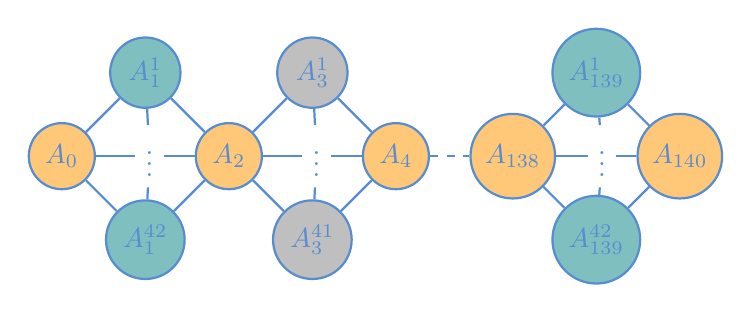
\begin{tikzpicture}[node distance={15mm}, thick, main/.style = {draw, circle}, cackithi] 
				\node[main, fill={rgb:orange,1;yellow,2;pink,5}] (1) {$A_0$}; 
				\node[main, fill= teal!50] (2) [above right of=1] {$A_1^1$}; 
				\node (3) [right = 5mm of 1] {$\vdots$};
				
				\node[main, fill= teal!50] (4) [below right of=1] {$A_1^{42}$}; 
				\node[main, fill={rgb:orange,1;yellow,2;pink,5}] (5) [below right of=2] {$A_2$}; 
				\node[main,fill=gray!50] (6) [above right of=5] {$A_3^1$}; 
				\node (7) [right = 5mm of 5] {$\vdots$};
				\node[main, fill=gray!50] (8) [below right of=5] {$A_3^{41}$}; 
				\draw (1) -- (2); 
				\draw (1) -- (3); 
				\draw (1) -- (4); 
				\draw (2) -- (3);
				\draw (3) -- (4);
				\draw (2) -- (5); 
				\draw (3) -- (5); 
				\draw (4) -- (5); 
				\draw (5) -- (6);
				\draw (5) -- (7);
				\draw (5) -- (8);   
				\draw (6) -- (7);
				\draw (7) -- (8);
				\node[main, fill={rgb:orange,1;yellow,2;pink,5}] (9) [below right of=6] {$A_4$};
				\draw (6) -- (9);
				\draw (7) -- (9); 
				\draw (8) -- (9);  
				\node[main, fill={rgb:orange,1;yellow,2;pink,5}] (10) [right = 5mm of 9] {$A_{138}$};
				\draw[dashed] (9) -- (10);  
				\node[main, fill= teal!50] (11) [above right of=10] {$A_{139}^1$}; 
				\node (12) [right = 4mm of 10] {$\vdots$}; 
				\node[main, fill= teal!50] (13) [below right of=10] {$A_{139}^{42}$}; 
				\draw (10) -- (11);
				\draw (10) -- (12);
				\draw (10) -- (13);
				\draw (11) -- (12);
				\draw (12) -- (13);
				\node[main, fill={rgb:orange,1;yellow,2;pink,5}] (14) [below right of=11] {$A_{140}$};
				\draw (11) -- (14);
				\draw (12) -- (14);
				\draw (13) -- (14);
			\end{tikzpicture}}
			\caption{\small\textit{\color{cackithi}Hình $1$. Hệ thống điểm quan sát với khoảng cách quan sát lớn nhất $140$. Mỗi điểm $A_i^{\bullet}$ thuộc tập $M_i$ có thể quan sát được tất cả điểm trong $M_{i-1}, M_{i+1}$ cũng như các điểm còn lại trong $M_i$.}}
			\vspace*{-10pt}
		\end{figure}
		\vskip 0.1cm		
		$\bullet$ Mỗi tập $M_{3k}$ và $M_{3k+2}$ với $k = 0, \ldots, 46$ chỉ chứa một điểm quan sát.
		\vskip 0.1cm
		$\bullet$ Mỗi tập $M_{1}$ và $M_{139}$ có $42$ điểm quan sát.
		\vskip 0.1cm
		$\bullet$ Mỗi tập $M_{3k+1}$ với $k = 1, \ldots, 45$ có $41$ điểm quan sát.
		\vskip 0.1cm
		Độc giả có thể kiểm tra rằng hệ thống này có $2023$ điểm quan sát và thỏa mãn điều kiện của bài toán. Ở đó, điểm quan sát duy nhất trong $M_{140}$ có khoảng cách quan sát $140$ tới điểm quan sát duy nhất trong $M_0$.
		\vskip 0.1cm
	\textbf{\color{cackithi}Câu $\pmb{3}$:} Cho tam giác $ABC$ với tâm đường tròn nội tiếp $I$. Gọi trung điểm của các cạnh $AC$ và $BC$ lần lượt là $M_b$ và $M_a$. Gọi giao điểm của đường thẳng $M_bI$ với đường thẳng $BC$ là $B'$ và giao điểm của đường thẳng $M_aI$ với đường thẳng $AC$ là $A'$. Biết rằng hai tam giác $ABC$ và $A'B'C$ có cùng diện tích. 
	\vskip 0.1cm
	Tìm giá trị có thể của góc $ACB$.\footnote{\color{cackithi}Trong số $09/2023$ chúng tôi đã sai sót khi yêu cầu tìm giá trị \textbf{\color{cackithi}lớn nhất} có thể của góc $ACB$. Thành thật xin lỗi các độc giả của Pi.}	
		\begin{figure}[H]
			\vspace*{-10pt}
			\centering
			\captionsetup{labelformat= empty, justification=centering}
			\resizebox{\columnwidth}{!}{\begin{tikzpicture}
				\tkzSetUpPoint[size=4,circle, fill= teal!50]
				\tkzDefPoints{0/0/A,6/0/B,0.8/4/C}
				
				\tkzDefTriangleCenter[centroid](A,B,C)
				\tkzGetPoint{G}
				\tkzDefSpcTriangle[medial](A,B,C){Ma,Mb,Mc}
				%\tkzLabelPoints(A,B,C)
				\tkzDefTriangleCenter[in](A,B,C)
				\tkzGetPoint{I}
				
				\tkzDefCircle[in](A,B,C) 
				\tkzGetPoints{I}{i}
				
				\tkzInterLL(Mb,I)(B,C)
				\tkzGetPoint{B1}
				\tkzInterLL(Ma,I)(A,C)
				\tkzGetPoint{A1}
				\tkzDrawSegments(A,B B,C C,A)
				\tkzDrawPoints(A1,B1)
				\tkzLabelPoint[above left](A1){$A'$}
				\tkzLabelPoint(B1){$B'$}
				\tkzDrawLines[dashed](B1,Mb A1,Ma)
				\tkzDrawSegments(B1,B A1,B1)
				\tkzDrawCircle(I,i)
				\tkzDrawPoints(I, Mb, Ma)
				
				\tkzDrawPoints(A,B,C)
				
				\tkzLabelPoint(I){$I$}
				
				\tkzLabelPoints[below left](A,Mb)
				\tkzLabelPoints[above right](B,Ma)
				\tkzLabelPoint[above](C){$C$}
			\end{tikzpicture}}
		\vspace*{-10pt}
		\end{figure}
		\textit{Lời giải.} Gọi độ dài các cạnh $AB$, $BC$ và $CA$ lần lượt là $c$, $a$, $b$. Đặt $\gamma \colon = \angle ACB$. Ta sẽ chứng minh rằng $\gamma = 60^{\circ}$.
		\vskip 0.1cm
		Thật vậy, từ $M_a$ vẽ đường thẳng song song với $AC$ và cắt $CI$ tại $P$. Vì $\angle CPM_a = \angle A'CI = \gamma/2$ nên tam giác $CM_aP$ cân tại $M_a$ và ta có $M_aP = M_aC = a/2 = M_aB$. Như vậy $P$ nằm trên đường tròn tâm $M_a$ bán kính $a/2$. Từ đó suy ra tam giác $BPC$ vuông tại $P$ và ta thu được 
		\begin{align*}
			CP = CB \cos (\gamma /2) = a \cos(\gamma/2).
		\end{align*}
		\begin{figure}[H]
			\vspace*{-5pt}
			\centering
			\resizebox{\columnwidth}{!}{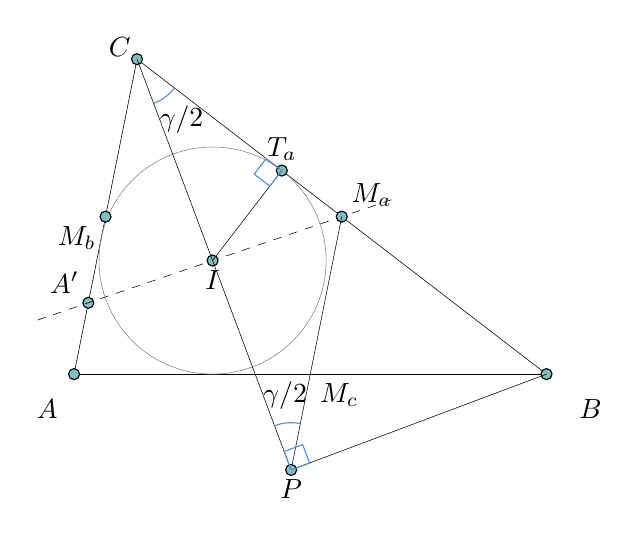
\begin{tikzpicture}[color= cackithi]
				\tkzSetUpPoint[size=4, fill= teal!50]
				
				\tkzDefPoints{0/0/A,6/0/B,0.8/4/C}
				
				\tkzDefTriangleCenter[centroid](A,B,C)
				\tkzGetPoint{G}
				\tkzDefSpcTriangle[medial](A,B,C){Ma,Mb,Mc}
				%\tkzLabelPoints(A,B,C)
				\tkzDefTriangleCenter[in](A,B,C)
				\tkzGetPoint{I}
				
				\tkzDefCircle[in](A,B,C) 
				\tkzGetPoints{I}{i}
				
				\tkzInterLL(Mb,I)(B,C)
				\tkzGetPoint{B1}
				\tkzInterLL(Ma,I)(A,C)
				\tkzGetPoint{A1}
				\tkzDrawSegments(A,B B,C C,A)
				\tkzDrawPoint(A1)
				\tkzLabelPoint[above left](A1){$A'$}
				\tkzDrawLine[dashed](A1,Ma)
				\tkzDrawCircle(I,i)
				\tkzDrawPoints(I, Mb, Ma)
				
				\tkzDrawPoints(A,B,C)
				
				\tkzLabelPoint(I){$I$}
				
				\tkzAutoLabelPoints[center = G](A,B,C)
				\tkzLabelPoint[below left](Mb){$M_b$}
				\tkzLabelPoint[above right](Ma){$M_a$}
				\tkzLabelPoint[below right](Mc){$M_c$}
				\tkzInterLL(C,I)(Ma,Mc)
				\tkzGetPoint{P}
				\tkzDrawSegments(C,P P,B Ma,P)
				\tkzDrawPoint(P)
				\tkzLabelPoint(P){$P$}
				\tkzDefPointBy[projection = onto C--B](I)
				\tkzGetPoint{Ta}
				\tkzDrawPoint(Ta)
				\tkzLabelPoint[above](Ta){$T_a$}
				\tkzDrawSegment(Ta,I)
				\tkzMarkRightAngles(C,Ta,I C,P,B)
				\tkzMarkAngle[size = 0.6, arc=l](P,C,B)
				\tkzLabelAngle[pos=0.95](P,C,B){$\gamma/2$}
				\tkzMarkAngle[size = 0.6, arc=l](Ma,P,C)
				\tkzLabelAngle[pos=0.95](Ma,P,C){$\gamma/2$}
			\end{tikzpicture}}
			\vspace*{-10pt}
		\end{figure}
		Gọi $T_a$ là điểm tiếp xúc của đường tròn nội tiếp tam giác $ABC$ với cạnh $BC$ thì $CT_a = (a+b-c)/2$. Do đó 
		\begin{align*}
			CI = \frac{CT_a}{\cos(\gamma/2)} = \frac{a+b-c}{2 \cos(\gamma/2)}
		\end{align*}
		và ta có
		\begin{align*}
		IP = CP - CI & =  a \cos(\gamma/2) - \frac{a+b-c}{2 \cos(\gamma/2)} \\
		& = \frac{2a \cos^2(\gamma/2) -a-b+c}{2 \cos(\gamma/2)} \\
		& = \frac{a[2\cos^2(\gamma /2)-1] - b +c}{2 \cos(\gamma/2)} \\
		& = \frac{a \cos (\gamma)-b+c}{2 \cos(\gamma/2)}.
		\end{align*}
		Vì $A'C \parallel M_aP$ nên theo định lý Thales 
		\begin{align*}
			\frac{CA'}{M_aP} = \frac{CI}{IP} & =  \frac{a+b-c}{a \cos(\gamma) - b +c} \\
			& = \frac{a+b-c}{a\frac{a^2 + b^2 -c^2}{2ab} -b +c} \\
			& = \frac{2b(a+b-c)}{a^2 + b^2 - c^2 - 2b^2 + 2bc} \\
			& = \frac{2b(a+b-c)}{a^2 - b^2 -c^2 + 2bc} \\
			& = \frac{2b(a+b-c)}{(a+c-b)(a+b-c)} \\
			& = \frac{2b}{a+c-b}
		\end{align*}
		và do đó
		\begin{align*} 
			\frac{CA'}{CB} = \frac{CA'}{2M_aP} = \frac{b}{a+c-b}. \tag{$3$}
		\end{align*}
		Hoán đổi vai trò của $A$ với $B$ (do đó $M_a$ với $M_b$, $a$ với $b$, $A'$ với $B'$) ta thu được
		\begin{align*} 
			\frac{CB'}{CA} = \frac{a}{b+c-a}. \tag{$4$}
		\end{align*}
		Từ giả thiết hai tam giác $ABC$ và $A'B'C$ có cùng diện tích ta có
		\begin{align*}
			\frac{CA'}{CB} = \frac{CA}{CB'}.
		\end{align*}
		Kết hợp với ($3$) và ($4$) ta nhận được
		\begin{align*}
			&\frac{b}{a+c-b}  = \frac{b+c-a}{a} \\
			\Leftrightarrow \,&ab  = (a+c-b)(b+c-a) \\
			\Leftrightarrow \,&ab  = c^2 - (a-b)^2 \\
			\Leftrightarrow \,&c^2 = a^2 + b^2 - ab.
		\end{align*}
		Từ hệ thức $c^2 = a^2 + b^2 - 2 ab \cos(\gamma)$ suy ra $\cos(\gamma) = \frac{1}{2}$. Do đó $\gamma = 60^{\circ}$.
	\vskip 0.1cm
	\textbf{\color{cackithi}Câu $\pmb{4}$}: Cho một đa giác đều $2n$ cạnh. Trong các đoạn thẳng nối các đỉnh của đa giác (cạnh biên hoặc đường chéo) ta tô $n$ đoạn màu đỏ sao cho:
	\vskip 0.1cm
	$1.$ Các điểm cuối của các đoạn màu đỏ chính là $2n$ đỉnh của đa giác.
	\vskip 0.1cm
	$2.$ Không có $2$ đoạn màu đỏ nào có độ dài bằng nhau.
	\vskip 0.1cm
	Tìm tất cả các số tự nhiên $n \ge 2$ sao cho tồn tại một phép tô màu thỏa mãn yêu cầu bên trên.
	\vskip 0.1cm	
	\textit{Lời giải.}
	Ta sẽ chứng minh rằng một cách tô màu như vậy tồn tại khi và chỉ khi $n \equiv 0 \mod 4$ hoặc $n \equiv 1 \mod 4$.
	\vskip 0.1cm
	$``\Rightarrow":$ Giả sử tồn tại cách tô màu như vậy. Gọi $2n$ đỉnh của đa giác là $A_1, A_2, \ldots, A_{2n}$, được sắp xếp theo chiều kim đồng hồ. Ta định nghĩa \textit{khoảng cách $d(i,j)$ giữa hai đỉnh $A_i, A_j$} là số cạnh nằm trên đường đi ngắn nhất dọc theo các cạnh biên của đa giác nối hai đỉnh này. Khoảng cách này sẽ lấy một trong các giá trị trong tập $\{1,2\ldots,n\}$. Chẳng hạn, với $n=4$ như trong Hình $2$ thì $d(1,4) = 3$ và $d(1,7) = 2$. 
	\vskip 0.1cm
	Dễ thấy
	\begin{align*}
		A_iA_j = 2r \sin\frac{d(i,j)\pi}{2n}
	\end{align*}
	với $r$ là khoảng cách từ đỉnh đến tâm của đa giác. Do đó, $A_iA_j > A_rA_s \iff d(i,j) > d(r,s)$. Bởi vậy ta có thể thay yêu cầu rằng không có hai đoạn màu đỏ nào có cùng độ dài bằng yêu cầu không có hai cặp đỉnh nào có cùng khoảng cách.
	\vskip 0.1cm	
	Biểu diễn mỗi cặp đỉnh $(A_i, A_j)$ bởi cặp chỉ số $(i,j)$. Ta có thể giả sử $i <j$. Bài toán đã cho tương đương với việc phân hoạch tập $2n$ số tự nhiên $\{1,2,\ldots, 2n\}$ thành $n$ cặp $\{(i_k,j_k)\}_{k = 1}^n$ với $i_k<j_k$ sao cho tập các khoảng cách $\{d(i_k,j_k)\}_{k=1}^n$ là $\{1, \ldots, n\}$. Ta có
	\begin{align*}
		\hspace*{-10pt}d(i_k,j_k) \!\!=\!\! 
		\begin{cases}
			\!\!j_k\!-\!i_k, \text{ nếu } j_k\!-\!i_k \!\le\! n \\
			\!\!2n\!-\! j_k \!+\! i_k, \text{ nếu } j_k\!-\!i_k \!>\! n.
		\end{cases}\hspace*{-10pt} \tag{$5$}
	\end{align*}
	Bằng cách hoán đổi $i_k$ với $j_k$ trong trường hợp $j_k-i_k > n$ ta có 
	\begin{align*} 
			\sum_{k=1}^{n}j_k - \sum_{k=1}^n i_k = &\sum_{k=1}^nd(i_k,j_k) + 2ns\\
			 = &\sum_{k=1}^ni + 2ns \\
			 = &n(n+1)/2 + 2ns.\tag{$6$}
		\end{align*}
		với $s$ là số trường hợp $j_k-i_k > n$. Mặt khác,
		\begin{align*}
			\sum_{k=1}^nj_k + \sum_{k=1}^ni_k &= \sum_{k=1}^{2n}i \\
			&= 2n(2n+1)/2. \tag{$7$}
		\end{align*}
		Từ các phương trình ($6$) và ($7$) ta thu được 
		\begin{align*}
			\sum_{k=1}^{n}j_k = \frac{n(5n+3)}{4} + ns.
		\end{align*}
		Vì $\sum_{k=1}^{n}j_k \in \mathbb{N}$ nên $\frac{n(5n+3)}{4} \in \mathbb{Z}$. Từ đó suy ra $n \equiv 0 \mod 4$ hoặc $n \equiv 1 \mod 4$.
		\vskip 0.1cm
		$``\Leftarrow":$
		\vskip 0.1cm
		\underline{\textit{Trường hợp $n \equiv 0 \mod 4$.}} Đặt $n = 4k$.
		\vskip 0.1cm
		$\bullet$ Với $k=1$ ta có thể tô màu như Hình $2$.
			\begin{figure}[H]
%				\vspace*{-10pt}
				\centering
				\captionsetup{labelformat= empty, justification=centering}
				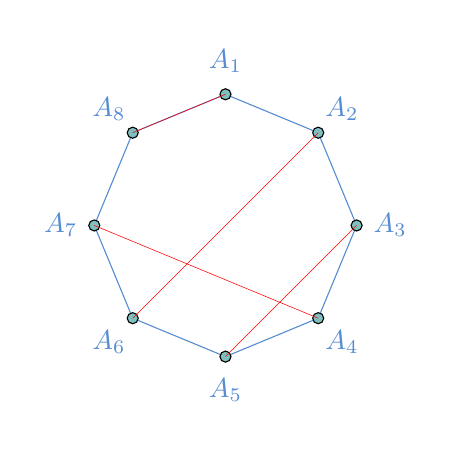
\begin{tikzpicture}[cackithi,scale = 0.75]
					\tkzSetUpPoint[size=4, fill= teal!50]
					\def\laenge{1.7}
					\def\n{8}
					\pgfmathtruncatemacro\w{360/\n}
					\draw
					(0:0) coordinate (A1)
					foreach \i in {2,...,\n}
					{--++(360+\w/2-\i*\w +\w:\laenge) coordinate (A\i)}
					--cycle;
					\tkzDrawPoints(A1,A...,A8)
					\foreach \i in {1,...,\n}\node[anchor={270-\i*\w +\w}, circle] at (A\i){$A_{\i}$};
					\tkzDrawSegment[red](A1,A8)
					\tkzDrawSegment[red](A2,A6)
					\tkzDrawSegment[red](A3,A5)
					\tkzDrawSegment[red](A4,A7)
				\end{tikzpicture}
				\caption{\small\textit{\color{cackithi}Hình $2$. Đa giác đều $8$ cạnh.}}
				\vspace*{-10pt}
			\end{figure}
			$\bullet$ Với $k \ge 2$ thì danh sách các đoạn màu đỏ cùng với khoảng cách giữa các đỉnh (phương trình ($5$) với $2n = 8k$) được cho trong bảng dưới đây:
		\begin{center}
			\resizebox{\linewidth}{!}{%
				\begin{tabular}{ |c|c|c| } 
					\hline
					Chỉ số & Cạnh & Khoảng cách \\ 
					\hline
					$1 \le i \le k$ & $(i, 8k+1-i)$ & $1,3, \ldots, 2k-1$ \\ 
					\hline
					$i = k+1$ & $(k+1, 5k+1)$ & $4k$ \\
					\hline
					$k+2 \le i \le 2k$ & $(i, 8k+2-i)$ & $2k+2, 2k+4, \ldots, 4k-2$ \\ 
					\hline
					$i = 2k+1$ & $(2k+1,4k+1)$ & $2k$ \\
					\hline
					$2k+2 \le i \le 3k+1$ & $(i, 8k+3-i)$ & $4k-1, 4k-3,\ldots, 2k+1$ \\
					\hline
					$3k+2 \le i \le 4k$ & $(i, 8k+2-i)$ & $2k-2, \ldots, 2$ \\
					\hline
			\end{tabular}}
		\end{center}
		\begin{figure}[H]
%			\vspace*{-5pt}
			\centering
			\captionsetup{labelformat= empty, justification=centering}
			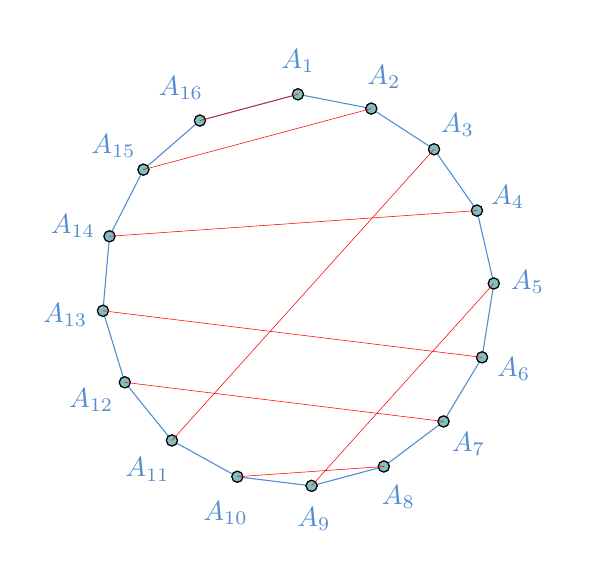
\begin{tikzpicture}[cackithi,scale = 0.95]
				\tkzSetUpPoint[size=4, fill= teal!50]
				\def\laenge{1}
				\def\n{16}
				\pgfmathtruncatemacro\w{360/\n}
				\draw
				(0:0) coordinate (A1)
				foreach \i in {2,...,\n}
				{--++(360+\w/2-\i*\w +\w:\laenge) coordinate (A\i)}
				--cycle;
				\tkzDrawPoints(A1,A...,A16)
				\foreach \i in {1,...,\n}\node[anchor={270-\i*\w +\w}, circle] at (A\i){$A_{\i}$};
				\tkzDrawPoints(A1,A...,A16)
				\tkzDrawSegment[red](A1,A16)
				\tkzDrawSegment[red](A2,A15)
				\tkzDrawSegment[red](A3,A11)
				\tkzDrawSegment[red](A4,A14)
				\tkzDrawSegment[red](A5,A9)
				\tkzDrawSegment[red](A6,A13)
				\tkzDrawSegment[red](A7,A12)
				\tkzDrawSegment[red](A8,A10)
			\end{tikzpicture}
			\caption{\small\textit{\color{cackithi}Hình $3$. Đa giác đều $16$ cạnh.}}
			\vspace*{-15pt}
		\end{figure}
		\underline{\textit{Trường hợp $n \equiv 1 \mod 4$.}} Đặt $n = 4k+1$. 
		\vskip 0.1cm
		$\bullet$ Với $k=1$ ta có thể tô màu như Hình $4$.
		\begin{figure}[H]
			\vspace*{-10pt}
			\centering
			\captionsetup{labelformat= empty, justification=centering}
			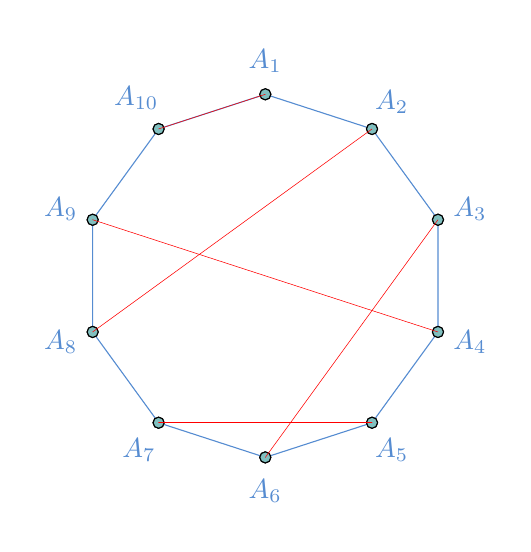
\begin{tikzpicture}[cackithi,scale = 0.95]
				\tkzSetUpPoint[size=4, fill= teal!50]
				\def\laenge{1.5}
				\def\n{10}
				\pgfmathtruncatemacro\w{360/\n}
				\draw
				(0:0) coordinate (A1)
				foreach \i in {2,...,\n}
				{--++(360+\w/2-\i*\w +\w:\laenge) coordinate (A\i)}
				--cycle;
				\tkzDrawPoints(A1,A...,A10)
				\foreach \i in {1,...,\n}\node[anchor={270-\i*\w +\w}, circle] at (A\i){$A_{\i}$};
				\tkzDrawPoints(A1,A...,A10)
				\tkzDrawSegment[red](A1,A10)
				\tkzDrawSegment[red](A2,A8)
				\tkzDrawSegment[red](A3,A6)
				\tkzDrawSegment[red](A4,A9)
				\tkzDrawSegment[red](A5,A7)
			\end{tikzpicture}
			\caption{\small\textit{\color{cackithi}Hình $4$. Đa giác đều $10$ cạnh.}}
			\vspace*{-15pt}
		\end{figure}
		$\bullet$  Với $k \ge 2$ thì danh sách các đoạn màu đỏ cùng với khoảng cách giữa các đỉnh (phương trình ($5$) với $2n = 8k+2$) được cho trong bảng dưới đây:
		\begin{center}
			\resizebox{\linewidth}{!}{%
				\begin{tabular}{ |c|c|c| } 
					\hline
					Chỉ số & Cạnh & Khoảng cách \\ 
					\hline
					$1 \le i \le k$ & $(i, 8k+3-i)$ & $1,3, \ldots, 2k-1$ \\ 
					\hline
					$i = k+1$ & $(k+1, 5k+3)$ & $4k$ \\
					\hline
					$k+2 \le i \le 2k$ & $(i, 8k+4-i)$ & $2k+2, 2k+4, \ldots, 4k-2$ \\ 
					\hline
					$i = 2k+1$ & $(2k+1, 4k+2)$ & $2k+1$ \\
					\hline
					$2k+2 \le i \le 3k+1$ & $(i, 8k+5-i)$ & $4k+1, 4k-1,\ldots, 2k+3$ \\
					\hline
					$3k+2 \le i \le 4k+1$ & $(i,8k+4-i)$ & $2k, \ldots, 2$ \\
					\hline
			\end{tabular}}
		\end{center}
\end{multicols}
\newpage
\begingroup
\AddToShipoutPicture*{\put(150,700){\includegraphics[scale=1]{../tieude1.pdf}}}
\centering
\endgroup
\vspace*{3pt}

\begin{multicols}{2}
	Trong phần đầu chuyên mục, chúng tôi sẽ trình bày với các bạn lời giải các bài toán trong kỳ thi Olympic toán Tuymaada năm $2022$ của nước cộng hòa Sakha (Yakutia), thuộc Liên bang Nga đăng trong số tháng $5/2023$. 
	\begin{figure}[H]
		\vspace*{-5pt}
		\centering
		\captionsetup{labelformat= empty, justification=centering}
		\includegraphics[width= 1\linewidth]{gocolympic}
%		\caption{\small\textit{\color{}.}}
		\vspace*{-15pt}
	\end{figure}
	{\bf\color{cackithi} OC$\pmb{46.}$} Arnim và Brentano có một chiếc bình nhỏ đựng $1500$ viên kẹo trên bàn và một túi lớn đựng kẹo dự phòng dưới gầm bàn. Họ thay phiên nhau chơi một trò chơi với Arnim bắt đầu trước. Ở mỗi lượt đi, người chơi có thể ăn $7$ viên kẹo trong bình hoặc lấy 6 viên kẹo từ túi bên dưới và thêm chúng vào bình. Người chơi không được lấy kẹo trong túi dưới gầm bàn hai lần liên tiếp. Người chơi được tuyên bố là người chiến thắng nếu làm cho chiếc bình rỗng sau lượt chơi của mình. Trong mọi trường hợp khác, nếu
	một người chơi không thể thực hiện được nước đi trong lượt của mình, trò chơi được tuyên bố là hòa. Liệu người nào có chiến lược để luôn chiến thắng?
	\vskip 0.1cm
	\textit{Lời giải.} Ban đầu trong bình có $1500$ viên kẹo. Brentano có chiến lược để luôn thắng bằng cánh đảm bảo rằng nếu trước lượt đi của Arnim trong bình có $15k$ viên kẹo, thì sau khi mỗi người đi $2$ lượt, trong bình sẽ còn lại $15(k-1)$ viên kẹo. 
	\vskip 0.1cm
	Cụ thể là nếu trong lượt đi thứ nhất của mình Arnim thêm $6$ viên kẹo vào bình thì ở lượt đi sau anh ta phải ăn $7$ viên. Do đó Brentano sẽ ăn $7$ viên kẹo trong cả $2$ lượt đi của mình và số kẹo trong bình sau đó là $15k+6-7-7-7=15(k-1).$ Nếu trong lượt đi thứ nhất của mình Arnim  ăn $7$ viên thì Brentano cũng ăn $7$ viên trong lượt thứ nhất. 
	Đến lượt đi thứ $2$ nếu Arnim ăn $7$ viên thì sau đó Brentano thêm vào $6$ viên và số kẹo trong bình còn lại là $15k-7-7-7+6=15(k-1).$    Còn nếu đến lượt thứ $2$ Arnim thêm vào 6 viên thì sau đó Brentano sẽ ăn $7$ viên và số kẹo trong bình còn lại là $15k-7-7+6-7=15(k-1).$ Như vậy sau khi mỗi người đi $200$ lượt thì Brentano là người chiến thắng.
	\vskip 0.1cm
	{\bf\color{cackithi}OC$\pmb{47.}$}  Cho $M$ là trung điểm của cạnh $A$B trong tam giác đều $ABC.$ Điểm $D$ thuộc cạnh $BC$ sao cho $BD : DC = 3 : 1.$ Giả sử $T$ là điểm trên đường thẳng đi qua $C$ và song song với $MD$ sao cho $\angle CTA = 150^\circ.$ Tìm số đo $\angle MTD.$
	\begin{figure}[H]
		\vspace*{-5pt}
		\centering
		\captionsetup{labelformat= empty, justification=centering}
		\definecolor{qqwuqq}{rgb}{0.,0.39215686274509803,0.}
		\definecolor{uuuuuu}{rgb}{0.26666666666666666,0.26666666666666666,0.26666666666666666}
		\definecolor{ududff}{rgb}{0.30196078431372547,0.30196078431372547,1.}
		\begin{tikzpicture}[cackithi,scale=1.2,node font=\small]
			\draw[color=uuuuuu] (1.8771681255350392,1.9481399025612232) -- (1.90851486019539,2.1110223138105475) -- (1.7456324489460657,2.1423690484708984) -- (1.7142857142857149,1.979486637221574) -- cycle; 
			\draw [shift={(1.7142857142857149,1.979486637221574)},color=qqwuqq,fill=qqwuqq,fill opacity=0.10000000149011612] (0,0) -- (-130.8933946491309:0.23457748258628952) arc (-130.8933946491309:-10.893394649130876:0.23457748258628952) -- cycle;
			\draw  (2.,0.) circle (2.cm);
			\draw  (2.,3.4641016151377553)-- (2.5,2.5980762113533165);
			\draw  (2.3109450177226596,3.0662755356334794) -- (2.1890549822773426,2.9959022908575927);
			\draw  (3.,1.7320508075688776)-- (2.5,2.5980762113533165);
			\draw  (2.689054982277343,2.129876887073154) -- (2.8109450177226605,2.2002501318490406);
			\draw  (3.,1.7320508075688776)-- (3.5,0.8660254037844388);
			\draw  (3.3109450177226583,1.3342247280646016) -- (3.1890549822773413,1.263851483288715);
			\draw  (3.5,0.8660254037844388)-- (4.,0.);
			\draw  (3.8109450177226587,0.4681993242801627) -- (3.6890549822773417,0.3978260795042762);
			\draw  (0.,0.)-- (2.,0.);
			\draw  (0.9706778146767137,0.07037324477588658) -- (0.9706778146767137,-0.07037324477588658);
			\draw  (1.029322185323286,0.07037324477588658) -- (1.029322185323286,-0.07037324477588658);
			\draw  (2.,0.)-- (4.,0.);
			\draw  (2.9706778146767134,0.07037324477588658) -- (2.9706778146767134,-0.07037324477588658);
			\draw  (3.0293221853232857,0.07037324477588658) -- (3.0293221853232857,-0.07037324477588658);
			\draw  (2.5,2.5980762113533165)-- (2.,0.);
			\draw  (3.,1.7320508075688776)-- (2.,0.);
			\draw  (2.5756061103843018,0.8562325387809366) -- (2.453716074938985,0.9266057835568232);
			\draw  (2.5462839250610156,0.8054450240120545) -- (2.4243938896156987,0.8758182687879411);
			\draw  (1.7142857142857149,1.979486637221574)-- (3.,1.7320508075688776);
			\draw  (2.,3.4641016151377553)-- (1.7142857142857149,1.979486637221574);
			\draw  (1.7142857142857149,1.979486637221574)-- (0.,0.);
			\draw  (2.,0.)-- (1.7142857142857149,1.979486637221574);
			\draw  (1.7916802919345747,0.9506685609177279) -- (1.9309831895863658,0.9707752022822663);
			\draw  (1.7833025246993495,1.0087114349393076) -- (1.9226054223511404,1.0288180763038461);
			\draw  (1.7142857142857149,1.979486637221574)-- (2.5,2.5980762113533165);
			\draw  (2.0636107016266734,2.3440746880399277) -- (2.1506750126590424,2.233488160534963);
%			\begin{scriptsize}
				\draw [fill=white] (0.,0.) circle (1.5pt);
				\draw[color=ududff] (-0.17754689709133267,-0.15347137061022087) node {$A$};
				\draw [fill=white] (4.,0.) circle (1.5pt);
				\draw[color=ududff] (4.23250977553091,-0.16520024473953532) node {$B$};
				\draw [fill=white] (2.,3.4641016151377553) circle (1.5pt);
				\draw[color=uuuuuu] (2.086125809866361,3.6818704696755975) node {$C$};
				\draw [fill=white] (2.,0.) circle (1.5pt);
				\draw[color=uuuuuu] (2.0157525650904744,-0.21211574125679306) node {$M$};
				\draw [fill=white] (3.,1.7320508075688776) circle (1.5pt);
				\draw[color=uuuuuu] (3.1769111038926074,1.922539350278433) node {$R$};
				\draw [fill=white] (2.5,2.5980762113533165) circle (1.5pt);
				\draw[color=uuuuuu] (2.649111768073456,2.8022049099770157) node {$D$};
				\draw [fill=white] (3.5,0.8660254037844388) circle (1.5pt);
				\draw[color=uuuuuu] (3.3763019640909535,0.6558209443124747) node {$F$};
				\draw [fill=white] (1.7142857142857149,1.979486637221574) circle (1.5pt);
				\draw[color=uuuuuu] (1.5935130964351534,2.1688457069940363) node {$R'$};
				\draw (2.2386011735474494,1.7700639865973455) node[below] {$120^{\circ}$};
%			\end{small}
		\end{tikzpicture}
		\vspace*{-5pt}
	\end{figure}
	\textit{Lời giải.} Gọi $\ell$ là đường thẳng đi qua $C$ song song với $MD.$ Giả sử đường tròn đường kính $AB$ cắt $BC$ tại $R$ và cắt $\ell$ tại $R'.$  Ta sẽ chứng minh  $R'$ trùng với  $T.$ 
	\vskip 0.1cm
	Dễ thấy tam giác cân $MBR$ có góc $\angle MBR=60^\circ$ nên nó là tam giác đều. Do đó $R$ là trung điểm $BC$ và $D$ là trung điểm $RC.$ Trong tam giác $CRR',$ $MD$ đi qua trung điểm của $CR$ và song song $CR'$ nên nó phải đi qua trung điểm của $RR'.$ Do $MD$ là đường kính, ta suy ra $MD\perp RR'.$ Do $CR'$ song song với $MD,$ ta suy ra $\angle CR'R=90^\circ.$ 
	\vskip 0.1cm
	Mặt khác, do $\angle AR'R=180^\circ - \angle ABR= 180^\circ-60^\circ=120^\circ,$ ta có 
	\begin{align*}
		\angle AR'C&=360^\circ-\angle AR'R - \angle CR'R \\
		&= 360^\circ -120^\circ - 90^\circ=150^\circ.
	\end{align*}
	Như vậy $R'$ trùng với $T.$ Do $R$ và $R'$ đối xứng nhau qua $MD$ ta có $\angle MR'D=\angle MRD= 120^\circ.$  Như vậy $\angle MTD=120^\circ.$  
	\vskip 0.1cm
	{\bf\color{cackithi} OC$\pmb{48.}$} Cho các số nguyên $a, b, c$ và số nguyên tố lẻ $p.$ Chứng minh rằng tồn tại các số nguyên $x$ và $y$ sao cho $p$ là ước của $x^2 + y^2 + ax + by + c.$      
	\vskip 0.1cm
	\textit{Lời giải.}
	Khi tính giá trị  $f(x)=x^2+ax+c$ modulo $p,$ với $x \in \{0, 1, \cdots, p - 1\}$ ta được ít nhất $\frac{p+1}{2}$  số phân biệt. Thật vậy, nếu $x_1$ và $x_2$ là hai số nguyên phân biệt nằm giữa $0$ và $p-1$, và $p$ là ước của  $f(x_1)-f(x_2) = x_1^2 +ax_1+c-(x_2^2 +ax_2+c) = (x_1-x_2)(x_1+x_2+a)$,
	thì $p$ cũng là ước của $x_1 + x_2 + a$, nghĩa là với mỗi $x_1\in \{0, 1, \cdots, p - 1\}$ có nhiều nhất
	một $x_2\in \{0, 1, \cdots, p - 1\}$  sao cho $f(x_2)\equiv f(x_1) \mod p.$ 
	\vskip 0.1cm
	Lập luận tương tự cho thấy các giá trị của đa thức $g(y) = -y^2 - by$ với  $y \in \{0, 1, \cdots, p - 1\}$ ta cũng nhận được ít nhất $\frac{p+1}{2}$ số phân biệt modulo $p.$ Như vậy, ta có hai tập các số dư modulo $p,$  mỗi tập có nhiều hơn $\frac{p}{2}$ số dư, do đó hai tập này phải có ít nhất một phần tử chung. Ta suy ra $p$ là ước của $f(x) - g(y)$ với các số nguyên $x$ và $y$ nào đó. Ta được điều cần chứng minh.  
	\vskip 0.1cm
	Trong phần cuối của chuyên mục kỳ này, chúng tôi sẽ giới thiệu với bạn đọc ba bài toán chọn lọc trong kỳ thi Olympic toán vùng Trung Mỹ và Caribê năm $2023$. Các bài toán này phù hợp với trình độ học sinh lớp $8-10$.
	\vskip 0.1cm
	{\bf\color{cackithi} OC$\pmb{55.}$} Tìm tất cả các cách tô màu các số nguyên dương sao cho điều kiện sau thỏa mãn:  
	\vskip 0.1cm
	$\bullet$ Mỗi số có màu xanh hoặc đỏ;
	\vskip 0.1cm
	$\bullet$ Tổng của hai số (không nhất thiết phân biệt) cùng màu bất kỳ  có màu xanh.
	\vskip 0.1cm
	{\bf\color{cackithi} OC$\pmb{56.}$} Octavio viết một số nguyên dương $n$ lên bảng  và sau đó anh bắt đầu một quá trình trong đó, ở mỗi bước, anh xóa số nguyên $k$ được viết trên bảng  và thay thế nó bằng một trong các số sau:
	\begin{align*}
		3k-1, \quad 2k+1, \quad \frac{k}{2},
	\end{align*}
	với điều kiện số mới viết là số nguyên.
	\vskip 0.1cm
	Chứng minh rằng với mọi số nguyên dương $n$, Octavio có thể viết lên bảng  số $3^{2023}$ sau hữu hạn bước.
	\vskip 0.1cm
	{\bf\color{cackithi} OC$\pmb{57.}$} Trong một cái ao có $n (n \geq 3)$  hòn đá  xếp thành vòng tròn. Một công chúa muốn đánh số những hòn đá với các số $1, 2, \dots, n$ theo thứ tự nào đó rồi đặt một số con cóc lên những hòn đá. Sau khi đặt tất cả các con cóc vào vị trí, chúng bắt đầu nhảy theo quy tắc sau: khi một con cóc đến hòn đá có đánh số $k$, nó đợi $k$ phút rồi nhảy sang hòn đá liền kề theo chiều kim đồng hồ.
	\vskip 0.1cm
	Hỏi số lượng cóc nhiều nhất là bao nhiêu để công chúa có thể đánh số các hòn đá và đặt các con cóc sao cho không bao giờ có hai con cóc ở trên cùng một hòn đá trong thời gian từ một phút trở lên?
\end{multicols}
%	\newpage
%
	\setcounter{figure}{0}
	\thispagestyle{lichsutoanhocnone}
\pagestyle{lichsutoanhoc}
\graphicspath{{../lichsutoanhoc/pic2/}}
\everymath{\color{lichsutoanhoc}}
\blfootnote{$^1$\color{lichsutoanhoc}THPT chuyên Hà Nội -- Amsterdam.}
\begingroup
\AddToShipoutPicture*{\put(0,616){\includegraphics[width=19.3cm]{../bannerlichsu}}}
\AddToShipoutPicture*{\put(88,550){\includegraphics[scale=1]{../tieude2.pdf}}}
\centering
\endgroup

\vspace*{155pt}

\begin{multicols}{2}		
	Một ý tưởng tưởng chừng như mâu thuẫn với những cảm quan thường thức, thế nhưng lại trở thành một vũ trụ hình học mới lạ và chặt chẽ, và có thể nắm giữ bản chất của không gian chúng ta đang sống. Thế nhưng quá trình khám phá và phát triển ý tưởng ấy phải trải qua hàng thập kỷ với nhiều trắc trở và gian nan.
	\vskip 0.1cm
	\textbf{\color{lichsutoanhoc}Hy Lạp và Saccheri}
	\vskip 0.1cm
	Một trong những thứ mà người Hy Lạp cổ đại có thể tự hào với toàn thế giới chắc chắn là Toán học của họ, đặc biệt là Hình học phát triển bậc nhất nhân loại đương thời. Không chỉ những tính toán và đo đạc của họ có độ chính xác cao, hệ thống lý thuyết Hình học của họ cũng được thiết lập hết sức chặt chẽ, một điều hiếm thấy ở các nền văn minh đương thời. Minh chứng rõ ràng nhất chính là bộ ``Elements of Geometry" hay ``Elements" (Cơ sở) của Euclid thành Alexandria. Tác phẩm là một bản tổng hợp các kiến thức tự cổ chí kim của nền Hình học Hy Lạp đồ sộ, được sắp xếp theo trình tự khoa học, và quan trọng nhất: có sự xuất hiện của tiên đề, một số ít các mệnh đề được thừa nhận, để các kết quả sau đó được phát triển chỉ dựa trên những tiên đề ấy. Dù lý luận chưa kín kẽ hoàn toàn, một số chứng minh vẫn còn những điều được ngầm thừa nhận và một số vẫn phụ thuộc vào hình vẽ, và các tiên đề vẫn chưa đầy đủ (về sau ta sẽ chỉ ra những lỗi này) ``Elements" vẫn là một tác phẩm để đời của nhà sư phạm lỗi lạc. 
	\begin{figure}[H]
		\vspace*{-5pt}
		\centering
		\captionsetup{labelformat= empty, justification=centering}
		\includegraphics[width= 1\linewidth]{Sir_Henry_Billingsley's_first_English_version_of_Euclid's_Elements,_1570.png}
		%		\caption{\small\textit{\color{}}}
		\vspace*{-15pt}
	\end{figure}
	Ngoài việc Hình học được đặt trên nền móng logic như trên, đã có hẳn một phái nghiên cứu những ý nghĩa huyền bí của nó, đứng đầu bởi không ai khác ngoài Pythagoras xứ Samos. Trong số những giáo lý của triết gia bí ẩn này tới các môn đồ, Toán học giữ một vai trò cực kỳ quan trọng trong mục đích hàng đầu của họ -- hiểu thêm về thực tại và triết lý. Những con số (với phái này ``số" là các số nguyên dương khác $1$) được cho là ẩn chứa những lời giải thích về bản chất của vũ trụ, từ đó dẫn đến cách mô tả đậm chất Thần số học của họ. Hình học Euclid lại được coi là mô tả chính xác cho không gian thực. Quan điểm này sẽ trở thành niềm tin chủ đạo của giới học thuật châu Âu, do sự tiếp thu tri thức từ Hy Lạp cổ đại.
	\vskip 0.1cm
	Quay lại với Euclid, các tiên đề ông đưa ra sẽ là trọng tâm của chúng ta trong phần tới, đặc biệt là tiên đề cuối. Chúng lần lượt là:
	\vskip 0.1cm
	$1.$ Qua hai điểm bất kì, luôn luôn vẽ được một đường thẳng.
	\vskip 0.1cm
	$2.$ Có thể kéo dài một đoạn thẳng một đoạn dài hữu hạn theo hai hướng.
	\vskip 0.1cm
	$3.$ Với một điểm và một đoạn bất kỳ, luôn luôn vẽ được một đường tròn có tâm và bán kính lần lượt là điểm và có độ dài bằng đoạn đã nêu. 
	\vskip 0.1cm
	$4.$ Mọi góc vuông đều bằng nhau. Góc vuông được định nghĩa là góc bằng với góc bù của nó.
	\vskip 0.1cm
	$5.$ Nếu $2$ đường thẳng tạo với $1$ đường thẳng thứ $3$ hai góc trong cùng phía mà có tổng nhỏ hơn hai góc vuông thì chúng sẽ cắt nhau về phía đó, khi cả hai được kéo dài vô hạn.
	\vskip 0.1cm
	và $5$ định đề (common notion):
	\vskip 0.1cm
	$1.$ Hai cái cùng bằng cái thứ ba thì bằng nhau. 
	\vskip 0.1cm
	$2.$ Thêm những cái bằng nhau vào những cái bằng nhau thì được những cái bằng nhau.
	\vskip 0.1cm
	$3.$ Bớt đi những cái bằng nhau từ những cái bằng nhau thì được những cái bằng nhau.
	\vskip 0.1cm
	$4.$ Trùng nhau thì bằng nhau.
	\vskip 0.1cm
	$5.$ Toàn thể lớn hơn một phần.
	\vskip 0.1cm
	Trước khi đi tiếp, chúng ta cần hai kết quả đáng lưu tâm trong Elements ở đây:
	\vskip 0.1cm
	Định lý $16$ của ``Elements" Quyển I, tên khác là định lý góc ngoài, một dạng yếu hơn của định lý góc ngoài ta quen biết nhưng không cần tới tiên đề song song, khẳng định: 
	\vskip 0.1cm
	Trong một tam giác bất kỳ, góc ngoài của một đỉnh nào đó thì lớn hơn hai góc ở hai đỉnh còn lại.
	\vskip 0.1cm
	Khi thừa nhận thêm tiên đề $5$ thì góc ngoài sẽ bằng tổng hai góc ở hai đỉnh ấy luôn.
	\vskip 0.1cm
	Định lý $27$, định lý về góc so le trong: 
	\vskip 0.1cm
	Hai đường thẳng có một đường thứ ba cắt qua mà tạo với đường thứ ba hai góc so le trong bằng nhau thì là hai đường song song.
	\vskip 0.1cm
	Hai định lý này (cùng một số mệnh đề ngầm được thừa nhận) đã chỉ ra sự tồn tại của hai đường thẳng song song, và có thể được chứng minh mà không sử dụng tiên đề số $5$. Ba định đề đầu tiên còn đúng cả trong số học, trong khi định đề thứ $5$ có một câu chuyện riêng, ta để dành lúc khác. Nên nhớ rằng, theo cách hiểu được duy trì trong thời gian dài, một tiên đề là một sự thật tự nó hiển nhiên. 
	\vskip 0.1cm
	Không khó để thấy tiên đề cuối cùng trông phức tạp hơn nhiều so với những tiên đề còn lại. Nó được trình bày dưới dạng giả thiết -- kết luận, rồi còn chứa trong đó một giả sử hơi khó hình dung -- hai đường được kéo dài vô hạn, dù hành động này trên thực tế là không thể kiểm chứng. Vì thế không ít người đã nghi ngờ rằng đây thực chất là một định lý, và không ít trong số họ đã đổ thời gian và tâm sức vào nhằm đưa ra một chứng minh thỏa đáng. Hẳn rồi, nếu một trong các nỗ lực đó chính xác thì đã chẳng có bài viết này, tất cả đều không tránh được lỗi ngầm thừa nhận một khẳng định nào đó hóa ra lại tương đương với tiên đề $5$. Vậy là, kể từ khi thời Euclid, cho đến giai đoạn thất thoát sách vở Hy Lạp cổ đại, để rồi được những người Ả Rập tìm thấy và dựa vào đó đến phát triển, tới khi những lái buôn nơi đây đem Toán của mình tới châu Âu trong những cuộc giao thương, góp phần đánh thức nền Toán học chìm trong đêm dài Trung Cổ, cho tới mấy trăm năm ``Elements" làm cuốn sách hình học mẫu mực trên lục địa, sau bao nhiêu thế hệ trí thức chung tay giải quyết, thứ hậu thế thu được từ các chứng minh sai lầm hầu như chỉ là các phát biểu lại của tiên đề cuối cùng. 
	\vskip 0.1cm
	Điều này không có nghĩa là công sức của họ là vô ích hoàn toàn, ngược lại, đây là một sự chuẩn bị cần thiết cho những diễn biến tới. Hãy cùng điểm qua một vài phát biểu như vậy: 
	\vskip 0.1cm
	-- Playfair: Với một điểm $M$ không nằm trên một đường thẳng $d$ cho trước, qua $M$ có đúng $1$ đường thẳng song song với $d$. 
	\vskip 0.1cm 
	-- Định lý $30$ trong ``Elements": Nếu $3$ đường thẳng $a$, $b$, $c$ phân biệt và thỏa mãn: $a \parallel c$, $b \parallel c$, thì $a \parallel b$. Nói cách khác, quan hệ song song có tính bắc cầu.
	\vskip 0.1cm
	-- Farkas Bolyai: Luôn vẽ được một đường tròn đi qua cả $3$ đỉnh của một tam giác nào đó.
	\vskip 0.1cm
	-- Wallis: Tồn tại hai tam giác đồng dạng nhưng không bằng nhau.
	\vskip 0.1cm
	-- Tồn tại tam giác nào đó mà tổng ba góc của nó là hai góc vuông.
	\vskip 0.1cm
	-- Định lý Pytago: tổng diện tích hai hình vuông có cạnh là hai cạnh góc vuông của tam giác vuông bằng diện tích hình vuông có cạnh bằng cạnh huyền.
	\vskip 0.1cm
	-- Diện tích của tam giác không bị chặn.
	\vskip 0.1cm
	-- Góc nội tiếp chắn đường kính của đường tròn là góc vuông.
	\vskip 0.1cm
	-- Cho tứ giác $ABCD$ có các góc đỉnh $A$, $B$, $C$ là $3$ góc vuông, đây được gọi là một tứ giác Lambert. Khi ấy góc ở đỉnh $D$ cũng vuông.
	\vskip 0.1cm
	-- Cho tứ giác $ABCD: AB = CD$ và các góc đỉnh $B$, $C$ vuông. Ta gọi đây là một tứ giác Saccheri. Khi ấy góc đỉnh $A$ và đỉnh $D$ cũng vuông. Một phát biểu tương tự: hình chữ nhật có tồn tại.
	\vskip 0.1cm
	Cách phát biểu đầu tiên là dạng được trình bày trong sách giáo khoa, được đặt tên theo Playfair ($1748-1819$), một giáo sư Toán tại Đại học Edinburgh, dù nó được nghiên cứu bởi Proclus từ tận những năm $400$ TCN. Ta trình bày một chứng minh ngắn ở đây:
	\begin{figure}[H]
		\vspace*{-5pt}
		\centering
		\captionsetup{labelformat= empty, justification=centering}
		\definecolor{qqwuqq}{rgb}{0.,0.39215686274509803,0.}
		\definecolor{uuuuuu}{rgb}{0.26666666666666666,0.26666666666666666,0.26666666666666666}
		\begin{tikzpicture}[lichsutoanhoc]
			\draw [shift={(0.07058823529411783,4.)},color=qqwuqq,fill=qqwuqq,fill opacity=0.10000000149011612] (0,0) -- (-108.5792703804447:0.42) arc (-108.5792703804447:0.:0.42) -- cycle;
			\draw  (-2.,4.)-- (4.,4.);
			\draw  (-2.,1.)-- (4.,1.);
			\draw  (0.4,4.98)-- (-1.2,0.22);
			\draw  (-1.68,4.68)-- (4.02,2.44);
			\draw (2.7,4.37) node {$l''$};
			\draw (2.5,0.81) node {$l$};
			\draw (-0.72,2.37) node {$t$};
			\draw (2.64,3.39) node {$l'$};
			\draw [fill=white] (0.07058823529411783,4.) circle (1.5pt);
			\draw (0.,4.37) node {$P$};
			\draw [fill=white] (-0.9378151260504201,1.) circle (1.5pt);
			\draw (-0.78,0.71) node {$Q$};
		\end{tikzpicture}
		\vspace*{-10pt}
	\end{figure}
	Chứng minh: 
	(Playfair $\to$ Euclid)
	Gọi $t$ là đường thẳng cắt cả hai đường thẳng $l$ và $l'$ cho trước. $t$ cắt $l$ tại $Q$, cắt $l'$ tại $P$, hình thành hai góc trong cùng phía $g_1$ và $g_2$. Không mất tính tổng quát, giả sử $g_1 + g_2$ nhỏ hơn tổng độ lớn hai góc vuông.
	\vskip 0.1cm
	Nếu ta đặt $g_3$ là góc bù của $g_2$, khác phía với $g_1$ và $g_2$, thì $g_3 + g_2 = 180 > g_1 + g_2$, dẫn đến $g_1 < g_3$. Qua $P$, kẻ đường thẳng $l''$ tạo với $t$ một góc bằng và so le trong với $g_3$. Do $g_3 > g_1$, hai đường thẳng $l'$ và $l''$ là hai đường thẳng phân biệt. Theo tiên đề Playfair, $l'$ không thể song song với $l$, và phải cắt $l$ tại một điểm hữu hạn $R$ nào đó. Nếu $R$ nằm khác phía với $g_1$ và $g_2$, thì $g_1$ là một góc ngoài của tam giác $PQR$. Theo định lý góc ngoài, $g_1$ sẽ lớn hơn $g_3$, điều này vô lý. Do đó $R$ nằm cùng phía với $g_1$ và $g_2$, chứng minh được rằng tiên đề Playfair suy ra tiên đề song song.
	\vskip 0.1cm
	Trong những cuộc tấn công không ngớt vào bài toán chứng minh tiên đề thứ $5$, lịch sử đã đáng tiếc bỏ quên một công trình kỳ thú: Euclides ab omni naevo vindicatus (``Bào chữa cho mọi lỗi lầm của Euclid") của Girolamo Saccheri ($1667-1733$), một linh mục dòng Tên kiêm giáo sư tại đại học Pavia, Ý. 
	\vskip 0.1cm
	Saccheri được sinh vào ngày $5$ tháng $9$ năm $1667$, ở San Remo, Ý, thuộc quyền kiểm soát của Genoa vào thời ấy. Năm $1865$, khi lên 18 tuổi, ông tham gia Hội Tu sĩ Dòng Tên, và năm năm sau ông đến Milan để theo học triết học và thần học ở Brera, một đại học Dòng Tên. Tomasso Ceva, em trai của Giovanni Ceva (người có định lý nổi tiếng mang tên ông), đang là một giáo sư toán học ở đó, và khuyến khích Saccheri theo đuổi ngành học này.
	\vskip 0.1cm
	Saccheri nhắm tới việc chứng tỏ rằng tiên đề thứ $5$ thực chất là định lý, từ đó dập tắt chỉ trích của Ngài Henry Savile rằng tiên đề này là một ``sai lầm" của hình học. Phương pháp ông sử dụng cũng là một kỹ thuật nổi bật Euclid áp dụng -- reductio ad absurdum, cụm từ tiếng Latinh mang nghĩa ``phản chứng". Ông tiếp cận nó theo cách nhìn của phát biểu tương đương cuối cùng trong danh sách trên: Cho tứ giác ABCD với $AD = BC$ và các góc đỉnh $A$, $B$ vuông. Khi ấy góc đỉnh $C$ cũng vuông. Người ta gọi nó là giả thiết góc vuông. 
	Tứ giác Saccheri đã được nghiên cứu từ tận thế kỷ $12$ bởi nhà thơ kiêm nhà toán học người Iran Omar Khayyam, vào thế kỷ $13$ bởi nhà thiên văn học kiêm nhà toán học Nassir Adin trong một công trình có mục đích như của Saccheri, và về sau bởi một số học giả châu Âu như Clavius và Giordano Vitale. Tất nhiên tâm điểm nằm ở vị mục sư do ông đã phát triển xa hơn các tiền nhân nhiều.
	Không sử dụng tiên đề song song, ta chứng minh được hai góc đỉnh $C$ và $D$ bằng nhau (Saccheri $1$) như sau:
	\begin{figure}[H]
		\vspace*{-5pt}
		\centering
		\captionsetup{labelformat= empty, justification=centering}
		\begin{tikzpicture}[lichsutoanhoc]
			\draw (0,0) rectangle (6,3);
			\draw [fill=white] (0,0) circle (1.5pt) node[left] {$A$};
			\draw [fill=white] (0,3) circle (1.5pt) node[left] {$D$};
			\draw [fill=white] (6,0) circle (1.5pt) node[right] {$B$};
			\draw [fill=white] (6,3) circle (1.5pt) node[right] {$C$};
		\end{tikzpicture}
		\vspace*{-10pt}
	\end{figure}
	$\Delta BAD = \Delta ABC$ (c.g.c) vì $AD = BC$, $BAD = ABC = 90^\circ$, và chung $AB$. Khi đó ta có $BD = AC$. Từ đây ta suy ra $\Delta ADC = \Delta BCD$ (c--c--c). Từ đây ta có $2$ góc đỉnh $C$ và $D$ bằng nhau.
	\vskip 0.1cm
	Saccheri quyết định giả sử phản chứng rằng hai góc $C$ và $D$ không phải góc vuông, từ đó cho ra hai trường hợp:
	\vskip 0.1cm
	-- $C$ và $D$ là hai góc tù (giả thuyết góc tù).
	\vskip 0.1cm
	-- $C$ và $D$ là hai góc nhọn (giả thuyết góc nhọn).
	\vskip 0.1cm
	Đầu tiên ông chứng minh: nếu một trong hai giả thuyết này đúng với một tứ giác Saccheri nào đó, thì nó đúng với mọi tứ giác Saccheri. Sau đó ông chứng minh rằng giả thuyết góc tù sẽ dẫn đến tổng ba góc trong một tam giác bất kỳ là lớn hơn hai góc vuông, và ngược lại, giả thuyết góc nhọn sẽ dẫn đến tổng ba góc trong một tam giác bất kỳ nhỏ hơn hai góc vuông. 
	\begin{figure}[H]
		\vspace*{-5pt}
		\centering
		\captionsetup{labelformat= empty, justification=centering}
		\definecolor{qqwuqq}{rgb}{0.,0.39215686274509803,0.}
		\definecolor{uuuuuu}{rgb}{0.26666666666666666,0.26666666666666666,0.26666666666666666}
		\definecolor{ududff}{rgb}{0.30196078431372547,0.30196078431372547,1.}
		\begin{tikzpicture}[scale=1.2,lichsutoanhoc]
			\draw[color=qqwuqq,fill=qqwuqq,fill opacity=0.10000000149011612] (1.7171572875253809,2.) -- (1.7171572875253809,1.7171572875253809) -- (2.,1.7171572875253809) -- (2.,2.) -- cycle; 
			\draw[color=qqwuqq,fill=qqwuqq,fill opacity=0.10000000149011612] (-1.,2.282842712474619) -- (-1.2828427124746191,2.282842712474619) -- (-1.2828427124746191,2.) -- (-1.,2.) -- cycle; 
			\draw[color=qqwuqq,fill=qqwuqq,fill opacity=0.10000000149011612] (-3.,1.7171572875253809) -- (-2.717157287525381,1.7171572875253809) -- (-2.717157287525381,2.) -- (-3.,2.) -- cycle; 
			\draw  (-1.,4.)-- (-3.,0.);
			\draw  (-3.,0.)-- (2.,0.);
			\draw  (2.,0.)-- (-1.,4.);
			\draw  (-1.,4.)-- (-1.,2.);
			\draw  (-3.,0.)-- (-3.,2.);
			\draw  (2.,0.)-- (2.,2.);
			\draw  (2.,2.)-- (-3.,2.);
			\draw [fill = white] (-1.,4.) circle (1.5pt);
			\draw (-0.86,4.37) node {$A$};
			\draw [fill = white] (-3.,0.) circle (1.5pt);
			\draw (-3.06,-0.33) node {$B$};
			\draw [fill = white] (2.,0.) circle (1.5pt);
			\draw (1.92,-0.27) node {$C$};
			\draw [fill=white] (-2.,2.) circle (1.5pt);
			\draw (-1.92,1.69) node {$M$};
			\draw [fill=white] (0.5,2.) circle (1.5pt);
			\draw (0.3,1.73) node {$N$};
			\draw [fill = white] (-1.,2.) circle (1.5pt);
			\draw (-0.9,1.69) node {$D$};
			\draw [fill = white] (-3.,2.) circle (1.5pt);
			\draw (-3.02,2.49) node {$E$};
			\draw [fill = white] (2.,2.) circle (1.5pt);
			\draw (2.04,2.47) node {$F$};
		\end{tikzpicture}
		\vspace*{-5pt}
	\end{figure}
	Thật vậy, với tam giác ABC bất kỳ, lấy $M$, $N$ là trung điểm $AB$, $AC$, và gọi $D$, $E$, $F$ lần lượt là hình chiếu của $A$, $B$, $C$ lên $MN$. Lúc ấy $ \Delta BEM = \Delta ADM$, và $\Delta ADN = \Delta CFN$. Khi đó ta có $BE = AD = CF$, và $\angle BEF = \angle CFE = 90$. Khi đó $EFCB$ là một tứ giác Saccheri vuông tại $E$ và $F$. Qua cộng góc đơn giản ta chứng minh được tổng ba góc của tam giác chính là tổng hai góc $B$ và $C$ của tứ giác Saccheri $EFCB$.
	\vskip 0.1cm
	Từ bước chuẩn bị này, Saccheri đã bác bỏ giả thuyết góc tù bằng một chuỗi $13$ mệnh đề, rồi đến với kết luận sau cùng chính là tiên đề song song, một điều rõ ràng mâu thuẫn với giả sử giả thuyết góc tù đúng. Trích lời văn hoa mỹ của chính ông: ``Giả thuyết góc tù hoàn toàn sai bởi nó tự thủ tiêu chính nó".
	\vskip 0.1cm
	Giả thuyết góc nhọn lại là một câu chuyện khác hẳn. Saccheri đã chứng minh hết định lý này đến định lý khác, nhưng chẳng mâu thuẫn nào lộ diện. Các kết quả được chứng minh cứ thế chất chồng, dần dần hình thành một hệ thống phức tạp không hề thua kém so với hình học phẳng thông thường. Nhưng Saccheri, quá tin tưởng vào sứ mệnh của bản thân, đã để niềm tin sẵn có vào hình học Euclid gây rối mạch tư duy logic. Ông coi một điểm ở vô cùng như một điểm bình thường trên mặt phẳng, rồi ngộ nhận một cách đáng tiếc. 
	\vskip 0.1cm
	Gần với thời điểm xuất bản tác phẩm của Saccheri, chúng ta có những nghiên cứu của Lambert về loại tứ giác mang tên ông như nói ở trên. Tương tự như Saccheri, Lambert dễ dàng loại bỏ giả thuyết góc tù, và cũng chứng minh nhiều định lý với giả thuyết góc nhọn. Khác với Saccheri, Lambert nhận ra rõ ràng rằng mình không tiến đến một sự phi mâu thuẫn nào. Lambert không cho xuất bản những công trình về sau. 
	\vskip 0.1cm
	Tứ giác Saccheri có một tính chất không cần tới tiên đề $5$ như sau: đường nối trung điểm của $AB$ và $CD$ thì vuông góc với cả $AB$ và $CD$ (Saccheri $2$). Khi ấy ta thấy một tứ giác Saccheri đã được chia ra thành hai tứ giác Lambert. Do đó ta có thể chủ yếu nghiên cứu tính chất của tứ giác Saccheri ở đây.
	\begin{figure}[H]
		\vspace*{-5pt}
		\centering
		\captionsetup{labelformat= empty, justification=centering}
		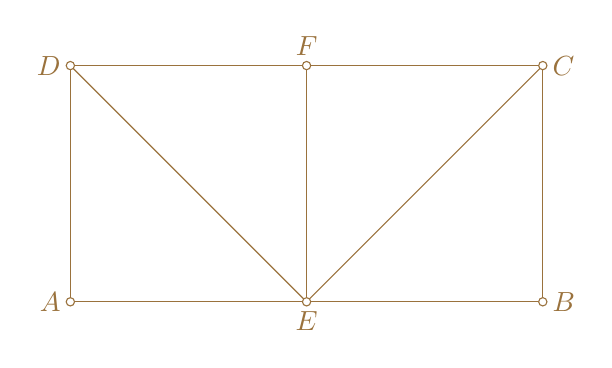
\begin{tikzpicture}[scale=0.75,lichsutoanhoc]
			\draw (0,0) rectangle (8,4);
			\draw (0,4) -- (4,0) -- (8,4);
			\draw (4,0) -- (4,4);
			\draw [fill = white] (0,0) circle (2.0pt) node[left] {$A$};
			\draw [fill = white] (0,4) circle (2.0pt) node[left] {$D$};
			\draw [fill = white] (4,0) circle (2.0pt) node[below] {$E$};
			\draw [fill = white] (4,4) circle (2.0pt) node[above] {$F$};
			\draw [fill = white] (8,4) circle (2.0pt) node[right] {$C$};
			\draw [fill = white] (8,0) circle (2.0pt) node[right] {$B$};
		\end{tikzpicture}
		\vspace*{-10pt}
	\end{figure}
	Gọi $E$, $F$ lần lượt là trung điểm $AB$ và $CD$. Khi ấy $\Delta ADE = \Delta BCE$ (c.g.c), góc bằng nhau ở đỉnh $A$ và $B$. Từ đây có: $ \angle AED = \angle BEC, \angle ADE = \angle BCE, DE = CE$. Theo Saccheri $1$, $ \angle ADC = \angle BCD$, kết hợp lại ta được:
	\begin{align*}
		\angle EDF &= \angle EDC = \angle ADC - \angle ADE \\
		&= \angle BCD - \angle BCE \\
		&= \angle ECD = \angle ECF.
	\end{align*}
	Do đó $ \Delta DFE = \Delta CFE$ (c.g.c), suy ra $ \angle DFE = \angle CFE$. Hai góc này bù nhau nên chúng là góc vuông.
	Cũng có $ \angle DEF = \angle CEF$, cộng với $ \angle DEA = \angle CEB$ có $ \angle FEA = \angle FEB$, $ \angle FEA$ bằng với góc bù với nó nên là góc vuông nốt.
	\vskip 0.1cm
	Có thể thấy Saccheri đã hé mở cánh cửa tới một loại hình học nơi mà tiên đề song song bị bác bỏ, và dù ông đã hấp tấp đóng nó lại vì niềm tin vốn có, ý tưởng sử dụng phản chứng ông đưa ra là một bước tiến lớn. Trong số tiếp theo, chúng ta sẽ tìm hiểu quá trình khám phá của những người mở đường vào thế giới sau khe cửa hẹp đó. 
	\vskip 0.1cm
	\textbf{\color{lichsutoanhoc}Tài liệu tham khảo}
	\vskip 0.1cm
	-- Wikipedia tiếng Anh.
	\vskip 0.1cm
	-- Euclidean and Non--Euclidean Geometries -- Development and History (Marvin Jay Greenberg).
	\vskip 0.1cm
	-- Men of Mathematics The Lives and Achievements of the Great Mathematicians from Zeno to Poincaré (Eric Temple Bell).
	\vskip 0.1cm
	-- The History of Mathematics An Introduction (David M. Burton).
	\vskip 0.1cm
	-- https: //www.youtube.com/playlist?list=PL\\jLK2cYtt-VBSBtvfhxx-DW3Zw3nOQHVZ
	\vskip 0.1cm
	-- https: //rosetta.vn/lequanganh/wp-conten\\t/
	uploads/sites/7/2018/07/Riemann.pdf
	\vskip 0.1cm
	-- https: //www.cut-the-knot.org/triangle/py\\
	thpar/Drama.shtml
\end{multicols}


	\newpage

	\setcounter{figure}{0}
	 \thispagestyle{gocconone}
\pagestyle{gocco}
\everymath{\color{gocco}}
\graphicspath{{../gocco/pic/}}
\blfootnote{$^1${\color[named]{gocco}Đại kiện tướng quốc tế.}}
\begingroup
\AddToShipoutPicture*{\put(0,616){\includegraphics[width=19.3cm]{../bannergocco}}}
\AddToShipoutPicture*{\put(96,525){\includegraphics[scale=1]{../tieude.pdf}}} 
\centering
\endgroup

\vspace*{185pt}

\begin{multicols}{2}
	Lý thuyết cờ tàn cơ bản đều cho rằng xe và tượng chống xe không có tốt đều được coi là hòa cờ cơ bản. Tuy nhiên thực tế thi đấu cho thấy khả năng hòa cờ cho bên yếu không nhiều. Bên yếu cần phải chơi rất chính xác nếu muốn gỡ hòa.
	Trong bài học hôm nay, chúng tôi xin trình bày một số tình huống cơ bản 
	\vskip 0.1cm
	\textbf{\color{gocco}A.	Philidor}
	\begin{center}
		\newgame
		\fenboard{3k4/4r3/3K4/3B4/8/8/8/5R2 b Q - 0 1}
		\scalebox{0.85}\showboard
		\vskip 0.1cm
		\textit{\small\color{gocco}Hình $1$. Trắng đi trước thắng, $1749$.}
	\end{center}
	\textbf{\color{gocco}$\pmb{1}$.Xf$\pmb{8}$+ Xe$\pmb{8}$ $\pmb{2}$.Xf$\pmb{7}$ Xe$\pmb{2}$ $\pmb{3}$.Xh$\pmb{7}$} (Hình $2$) [Một nước đi chờ đợi]
	\vskip 0.1cm
	\textbf{\color{gocco}$\pmb{3}$...Xe$\pmb{1}$ $\pmb{4}$.Xb$\pmb{7}$! Xc$\pmb{1}$} [$4$...Vc$8$ $5$.Xa$7$ Xb$1$ $6$.Xh$7$! 
	\vskip 0.1cm
	$6$...Vb$8$ $7$.Xh$8$+ Va$7$ $8$.Xa$8$+ Vb$6$ $9$.Xb$8$+ Va$5$ $10$.Xxb$1$]
	\vskip 0.1cm
	\textbf{\color{gocco}$\pmb{5}$.Tb$\pmb{3}$!!} 
	\begin{center}
		\newgame
		\fenboard{2k5/7R/3K4/3B4/8/8/8/1r6 b Q - 0 1}
		\scalebox{0.85}\showboard
		\vskip 0.1cm
		\textit{\small\color{gocco}Hình $2$.}
	\end{center}
	\begin{center}
		\newgame
		\fenboard{3k4/1R6/3K4/8/8/1B6/8/2r5 b Q - 0 1}
		\scalebox{0.85}\showboard
		\vskip 0.1cm
		\textit{\small\color{gocco}Hình $3$.}
	\end{center}
	\textit{Kỹ thuật giành chiến thắng cơ bản của bên có tương là tìm cách ép vua đối phương xuống hàng ngang số $8,1$ hoặc cột a,h. Sau đó phối hợp giữa xe và tượng thực hiện vừa che chắn cho vua khỏi các nước chiếu của xe đối bằng tượng trong khi đó dùng xe đe dọa chiếu hết.}
	\vskip 0.1cm
	\textbf{\color{gocco}$\pmb{5}$...Xc$\pmb{3}$ $\pmb{6}$.Te$\pmb{6}$! Xd$\pmb{3}$+ $\pmb{7}$.Xd$\pmb{5}$} [Tượng trắng che chắn cho vua]
	\vskip 0.1cm
	$7$...Xc$3$ $8$.Xd$7$+ Vc$8$ $9$.Xh$7$ Vb$8$ $10$.Xb$7$+ Vc$8$ $11$.Xb$4$ Vd$8$ $12$.Tc$4$!! (Hình $4$). Trắng dùng Tượng ngăn cản xe đối phương phòng thủ ở ô c$8$.
	\begin{center}
		\newgame
		\fenboard{3k4/8/3K4/8/1RB5/2r5/8/8 b Q - 0 1}
		\scalebox{0.85}\showboard
		\vskip 0.1cm
		\textit{\small\color{gocco}Hình $4$.}
	\end{center}
	Trắng đe dọa chiếu hết ở nước tiếp theo
	\vskip 0.1cm
	\textbf{\color{gocco}$\pmb{12}$...Vc$\pmb{8}$} [$12$...Ve$8$ $13$.Xb$8\#$]
	\vskip 0.1cm
	\textbf{\color{gocco}$\pmb{13}$.Te$\pmb{6}$+ Vd$\pmb{8}$ $\pmb{14}$.Xb$\pmb{8}$+}
	\vskip 0.1cm
	\textbf{\color{gocco}Lolli}
	\begin{center}
		\newgame
		\fenboard{2k5/3r4/2K5/2B5/8/8/8/4R3 b Q - 0 1}
		\scalebox{0.85}\showboard
		\vskip 0.1cm
		\textit{\small\color{gocco}Hình $5$. Trắng đi trước thắng, $1763$.}
	\end{center}
	Trong rất nhiều trường hợp mặc dù xe đen cũng phòng thủ từ phía sau hoặc bên sườn, tuy nhiên bên mạnh cũng vẫn thắng.
	\vskip 0.1cm
	\textbf{\color{gocco}$\pmb{1}$.Xe$\pmb{8}$+ Xd$\pmb{8}$ $\pmb{2}$.Xe$\pmb{7}$ Xd$\pmb{2}$} [Nếu $2$...Xh$8$ $3$.Td$6$ Vd$8$ $4$.Xa$7$ Ve$8$ $5$.Xa$8+$; Nếu $2$...Xg$8$ $3$.Td$6$ Vd$8$ $4$.Xe$6$! (Hình $6$)
	\begin{center}
		\newgame
		\fenboard{3k2r1/8/2KBR3/8/8/8/8/8 b Q - 0 1}
		\scalebox{0.85}\showboard
		\vskip 0.1cm
		\textit{\small\color{gocco}Hình $6$.}
	\end{center}
	$4$...Vc$8$ ($4$...Xh$8$ $5$.Te$5$ Xf$8$ $6$.Tg$7$! Trắng giam xe đen ở hàng ngang số $8$
	\begin{center}
		\newgame
		\fenboard{3k1r2/6B1/2K1R3/8/8/8/8/8 b Q - 0 1}
		\scalebox{0.85}\showboard
		\vskip 0.1cm
		\textit{\small\color{gocco}Hình $7$.}
	\end{center}
	$6$...Xg$8$ $7$.Tf$6$+ Vc$8$ $8$.Xe$4$ Xf$8$ $9$.Tg$7$ Xg$8$ $10$.Xa$4$ Vb$8$ (\textit{$10$...Vd$8$ $11$.Xa$8$+}) $11$.Te$5$+ Vc$8$ $12$.Xa$8\#$) $5$.Xe$5$ Vd$8$ $6$.Tc$7$+ Vc$8$ $7$.Xa$5$ Xg$6$+ $8$.Td$6$+–]
	\vskip 0.1cm
	\textbf{\color{gocco}$\pmb{3}$.Xf$\pmb{7}$! Xd$\pmb{1}$} [$3$...Xd$8$ $4$.Te$7$ Xg$8$ $5$.Xf$5$ Vb$8$ $6$.Td$6$+ Vc$8$ $7$.Xa$5$]
	\vskip 0.1cm
	\textbf{\color{gocco}$\pmb{4}$.Xa$\pmb{7}$ Xb$\pmb{1}$} [$4$...Vb$8$ $5$.Xa$4$ Xc$1$ $6$.Xe$4$!]
	\begin{center}
		\newgame
		\fenboard{2k5/R7/2K5/8/8/B7/8/1r6 b Q - 0 1}
		\scalebox{0.85}\showboard
		\vskip 0.1cm
		\textit{\small\color{gocco}Hình $8$.}
	\end{center}
	$5$.Ta$3$!! 
	\vskip 0.1cm
	Nước cờ chìa khóa. Đen bị ``xung xoang" vì không có nước đi cho xe. 
	\vskip 0.1cm
	\textbf{\color{gocco}$\pmb{5}$...Xb$\pmb{3}$} [Phương án khác cũng không tốt hơn cho đen $5$...Vb$8$ $6$.Xe$7$ Va$8$ $7$.Xe$4$!! Xb$7$! $8$.Xe$5$ 
	\vskip 0.1cm
	Đen bị ``xung xoang" $8$...Xf$7$ ($8$...Xb$1$ $9$.Xa$5$+ Vb$8$ $10$.Td$6$+ Vc$8$ $11$.Xa$8$+) $9$.Xe$8$+ Va$7$ $10$.Tc$5$+ Va$6$ $11$.Xa$8$+ Trắng thắng]
	\begin{center}
		\newgame
		\fenboard{k7/1r6/2K5/4R3/8/B7/8/8 b Q - 0 1}
		\scalebox{0.85}\showboard
		\vskip 0.1cm
		\textit{\small\color{gocco}Hình $9$.}
	\end{center}
	\textbf{\color{gocco}$\pmb{6}$.Td$\pmb{6}$! Xc$\pmb{3}$+ $\pmb{7}$.Tc$\pmb{5}$}  
	\vskip 0.1cm
	Tượng trắng phối hợp với vua và xe. Tượng vừa thực hiện việc che chắn cho vua và tấn công vua đối phương.
	\begin{center}
		\newgame
		\fenboard{2k5/R7/2K5/2B5/8/2r5/8/8 b Q - 0 1}
		\scalebox{0.85}\showboard
		\vskip 0.1cm
		\textit{\small\color{gocco}Hình $10$.}
	\end{center}
	\textbf{\color{gocco}$\pmb{7}$...Xb$\pmb{3}$ $\pmb{8}$.Xc$\pmb{7}$+ Vb$\pmb{8}$} [$8$...Vd$8$ $9$.Xf$7$]
	\vskip 0.1cm
	\textbf{\color{gocco}$\pmb{9}$.Xe$\pmb{7}$ Va$\pmb{8}$ $\pmb{10}$.Xe$\pmb{4}$!} [$10$.Xe$8$+ Xb$8$ $11$.Xe$1$]
	\vskip 0.1cm
	\textbf{\color{gocco}$1\pmb{0}$...Xb$\pmb{7}$ $\pmb{11}$.Xa$\pmb{4}$+ Vb$\pmb{8}$ $\pmb{12}$.Td$\pmb{6}$+ Vc$\pmb{8}$ $\pmb{13}$.Xa$\pmb{8}$+} Trắng thắng
\end{multicols}
\vspace*{-10pt}
{\rule{1\linewidth}{0.1pt}}
\vskip 0.2cm
\centerline{\LARGE\textbf{\color{gocco}LỜI GIẢI, ĐÁP ÁN}}
\begin{multicols}{2}
	 Về một người đã được đánh dấu, ta đã biết chắc anh ta không phải là $Z$, vì hoặc anh ta không biết ai đó, hoặc ai đó biết anh ta. Sau khi đưa ra tất cả các câu hỏi (chúng không quá $(n-2)$ câu), số những người chưa được đánh dấu không ít hơn $2$. 
	\vskip 0.1cm
	Giả sử $X$ là một trong số những người chưa được đánh dấu. Sau khi đưa ra tất cả các câu hỏi, ta đã có một số thông tin về ai biết ai. Ta sẽ thay đổi toàn bộ hệ thống quen biết, sao cho các thông tin đã có  thì vẫn giữ nguyên, tuy nhiên $X$ sẽ biến thành $Z$. Khi đó, ta sẽ làm cho $X$ biết tất cả mọi người, còn trong tất cả những trường hợp còn lại (trừ những trường hợp quen biết đã được xác định trước đó) ta sẽ đều coi là không ai biết ai.
	\vskip 0.1cm
	Như vậy, đối với một người chưa được đánh dấu bất kỳ ($X$ được chọn ra trong số họ một cách tuỳ ý), luôn có thể thay đổi hệ thống quen biết để sao cho chính anh ta là $Z$. Và điều này có nghĩa là với ít hơn $(n-1)$ câu hỏi không đủ để làm rõ được ai là $Z$.
\end{multicols}
	\newpage

%	\thispagestyle{empty}
%	\begingroup 
%	\AddToShipoutPicture*{\put(0,0){\includegraphics[width=19.3cm]{dovui.pdf}}}
%	\centering
%	\vspace*{0cm}
%	\endgroup
%	\newpage	
%	\pagestyle{empty}
\end{document} 
